\documentclass[a4paper,11pt]{article}
\usepackage[italian]{babel} 
\usepackage[T1]{fontenc} 
\usepackage[utf8]{inputenc} \usepackage[margin=1.in,left=1.in,includefoot]{geometry}
\usepackage{amsmath,amssymb,amsthm}
\usepackage{graphicx,color,listings}
\usepackage{mathtools}
\usepackage[usenames,dvipsnames]{xcolor}
\usepackage[colorlinks=true, linkcolor=black, citecolor=black, urlcolor=black, filecolor=black]{hyperref}
\usepackage{physics}
\usepackage{dsfont}
\usepackage{enumitem}
\usepackage{setspace}
\usepackage{midpage}
\usepackage{movie15}
%\usepackage{SIunits}
\usepackage{subfig}
\usepackage{wrapfig}
\frenchspacing 


\renewcommand{\figurename}{Fig.}
\renewcommand\qedsymbol{Q.E.D.}
\renewcommand{\grad}{\Vec{\nabla}}
\renewcommand{\div}{\Vec{\nabla}\cdot}
\renewcommand{\epsilon}{\varepsilon}

\newcommand{\hu}{\hat{u}}
\newcommand{\p}{\partial}
\newcommand{\V}{\scriptscriptstyle{V}}
\newcommand{\R}{\mathbb{R}}
\newcommand{\N}{\mathbb{N}}
\newcommand{\Z}{\mathbb{Z}}
\newcommand{\Q}{\mathbb{Q}}
\newcommand{\C}{\mathbb{C}}
\newcommand{\serie}{\displaystyle\sum_{n=1}^\infty}
\newcommand{\serio}{\displaystyle\sum_{n=0}^\infty}
\newcommand{\Sum}{\displaystyle\sum}
\newcommand{\limite}{\displaystyle\lim_{n\to \infty}}
\newcommand{\limi}{\displaystyle\lim}
\newcommand{\limixy}{\displaystyle\lim_{\substack{ x\to 0\\y\to 0}}}
\newcommand{\mc}{\mathcal}
\newcommand{\inte}{\displaystyle\int}
\newcommand{\Ap}{\mathcal{A^*}}
\newcommand{\nepero}{\left(1+\frac{1}{n}\right)^n}
\newcommand{\nn}{\forall n\in\mathbb{N}}
\newcommand{\rot}{\Vec{\nabla}\times}
\newcommand{\f}{\varphi}


%\setlength\parindent{0pt}

\begin{document}


\begin{titlepage}
  \begin{midpage}
       \begin{center}
      
      \vspace{2 cm}    
      \centerline{\hbox to 3.5 cm {\hrulefill}}
      \medskip
      \medskip
      \textsc{ \Huge Astrofisica}
      \centerline{\hbox to 3.5 cm {\hrulefill}}
      \vspace{3 cm}
     
      
      \vspace{8.9 cm}
      \textsc{A.A. 2022/2023}
      
        \end{center}
 \end{midpage}
\end{titlepage}

\newpage
\pagenumbering{Roman}
\tableofcontents
\newpage
\pagenumbering{arabic}


\section{Lezione del 3/10}
\subsection{Astrofisica in Italia}
Questo è un corso che dovrebbe dare una visione generale dell'astrofisica, non è un corso specialistico, cercherò di darvi una panoramica dell'astrofisica. Non guardiamo al telescopio, si faceva 200 anni fa, al telescopio si acquisiscono dati, ormai non c'è neanche un posto per mettere l'occhio al telescopio.\\
Secondo wikipedia l'astrofisica è praticamente tutto
\begin{center}
   L'astrofisica è la branca della fisica e dell'astronomia che studia le proprietà fisiche, ossia tutti i vari fenomeni, della materia celeste. 
\end{center}
\begin{itemize}
    \item Come fare astrofisica.
    \item Dove fare astrofisica.
    \item A che livello la faccio.
\end{itemize}
Cosa è l'astrofisica in Italia? Dove si svolge?\\
Essa si svolge presso l'istituto nazionali di astrofisica INAF che ha 19 istituti dislocati nelle più grandi città italiane, a Catania abbiamo l'osservatorio astrofisico di Catania. Nella valle di Noto abbiamo un istituto di radioastronomia dove c'è un radiotelescopio. 

L'astrofisica può essere svolta sotto molti aspetti, per esempio è svolta all'interno dell'Agenzia Spaziale Italiana ASI dove si lanciano satelliti che hanno obiettivi: sorveglianza ambientale geologia e principalmente osservazioni astrofisiche. L'Italia fa parte dell'European Southern Observatory ESO, consorzio europeo con sede in Germania ha i telescopi in Cile, il Sud del mondo vede il centro della galassia, si vedono molte più stelle che all'emisfero boreale.\\
L'Italia è il quinto paese al mondo per pubblicazioni, inoltre nel 2002 il professore Giacconi dell'università di Milano ha preso il nobel per l'astrofisica. L'astrofisica è una scienza osservativa, molti paesi europei non hanno attrezzature scientifiche di tipo osservativo perché è necessario un clima adatto, poca piovosità. In Italia abbiamo un clima favorevole, all'inizio del '900 i nord europei vennero a chiedere gli strumenti in Italia. I climi migliori sono nelle zone desertiche o nelle isole come le Hawaii. In Italia abbiamo molti osservatori dove si possono imparare le basi.\\
L'INAF ha molte strutture in tutte il mondo.
\begin{figure}[ht]
    \centering
    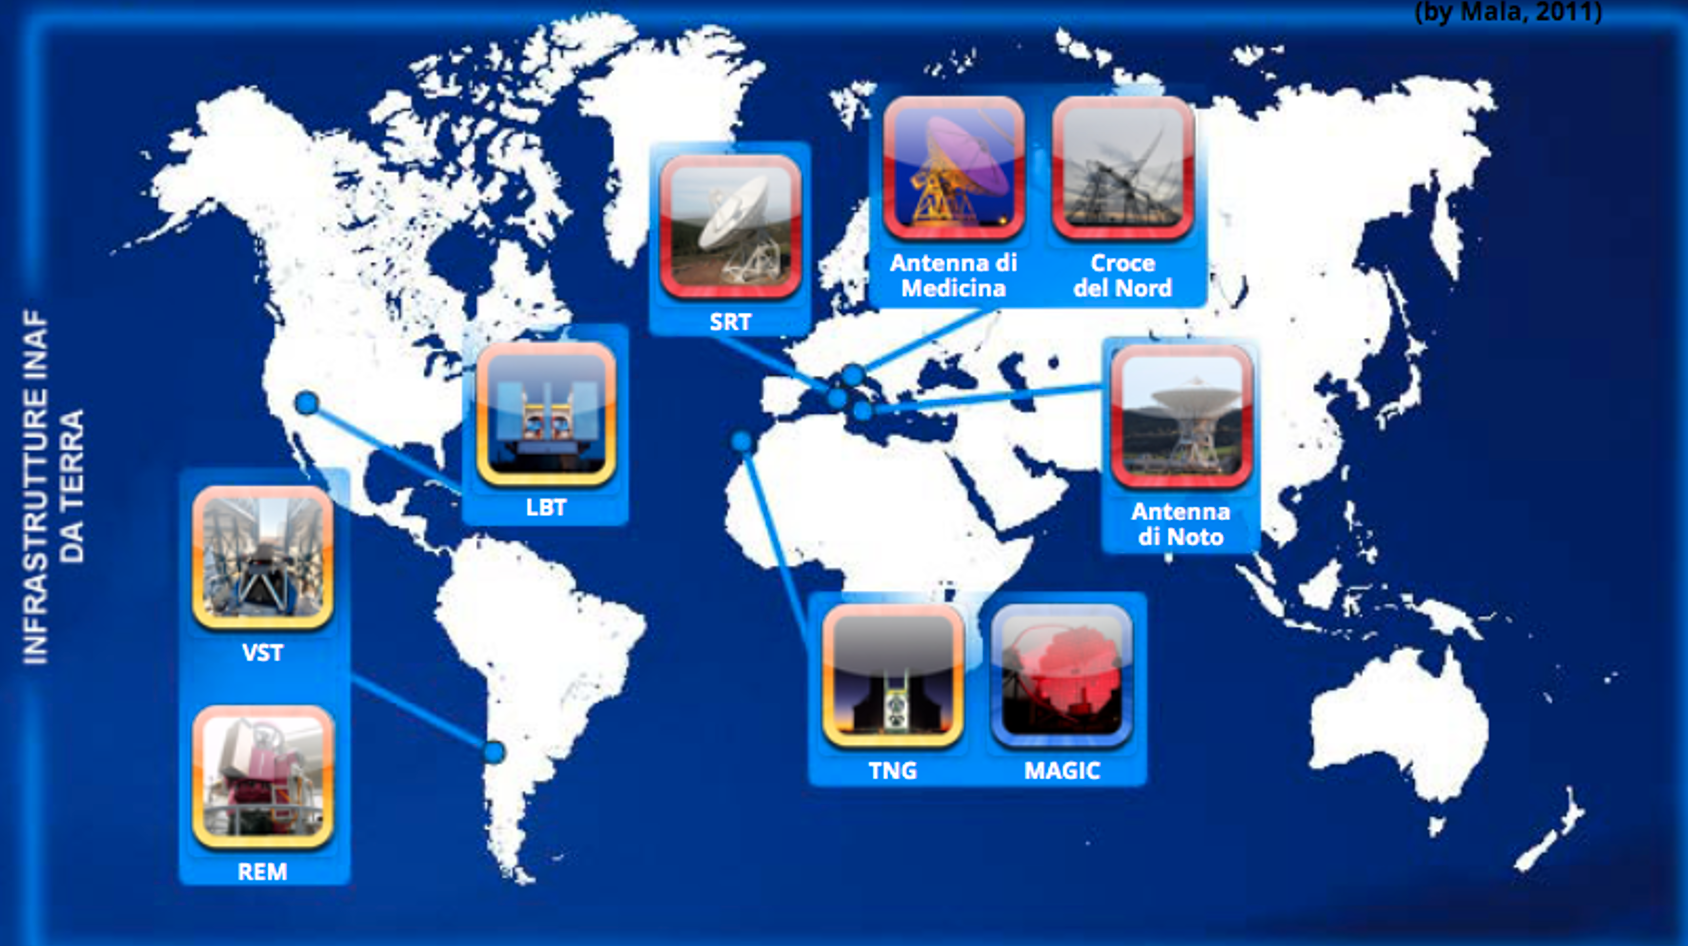
\includegraphics[width=12 cm]{Strutture inaf.png}
\end{figure}
\begin{itemize}
    \item Telescopio Nazionale Galileo Galilei (TNG) nell'isola di La Palma alle Canarie con un diametro di 3.5 metri. 
    \item Large Binocular Telescope due telescopi da 8 metri in Arizona
    \item Osservatorio del Paranal 4 da 8 metri e 8 da 3 metri mobili che si muovo su dei binari.
    \item Telescopi al polo sud.
\end{itemize}
Non è solo astrofisica ottica, radiotelescopi italiani.
\begin{itemize}
    \item Osservatorio di Noto da 32 metri.
    \item Sardinia Radio Telescope (SRT) da 64 metri. Specializzato nell'osservazione delle pulsar.
\end{itemize}
Italia invidiata perché i nostri istituti comunicano e vengono coordinati dall'ente centrale. Si possono organizzare facilmente osservazioni multiple in contemporanea.\\
L'Atacama Large Millimeter/submillimeter Array è l'osservatorio radio migliore al mondo.\\
L'attività spaziale è fondamentale perché l'atmosfera terrestre è un forte filtro per la radiazione elettromagnetica, passa poco.
\begin{figure}[ht]
    \centering
    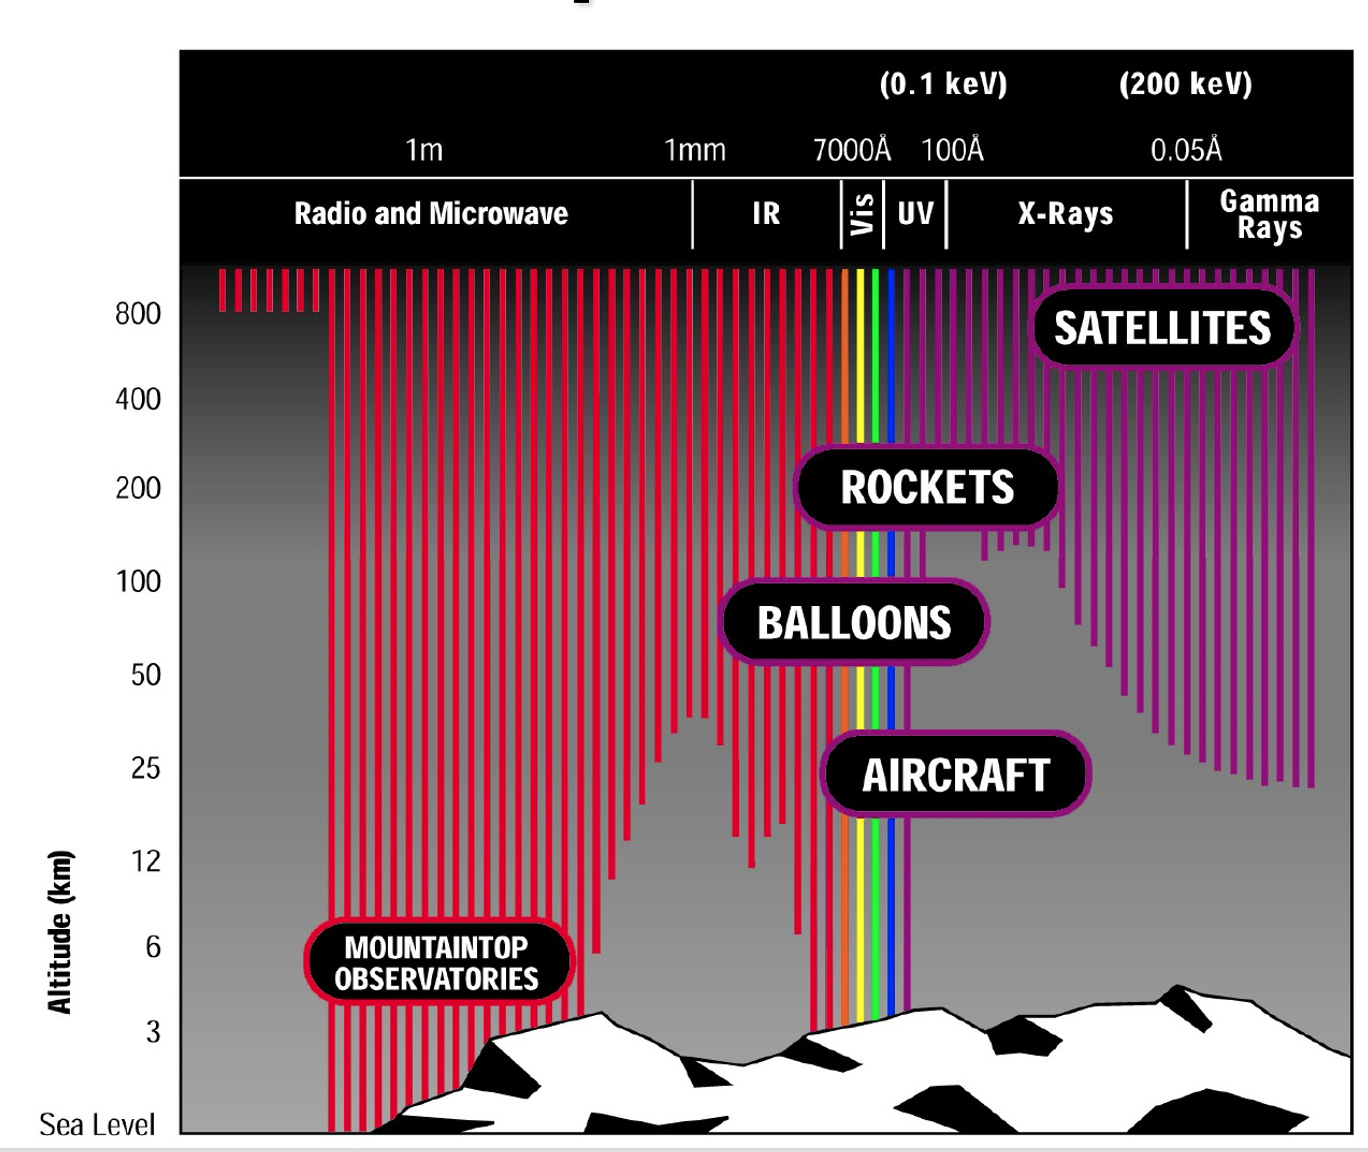
\includegraphics[width=8 cm]{Radiazione-atmosfera.png}
\end{figure}
L'Italia partecipa a molte missioni spaziali. L'Italia ha molta esperienza nelle missioni spaziali, negli anni 60 eravamo capaci di lanciare satelliti, oggi facciamo strumenti per i satelliti, veniamo richiesti per la costruzione della strumentazione.

\subsection{Fisica vs astrofisica}
 Un fisico va in laboratorio cambia le condizioni a contorno del proprio campione, l'astrofisico non ha questa possibilità, deve dedurre le proprietà del proprio oggetto solo osservando. Questa differenza prevede delle ipotesi, cioè le leggi della fisica che valgono sulla Terra valgono ovunque. Non sappiamo se è vero. Per esempio abbiamo applicato la gravità di Newton per secoli, quando l'abbiamo applicata all'orbita Mercurio non era valida perché ha deformazioni relativistiche. Uno deve fare delle ipotesi che siano ragionevoli. Si suppone che leggi della fisica valgano ovunque.\\
 Un altro problema è che osservo oggetti che non cambiano nella generalità. Uno deve decidere come funzionano le cose guardando una foto, dovremmo interpretare fenomeni che avvengono su tempi scala troppo lunghi rispetto alla vita umana, noi conosciamo la fisionomia umana possiamo facilmente riconoscere se una persona è più anziana o meno di un'altra. Per gli oggetti astronomici non è così. Inoltre l'informazione si trasferisci con una velocità finita quindi un oggetto lontano è più giovane perché l'informazione necessità di più tempo. Dalle osservazioni dobbiamo trovare delle regolarità, che può anche essere temporale, la vera difficoltà dell'astrofisica è mettere tutte queste informazioni e fare un quadro in evoluzione con oggetti diversi. Questo si fa studiando alcuni oggetti molto in dettaglio.

\subsection{Scopi dell'astrofisica}
\begin{itemize}
    \item Come si evolvono stelle e pianeti?
    \item Esiste la vita fuori dal sistema solare?
    \item Di cosa è fatto l'universo?
    \item Cosa è successo all'inizio dell'universo?
    \item Come è fatto un buco nero?
    \item Cosa accade allo spazio-tempo quando oggetti cosmici collidono?
\end{itemize}
In questo corso tratteremo i seguenti argomenti
\begin{itemize}
    \item Principi di diagnostica dei plasmi.
    \item Tecniche astrofisiche di raccolta dati.
    \item Stelle e mezzo interstellare.
    \item Il sole e il sistema solare.
    \item La nostra galassia.
    \item Cosmologia.
\end{itemize}

\subsection{Tempo astronomico}
Agli inizi vedere un oggetto spostarsi in cielo ha dato vita all'astronomia. Questo ha portato alla definizione di \textbf{tempo} e alla nascita degli attuali sistemi di riferimento. Il tempo è stato definito tramite il sorgere e il tramontare del sole per scandire le giornate. Questo ha portato alla nascita delle meridiane, uno dei primi strumenti per misurare oggettivamente il tempo.\\
La durata del \textbf{giorno solare} è stata definita come il tempo che il sole impiega a rioccupare la stessa posizione relativamente alla Terra e durava 24 ore.\\
Se osserviamo il moto di una stella attorno alla polare, ci accorgeremmo che non ci impiega 24 ore ma 23 ore 56 minuti e  4.1 secondi; questa è la durata del \textbf{giorno siderale}.
Questo ha portato alla comprensione che era la terra a girare intorno al Sole, la differenza fra giorno solare e siderale è dovuta all'orbita della Terra.
\begin{figure}[ht]
    \centering
    %\includegraphics[width=8 cm]{Giorno solare e siderale.png}
\end{figure}
Analogamente è stato definito l'\textbf{anno sidereo}, esso è il tempo che deve trascorrere affinché il sole rioccupi la stessa posizione rispetto alle stelle. Il sole nel suo moto apparente passa attraverso alcune costellazioni chiamate costellazioni zodiacali. L'anno sidereo dura 365 giorni 6 ore 9 minuti 9.54 secondi; per comodità si usa solo la parte intera e ogni quattro anni si aggiunge un giorno (anno bisestile).\\
Questo metodo di suddivisione del tempo è scomodo per gli astronomi, perché è un metodo frazionario. Si è deciso di utilizzare le frazioni del giorno, 12 ore sono 0.5 giorni. Serve uno zero dell'asse dei tempi, esso è stato posto alla \textbf{data Juliana}. La data Juliana è il contare il tempo in giorni a partire dalle ore 12:00 dell'1 gennaio del 4713 a.C. di Greenwich, questo agevola molto i conti. La data juliana cambia a mezzogiorno perché così non cambia la data durante la stessa notte di osservazione. Questo metodo da una continuità al tempo. È stato proposto il 4713 il Sole, a causa della precessione, si trovava nell'esatto punto quando lui aveva fatto la proposta; in realtà venne accolta perché non c'è nessuna traccia astronomica prima di tale data. \\
Guardando il cielo si è resi conto che l'altezza del Sole in estate è molto più alta che in inverno nell'emisfero boreale. Da questo si è dedotto che l'asse di rotazione della terra è inclinato rispetto all'orbita terrestre, con il variare dell'altezza del sole cambiano le stagioni. A marzo ha un'altezza media, a giugno ha l'altezza massima e così via.
L'inclinazione dell'asse terrestre è di $23.45^\circ$. Abbiamo definito l'anno l'abbiamo suddiviso in stagioni e in giorni.

\subsection{Coordinate astronomiche}
Per identificare le stelle in cielo sono state divise in costellazioni, le costellazioni sono una appartenenza ad un gruppo di stelle legato alla visualizzazione di figure (Cefeo, Orsa Maggiore, Orione ecc...), questo vale per le stelle molto luminose e richiede una conoscenza molto generale. E' auspicabile identificare le stelle in maniera più esatta. I cinesi hanno diviso il cielo in quadranti regolari, quindi di più facile utilizzo ma il problema che dobbiamo risolvere è identificare esattamente una stella in un quadrante di cielo molto piccolo per identificare singolarmente ogni stella. Per fare ciò serve un sistema di riferimento. Il sistema di riferimento naturale è quello in cui il piano in cui ci troviamo diventa il nostro orizzonte, vi è un punto privilegiato chiamato \textbf{zenith}. Gli oggetti appaiono sulla sfera celeste in cui non hanno distanze possiamo immaginare di identificare la posizione di un oggetto di semplici coordinate sferiche, bastano due coordinate. Il cerchio massimo passante per lo zenith e la Polare è detto \textbf{meridiano principale}, se guardiamo in direzione opposta alla polare sul cerchio massimo guardiamo il Sud, cioè dove culmina il Sole. Abbiamo identificato una direzione privilegiata.\\
Definiamo le \textbf{coordinate altazimutali}:
\begin{itemize}
    \item \textbf{Altezza:} distanza angolare dell'oggetto dall'orizzonte.
    \item \textbf{Azimut:} distanza angolare del meridiano passante per la stella e il meridiano principale.
\end{itemize}
\begin{figure}[ht]
    \centering
    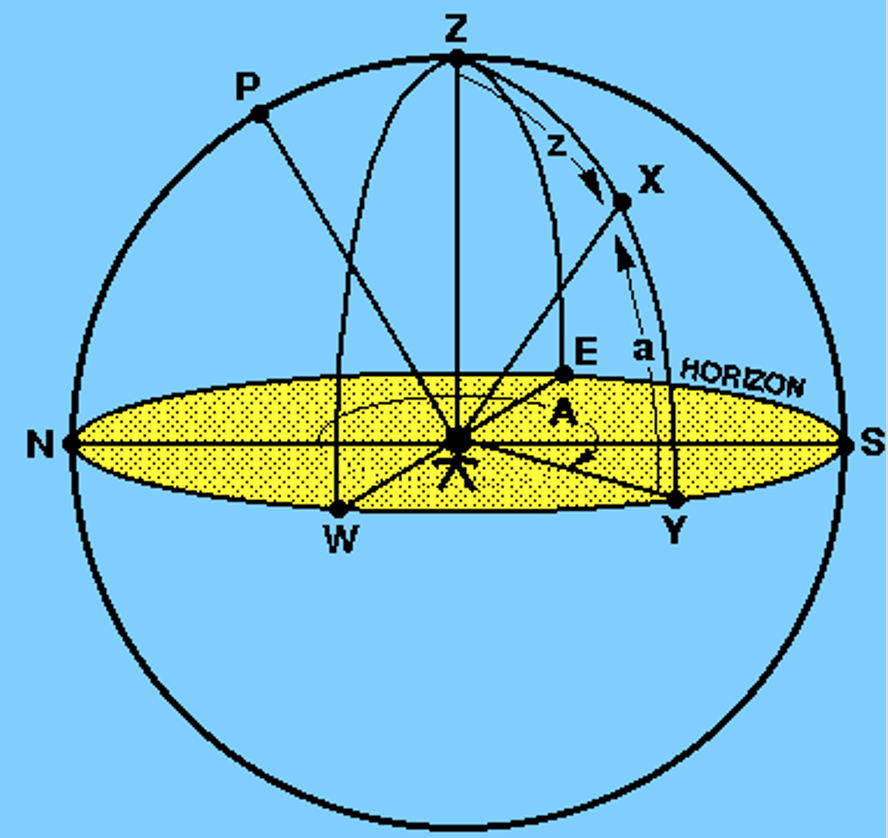
\includegraphics[width=5 cm]{Coordinate altazimutali.png}
\end{figure}
Possiamo definire analogamente la \textbf{distanza zenitale} come la distanza angolare dell'oggetto dallo zenith.\\
Il problema di questo sistema di riferimento è che cambia in base alla posizione dell'osservatore. Per esempio al polo Nord la polare ha una altezza di $90^\circ$, se sto all'equatore la polare ha un'altezza di $0^\circ$. 
\begin{figure}[ht]
    \centering
    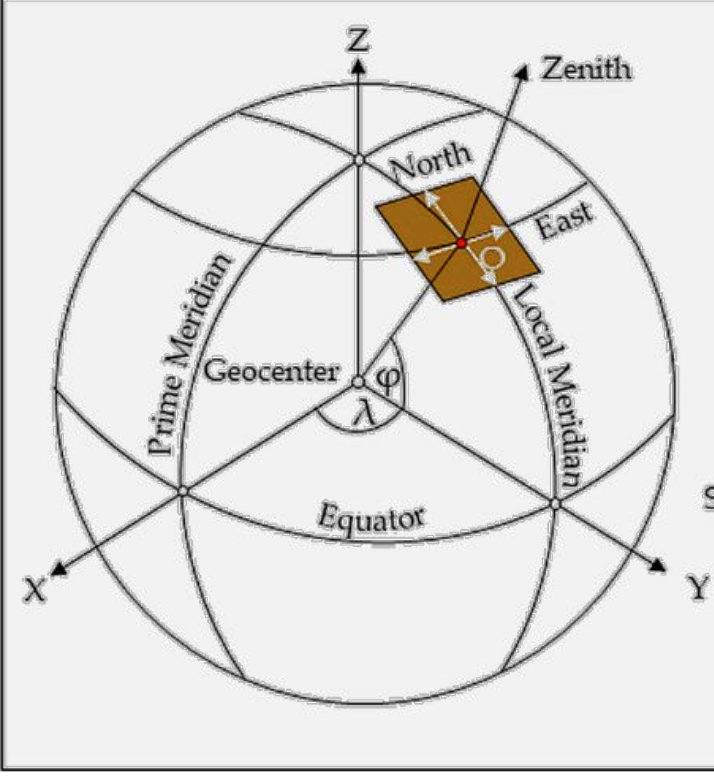
\includegraphics[width=5 cm]{Piano dell'orizzonte sulla terra.png}
\end{figure}
Inoltre durante lo scorrere del tempo azimut e altezza cambiano continuamente, gli oggetti si muovono di 15 gradi all'ora. È un sistema necessario quando costruisco qualcosa ma è inutile nell'utilizzo.\\
Sarebbe più interessante avere un sistema di riferimento comune, poniamo  l'orizzonte coincidente con l'equatore rotazionale terrestre, tutti abbiamo lo stesso equatore. Se definiamo un meridiano comune a tutti l'altezza sull'orizzonte di un oggetto sull'orizzonte è comune a tutti, chiamiamo \textbf{declinazione} l'altezza sull'orizzonte dell'oggetto, la declinazione è una proprietà dell'oggetto non più dell'osservatore. Siccome le stelle sono ferme (è la terra che gira), con una opportuna convenzione, il nuovo azimut è un \textbf{angolo orario} $H$ perché cambierà con il ruotare della Terra quindi dall'ora del luogo. Per noi il sistema di riferimento è l'orario di Greenwich. Possiamo dire che se una stella si trova sul meridiano di Greenwich ha angolo orario 0. 
\begin{figure}[ht]
    \centering
    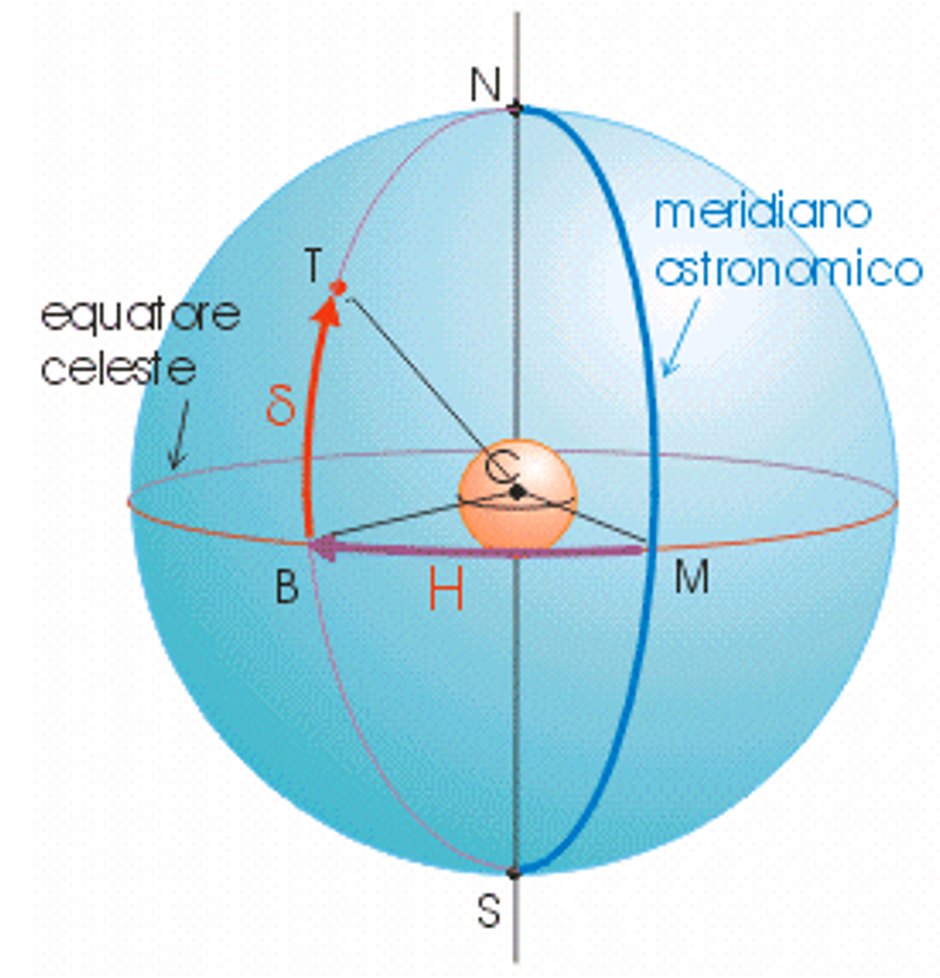
\includegraphics[width=5 cm]{Coordinate orarie.png}
\end{figure}
Se so dove sono localizzato come time zone possiamo conoscere l'angolo orario e puntare lo stesso oggetto, basta sommare il fuso orario all'angolo orario e l'angolo orario diventerebbe una coordinata insieme alla declinazione indipendente dal posto in cui si trova l'osservatore. Ha ancora uno svantaggio: la Terra ruota intorno al Sole. Un sistema migliore sarebbe un sistema esterno solidale con la Terra, dove l'angolo orario non sia legato a Greenwich ma dovremmo trovare un riferimento legato alla posizione occupata dal Sole in un determinato periodo dell'anno. Il piano equatoriale interseca il piano orbitale della Terra in due punti chiamati \textbf{nodi}, il Sole passa dal basso in alto all'equatore in primavera chiamiamo questo punto \textbf{punto $\gamma$}, in autunno  accade l'opposto, il Sole passa da declinazioni positive a declinazioni negative questo punto verrà chiamato \textbf{punto $\Omega$}. Al posto di prendere il meridiano di Greenwich che gira insieme alla Terra, ma abbiamo definito un punto fisso nel cielo, il punto $\gamma$. Chiamiamo la coordinata della stella \textbf{ascensione retta} $\alpha$, l'angolo fra la posizione della stella e il punto gamma nel piano equatoriale. Essa diventa una misura oggettiva della posizione, non dipende dal luogo e dall'orario. 
\begin{figure}[ht]
    \centering
    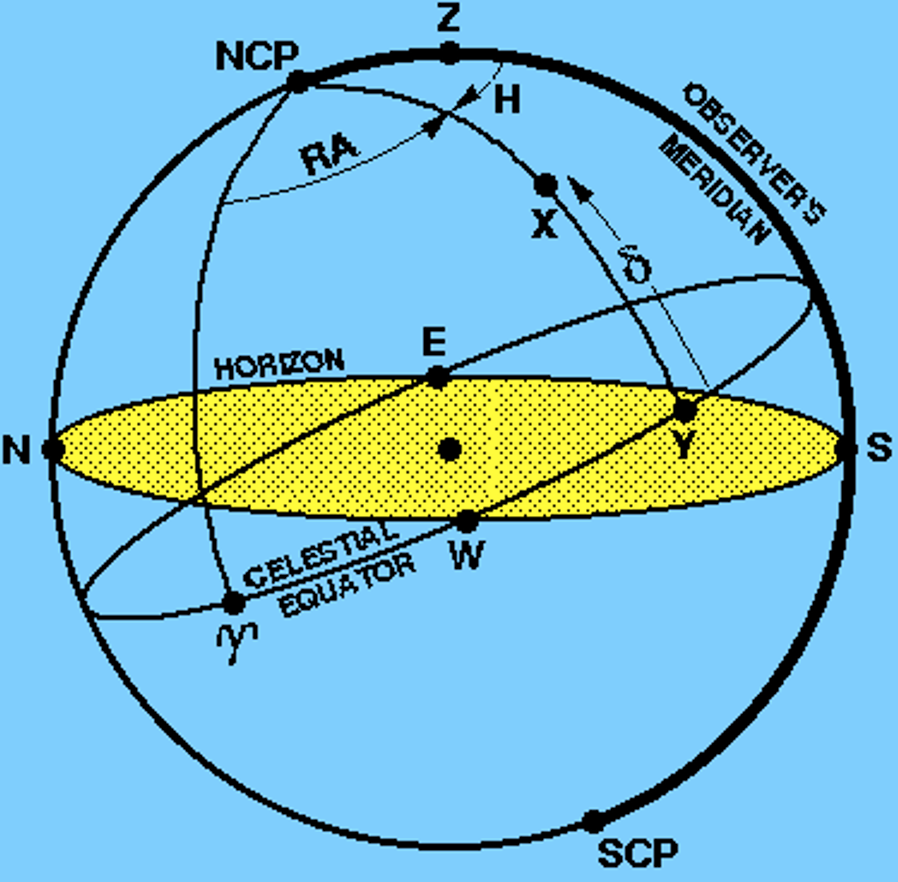
\includegraphics[width=5 cm]{Coordinate equatoriali.png}
\end{figure}
Dobbiamo però sapere però come cambiare dalle coordinate equatoriali a quelle altazimutali. Avevamo definito l'angolo orario come la distanza angolare rispetto a Greenwich, l'angolo orario fra il punto $\gamma$ e il meridiano di Greenwich viene definito come \textbf{tempo siderale} $ST$. Il tempo siderale è l'ascensione retta degli oggetti che stanno al meridiano.
$$H=ST-\alpha$$
Questo ci permette facilmente di capire dove puntare il telescopio. In questo modo si possono creare delle mappe di cielo con ascensione retta e declinazione.\\
Tutto questo si basa sull'inclinazione dell'asse terrestre rispetto al piano orbitale, abbiamo supposto che questa rimanga costante ma non è così, infatti la Terra come una trottola precede. Il periodo di \textbf{precessione} è molto lungo (non umano) 25772 anni, sembrerebbe che non sia un problema ma in realtà lo è se si vuole una grande precisione. L'asse ora punta alla Polare prima puntava su altre stelle. A questo effetto di precessione si somma il movimento di \textbf{nutazione} dovuto alla presenza della Luna.
\begin{figure}[ht]
    \centering
    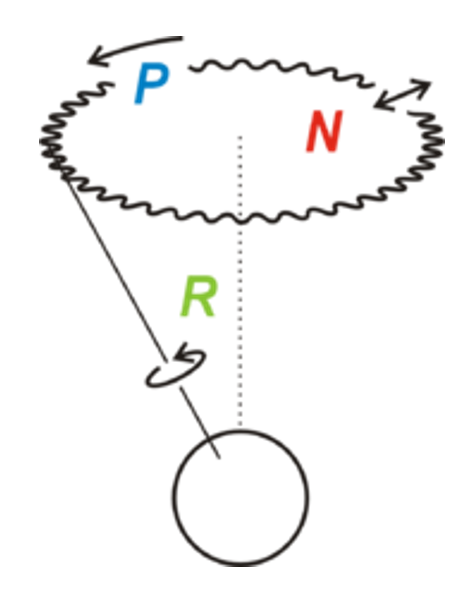
\includegraphics[width=5 cm]{precessione e nutazione.png}
\end{figure}
Questo periodo è troppo lungo per essere ignorato? Facciamo una proporzione
$$\frac{2\pi}{25772\ yr}=\frac{2\pi}{25772\cdot 365.25\ d}=6.67\cdot 10^{-7}\ \text{rad/day}$$
Cioè le stelle si spostano ogni giorno di $6.67\cdot 10^{-7}$ radianti.\\
In astronomia radianti e gradi sono troppo grandi, si preferisce utilizzare delle unità di misura legate al tempo, l'ascensione retta è misurata in ore minuti e secondi, è legato alla tradizione marinaresca, era più facile costruire buoni orologi piuttosto che buoni goniometri. In astronomia si usano gli arcominuti $[']$ e gli arcosecondi $['']$.
$$1\text{ arcmin}=\frac{1^\circ}{60}\qquad 1 \arcsec =\frac{1'}{60}=\frac{1^\circ}{3600}$$
Convertiamo gli arcosecondi in radianti
$$1 \arcsec =\frac{1^\circ}{3600}=\frac{2\pi}{360\cdot3600}=4.848137\cdot 10^{-6}\ \text{rad}$$
Quindi 
$$1\text{rad}=206264.8062''$$
La precessione in arcosecondi è di $0.13''$ al giorno.
Per dare una idea di cosa è un arcosecondo, una stella a livello del mare è grande $5''$, in montagna $2''$ pertanto la precessione è importante, dopo un anno bisogna tener conto della precessione, possiamo sbagliare stella fda puntare se non ne teniamo conto.\\
Un altro effetto da tenere conto è l'atmosfera terrestre che fa rifrangere la luce, quindi gli oggetti cambiano di posizione con l'altezza. La rifrazione dipende con la distanza zenitale, una stella può apparire $30''$ in un posto diverso.\\
Esiste un sistema di riferimento internazionale centrato nel Sole e i tre assi sono definiti con gli oggetti più lontani che conosciamo perché si suppone che più un oggetto è lontano meno lo vedremo muovere, la distanza apparente è minore. Il sistema di riferimento è chiamato \textbf{International Celestial Reference System}(ICRS) è stato deciso dalla International Astronomical Union (IAU). Abbiamo cataloghi con migliaia di oggetti con le loro coordinate. Il database più grande si trova sul sito \textit{simbad}.

\newpage
\section{Lezione del 7/10}
\subsection{La radiazione elettromagnetica}
Fin'ora abbiamo parlato di astronomia, studiando il cielo per scopi principalmente civili, senza applicare la fisica ai corpi celesti presi in considerazione. \\
Per comprendere la natura di un oggetto celeste, dobbiamo prima chiederci quali siano le proprietà del vettore che trasporta le uniche informazioni che abbiamo a disposizione su tale oggetto: la luce da esso emessa e, quindi, la natura della radiazione elettromagnetica.\\
In questo studio, il parametro più importante è proprio il campo elettrico dell'onda perché 
\begin{enumerate}
    \item è facilmente misurabile (diversamente dal campo magnetico);
    \item ci consente di studiare la sorgente che lo ha emesso, essendo la radiazione una variazione nello spazio di tale campo.
\end{enumerate} 

Ricordiamo che, per un'onda e.m. la frequenza è legata alla lunghezza d'onda secondo la relazione $$ c = {\lambda}{\nu}$$ ed essendo la velocità della luce \(c\) una costante universale, possiamo considerare tali grandezze come equivalenti.
\\ In che modo il campo elettrico di un'onda e.m. può fornirci informazioni? Posizionando un sensore in un certo punto dello spazio, questo vedrà il campo variare in quel punto in diversi modi (sempre secondo una legge sinusoidale) a seconda della polarizzazione dell'onda:  ad esempio, se la polarizzazione dell'onda è \textit{lineare} (cioè, il vettore campo elettrico mantiene la sua direzione di propagazione costante nel tempo), il sensore vedrà oscillare il campo elettrico seguendo un moto armonico in un piano perpendicolare alla direzione di propagazione dell'onda
\begin{figure}[h!!]
    \centering
    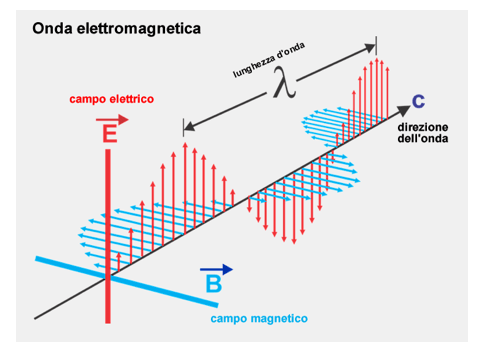
\includegraphics[width=5cm]{onda-elettromagnetica.png}
    \label{fig:my_label1}
\end{figure}

mentre se la polarizzazione è \textit{circolare}, il vettore si muoverà di moto circolare uniforme nello stesso piano. 

\begin{figure}[h!!]
    \centering
    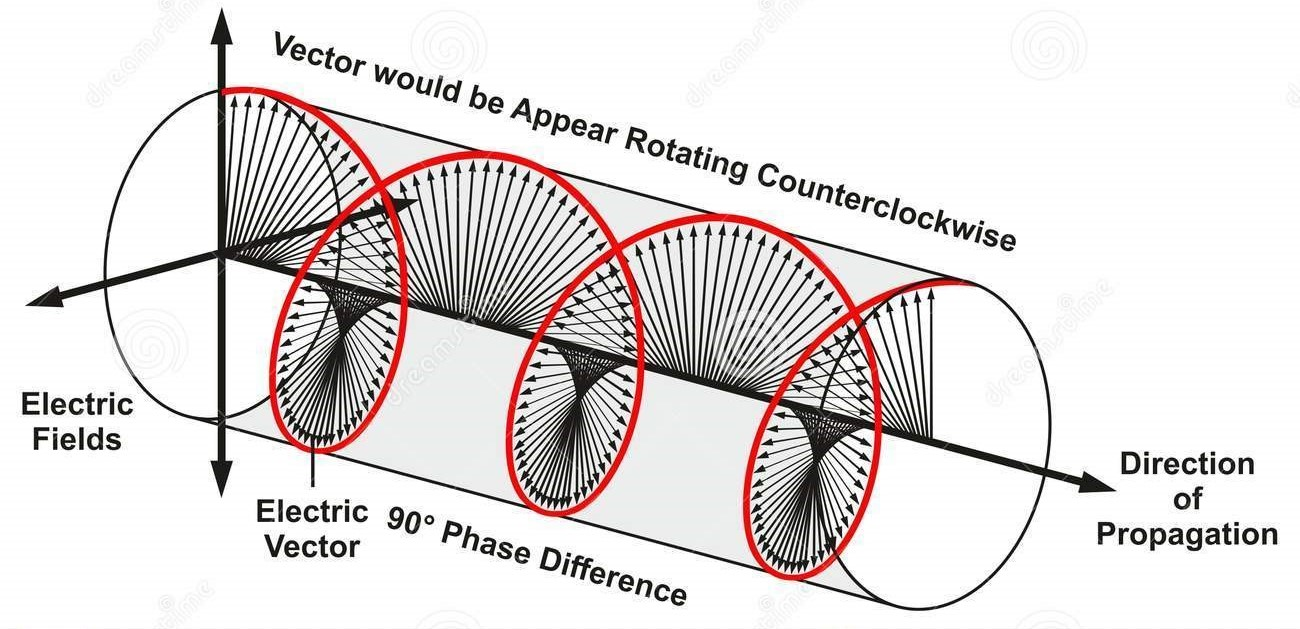
\includegraphics[width=5cm]{pol circ.jpg}
    \label{fig:my_label2}
\end{figure}

Il sensore interpreta queste variazioni e le converte in segnali attraverso opportuni processi. \bigskip\\


N.B: per frequneze nell'ordine di grandezza della luce visibile non esistono ancora sensori in grado di rilevare con precisione la fase della radiazione luminosa perché troppo piccola (varia nell' o.d.g. di \(10^{15}\)); è per questo motivo che nello studio di queste onde consideriamo solo i valori medi di tali grandezze, operando un integrale sulla parte temporale dell'equazione dell'onda ed osservando così le sole variazioni spaziali del campo elettrico.\smallskip\\

La radiazione prende un nome a seconda della lunghezza d'onda da essa posseduta. Nell'immagine seguente, sono riportate le tipologie di radiazioni principali e i relativi intervalli di lunghezza d'onda (e frequenza) entro cui ricadono: 
\begin{figure}[h!!]
    \centering
    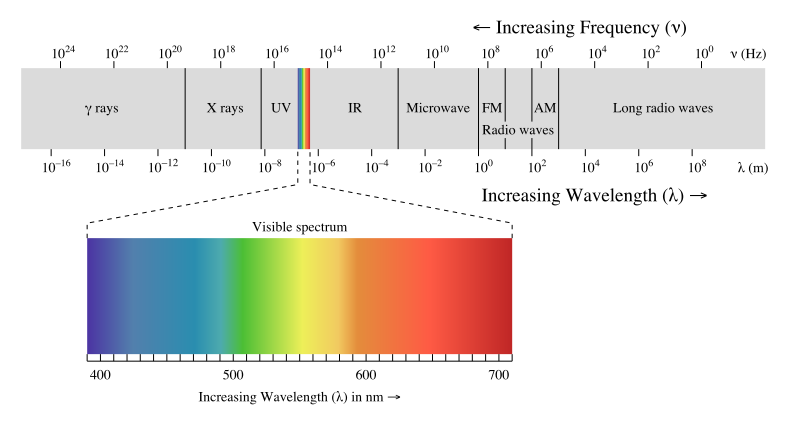
\includegraphics[width=10cm]{spettro em.png}
    \label{fig:my_label3}
\end{figure}

Di tutto ciò che potrebbe essere potenzialmente emesso da una sorgente sotto forma di onda e.m., l'occhio umano vede solo quella parte che va dai \(400nm\)  ai \(700nm\), che prende il nome di \textit{luce visibile}. \\
Vorremo ora quantificare l'energia trasportata da ognuna delle singole lunghezze d'onda, ovvero l'energia associata ad una specifica radiazione. Tale analisi quantitativa fu condotta per la prima volta alla fine del 1700 da Sir William Herschel, astronomo che misurò il primo spettro solare della storia. Scomponendo, infatti, la luce solare in diversi colori attraverso l'uso di un prisma, Sir Herschel pose un termometro su ogni colore e ne misurò la temperatura (esprimente una forma di energia) in funzione della lunghezza d'onda del colore.
Inoltre, posizionando un termometro \textit{vicino} al colore rosso (ma non sulla parte di piano illuminata da esso), si accorse che anche questo si riscaldava e, quindi, intuì l'esistenza della radiazione "infrarossa" (intendendo un'onda con frequenza superiore a quella del rosso, non visibile all'occhio umano). \\

In astrofisica, per quantificare l'energia usiamo una grandezza detta \textbf{Intensità specifica} per unità di lunghezza d'onda, ovvero la quantità di energia che attraversa una superficie infinitesima data quella particolare \(\lambda\):
\begin{equation*}  
    I_{\lambda}(\theta,\phi)d\lambda = \frac{dE_{\lambda}d\lambda}{dtdA\cos{\theta}d\omega}
\end{equation*} \\

La precedente definizione d'intensità specifica normalizza l'energia nell'unità di tempo \(dt\) e tiene anche conto dell'orientamento della superficie rispetto alla direzione di propagazione dell'onda incidente: quindi, non si normalizza tanto per l'area infinitesima \(dA\), quanto per l'area proiettata lungo la direzione di propagazione dell'onda \(dA\cos{\theta} \). Infine, è necessario anche tenere conto dell'estensione  della superficie soggetta alla radiazione e, quindi, dell'angolo solido \(d\omega\) con cui la sorgente puntiforme vede la superficie. Si può anche dare la stessa definizione di Intensità specifica per unità di frequenza:
\begin{equation*}
    I_{\nu}(\theta,\phi)d\nu = \frac{dE_{\nu}d\nu}{dtdA\cos{\theta}d\omega}
\end{equation*} \\


Una importante proprietà dell'intensità specifica afferma che questa grandezza \textit{non dipende dalla distanza}. Consideriamo  infatti due superfici, \(dA\) e \(dA'\) molto distanti tra loro, e gli angoli con cui una superficie vede l'altra ( \(\theta\) e \(\theta'\)). 
\begin{figure}[h!!]
    \centering
    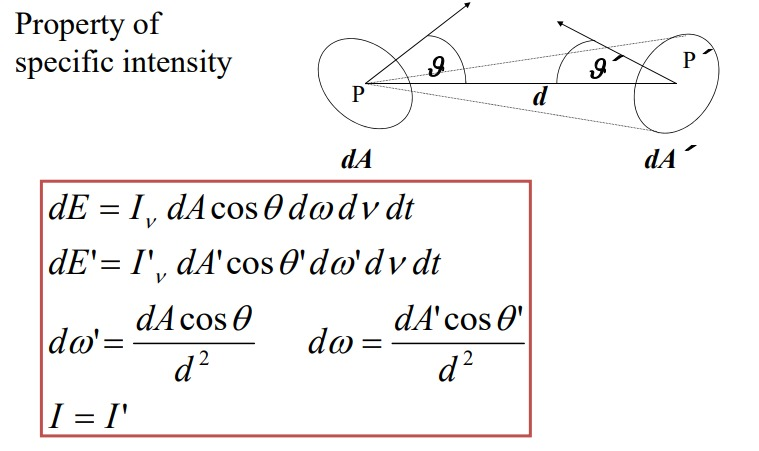
\includegraphics[width=5cm]{WhatsApp Image 2023-01-08 at 10.41.49.jpeg}
    \label{fig:my_label3}
\end{figure}
Essendo \(dA\cos{\theta} \) e \(dA'\cos{\theta'} \) le proiezioni di due superfici infinitesime sulla medesima direzione (quella individuata dalla congiungente), queste due quantità possono essere considerate uguali e, ricordando la definizione di angolo solido \(d\omega\), si giunge alla conclusione che \textit{l'intensità specifica della radiazione incidente su entrambe \(dA\) e \(dA'\) è la stessa}, cioè è indipendente dalle distanze e dipende solo dagli angoli con cui le due superfici si guardano.\\
N.B. Questo solo se non sono presenti altre sorgenti o corpi assorbenti nello spazio compreso tra \(dA\) e \(dA'\).\\

Questo significa che, ad esempio, l'intensità specifica della radiazione solare che emerge da una porzione di superficie del sole è la stessa di quella che arriva ad un telescopio sulla Terra che guarda quella stessa porzione di superficie.\\


Quello che gli astronomi misurano nella pratica con i loro strumenti è la \textbf{luminosità} del corpo celeste 
\begin{equation*}
    L = \frac{dE}{dt}
\end{equation*}
cioè la quantità di energia della radiazione incidente nell'unità di tempo.   
Inoltre, approssimando le sorgenti ad oggetti puntiformi, si vede che l'intensità luminosa dell'onda diminuisce nello spazio come la superficie di una sfera di raggio pari alla distanza \(d\) dalla sorgente. Questa considerazione porta alla definizione di \textbf{flusso} di una sorgente a distanza \(d\): 
\begin{equation*}
    S = \frac{L}{4\pi d^2}
\end{equation*}
che ci permette di legare la luminosità che misuriamo con i telescopi alla sorgente emettitrice.\\
Se le sorgenti piuttosto che essere puntiformi avessero delle dimensioni non trascurabili, la luminosità e il flusso diventerebbero funzioni delle coordinate del punto della sorgente preso in considerazione. Definiamo, infine, la \textbf{brillanza superficiale} di una sorgente estesa come la \textit{somma} di tutti i possibili contributi al flusso dati dai vari punti della superficie della sorgente. 


\subsection{Tecniche astronomiche: fotometria}

Il primo metodo di classificazione delle stelle fu introdotto da Ipparco nel 129 AC, che immaginò di dividerle in 6 grandezze: le più brillanti le definì di \textit{prima magnitudine}, mentre le meno brillanti all'occhio umano \textit{di sesta magnitudine.}\\
Pogson fu il primo però, nel 1856, a quantificare in maniera oggettiva il sistema di magnitudine di Ipparco. Osservò, infatti, che una stella di prima magnitudine produceva 100 volte più luce di una stella di sesta magnitudine e che, dunque, \textit{la scala introdotta da Ipparco non era affatto lineare}. Oggi noi sappiamo che il motivo risiede nel fatto che l'occhio umano non percepisce linearmente l'aumento di luminosità di una sorgente (cioè, non sempre in corrispondenza di una variazione del numero di fotoni emessi, noi riusciamo a percepire la stessa variazione di intensità).\\
Pogson stabilì che una differenza di 5 magnitudini tra due stelle corrispondesse esattamente al rapporto di 100:1 in brillanza e che, quindi, \textit{una magnitudine di differenza corrispondesse alla radice quinta di 100, cioè circa 2.5}.
Allora, la scala (adatta al sistema di Ipparco) da usare per esprimere la differenza in magnitudine tra due stelle è una \textit{scala logaritmica in base 10}, che adotta come coefficiente 2.5 (corrispondente a quanto equivale una magnitudine in brillanza).\\ 
Per cui la magnitudine di Ipparco ci può riportare al flusso (o alla brillanza) e viceversa (operando, quindi, una conversione) in relazione sempre ad una magnitudine di riferimento \(m_0\), secondo l'equazione: 
\begin{equation}
   m = m_0 - 2.5\log_{10}(F)
\end{equation}
Secondo la (1), più è piccola la magnitudine, più l'oggetto è luminoso rispetto all'altro.\\ 
Nella scala di Ipparco, l'oggetto più luminoso visibile ad occhio nudo ha magnitudine zero ed è Vega. Poi, sempre tra quelli che vediamo ad occhio nudo, quello meno brillante ha magnitudine 6 \textit{rispetto a Vega}. Essendo una scala logaritmica, è possibile anche introdurre valori negativi: il sole, ad esempio, ha magnitudine \(-26\) rispetto a Vega. Cosa vuol dire? Operando l'equazione (1): \(-26 = 0 -2.5\log_{10}(F)\) e quindi \(F = 10^{10}\); significa che la differenza di flusso tra Vega (oggetto a magnitudine zero) ed il sole è di \(10^{10}\). Secondo questa scala, dunque, gli oggetti meno luminosi hanno magnitudine positiva e quello meno luminoso mai misurato possiede una magnitudine di \(+30\), il che significa che per condurre misurazioni ci servono strumenti in grado di osservare range di brillantezza dell'ordine di \(10^{22}\).\\
Una magnitudine così definita dunque ci dice quanto è luminoso un oggetto rispetto ad un altro, ma non dice nulla sua luminosità intrinseca ed è detta per questo \textbf{Magnitudine apparente}.  Viene allora introdotta la \textbf{Magnitudine assoluta}.\\
Ricordando che il flusso rende conto della diminuzione della luminosità in funzione della distanza secondo la legge 
\begin{equation*}
    F = \frac{L}{4\pi d^2}
\end{equation*}
potremmo idealmente ricollocare tutti gli oggetti da confrontare alla medesima distanza e chiederci quale sia veramente il più luminoso (in senso assoluto). Ad esmepio, il Sole è più luminoso rispetto a Vega, ma solo perché è più vicino alla Terra. E se li collocassimo entrambi alla stessa distanza, quale dei due sarebbe ora il più luminoso?\\ 
La magnitudine assoluta, viene definita allora come la magnitudine apparente di una sorgente posta ad una distanza di \(10 pc\) dall'osservatore.  
Quindi, la definizione della magnitudine assoluta di una stella corrisponde concettualmente al riportare tutte le stelle alla stessa distanza che, per convenzione, si decide essere pari a \(10 Parsec\) (dove \(1pc = 3.086 10^{16} \) metri).


\subsection{Telescopi}
Analizziamo ora le caratteristiche dello strumento che ci permette di misurare i fotoni (e, quindi, la luce) emessi da una stella che desideriamo studiare: il telescopio.
Il compito dei telescopi è quello di raccogliere la radiazione che arriva dallo spazio e riunirla in un unico punto. La storia ci dice che Galileo non inventò il telescopio, ma che comunque fu il primo ad utilizzarlo per condurre misure astronomiche.\\ 
Se decidessimo di graficare un istogramma del numero di fotoni che arrivano su un determinato telescopio in ogni intervallo di tempo, ci accorgeremmo subito che la statistica che domina questo fenomeno è la \textit{Statistica di Poisson}.
Questa afferma che per \(N\) eventi indipendenti (in questo caso, l'arrivo di un fotone) in un dato intervallo di tempo, la probabilità di osservarne \(n\) è di 
\begin{equation*}
    P_N(n) = \frac{N^n}{n!}e^{-N}.
\end{equation*}
Allora, se \(N\) è il valore medio del numero di fotoni che sono arrivati sul nostro telescopio, l'errore su questo conteggio, secondo Poisson è dato dalla radice quadrata della media: \(\sqrt{N}\). 
L'errore relativo sarà, quindi, \(\frac{\sqrt{N}}{N} = \frac{1}{\sqrt{N}}\). 
Gli astrofisici preferiscono comunque calcolare la qualità della misura come l'inverso dell'errore relativo, frazione che corrisponde al cosiddetto \textbf{rapporto segnale su rumore}:
\begin{equation*}
    \frac{Signal}{Noise} = \sqrt{N}.
\end{equation*}\\
Il telescopio costruito da Galielo, detto \textit{rifrattore}, si basava sull'utilizzo di due lenti di vetro: la lente primaria , convergente, aveva il compito di raccogliere i raggi del fronte d'onda piano incidente e convogliarli vero il fuoco, formando un'immagine puntiforme; la seconda lente, detta oculare e divergente, ritrasformava l'immagine puntiforme in un fronte d'onda piano che poteva essere visto dall'occhio. 
L'utilità della prima lente stava nel raccogliere molti più fotoni rispetto alla quantità di cui sarebbe stato capace l'occhio umano da solo. Veniva così amplificato il segnale di una stella. 
\begin{figure}[h!!]
    \centering
    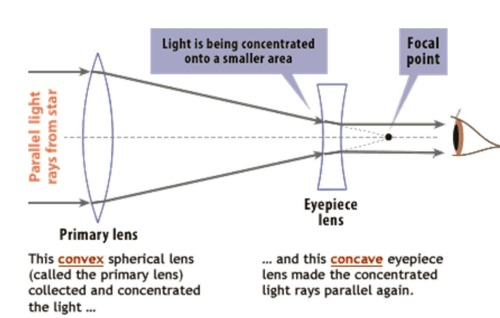
\includegraphics[width=5cm]{WhatsApp Image 2023-01-09 at 02.42.01.jpeg}
    \label{fig:my_label4}
\end{figure}\\
Il telescopio proposto da Newton, detto \textit{riflettore}, invece usava uno specchio ricurvo per convogliare i raggi di luce verso un secondo specchio, inclinato di 45 gradi rispetto alla focale, che li rifletteva tutti in un punto ben preciso.
\begin{figure}[h!!]
    \centering
    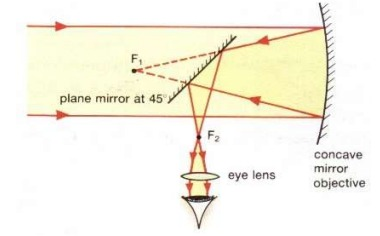
\includegraphics[width=5cm]{WhatsApp Image 2023-01-09 at 02.44.03.jpeg}
    \label{fig:my_label5}
\end{figure}\\
In ogni caso, ciò che  caratterizza un telescopio è il diametro \(D\) del suo  specchio primario; infatti, il numero di fotoni \(N\) raccolti da un telescopio è proporzionale all'area di tale specchio e, quindi, a \(D^2\). Allora, se il rapporto segnale rumore è \(\frac{Signal}{Noise} = \sqrt{N}\) e \(N \propto D^2\), il rapporto segnale rumore va con il diametro \(\frac{signal}{noise} \propto D\). Per cui, raddoppiare il diametro significa raddoppiare la qualità della misura. 
Alternativamente, se si vuole migliorare la qualità della misura avendo un diametro fisso, essendo \(N \propto T_{exp}\), si può pensare di esporre il telescopio più a lungo alla sorgente luminosa, aumentando il numero di fotoni cosi rivelati. Ovviamente, più è grande il diametro, meno tempo si impiegherà a raccogliere il numero N di fotoni desiderato. 
\newpage

\subsubsection{Proprietà di un telescopio}

Le caratteristiche di un sistema ottico utili per descrivere un telescopio sono elencate nella seguente figura:
 \begin{figure}[h!!]
    \centering
    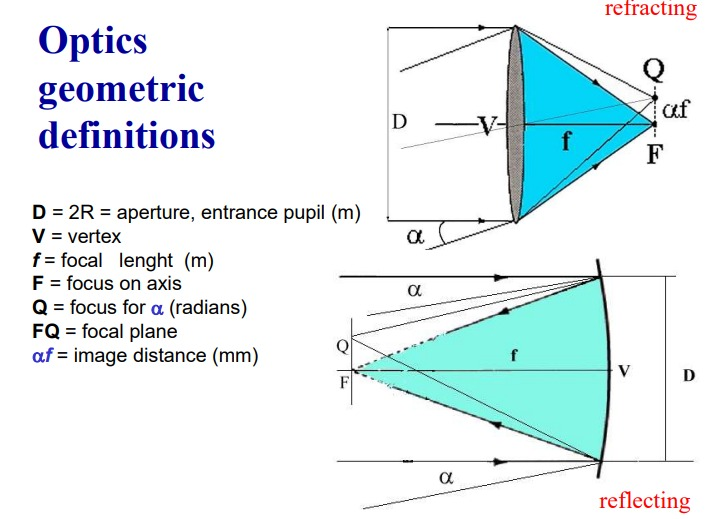
\includegraphics[width=8cm]{WhatsApp Image 2023-01-09 at 02.46.32.jpeg}
    \label{fig:my_label6}
\end{figure}\\
Il fuoco, in particolare, rappresenta il punto sull'asse ottico in cui tutti i raggi incidenti paralleli all'asse ottico vengono convogliati dalla lente o dallo specchio del telescopio. Nel caso in cui, i raggi incidenti dell'oggetto  osservato siano inclinati di un certo angolo \(\alpha\) rispetto alla direzione dell'asse ottico, l'immagine si formerà in un punto Q (diverso dal fuoco) giacente sul cosiddetto \textbf{piano focale} e distante dal fuoco \(f\sin{\alpha} \simeq f\alpha\). Questa distanza corrisponde anche alla distanza della sorgente dall'asse focale.
Quanto sarà grande il piano focale? Il fattore di scala di questo piano sarà dato da un radiante espresso in arcosecondi diviso la focale espressa in millimetri, cioè 
\begin{equation*}
    \frac{206264.8062''}{f}
\end{equation*}\\
Quindi, ad esempio, se il mio telescopio ha una focale di 16 metri, una stella diampiezza 1 arcosecondo sarà grande su questo telescopio \(0.388 mm\).\\
Allora, se per il diametro del telescopio è facile affermare in generale che più grande è e meglio è, per la focale la grandezza va decisa in base alle misure che lo sperimentatore vuole condurre (di una singola stella come della luna), poiché cambierà il modo in cui gli oggetti verranno visualizzati.\\
Il \textbf{campo di vista} è la quantità di cielo che un telescopio può osservare contemporaneamente. Quantitativamente, è l'angolo \(\phi\) che il "raggio principale" (cioè quel raggio che si propaga attraverso la lente senza essere rifratto) può sottendere data l'apertura dell'oculare da cui l'occhio osserva l'immagine. I telescopi moderni hanno un campo di vista nell'ordine degli arcominuti. 
 \begin{figure}[h!!]
    \centering
    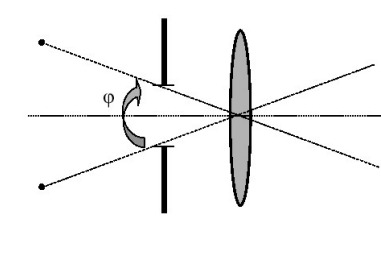
\includegraphics[width=5cm]{WhatsApp Image 2023-01-09 at 02.51.58.jpeg}
    \label{fig:my_label7}
\end{figure}\\
La \textbf{potere risolutivo} è l'abilità di un telescopio di separare due ogetti, ad esempio due stelle in cielo che distano l'una dall'altra di un certo angolo. L'angolo di distanza più piccolo a cui il telescopio riesce a distinguere due oggetti è detto \textbf{risoluzione angolare}.
Per capire cosa sia davvero il potere risolutivo analizziamo l'esperimento della doppia fenditura.\\
Quando una radiazione e.m. incide sulla piccola fenditura che è l'apertura del telescopio, secondo il principio di Huygens, ogni punto della fenditura stessa diventa una nuova sorgente di fronte d'onda circolare. Questi fronti si sovrappongono a formare una nuova onda risultante che può essere descritta come la trasfromata di Fourier del prodotto delle funzioni \(E(x,t) = E_0e^{i(kx-\omega t)}\), espressione dell'onda piana incidente, e la funzione di trasmissione del telescopio definita a tratti come \(G(x) = 1 \) se\(x\) individua un punto dentro l'apertura e \(G(x) = 0 \) altrimenti. 
\begin{figure}[h!!]
    \centering
    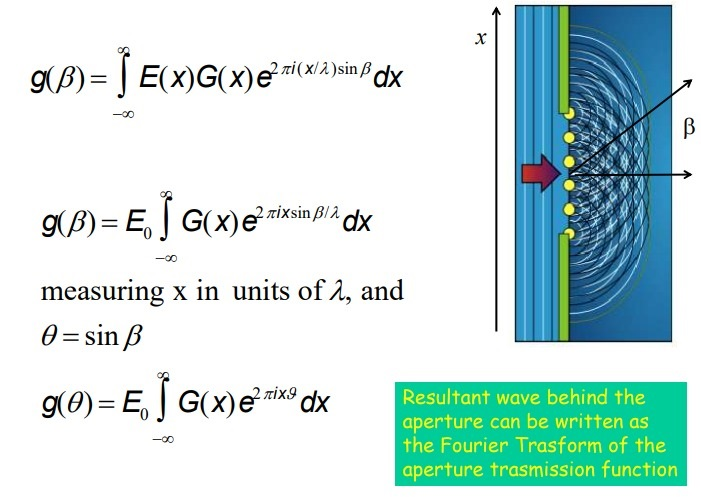
\includegraphics[width=10cm]{WhatsApp Image 2023-01-09 at 02.55.01.jpeg}
    \label{fig:my_label8}
\end{figure}\\
Questa nuova funzione ci darà il valore dell'onda in una qualunque direzione descritta dalla coordinata spaziale \(\beta\) o dalla coordinata angolare \(\theta\).\\
Svolgendo l'integrale della trasformata di Fourier espressa in funzione dell'angolo, si ottiene la funzione seno circolare
\begin{equation*}
    g(\theta) = E_0 \int_{-\infty}^{+\infty} G(x)e^{2ix\pi\theta},dx = E_0 \frac{sin(\pi t)}{\pi t}
\end{equation*}\\
Il grafico di tale integrale sarà 
\begin{figure}[h!!]
    \centering
    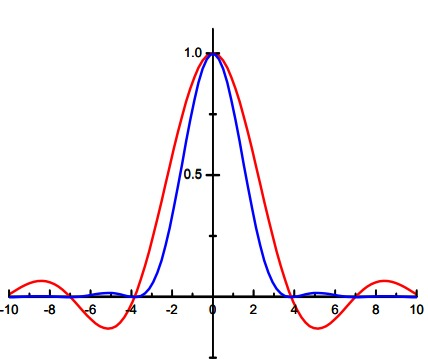
\includegraphics[width=5cm]{WhatsApp Image 2023-01-09 at 02.57.58.jpeg}
    \label{fig:my_label9}
\end{figure}\\
Si giunge alla conclusione che al centro della fenditura ci sarà molta luce; allontanandoci da essa, la luce sarà meno intensa fino a che spunteranno altri picchi luminosi (anche questi meno intensi del picco principale) in corrispondenza di precisi punti.\\
Considerando che l'apertura del telescopio non è una semplice striscia, ma presenta una forma circolare l'immagine che si otterrà, detta \textbf{the Airy function} e descritta dalla funzione di Bessell, è la seguente:
\begin{figure}[h!!]
    \centering
    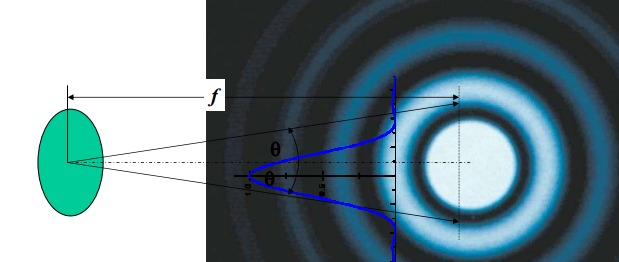
\includegraphics[width=5cm]{WhatsApp Image 2023-01-09 at 02.59.37.jpeg}
    \label{fig:my_label10}
\end{figure}\\
Si dimostra che il picco dello spettro (il centro, corrispondente alla parte più luminosa) si allinea con il centro dell'apertura circolare del telescopio quanto più è grande il diametro D del telescopio stesso. Infatti, chiamando \(\theta\) l'angolo di distanza tra i due centri (vedi figura sopra) si ha \(\sin{\theta} = \frac{1.22\lambda}{D}\) per il primo picco. Più cresce D, più il seno tenderà a zero e, quindi, più teta sarà approssimabile a zero (sovrapposizione). Per cui, più un telescopio è grande più mi aspetto che la larghezza dello spettro prodotto da una stella sia piccola.\\
Immaginiamo, ora, di osservare due stelle molto vicine. I due spettri prodotti da esse (considerando che presentano una certa larghezza) potrebbero sovrapporsi, per cui è lecito chiedersi in che condizioni il telescopio riuscirà a distinguere le due stelle. Se la separazione dei picchi dipende dal risoluzione angolare \(\phi\) del telescopio, il diametro del telescopio determinerà invece quanto le larghezze dei due spettri saranno grandi e, quindi, quanto essi si sovrapporranno o meno.  Il \textbf{criterio di Reileigh} stabilisce una condizione ogettiva: due sorgenti si potranno ritenere distinte se lo zero della prima sorgente cade sul massimo della seconda sorgente.  (\textit{consiglio di leggere la parte sul criterio di Reileigh dalle slide di Costa, spiegata molto meglio})\\
Nel paragrafo precedente abbiamo descritto due modelli di telescopi: il rifrattore di Galilei e il riflettore di Newton. Nell'uso pratico, entrambi presentarono diversi problemi che, nel tempo, furono più o meno risolti dagli astronomi. Ne vediamo di seguito i principali per le due tipologie. 

\subsubsection{I problemi dei rifrattori}
 \begin{enumerate}
\item Le lenti usate hanno un \textit{fuoco che dipende dalla lunghezza d'onda} e questo costituisce il fenomeno della cosiddetta \textbf{aberrazione cromatica}: supponiamo, allora, di voler osservare una stella di luce policromatica: sull'asse del telescopio si formeranno tante immagini monocromatiche della sorgente quanti sono i colori della sorgente stessa, in punti diversi dell'asse ottico (i diversi fuochi, ognuno corrispondente ad una lunghezza d'onda). Non avremo, dunque, un'unica immagine complessiva.
Si risolse in parte il problema usando \textit{lenti acromatiche}, cioè lenti secondarie che hanno l'obiettivo di spostare il fuoco di alcune lunghezze d'onda di una data quantità, in modo da far coincidere tutti i fuochi della lente del telescopio in un unico punto e formare un unica immagine.


\item Maggiore è l'area della lente (ciò che idealmente vorremmo sempre, perchè un telescopio più grande equivale a misure migliori), maggiore è il suo spessore. Dunque, aumenta il rischio che vi siano fenomeni di\textbf{assorbimento}  della radiazione durante il suo passaggio attraverso la lente. 


\item I rifrattori erano soliti avere delle focali molto lunghe per evitare il problema della distorsione dell'immagine in una direzione; infatti, imperfezioni nella lavorazione della lente facevano sì che non tutti i raggi rifratti si concentrassero esattamente in corrispondenza del fuoco, facendo apparire l'immagine un po' allungata. Tuttavia, in questo modo il telescopio risultava eccessivamente grande e difficile da maneggiare.
 \end{enumerate}

\subsubsection{I problemi dei riflettori}
\begin{itemize}

\item I primi riflettori furono delle sfere perché facili da realizzare. Purtroppo però, per una sfera riflettente è sempre soggetta al problema dell'\textbf{aberrazione sferica}. Questo consiste nell'inesistenza di un vero e proprio fuoco per questo tipo di telescopi, a causa del fatto che la posizione in cui viene riflesso un certo raggio (incidente parallelamente all'asse ottico) dipende dalla distanza del punto di incidenza del raggio dal vertice dello specchio. I vari raggi verranno riflessi in punti diversi dell'asse. 
Di conseguenza, non esiste per essi un punto in cui la sorgente diventi esattamente puntiforme; piuttosto, l'immagine è sempre vista come un punto con intorno un certo anello circolare concentrico al punto, più o meno largo. Il meglio che si possa fare è di individuare e osservare la sorgente luminosa nella posizione in cui l'anello presenta il diametro minore (\textit{cerchio di minima confusione}).


\item La forma perfetta che permette, al contrario della sfera, di raccogliere in un unico punto (fuoco) i raggi provenienti dall'infinito è il paraboloide. Anche questo telescopio presenta un problema: nel caso in cui i raggi non incidano parallelamente all'asse ottico, il fuoco sarà un oggetto esteso e non più puntiforme. Allora, l'immagine di una stella non collocata sull'asse del telescopio sarà allungata in una direzione. Si parla di \textbf{Coma}.



\item Un altro difetto è \textbf{l'astigmatismo}. I telescopi, infatti, idealmente prevederebbero una perfetta simmetria assiale dell'occhio umano (l'occhio vede una certa figura alla stessa maniera comunque essa venga ruotata), cosa che in realtà non succede mai.  Le immagini risultano allora allungate in  una direzione. Questo problema si risolve con delle lenti sferiche, che permettono all'imagine di allungarsi o schiacciarsi in una direzione ben precisa. 
\end{itemize}
Nonostante queste complicanze, nel tempo i riflessori furono preferiti ai rifrattori.
\newpage
\section{Lezione del 10/10}

\subsection{Le varie tipologie di telescopi}
I telescopi sono strumenti in grado di raccogliere i fotoni che arrivano distribuiti nello spazio in un punto detto "fuoco" (di un’ottica che può essere sia un rifrattore che un riflettore) e sono in grado di aumentare la nostra capacità di vedere oggetti angolarmente piccoli (per piccoli non si intende un oggetto di una data lunghezza, ma piuttosto di una grandezza, di una dimensione angolare).
Abbiamo visto che la capacità di raccogliere fotoni va con l’apertura (diametro) del telescopio al quadrato ($D^2$), mentre il potere risolutivo va con il diametro (quindi se raddoppiamo il diametro del telescopio abbiamo 4 volte più fotoni e 2 volte più risoluzione angolare).

Abbiamo visto che i telescopi devono essere degli oggetti fisici ed essi hanno difetti tipici dell’ottica: alcuni sono legati alla forma (che quindi può essere quantomeno corretta); altri, come il coma, sono invece semplicemente legati al fatto che possono osservare in maniera ottimale ciò che è sull’asse del telescopio, ma magari hanno dei difetti quando si guardano oggetti fuori dall’asse del telescopio. Ma qual è la grandezza dei difetti di cui parliamo? Per dare un’idea di quali numeri sono in gioco, quando volò lo Space Telescope ci fu un problema poiché le immagini non avevano la qualità ottica desiderata: in pratica lo specchio dello Space Telescope, che è dell’ordine di 2,5 metri, era stato lavorato male e quindi non vedeva così bene come si voleva. Fu fatta una missione spaziale per correggere questo difetto ottico.

Come avere immagini di buona qualità? Abbiamo detto che il telescopio dovrebbe essere più una parabola: questa parabola era sostanzialmente 2,5 micron più schiacciata di quella che avrebbe dovuto essere, quindi un errore di 2,5 micron porta ad una immagine di qualità non utile per l’osservazione (questo per darvi un'idea con che precisione bisogna fare i disegni e con che precisione bisogna lavorare per l'ottica).

I telescopi possono essere fatti con oggetti molto diversi tra di loro. Una configurazione di telescopio prevede che i raggi che provengono dalla sorgente convergono nel fuoco che prende il nome di “primo fuoco”. Ora, se noi costruiamo telescopi di questo genere, il primo fuoco del telescopio, che si trova tra la sorgente e lo specchio, deve essere occupato da uno strumento.
\begin{figure}[h!!]
        \centering
        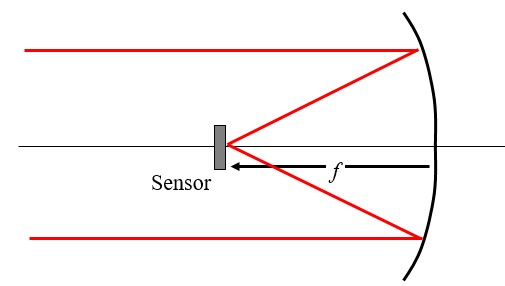
\includegraphics[width=9cm]{1.jpg}
        \label{}
    \end{figure}
\\Qui, al primo fuoco, è stato sospeso uno strumento sul quale si posizionavano delle lastre fotografiche. 
Ora è chiaro che questo tipo di configurazione ottica non è ottimale per il semplice motivo che non posso avere uno strumento molto grande (perché se io ho un telescopio di 1 metro, come quello di Serra La Nave, e mi metto io, questo strumento non può essere allocato, perché farebbe ombra) e in più se noi usassimo solo il primo fuoco avremmo una focale corta, cioè la distanza tra lo specchio e il fuoco non potrebbe essere ovviamente nulla, perché altrimenti lo strumento dovrebbe essere esteso (per esempio, se ho uno specchio di 1 metro, difficilmente potrò avere una focale più di 3 metri, altrimenti devo costruire un telescopio alto come un palazzo e questo potrebbe avere altri tipi di problemi). Ricordiamo che la focale corta significa una proiezione sul piano focale molto piccola.
A questo punto la configurazione è stata completata ed ecco qui che entra in gioco la configurazione “Cassegrain Telescope” (ci sono tante configurazioni, io vi mostro le più usate).
\begin{figure}[h!!]
        \centering
        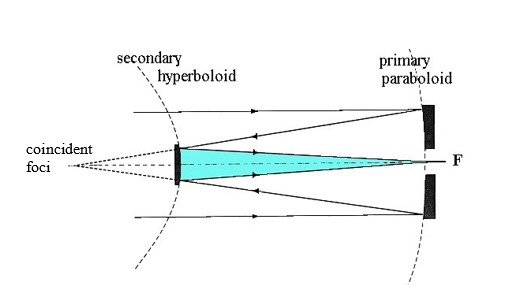
\includegraphics[width=9cm]{2.jpg}
        \label{}
    \end{figure}
\begin{figure}[h!!]
        \centering
        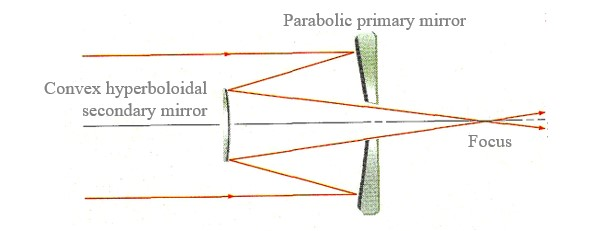
\includegraphics[width=9cm]{3.jpg}
        \label{}
    \end{figure}

L’idea è di sospendere uno specchio che prende il nome di “specchio secondario” (il nome è dovuto all’ordine con cui vengono colpiti dai raggi), che nel Cassegrain Telescope è un iperboloide, per poter estrarre il fascio sotto il primario. A questo punto il primario può anche essere forato (perché tanto è in ombra del secondario): questa è la configurazione con cui si costruiscono di fatto tutti i telescopi. I vantaggi di questa configurazione sono ovvi: l’oggetto più pesante, che è lo specchio, sta sotto, può avere montato lo strumento (lo strumento può essere grande quanto volete, anche molto più grande del telescopio stesso perché non impedisce alla radiazione di raggiungere il primario). Un vantaggio ulteriore di una configurazione di questo genere è che quando c’è un coma si manifesta elongato in una direzione sul primario ed elongato nella direzione opposta sul secondario, di conseguenza si compensano e questi sistemi permettono di avere una qualità ottica migliore. In più posso avere una lunga focale perché, se ricordiamo dall’ottica che la focale complessiva di un sistema ottico è 1/f = 1/f1 + 1/f2, posso avere focali molto estese in una configurazione meccanicamente molto compatta (a Serra La Nave vedrete un telescopio che ha una distanza tra il primario e il secondario che è dell’ordine di un paio di metri fisicamente, ma che ha una focale equivalente 1/f = 1/f1 + 1/f2 che è 16 metri), quindi posso avere una grandissima focale (che, ricordiamo, riduce le aberrazioni perché vanno con il cubo della focale) in una struttura estremamente compatta.

Una nota: potremmo pensare che mettendo un specchio proprio al centro di dove dovrebbe essere il soggetto non vedo il soggetto. Allora, ribadiamo il fatto che noi abbiamo un oggetto da osservare che è così lontano che lui, sorgente di onde sferiche, arriva come un fascio piano, (quindi è una direzione). Questo è il motivo per cui due persone riescono a vedere la stessa stella (per esempio, in un aula, mentre uno studente vede la porta, il prof. potrebbe non vederla perché messo in un punto in cui vede lo spigolo del muro e quindi c’è un problema di prospettiva: ciò perché la porta è vicina; se invece il prof. e lo studente guardano qualcosa di lontano, il fatto che loro siano posti in due posizioni differenti, non pone questo problema di prospettiva, perché non stanno vedendo porzioni diverse del fronte d’onda, ma la medesima). Quindi il fatto che lo specchio sia al centro, rompe il fronte d’onda, ne diminuisce il numero di fotoni, ma non la direzione e quindi l’immagine.

Quindi, per concludere, ribadiamo che il Cassegrain Telescope è fatto da un parabolico e da un iperbolico. 

Poi c’è un’altra configurazione, che è quella di Serra La Nave, che prende il nome di “Ritchey - Chrétien” dove sono due iperboloidi che compensano al meglio le aberrazioni tipiche delle ottiche (ricordatevi che le aberrazioni non sono solo difetti). 

\begin{figure}[h!!]
        \centering
        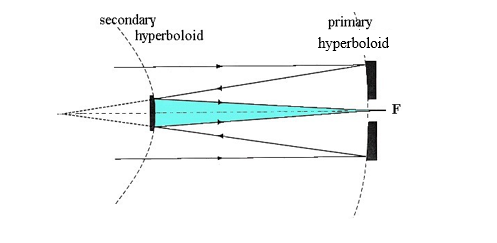
\includegraphics[width=9cm]{4.png}
        \label{}
    \end{figure}

Quindi, la maggior parte di tutti i telescopi è fatta, sostanzialmente, in questo modo.

Un po’ diversi sono invece i telescopi chiamati “gregoriani”. 

\begin{figure}[h!!]
        \centering
        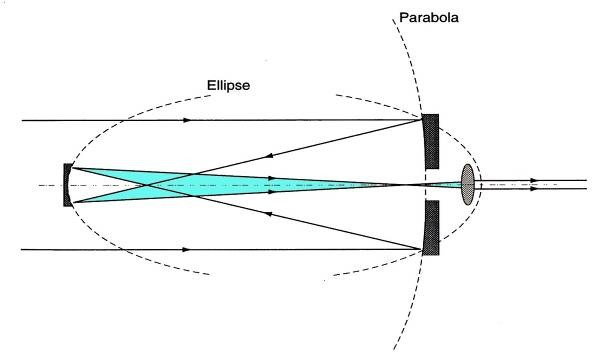
\includegraphics[width=9cm]{5.jpg}
        \label{}
    \end{figure}

Essi hanno il primario che è una parabola e il secondario che è una ellisse. Essendo coniche, perché siano allineate, devono avere il medesimo asse di simmetria e devono avere i fuochi coincidenti (se così non fosse, il sistema non sarebbe allineato, non avrà il fuoco). Il gregoriano è un telescopio tipico degli osservatori solari, perché il gregoriano ha un fuoco intermedio. Questo cosa vuol dire? Che io potrei, in linea di principio, collocare un disco (vedi immagine), per esempio, con un foro per vedere del Sole una piccola porzione. Potrei usare questo foro per ridurre la quantità di energia che dal Sole altrimenti arriverebbe sullo specchio (stiamo parlando di 1 kW/m2; se faccio un telescopio di 4 metri, mi ritrovo a dover dissipare una quantità di energia mostruosa, che posso dissipare tutta su questo diaframma dove faccio passare un pezzetto di luce del Sole che devo guardare). Quindi abbiamo questa configurazione che è tipica dei telescopi solari e anche di qualche radiotelescopio.\\

\subsection{Come è realizzato un telescopio}
Vediamo ora di cosa sono fatti i telescopi.

I telescopi sono fatti di vetro. Potremmo pensare di realizzare il telescopio di alluminio, di legno, ecc.: avrei ovviamente il problema di renderlo riflettente (infatti, se io costruisco uno specchio, lo specchio deve essere riflettente, basti pensare agli specchi di casa).

Quello che è riflettente è che dietro c’è uno strato di un metallo (solitamente è alluminio) che è depositato sul vetro e riflette la luce. Ora, nonostante il vetro sia un oggetto pesantissimo perché il vetro ha un coefficiente di espansione basso (stiamo parlando di uno 0,02 x 10-7 K) i telescopi sono fatti di vetro: ciò vuol dire che il telescopio mantiene la sua forma (ricordiamo che nella precedente sezione si parlava di micron di deformazione, che potrebbero essere dovuti a escursione termica). Il fatto che l’espansione termica sia di questo ordine di grandezza fa sì che una differenza di temperatura giorno-notte, inverno-estate (che può essere anche di 50° esagerando), è comunque tale da non cambiare la forma del telescopio. Questa cosa si fa praticamente con una fusione di vetro, come nella foto, dove una lastra di vetro di 8 metri, viene riempita di vetro, poi viene fuso, la vasca viene messa in rotazione e quando si raffredda si lavora per dargli la forma di iperboloidi, paraboloidi … Però, il fatto che è già in rotazione gli dà una forma che lo avvicina ad una parabola (notiamo che stiamo parlando, tra l’altro, di un oggetto che pesa 15 tonnellate).

\begin{figure}[h!!]
        \centering
        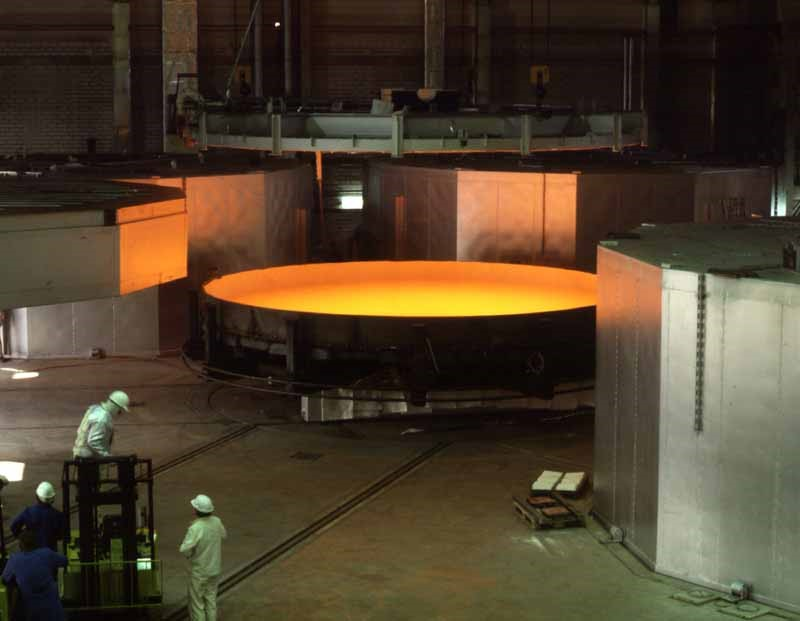
\includegraphics[width=7cm]{6.jpg}
        \label{}
    \end{figure}
    
Questo è tecnicamente il limite di quelli che sono i telescopi costruiti con un solo specchio, quindi detti “monolitici”. I telescopi più grandi vengono costruiti invece con un insieme di specchi sostanzialmente esagonali che vengono assemblati per dare la forma che si vuole (un po’ come il pallone da calcio, con gli esagoni puoi fare una sfera). Qui si vede il telescopio del Keck.

\begin{figure}[h!!]
        \centering
        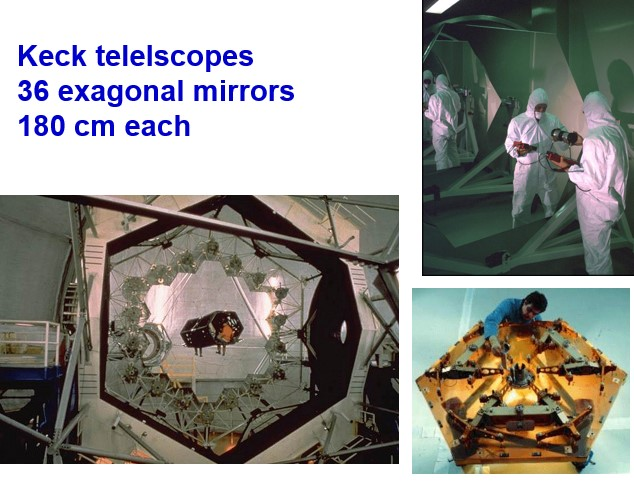
\includegraphics[width=7cm]{7.jpg}
        \label{}
    \end{figure}

Poco fa dicevamo che errori anche del micron rendono inutilizzabile un telescopio. Ma un oggetto così grosso e pesante come facciamo a lavorarlo? La lavorazione è un problema, l’allineamento è un altro problema. Infatti il monolitico non ha soltanto il compito di raccogliere la luce, ma ha anche il compito di spedire tutta la luce che arriva sul fuoco in fase, altrimenti non ha potere risolutivo (non è più una fenditura se le cose arrivano a caso). Quindi il problema principale di questo dispositivo è che gli specchi devono essere messi in maniera tale che la loro distanza sia esattamente un multiplo di ordini di lunghezza d'onda, altrimenti non andrà più in fase la radiazione. Se non sono in fase, quello che si otterrebbe è tanta luce, ma non si avrebbe potere risolutivo. Adesso vedremo come si risolvono questi problemi (il motivo per cui questi oggetti sono nati adesso è che adesso abbiamo una elettronica veloce, 20 anni fa non potevano funzionare o funzionavano male).

\subsection{Montature e proprietà del telescopio}
Allora, abbiamo visto come si fanno oggi i telescopi per cercare di ridurre le aberrazioni.  Facciamo finta che l’abbia fatto, ho preso due specchi e li ho messi uno sull’altro. Però adesso qual è il problema? Il problema è legato al fatto che devo osservare un oggetto che, nel mio sistema alto-azimutale, comunque sta sorgendo e tramontando. Per fare questo mi devo inventare una meccanica che possa permettermi di fare questa operazione. La prima meccanica in assoluto che è stata realizzata, è stata realizzata con questo obiettivo ed è stata la cosiddetta “montatura equatoriale”.

\begin{figure}[h!!]
        \centering
        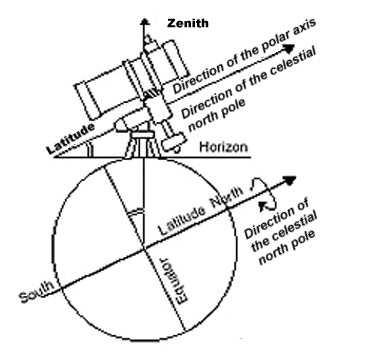
\includegraphics[width=7cm]{8.jpg}
        \label{}
    \end{figure}

Se io sedendomi voglio guardare il Sole, lo guardo, poi il Sole cresce e quindi un po’ mi giro, devo alzarmi e questo è un movimento complicato. Per ridurre questa complicanza, i telescopi sono stati montati su una montatura cosiddetta “equatoriale”. Si immagina di avere un proprio orizzonte, una verticale, che va verso lo zenit e un’asse che è parallelo all’asse di rotazione terrestre. Così facendo il telescopio deve solo ruotare attorno a quest’asse per compensare l’asse di rotazione terrestre, quindi deve girare esattamente all’opposto con la velocità dell’orologio (definizione). Questa è la montatura più diffusa ed è quella che abbiamo a Serra La Nave, e questo è un esempio di come si realizza (nella foto c’è uno dei telescopi di Serra La Nave quando era ancora in officina. Quindi abbiamo una sorta di forcella che ruota per tenere il telescopio sempre puntato sull’oggetto che, questa volta, descrive un cerchio nel sistema equatoriale).\\\\\\

\begin{figure}[h!!]
        \centering
        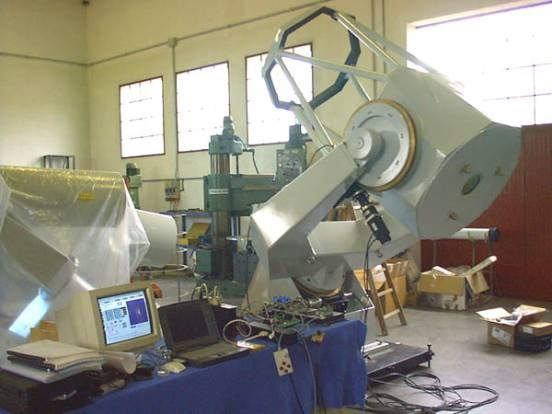
\includegraphics[width=9cm]{9.jpg}
        \label{}
    \end{figure}

Si tratta di un telescopio piccolissimo, perché questo  è un telescopio di 80 cm, però in realtà con questa montatura si facevano anche telescopi grandi. Nell’immagine seguente, per esempio, vi è la montatura “Fork mount” di un telescopio di 3,6 metri dell’ESO.

\begin{figure}[h!!]
        \centering
        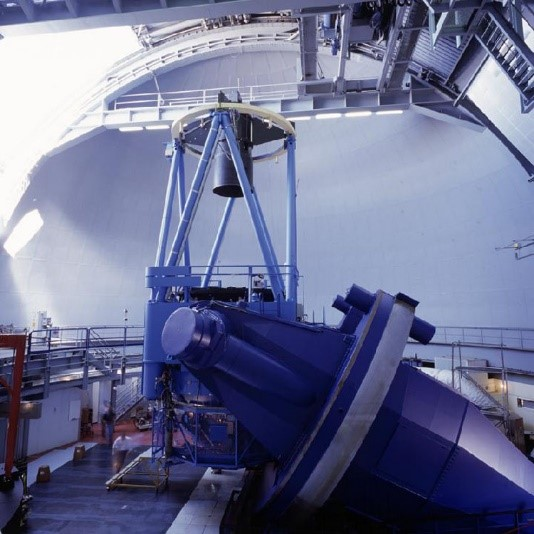
\includegraphics[width=9cm]{10.jpg}
        \label{}
    \end{figure}


Questa è stata, diciamo, la montatura storica di tutti i telescopi, fino a quando i telescopi non sono diventati troppo grandi perché, superate queste dimensioni dell’ordine di 4 metri, il telescopio diventa troppo pesante (vi dicevo prima uno specchio di 8 metri pesa 15 tonnellate, solo lo specchio; poi lo devo montare e questa roba diventa di molte decine di tonnellate). Questa montatura è stata abolita e sostituita da una montatura più semplice: la forchetta è stata messa dritta sul terreno. Sostanzialmente si è andati verso una montatura alto-azimutale, quella che dicevo prima, quella scomoda, che però ha un vantaggio: è meccanicamente facile da realizzare, sostiene il peso, non ci sono problemi. Con questa montatura alto-azimutale, per esempio, è stato realizzato il Telescopio Nazionale Galileo (TNG) (nella foto nell’officina e poi montato alle Canarie).

\begin{figure}[h!!]
        \centering
        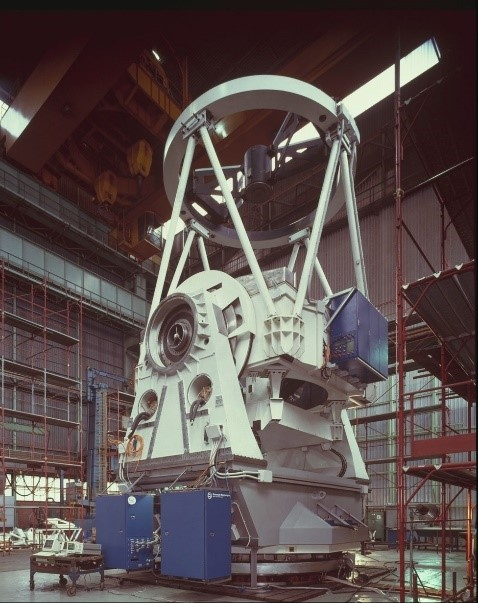
\includegraphics[width=5cm]{11.jpg}
        \label{}
    \end{figure}

Man mano che l’oggetto sorge, lui si gira verso est, sta quasi in orizzontale e poi, quando l’oggetto culmina, lui si porta a sud e si alza all’altezza massima dell'oggetto. Con questa montatura, si realizzano i più grandi telescopi: a questo punto la montatura è talmente grande che contiene tutti gli strumenti e non solo il telescopio, il cuscinetto in basso ruota, portandosi dietro il telescopio e tutti gli strumenti che sono montati insieme ai telescopi.\\\\


Risulta importante una proprietà del telescopio che lega il suo diametro alla sua focale, che si chiama “f-number”: sostanzialmente è un numero che esprime il rapporto focale/diametro (N=f/D). Questo perché? Perché quando i telescopi erano piccoli, uno poteva andare su f-number molto grandi, cioè focali lunghe, diametri piccoli. Man mano che i telescopi diventano più grandi, la focale non può più essere troppo grande rispetto al diametro, e allora queste focali diventano più corte, tanto corte che possono essere addirittura pari a 1 (perché se il telescopio è dell’ordine di decine di metri non puoi costruire un secondario che sta a 100 metri, devi comunque metterlo molto vicino).\\
Ammesso che abbiamo preso due specchi, li abbiamo messi assieme, li abbiamo messi su una montatura che è in grado di inseguire l’oggetto: il passo successivo è ovviamente guardare l’oggetto, avere un punto dove mettere noi, oppure gli strumenti. Quindi abbiamo bisogno di discutere di quali possono essere i fuochi di un telescopio. Abbiamo detto prima, per definizione, il fuoco dello specchio principale, o specchio primario, è il fuoco primario. In questa configurazione, ovviamente, non si possono collocare oggetti molto grandi e con gli anni gli strumenti sono diventati sempre più grandi. Per esempio nella foto l’Anglo Australian Telescope (AAT) ha un fuoco primario che ricomincia a diventare grande tanto quanto lo specchio primario e quindi non è utile. 

\begin{figure}[h!!]
        \centering
        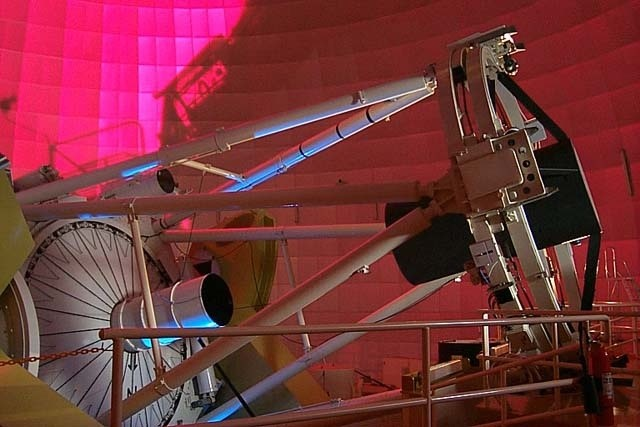
\includegraphics[width=5cm]{12.jpg}
        \label{}
    \end{figure}

Per questo motivo già Newton si era inventato la collocazione di uno specchio piano e estrarre il fascio focale per la posizione del sensore.

\begin{figure}[h!!]
        \centering
        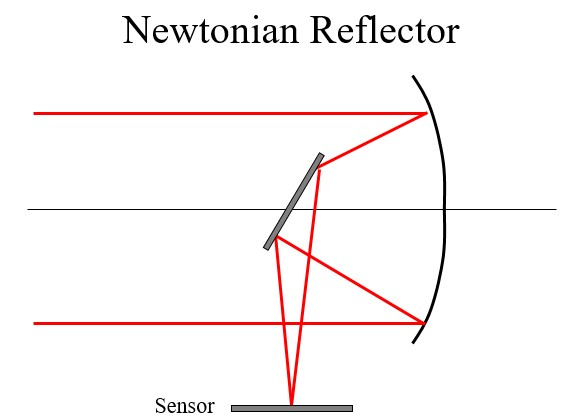
\includegraphics[width=7cm]{13.jpg}
        \label{}
    \end{figure}

Questo tipo di oggetto va bene per piccoli telescopi (cioè non si può immaginare un telescopio newtoniano di grandi dimensioni), \\
La configurazione che si è affermata nel tempo è la Cassegrain dove metti un secondario, che ti farà ombra (inevitabile), però ti permette di avere un fuoco fisso, dove tu puoi montare il tuo strumento. Questa cosa, però, ha ancora un problema: il tuo strumento lo devo montare al telescopio, il quale “andrà a spasso” seguendo gli oggetti con il mio strumento attaccato dietro (e questo è appunto grande e pesante, può essere pesante quanto un telescopio o forse anche più). Per esempio, a Serra La Nave c’è un telescopio di 1 metro di diametro e lo spettrografo è un banco ottico di 2,4 metri. Chiaramente non possiamo pensare di attaccarlo, dobbiamo trovare un modo per trasferire la radiazione dal telescopio allo strumento che non può stare attaccato; quindi si pone un problema: come faccio a mandare la luce in un posto considerato che invece il telescopio invece “se ne può andare a spasso”?

Esistono tante soluzioni: le prime sono state montature un po’ più complicate come quelle con il primario che riflette sul secondario, che riflette su un terziario ed estrae la luce. Quindi abbiamo una serie di specchi che rimandano la luce lungo l’asse di rotazione del telescopio. A questo punto, comunque il telescopio sia ruotato, qualunque cosa lui guardi, la luce arriva sempre nello stesso punto.\\ 
Queste montature permettono la realizzazione di grandi strumenti: sono strumenti che sono grandi quanto una grande stanza e vengono alimentati da uno specchio.\\
Una montatura molto utilizzata che permette l’estrazione del fascio è quella in foto: abbiamo il primario, il secondario e lo specchio (quello newtoniano). Stavolta lo specchio sta sotto il secondario, quindi non produce ombra e abbiamo il fuoco qui che viene chiamato “fuoco Nasmyth”, dal suo inventore.

\begin{figure}[h!!]
        \centering
        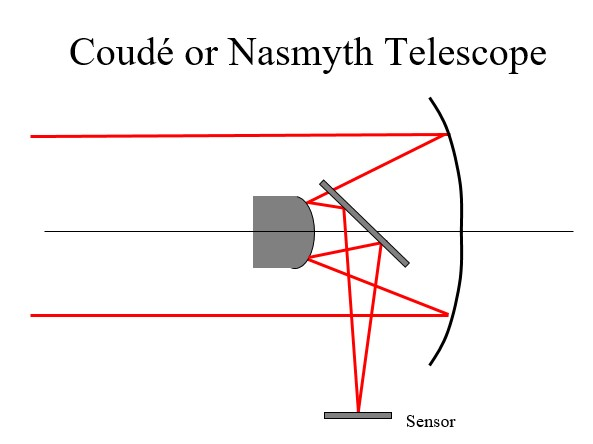
\includegraphics[width=7cm]{14.jpg}
        \label{}
    \end{figure}

Tutti i grandi telescopi attuali funzionano con questa configurazione. Si tratta, in definitiva, di telescopi alto-azimutali, primario, secondario, terziario Nasmyth e ovviamente ha due fuochi Nasmyth perché lo specchio sotto può essere girato.\\
Questa qui diciamo è la configurazione finale di telescopi attuali.

\subsection{Il processo di "coating"}
Abbiamo visto che il telescopio ha come primo obiettivo quello di raccattare tutti i fotoni che esistono e buttarli dentro il fuoco. È chiaro che l’efficienza non è soltanto una proprietà della dimensione dello specchio, ma dipende anche da quanto io sono bravo a rendere riflettente una superficie, che non è un concetto banale. Come si fa a rendere riflettente una superficie? Abbiamo detto prima che a casa abbiamo tutti un foglio di vetro nel bagno con dietro attaccato un foglio di alluminio: in realtà non è foglio di alluminio attaccato. Il processo si chiama “coating” o “deposizione”. Quello che succede è che si prende il vetro e nel caso dei telescopi si prende lo specchio di vetro e lo si deposita all’interno di una struttura come quella in foto che prende il nome di “campana”, che è un luogo dove si può creare il vuoto. 
\begin{figure}[h!!]
        \centering
        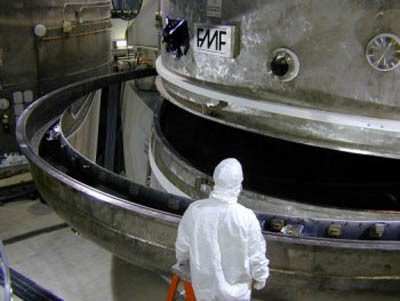
\includegraphics[width=7cm]{15.jpg}
        \label{}
    \end{figure}

Per cui io metto dentro il mio specchio, chiudo (è sigillato), con delle pompe tolgo tutta l’aria e dentro questa posso fare evaporare, per esempio, dell’alluminio. L’alluminio diventa un gas, riempie l’intera campana, quando si raffredda si deposita creando un coating, un deposito di alluminio sul vetro (ovviamente lo fa da tutte le parti, si deposita ovunque, si deposita sulla campana, ecc.). Ma perché questa procedura? Perché non lo vernicio? Perché se faccio questa operazione, io posso sapere esattamente qual è lo spessore di alluminio e so che l’alluminio si depositerà in maniera omogenea conservando la forma iniziale dello specchio (se io lo pennello ci saranno dei punti in cui c’è più alluminio, punti in cui c’è meno alluminio). Quindi questo permette di mantenere la forma.\\
\begin{figure}[h!!]
        \centering
        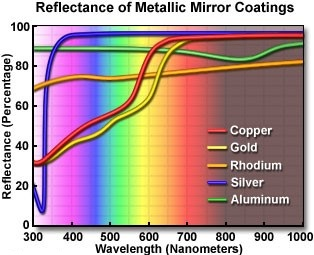
\includegraphics[width=7cm]{16.jpg}
        \label{}
    \end{figure}

Da un punto di vista quantitativo, osserviamo il grafico di seguito rappresentato: nella foto l’alluminio è la curva verde. Dal grafico si vede che non siamo in grado di produrre una riflettività del 100\%. Uno dei materiali più utilizzati è ovviamente l’alluminio perché è di basso costo; posso fare un deposito anche di oro, ma se lo facessi di oro scoprirei che la riflettività è una funzione della lunghezza d’onda e sarebbe molto alta nell’infrarosso e poco invece nella luce visibile (curva gialla). E allora, magari, l’alluminio è un buon compromesso per avere una buona riflettività su tutto, ma è una riflettività del 90\% (quindi 90\% sul primario, 90\% sul secondario fa l’80\% e già mi sono perso il 20\% di fotoni). Ogni volta che metto uno specchio mi perdo il 10\%). Quindi il coating d’argento oppure di oro è buono per l’infrarosso, per le lunghezze d’onda più grandi, cioè dove raggiunge il 95\% (l’alluminio ha un problema: dopo un po’ diventa opaco, quindi va tolto e rimesso; l’oro invece no).\\

 
\subsection{Uso degli attuatori}
Dunque per fare un telescopio bisogna prestare attenzione a dei fattori. Come si fa a far sì che funzioni nella realtà? Quando io costruisco un oggetto, questo si piega (ora magari non è tanto, perché è un oggetto rigido come uno specchio, però quel poco può essere un problema. Inoltre gli assi delle due coniche devono avere i fuochi coincidenti; se l’asse un po’ si sposta significa che non va più a fuoco). Quindi ho bisogno di una struttura che, non solo mi faccia girare il telescopio, ma mi garantisca anche qualità. Questa cosa non è facilmente ottenibile quando gli strumenti diventano grandi: la soluzione a questo nasce dall’idea che lo specchio in vetro, anche se è perfetto, non manterrà la sua forma (soprattutto a terra con la gravità). Allora, quello che si è immaginato è di costruire specchi non più tanto spessi come si faceva un tempo da sostenere la gravità da soli (a Serra La Nave, per esempio, abbiamo uno specchio di 1 metro che è alto 25 cm). Allora quello che si è immaginato è la seguente: costruisco uno specchio di vetro sottile (non grande, 20 cm, non di più), dopodiché lo poso su una struttura di metallo. In questa struttura di metallo, ci saranno degli attuatori (pistoni) che possono spingere o tirare, quindi quando il telescopio punta qualcosa, se si deforma, si tireranno gli attuatori giusti e si spingeranno gli altri perché il telescopio abbia la forma ottimale. Stiamo quindi parlando di ottica attiva e questo è l’unico modo per avere i telescopi effettivamente sempre ben allineati: anche in quello mosaico, in realtà, gli specchi non sono montati meccanicamente, sono montati su attuatori. In pratica si punta un oggetto, si fa un’analisi dell’immagine e vi si dà la forma perché l’immagine sia quella che è. È una cosa che si può fare facilmente perché esiste un’analisi del fronte d’onda (Polinomi di Zerniche), che ti dice come bisogna muovere gli attuatori perché lo specchio abbia la forma ideale. Così è costruito il TNG, ma oggi si va ad un passo successivo anche dove il secondario è attivo. Quindi, in pratica, io cambio queste cose fino a che non trovo la posizione ottimale degli specchi per avere le immagini al meglio.

\begin{figure}[h!!]
        \centering
        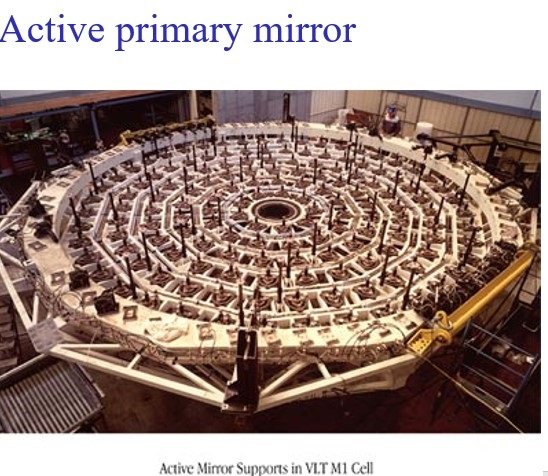
\includegraphics[width=5cm]{17.jpg}
        \label{}
    \end{figure}
    \begin{figure}[h!!]
        \centering
        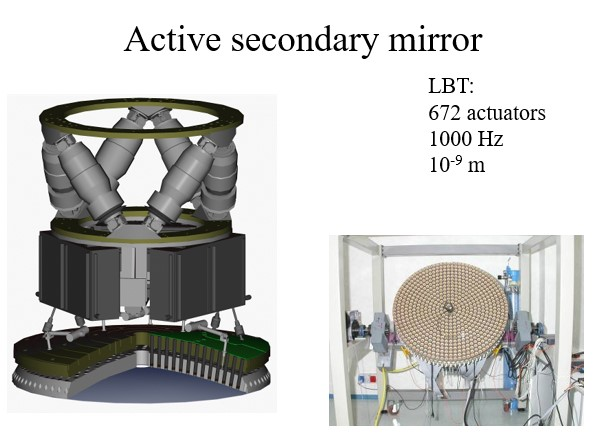
\includegraphics[width=5cm]{18.jpg}
        \label{}
    \end{figure}


\subsection{Il ruolo dell'atmosfera nell'osservazione, il "seeing" e l'ottica adattiva}
Immaginate adesso che dovete fare queste osservazioni di un oggetto che sta al di fuori dell’atmosfera terrestre. Cosa vuol dire? Vuol dire che la radiazione (che è effettivamente il fronte piano che arriva dalla stella) che a un certo punto impatta sull’atmosfera terrestre, prima di raggiungere il vostro telescopio avrà attraversato l’intera atmosfera e l'atmosfera produce una alterazione della radiazione. Ora, in maniera molto esagerata, è come quando voi guardate attraverso una atmosfera molto turbolenta e l’immagine dietro non è più chiara. Quindi quello che succede sostanzialmente è che l’idea che l’immagine di una sorgente puntiforme sia determinata dalla dimensione del telescopio potrebbe non essere più vera. Quindi, io ho un bel telescopio, l’ho costruito grande perché secondo me mi produce delle immagini di una certa qualità, ma scopro che questa cosa non è vera per colpa dell’atmosfera. In pratica succede che la radiazione incontra strati dell’atmosfera caratterizzati da un indice di rifrazione che ne produce lo spostamento spaziale: quindi arriva la luce della stella, arriva sul primo strato di atmosfera (facciamo finta che si possa immaginare fatta in strati) e qui l’indice di rifrazione non è 1, ma qualcosa di diverso e quindi cambia percorso, perché l’effetto è quello di avere una variazione della direzione; quindi si propaga, incontra un altro strato che avrà un altro indice di rifrazione e così via. Cosa accade? Accade che il risultato finale per me che osservo è che la stella sembra muoversi (e questo voi lo percepite anche quando guardate il cielo: i pianeti vi sembrano fissi, le stelle sembrano luccicare, perché in realtà quello che sta accadendo è che si sta muovendo). Ora, questa cosa qui si può vedere, ovviamente, come la matita nel bicchiere che si spezza. Ma si può anche vedere in un altro modo un po’ più sofisticato.

\begin{figure}[h!!]
        \centering
        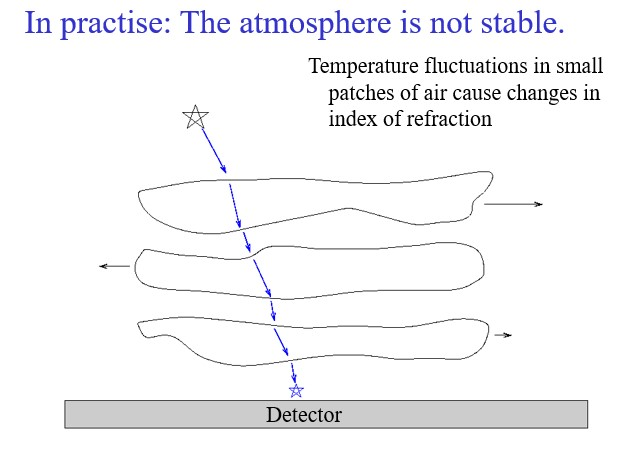
\includegraphics[width=9cm]{19.jpg}
        \label{}
    \end{figure}

Ribadendo ancora il concetto, l’atmosfera è in grado di aberrare l’immagine, per cui un’immagine, per esempio, perde i contorni. Il ruolo dell’atmosfera è quindi quello di vanificare la teoria di una sorgente le cui dimensioni siano assegnate solo dal diametro dello specchio perché la luce che viene giù dall’atmosfera incontra strati dall’indice di rifrazione diverso e comunque sempre diverso. Il risultato finale dell’osservatore è che la stella si muove sul piano focale. Quindi, io ho il mio telescopio, l’ho puntato bene, seguo la stella secondo i dettami della meccanica celeste, però la stella sembra che si muove. Il motivo di questa cosa qua è che in realtà il fronte d’onda piano che incontra l’atmosfera incontra celle dall’indice di rifrazione diverso (lo abbiamo visualizzato come se fosse tutto uno strato che cambia, però nella realtà, ogni porzione dell’atmosfera ha un proprio indice di rifrazione). Quindi, sul piano focale, in realtà, non si forma una sola immagine ma se ne formano tante, una per ogni colonna d’aria: ogni colonna d’aria mantiene la fase e il risultato è che sul fondo si formano tante immagini diverse che noi percepiamo come un allargamento dell’immagine, un perdere dei contorni dell’immagine. Questo accade per ogni colonna, dove ogni colonna cambia in continuazione le sue proprietà. Ora, naturalmente, quanto sia di qualità l’immagine dipende dal cielo: se guardate una stella al livello del mare vi appare in un modo. Man mano che si sale di quota, cioè si riduce la colonna d’aria, le cose vanno meglio ed è per questo che i telescopi si montano tutti quanti a 5000 metri quando è possibile. Questo effetto si chiama “seeing” ed è quello che in realtà dà la dimensione alle immagini delle stelle.\\
Una nota: la colonna d’aria in cui l’atmosfera è costante dipende dalla lunghezza d’onda. Quando parliamo di luce visibile si parla di 10 cm, mentre quando andiamo nell’infrarosso a 20 micron questa colonna d’aria è grande 8 metri, quindi gli effetti sono molto diversi sul telescopio. Se andiamo invece nel radio, la colonna d’aria in cui fronte d’onda non cambia è di 15 km quindi non ci sono tanti problemi.

\begin{figure}[h!!]
        \centering
        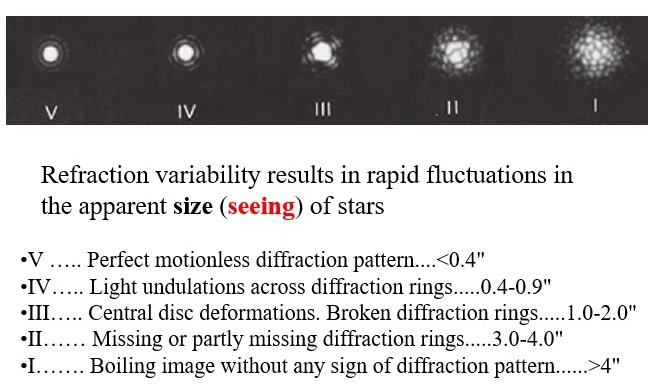
\includegraphics[width=9cm]{20.jpg}
        \label{}
    \end{figure}

Non sarebbe neanche un gran problema da un certo punto di vista perché, in fondo, non è cambiata la quantità di energia che è arrivata a terra (è sempre la stessa: l’ho sparpagliata). È un po’ più fastidioso se io considero il seeing per gli oggetti estesi. Ora, dicevamo prima che una stella sul livello del mare appare come 5 arcsec, mentre in un posto buono può essere 0,15; però, mentre questo è  per quanto riguarda gli oggetti puntiformi soltanto uno sbrodolamento dell’immagine su uno spazio più grande, è invece fastidioso quando si parla di oggetti estesi. Cioè, se voi provare a guardare con il vostro binocolo la Luna, allora sì che comincia ad essere un problema, perché si perde il contorno.\\ 
 Diamo ora la definizione di “seeing”: la lunghezza d’onda diviso il diametro della colonna d’aria dove le cose non cambiano.

  $$ \Delta\theta=\frac{\lambda}{r_0} $$

Il metodo con cui si risolve il problema delle deformazioni del fronte d’onda lungo l’atmosfera è che la radiazione deformata dall’atmosfera incide su uno specchio deformabile (posso dargli la forma che voglio, è uno specchio formato da un centinaio di attuatori, è molto sottile, sono dell’ordine di 1 mm e con tanti attuatori posso un po’ piegarlo). Quindi la luce che arriva dalla stella finisce su questo specchio adattivo e va verso il mio sensore, però prima lo intercetto con uno specchio che fa passare tutta la luce tranne un po’ (10\%), uno specchio detto “Beamsplitter” o semiriflettente. La parte riflessa la analizzo per scoprire come il fronte d’onda è stato deformato. Quindi dico allo specchio che forma deve assumere perché passi il fronte d’onda piano (è un loop, lui ogni centesimo di secondo fa l’analisi e cambia lo specchio, fa l’analisi e cambia lo specchio; 1 centesimo di secondo è il tempo con cui cambia l’atmosfera). Questa si chiamerà “ottica adattiva” (quella di prima era “attiva”).

\begin{figure}[h!!]
        \centering
        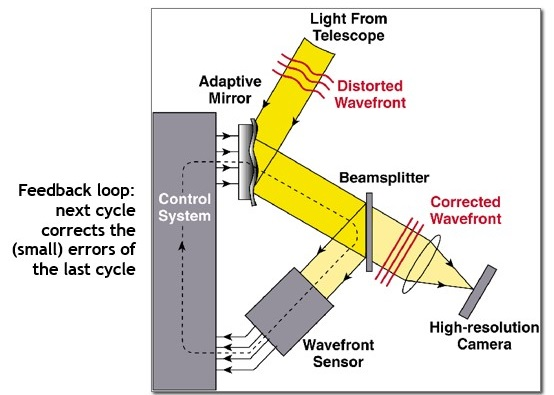
\includegraphics[width=11cm]{21.jpg}
        \label{}
    \end{figure}

\begin{figure}[h!!]
        \centering
        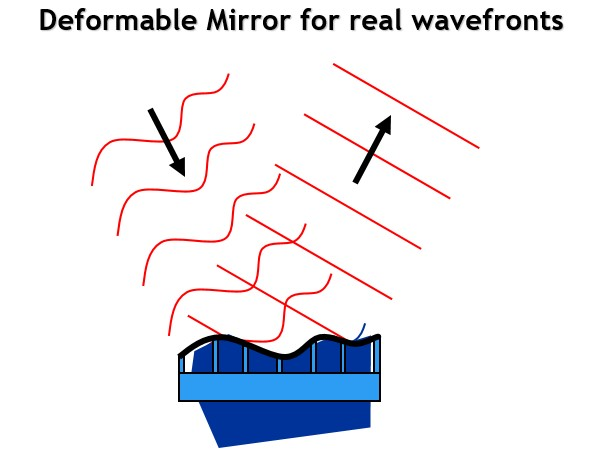
\includegraphics[width=9cm]{22.jpg}
        \label{}
    \end{figure}

Questo comunque è il sistema con cui un’immagine orrenda di una stella con un’analisi del fronte d’onda diventa quella rappresentata in foto.

\begin{figure}[h!!]
        \centering
        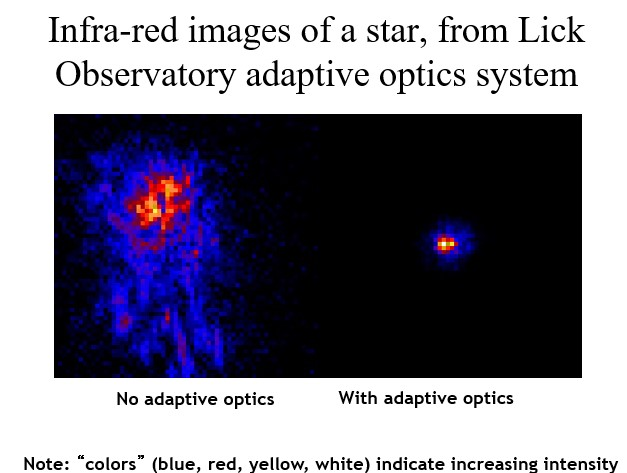
\includegraphics[width=9cm]{23.jpg}
        \label{}
    \end{figure}

\begin{figure}[h!!]
        \centering
        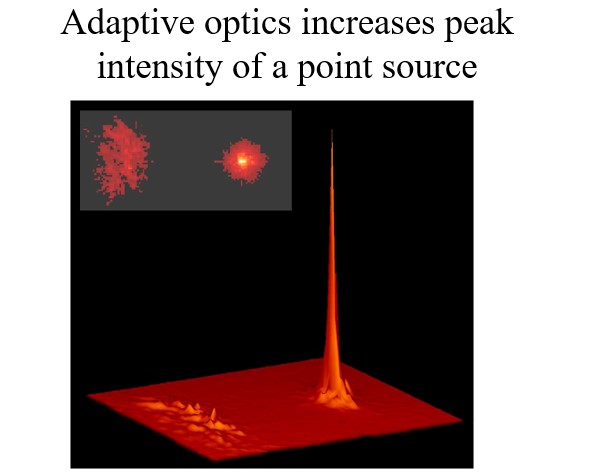
\includegraphics[width=9cm]{24.jpg}
        \label{}
    \end{figure}

Questo giochino qua si può fare quando posso tirare via un po’ di luce e fare l’analisi del fronte d’onda: ma l’analisi del fronte d’onda prevede che io abbia dei fotoni, quindi l’oggetto deve essere brillante (10). Se io sto studiando una stella più debole della decima, potrei usare una stella vicina (non devo fare l’analisi del fronte d’onda esattamente sulla stessa stella, ma dovrei guardare una che arriva magari da un altro angolo perché è una stella vicina in cielo, ma deve essere una stella brillante). A volte succede che non c’è: allora cosa si fa in questi casi? Basta avere associato al nostro telescopio un laser: sostanzialmente quello che si fa è quello di sparare con un laser nella direzione di osservazione. A 92 km dal mare in altezza abbiamo uno strato di sodio e il laser lo incontra. La frequenza del laser è esattamente la frequenza per creare una transizione atomica nel sodio (sappiamo che gli elettroni passano da un livello a un altro se colpiti da un fotone opportuno). Questo fotone, che è il nostro laser, con una lunghezza d’onda di 590 nm, trasferisce gli elettroni del sodio da un livello a un altro. L’elettrone non può però stare in uno stato eccitato, quindi decade e riemette un fotone. Ma il fotone, questa volta, viaggerà verso il telescopio e farà lo stesso percorso della luce della stella: quindi in pratica io costruisco una stella digitale vicino alla mia, di cui analizzo il fronte d’onda distorto e, anche se la mia stella è debole, non ha abbastanza fotoni, faccio quindi un’analisi di una stella che mi sono costruito da solo. Il sistema attuale più incredibile è uno che vuole la tua sorgente al centro e 4 stelle artificiali attorno per poter fare delle correzioni angolari (perché ci sono delle differenze): se io guardo in una direzione il fronte d’onda si deforma in un modo, se guardo in un’altra si deforma in un altro modo. Esiste un angolo magico in cui tutto è giusto e si chiama “isoplanatico”. Quindi si spara, si crea accanto alla nostra stella una stellina artificiale che è fatta di questo sodio che brilla, analizzo il fronte d’onda del sodio e mi faccio le mie correzioni sullo specchio deformabile.\\

Nota: esiste un tempo in cui le deformazioni sono uguali e questo si chiama “tempo di coerenza” (io ho detto che a spanne cambia ogni centesimo di secondo come ordine di grandezza). Quindi se tu analizzi il fronte d’onda in un millesimo di secondo, per il 99\% del tempo il tuo fronte d’onda sarà corretto e darà un’immagine giusta. Naturalmente, il tempo che ti serve per la tua analisi dipenderà da quanti fotoni hai. Con questo sistema tu lo puoi fare veramente in un millesimo di secondo (se la stella è debole, hai bisogno di più tempo). Quindi vuol dire che per più tempo l’immagine sarà più sbrodolata. Più è corto il tuo tempo di reazione più l’immagine diventa piccata. Quindi noi abbiamo un tempo, un angolo e uno spazio entro cui le correzioni sono giuste: questi sono i tre parametri. Questi parametri cambiano con la lunghezza d’onda; nel visibile sono molto brevi, nel radio diventano molto lunghi (quindi chi fa radioastronomia non ha in genere tanti problemi).\\
 
 \subsection{L'atmosfera come un prisma}
Allora, abbiamo visto quale è il problema di chi vuole fare osservazioni a causa dell’atmosfera: l’atmosfera rovina queste immagini, ma l’atmosfera si comporta come un prisma in quanto abbiamo detto ha un indice di rifrazione e, come tutti gli indici di rifrazione, dipende dalla lunghezza d’onda. Questa di seguito riportata è la formula che dice che l’indice di rifrazione cambia con la pressione e con la temperatura, quindi non si può prevedere: questo è il vero problema. 

\begin{figure}[h!!]
        \centering
        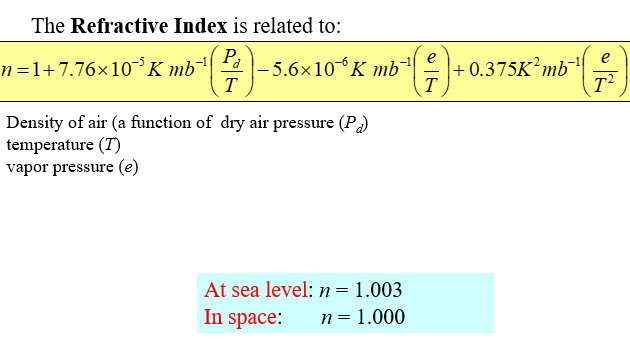
\includegraphics[width=9cm]{25.jpg}
        \label{}
    \end{figure}

Esiste un forte impegno da parte degli astrofisici per le previsioni: cioè noi studiamo le previsioni del tempo molto molto bene (all’ESO esiste un gruppo di lavoro il cui obiettivo è studiare l’atmosfera terrestre in modo da correggerlo, ma non è una cosa che si può fare. Per darvi l’idea di quello che succede, stiamo parlando di 3 millesimi di differenza tra ciò che sarebbe perfetto e ciò che invece non è perfetto).
\\Questo problema di rifrazione pone due effetti: la rifrazione è quella cosa per cui la radiazione cambia di percorso; quindi un problema della rifrazione è che le stelle non sono dove sembrano stare apparentemente. Questo pone un problema a chi punta un telescopio: dove lo dovrei puntare un telescopio? Verso la stella o verso la direzione apparente della stella che però dipende dall’indice di rifrazione che non è esattamente prevedibile (prevedibile su grande scala, ma non esattamente prevedibile)? Il puntamento esatto di una stella si può fare solo a posteriori (prima punti il telescopio, fai un’immagine, scopri dov’è e poi la posizioni sul sensore che poi devi utilizzare). Quindi le stelle non sono dove pensate siano: questo d’altra parte si vede anche con il Sole: quando il Sole tramonta, il Sole è in realtà molto più basso. 
\\Ma dicevamo che la cosa più fastidiosa dell’atmosfera è che questa si comporta come un prisma per cui si scompone la stella nei suoi colori. Sappiamo che la legge di Snell, nel caso perpendicolare alla superficie, non c’è spostamento dell’immagine, tutti i colori sono perfettamente sovrapposti; man mano che ci spostiamo in distanza zenitale si comincia a piegare in maniera diversa apparentemente con i colori, per cui abbiamo variazioni (quando l’oggetto è molto basso) che sono dell’ordine di 10 arcsec.
\\Questo significa che se tu fai una foto, la tua stella non è un cerchio, ma un cerchio allungato nella direzione verticale. Chi fa fotografie si è reso conto che le stelle allo zenit sono effettivamente tonde e quelle basse non sono tonde.

\begin{figure}[h!!]
        \centering
        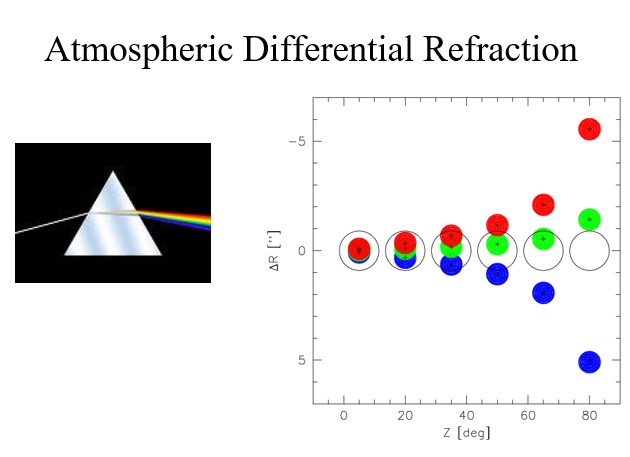
\includegraphics[width=9cm]{26.jpg}
        \label{}
    \end{figure}
\newpage
\subsection{Potere risolutivo di un telescopio}
Abbiamo parlato finora di telescopi, cioè di un oggetto che sostanzialmente è una fenditura circolare che raccoglie la radiazione, l’onda piana prodotta dagli oggetti, dando origine sul piano focale a una figura ben definita, a una Point Spread Function ben definita che si chiama tradizionalmente “disco di Airy”, dal signore che lo ha battezzato, che è una serie di anelli concentrici. Questo oggetto abbiamo detto ha una posizione, il primo zero, che è legato al diametro del foro di un telescopio.
\begin{figure}[h!!]
        \centering
        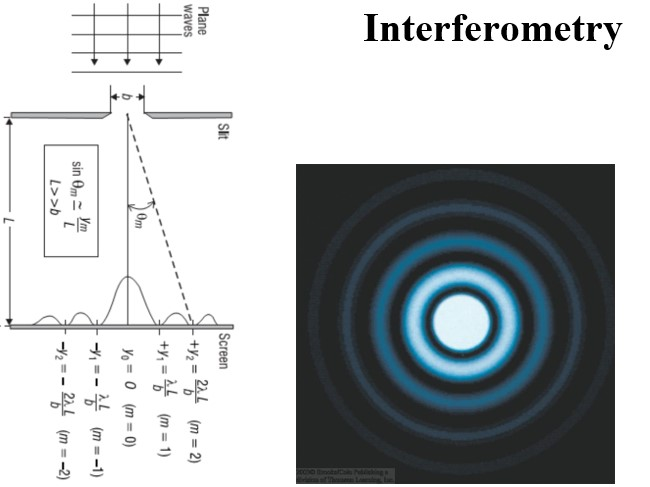
\includegraphics[width=9cm]{27.jpg}
        \label{}
    \end{figure}

\begin{figure}[h!!]
        \centering
        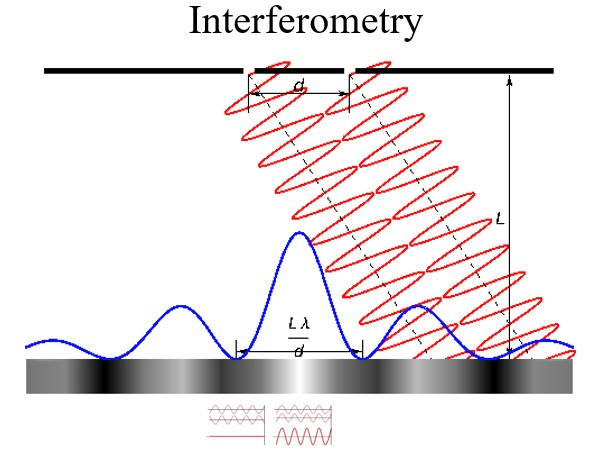
\includegraphics[width=9cm]{28.jpg}
        \label{}
    \end{figure}

\begin{figure}[h!!]
        \centering
        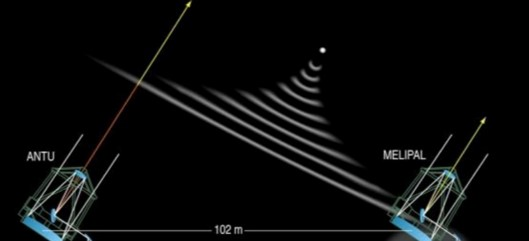
\includegraphics[width=9cm]{29.jpg}
        \label{}
    \end{figure}

Ora, esiste un modo di aumentare il potere risolutivo dei telescopi (perché di fatto questo limita la nostra capacità; un oggetto più piccolo del disco di Airy noi non lo possiamo vedere come risolto)? Allora, esiste la possibilità e si basa sull’interferometria: l’interferometria voi la conoscete benissimo ed è l’esperimento delle due fenditure. Adesso voi immaginate di non avere un solo telescopio, ma di avere due telescopi che guardano tutti e due nella medesima direzione la stessa stella. Quello che succederà, ovviamente, è che uno dei due telescopi vedrà il fascio di luce che arriva un po’ prima dell’altro, non saranno più in fase. Ma se uno attua una correzione della fase può effettivamente dare origine a una figura di interferenza. Se uno avesse due telescopi che guardano nel cielo la sorgente e correggesse quella differenza di cammino ottico potrebbe arrivare a fare effettivamente le frange di interferenza così come le fanno le due fenditure. Questa volta, però, lo zero non è più il diametro del telescopio, ma è la distanza delle due fenditure o la distanza dei telescopi che può essere, per esempio, dell’ordine di 100 metri, quindi avere un potere risolutivo che è 10 volte maggiore. 
\\Dov’è l’inghippo? L’inghippo è che la risoluzione angolare è solo la congiungente i due telescopi. Le frange, in una direzione, sono lunghe quanto sarebbe la risoluzione data da un singolo specchio, mentre lo sono separate nell’altra direzione quanto la distanza tra gli specchi. Se io prendo due specchi e li metto assieme posso creare una figura di interferenza lungo la congiungente dei due specchi; nell’altra direzione le due immagini rimarranno allungate esattamente come lo erano. 
\\Allora, cosa succede? Succede che potrei avere un elevato potere risolutivo angolare solo lungo la direzione dei due telescopi. Per poter fare qualcosa di meglio, dovrei avere più di 2 fori, di averne tanti ed è quello che si è fatto con uno strumento che si chiama Very Large Telescope Interferometer (VLTI) che prevede 4 telescopi di 8 metri più una batteria di telescopi piccoli.
\begin{figure}[h!!]
        \centering
        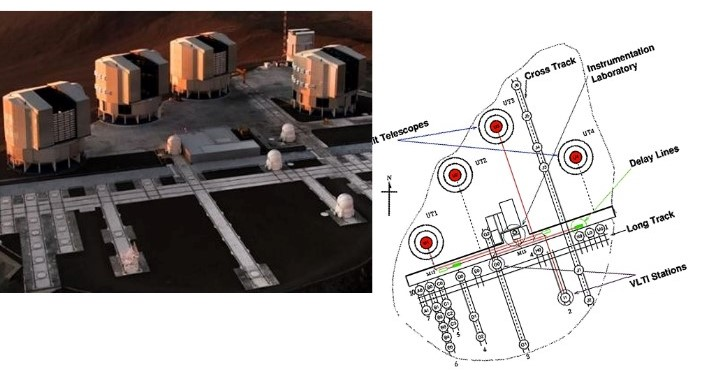
\includegraphics[width=9cm]{30.jpg}
        \label{}
    \end{figure}

Per ognuna di queste coppie si crea una figura di interferenza: cioè tutti i telescopi guardano il medesimo oggetto. A coppie di fenditure, a coppie di telescopi si crea una figura di interferenza. 
Cioè se io prendo i segnali di due telescopi e li interferisco, ma lo posso fare con tutte le coppie di telescopi creando una figura di interferenza dove ci sono distanze diverse (perché i telescopi hanno distanze diverse) e direzioni diverse. Il risultato di questa mega interferenza, di tutte queste figure che si sommano, può essere un’immagine che è effettivamente molto risolta in tutte le direzioni angolari.
\newpage
\subsection{Radio telescopi}
Abbiamo visto la parte ottica: noi possiamo osservare non solo con telescopi ottici, ma anche con telescopi radio (in foto il Telescopio di Noto). 

\begin{figure}[h!!]
        \centering
        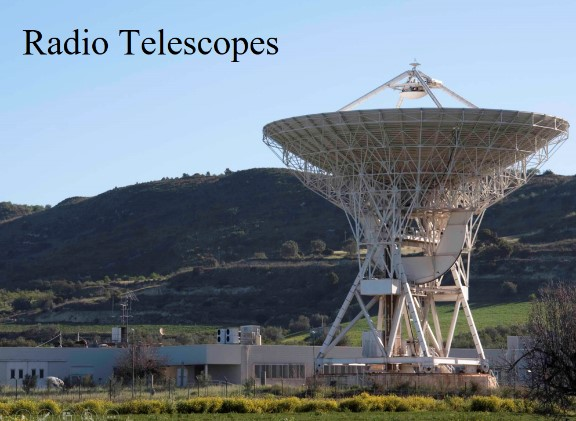
\includegraphics[width=7cm]{31.jpg}
        \label{}
    \end{figure}

I telescopi radio, rispetto a quelli ottici, non sono effettivamente diversi perché sono con montatura alto-azimutale e la larghezza di un telescopio non è molto diversa dalla focale. Il telescopio ha un fuoco primario su cui sono poggiati una serie strumenti (nel caso radio si parla di ricevitori, non si parla ovviamente di fotografie) e questi telescopi radio sono ovviamente molto simili a quelli ottici più grandi. Allo stato attuale, i telescopi radio più grandi al mondo sono “Green Bank” negli Stati Uniti con 43 metri e “Effelsberg” a Bonn di 100 metri, “Arecibo” di 300 metri che ha una caratteristica molto diversa: questo non si può orientare, lui osserva ciò che passa (il telescopio “Arecibo” è stato dismesso qualche anno fa ed è stato sostituito da questo telescopio cinese che si chiama “FAST” di 500 metri). 

\begin{figure}[h!!]
        \centering
        \includegraphics[width=7cm]{32.jpg}
        \label{}
    \end{figure}

I singoli telescopi in radioastronomia non hanno grande fortuna perché parliamo di lunghezze d’onda che sono decine di centimetri come grandezza e vale sempre, anche nel radiotelescopio, la famosa regola per cui la funzione di interferenza al primo fuoco vale $1,22*{\lambda}/d$, ma ${\lambda}$ vale centimetri questa volta. Nel radio l’interferometria è la tecnica maggiormente utilizzata.
Il radiotelescopio, però, così costruito diventa un interferometro con una base di 27 km. Allora diventa un potere risolutivo superiore a quello di quelli ottici. Il futuro degli interferometri si chiama “Square Kilometer Array (SKA)”: si parla di centinaia di telescopi che riempiranno l’Australia (costa ovest) e avranno una superficie di rapporto equivalente 1 kilometro. 

\begin{figure}[h!!]
        \centering
        \includegraphics[width=7cm]{33.jpg}
        \label{}
    \end{figure}

Il più famoso interferometro di cui avete sentito parlare adesso è quello che ha visualizzato il buco nero di M87 e il buco nero poi al centro della galassia. Questo è un array di telescopi che è distribuito su tutta la superficie della Terra. Sono state combinate le misure di varie antenne (una sta al Polo Sud, una in Danimarca, una vicino alle Hawaii, ecc.) Tutti questi hanno combinato i loro segnali per produrre un’immagine di quello che dovrebbe essere l’ambiente che circonda il buco nero; non è stata fatta la foto del buco nero, ma dell’ambiente che lo circonda. Queste misure sono fatte non nel centimetrico, bensì a 1,3 mm (230 GHz).

\begin{figure}[h!!]
        \centering
        \includegraphics[width=7cm]{34.jpg}
        \label{}
    \end{figure}

Nota: i telescopi prendono i dati a coppie. 
I radioastronomi, rispetto ai solari non hanno il problema del maltempo, perché le onde passano (la televisione la vedi anche se piove). La visibilità dell’oggetto può non essere simultanea per tutti i telescopi. L’Italia è al momento impegnata nella realizzazione del primo strumento dove il ricevitore è bidimensionale: cioè, finora il radio aveva una sola antenna e vedeva un posto solo; questo sarà un ricevitore bidimensionale e potrà fare un’immagine di tutto il cielo contemporaneamente. Bisogna solo decidere cosa vedere perché è troppa l’informazione che arriva.\\

Ma qual è il vantaggio del radio rispetto all’ottico? Le onde radio, rispetto all’ottico, hanno il vantaggio di non essere fermate dalla materia (cioè voi usate il telefonino anche dentro questa stanza, anche quando la luce non arriva, perché le onde radio attraversano le pareti in questo caso). Questo vuol dire che le onde radio sono in grado di propagarsi attraverso lo spazio, anche attraverso la materia dello spazio; noi possiamo vedere per esempio il centro della galassia che è invisibile all’ottico perché la luce, la radiazione visibile, che parte dal centro della galassia, viene fermata dalla materia che la circonda. Quindi il radio ha il vantaggio di farci vedere più lontano rispetto all’ottico.

\subsection{UV, infrarosso, X}

Allora, abbiamo visto il visibile, abbiamo visto il radio che, sostanzialmente, da un punto di vista strumentale è identico al visibile. Non possiamo vedere invece né l’ultravioletto, né l’X da Terra perché interviene l’assorbimento dell’atmosfera (vedi la curva di trasmissione nella figura).

\begin{figure}[h!!]
        \centering
        \includegraphics[width=7cm]{35.jpg}
        \label{}
    \end{figure}

Allora, per questa parte siamo costretti ad andare nello spazio, bisogna fare delle osservazioni spaziali. Però, mentre per i satelliti che vanno a guardare l’ultravioletto, così come alcune regioni dell’infrarosso, effettivamente non si vedono da Terra (se voglio guardare a questa lunghezza d’onda devo andare nello spazio) abbiamo comunque una tecnologia per l’ultravioletto e l’infrarosso identica a quella dei telescopi a terra.\\ 

Quello che invece fa un po’ di differenza sono i cosiddetti “Telescopi X”. Voi sapete che i raggi X hanno la particolare abitudine di attraversare la materia, quindi non è facile intercettarli. Allora come si fa in questo caso? L’idea è stata di utilizzare una riflessione radente. Quindi i telescopi X, che sono nello spazio, sostanzialmente sono fatti da una superficie curva che è una porzione di paraboloide, seguito da una superficie curva che è un iperboloide, per correggere e convogliare la radiazione sul sensore. Siccome non è possibile fare oggetti molto grandi, quello che si è utilizzato come tecnologia è stato quello di inserirli uno dentro l’altro in modo da aumentare la superficie di raccolta con una serie di telescopi concentrici uno all’interno dell’altro. È così che è stato realizzato il telescopio più famoso che è “Chandra” e che è in orbita . 

\begin{figure}[h!!]
        \centering
        \includegraphics[width=7cm]{36.jpg}
        \label{}
    \end{figure}

\begin{figure}[h!!]
        \centering
        \includegraphics[width=7cm]{37.jpg}
        \label{}
    \end{figure}

Per la tecnologia degli X nel 2002 è stato premiato con il Nobel il prof. Riccardo Giacconi.
\newpage
\subsection{I gamma}
Quindi rimane l’ultimo tassello, perché l’obiettivo è ovviamente quello di guardare ad un oggetto (gli oggetti emettono tutto, tu devi guardare tutte le radiazioni contemporaneamente). Abbiamo visto come sono fatti gli strumenti che arrivano dal radio fino agli X.\\ 
Rimane l’ultima parte, che sono i gamma, la parte più energetica dello spettro. È la parte tipica dell’alta energia.\\
Come si produce un fotone gamma? Il fotone gamma si produce sostanzialmente in due modi:\\\\
1) un modo è per Compton inverso (si ha un elettrone relativistico che colpisce un fotone normale (infrarosso normalmente) e gli cede la propria energia e quindi il fotone diventa altamente energetico.
Vediamo più nel dettaglio: esiste un fenomeno che si chiama Effetto Compton secondo cui un fotone può cedere la propria energia a una particella. Esiste anche la probabilità di avere il processo inverso, che si chiama Compton inverso: il Compton inverso prevede che un elettrone relativistico molto energetico, collida con un fotone e gli ceda al fotone la sua energia, cioè significa cambiarne la frequenza (la velocità è sempre c: c era e c deve rimanere, però la sua frequenza può crescere e passare dal visibile/infrarosso al gamma);\\\\ 
2) un’altra possibilità è invece di produrre gamma nelle reazioni nucleari (nelle prossime lezioni ne vedremo 2: una è la protone-protone e poi c’è il CNO in cui si trasforma idrogeno in elio, si fa un bel giro attraverso una serie di nuclei e in alcune di queste reazioni si producono gamma).\\\\

Ora questi gamma sono utili per studiare ambienti di alte energie. In Lab imparerete a identificare la presenza di energia di particelle. Normalmente i gamma venivano considerati particelle anche se poi in realtà sono dei fotoni, però succede che esiste un materiale noto come "scintillatore" che attraversato da un gamma produce fotoni (guardo con dei fotomoltiplicatori), però significa che io devo prendere questo oggetto, e lo devo mettere su un satellite da mandare in orbita. 

\begin{figure}[h!!]
        \centering
        \includegraphics[width=7cm]{38.jpg}
        \label{}
    \end{figure}

Questo lo abbiamo fatto. Esiste un satellite che si chiama “Fermi” che ha un rivelatore che si chiama GLAST (Gamma-ray Large Area Space Telescope) e questo produce la nostra informazione sui gamma visti come particelle che arrivano sul detector. Con questo, comunque, si è fatta la prima mappa dell’Universo in alta energia.\\
Ma i fotoni gamma, che non arrivano a terra, strano a dirsi, ma si possono vedere anche con i telescopi. Questo perché? A terra, cosa succede? Succede che una particella che arriva ad alte energie dall’atmosfera, produce una cascata di particelle (sciame). Allora quello che succede è questo: supponete che arrivi un gamma che produce uno sciame. Questo sciame è fatto di particelle che hanno una velocità superiore alla velocità della luce in aria, quindi producono radiazione di Cherenkov (lo scopritore dottorando è restato chiuso in una stanza molto buia per vedere l’emissione che particelle dalla velocità superiore alla velocità della luce nel mezzo producevano. Se tu hai una particella carica che si muove dentro un mezzo ad una velocità superiore alla velocità della luce, le molecole, gli atomi di questo ambiente vengono polarizzate al passaggio della carica elettrica. Quando poi ritornano alla configurazione iniziale, emettono un bagliore, che è stato appunto dedicato a Cherenkov e viene chiamato oggi luce Cherenkov). Quello che succede è che lo sciame che si propaga illumina il terreno con un cono di luce che è nel visibile (va da 400 a 800 nm). Lo stesso vale in acqua: in acqua è stata sfruttata la luce Cherenkov, cioè particelle veloci in acqua, per la detection dei neutrini del Sole per esempio. Allora, quello che succede, è che arriva un gamma, produce lo sciame, lo sciame fa questo flash che dura 5 ns su 10 fotoni al metro quadrato, noi mettiamo dentro un telescopio e guardiamo la luce che viene prodotta dal Cherenkov. In questo modo, se di telescopi ne mettiamo più di uno, riusciamo esattamente a capire da che direzione è arrivato il gamma. Questi Cherenkov Telescope sono telescopi normalmente creati con mosaici di specchi, sono di dimensioni molto grandi, non hanno una grande qualità ottica e di telescopi Cherenkov nel mondo ne esistono 4 array, perché da solo non basta, serve un insieme.
L’INAF ne ha due grandi alle Canarie, poi ne abbiamo uno negli Stati Uniti che si chiama Veritas, un array che sta in Namibia si chiama H.E.S.S. dedicato a Hess che ha scoperto i raggi cosmici e poi ne abbiamo uno in Australia (che non è molto efficiente) e quindi sostanzialmente possiamo fare una misura dell’emissione di raggi gamma usando anche telescopi tradizionali. 
Il primo telescopio Cherenkov è stato fatto nel 1985. Questi sono tutti progetti pilota nella realizzazione di un grande telescopio che si chiama “Cherenkov Telescope Array” in fase di realizzazione, si tratta di una attività distribuita su tutto il pianeta, tutti partecipano alla realizzazione del CTA che prevede centinaia di telescopi il cui prototipo si trova sull’Etna. In questo momento l’INAF sta realizzando un Path-finder di CTA, cioè uno strumento completo che anticipa quello grande (se si manifesta un problema non lo posso scoprire quando ho fatto 200 telescopi, lo devo scoprire, magari, quando ho fatto i primi 10. Quindi esiste questo Path-finder in fase di realizzazione a Tenerife che si chiama ASTRI).\\
Tutto questo perché, come dicevamo prima, una sorgente dobbiamo guardarla da gamma al radio (nella foto la sorgente è una galassia e la sua distribuzione in energia) 

\begin{figure}[h!!]
        \centering
        \includegraphics[width=7cm]{39.jpg}
        \label{}
    \end{figure}

Questo è il concetto moderno di astronomia in cui ognuno di noi deve essere in grado di comprendere i processi fisici che ci sono dietro ogni tipo di emissione: per esempio, per una Galassia bisogna chiedersi come è fatta per spiegare tutte le parti che vediamo).



\newpage
\section{Lezione del 17/10}
\subsection{Interazione radiazione-materia}
Tutto quello che accade nell’Universo lo possiamo sapere soltanto analizzando la radiazione EM, quindi dobbiamo cercare in essa la firma dei processi che l’hanno prodotta (la radiazione infatti viene emessa in modo diverso a seconda del processo).

La radiazione riflessa, per esempio, è polarizzata e possiamo sfruttare le proprietà della polarizzazione per studiare, per esempio, i processi che accompagnano una stella avvolta da un disco: infatti in tal caso la luce che arriva a noi è in parte riflessa dal disco e quindi polarizzata.
\newline
La luce può essere scatterata dalle particelle (es. polvere in aria). Nel caso dei gamma può avvenire il Compton inverso: la radiazione può cambiare la sua frequenza se interagisce con una particella che le cede la sua energia cinetica. 
\newline
Il Cherenkov \footnote{emissione di radiazione quando un mezzo è attraversato da una particella carica con velocità maggiore di quella della luce nello stesso mezzo} inverso è invece un processo che accade se e solo se la particella è relativistica: questa particella in genere è prodotta da reazioni nucleari, essa non può essere prodotta in altro modo.

Un altro esempio di emissione dovuta a particelle relativistiche è la radiazione di sincrotrone. Il sincrotrone è un acceleratore che grazie alla presenza di campi magnetici fa si che la traiettoria dell’elettrone sia circolare, ma quando una particella carica viene accelerata (in questo caso è una accelerazione centripeta) irraggia: la radiazione emessa da elettroni in moto su una traiettoria circolare si chiama radiazione di sincrotrone. Questa emissione avviene nel radio e porta la firma dell’elettrone e del campo magnetico che l’ha curvato.

Dall’analisi della radiazione possiamo capire quale evento l’ha generata: per esempio nel Sole si generano particelle cariche a velocità relativistiche che risentono del campo magnetico solare emettendo radiazione di sincrotrone; non vediamo la particella, ma dalla luce di sincrotrone ricostruiamo l’ambiente che l’ha prodotta. Ovviamente non è detto che il problema abbia un’unica soluzione, nel senso che si potrebbero avere altre condizioni che generano la stessa radiazione: bisogna allora cercare conferma in altri fenomeni.
Consideriamo infatti l’urto tra due atomi di idrogeno: durante la collisione viene trasferita energia, l’elettrone passa al livello più alto e poi decade emettendo un fotone di lunghezza d’onda caratteristica del salto energetico nel s.d.r. dell’atomo che emette. Se l’atomo si muove la lunghezza d’onda misurata da un osservatore fermo è diversa per effetto Doppler, la differenza mi da informazioni sulla velocità dell’atomo che emette. In questo modo abbiamo una conferma che si tratta di Cherenkov inverso.
%Se ho una massa di atomi di idrogeno che viene attraversata da un protone a velocità relativistiche; può succedere che uno di questi protoni rubi un elettrone a un atomo e lo colloca a un livello alto, questo decade con una velocità che non è quella ordinaria, ma è molto grande: questa è la conferma che esistono protoni ad altissima energia e quindi il Cherenkov inverso è vero.
Bisogna usare tutto ciò che conosciamo sulla interazione radiazione-materia per estrarre informazioni sulle sorgenti.

\vspace{3mm}
\subsection{Acquisizione dati in astrofisica}
 Supponiamo di voler studiare oggetti nel cielo analizzando la radiazione: nella pratica significa che a un certo istante di tempo guardiamo in una direzione e riceviamo una intensità specifica (una misura dell’energia normalizzata da tutto ciò che potrebbe alterarla), questa cambia con la posizione, con il tempo e con la frequenza. 
\newline
E’ importante conoscere lo strumento con cui sono state effettuate le misure. Immaginiamo di avere un detector bidimensionale fatto di quadratini che si accendono quando vengono colpiti dalla luce ovunque arrivi il fotone: se arriva un cerchio comunque noi vediamo accendere un quadrato. Quindi dagli strumenti dipende ciò che crediamo di aver visto.
\newline
Anche la cadenza con cui si fanno le osservazioni ci può dare un risultato sbagliato. Immaginiamo per esempio una persona che tutte le sere a mezzanotte misura la luce di una stella registrando sempre lo stesso numero di fotoni; egli si convince che l’intensità è costante, poi fa una misura a notte fonda e si accorge che il risultato è diverso: ciò vuol dire che il fenomeno ha una periodicità che è inferiore a un giorno.
\newline
 L’importante quando si costruiscono gli strumenti è che essi ci permettano di capire quali sono i limiti della misura, non si può pensare di analizzare un dato per verificare una teoria senza sapere come il dato è stato acquisito.
\newline
Ci chiediamo come si fa a ottenere un’immagine del cielo sapendo che questa dipende dalla lunghezza d’onda. Gli strumenti infatti danno tutti una risposta di tipo si/no (si accendono o non si accendono), essi ci permettono di misurare l'intensità, ma non il colore. Allora ci chiediamo come fa la macchina fotografica a fare le foto a colori: questa è fatta da tanti dispositivi, davanti ai quali ci sono dei filtri colorati rosso, giallo e blu; si fa la conta dei fotoni dei tre colori e in base a ciò si produce la foto a colori, ma non sono esattamente gli stessi colori che vediamo. 
\newline
Dobbiamo acquisire dati non solo spazialmente, ma anche in lunghezza d’onda. Abbiamo visto che la capacità di risolvere due stelle dipende dal diametro del telescopio in base al criterio di Rayleigh, quindi dobbiamo raccogliere la luce con un grande telescopio, poi questa immagine (disco di Airy) la dobbiamo mettere dentro un detector(sensore). Ricordiamo che una stella di magnitudine $0$ emette $1000 fotoni/(cm^2 \cdot s \cdot 
\text{Å})$.

\vspace{3mm}
Il detector lo abbiamo descritto come un oggetto che raccoglie fotoni, ma questo deve avere alcune caratteristiche: idealmente dovrebbe raccogliere fotoni di tutte le lunghezze d’onda (nella realtà non è possibile), inoltre per ogni fotone che arriva deve stabilire l’istante in cui è arrivato e la direzione da cui è arrivato, deve essere in grado di distinguere due fotoni che arrivano quasi contemporaneamente, deve avere un lungo tempo di integrazione e un numero grande di pixel (per distinguere esattamente la direzione dei fotoni), inoltre lo strumento deve essere in grado di misurare il grado di polarizzazione perché questo ci da’ informazioni sulla sorgente . Nella realtà non esiste un tale detector ideale, anche se esistesse avremmo comunque un problema di archiviazione dei dati.
\newline
Spesso inoltre gli eventi non sono correlati in maniera lineare (non è che se arrivano due fotoni c’è il doppio di corrente) perché a un certo punto c’è una saturazione: l’aumento eccessivo di luce non produce un ulteriore aumento del segnale.
\newline
 Ci sono tanti parametri che caratterizzano un detector, i più importanti sono due:
 \begin{enumerate}
     \item la sensibilità, o quantum efficiency, che è il rapporto tra il numero d fotoni riconosciuti come eventi diviso quelli incidenti (in genere l’efficienza quantica della CCD di un telescopio è dell’ordine del 95\%, quella della fotocamera di un cellulare è del 30\%);
      \begin{figure}[h!!]
        \centering
        \includegraphics[width=9cm]{astro1.png}
        \label{}
    \end{figure}
     \item il range dinamico, che è la quantità di segnale che può essere registrata: c’è un valore minimo e un massimo, che può dipendere da aspetti hardware o numerici (display a 3 cifre).
 \end{enumerate}
\vspace{3mm}
In passato si usava come detector la lastra fotografica, basata sul fatto che lo ioduro di argento può essere sospeso su una gelatina e quando viene colpito da un fotone produce qualcosa di annerito. La lastra fotografica ha rivoluzionato l’astrofisica perché permette di vedere anche lunghezze d’onda maggiori di quelle che vediamo con i nostri occhi: essa riportava dunque stelle non visibili altrimenti. Il grande svantaggio è che questo strumento è analogico: i dati non possono essere digitalizzati e archiviati.
 Poi sono arrivati i fotomoltiplicatori: all’arrivo di un fotone lo strumento rilascia un elettrone, che viene accelerato da una ddp, impatta su una lastra di metallo (dinodo) liberando un numero maggiore di elettroni, che poi vengono accelerati in cascata da una corrente leggibile.
 \begin{figure}[h!!]
        \centering
        \includegraphics[width=10cm]{astro2.png}
        \label{}
    \end{figure}
 \newline
Oggi si utilizzano i CCD, che sono oggetti tridimensionali, costituiti da una matrice di sensori tutti uguali, con pixel da 4 a 24 micron (quelli usati in astrofisica sono più grandi di quelli presenti nei nostri cellulari). Questi si basano sull’effetto fotoelettrico: arriva un fotone e se ha energia sufficiente libera un elettrone; ovviamente c’è un problema di soglia, nel senso che i fotoni con energia inferiore al lavoro di estrazione non sono rivelabili. 
\newline
\begin{figure}[h!!]
        \centering
        \includegraphics[width=6cm]{astro3.png}
        \quad \includegraphics[width=9cm]{astro4.png}
        \label{}
    \end{figure}
\newline
\newpage
Quando arriva il fotone, un elettrone passa dalla banda di valenza a quella di conduzione; si collocano sopra 3 elettrodi, quello al centro è positivo e i due lateralmente negativi, quindi l’elettrone resta intrappolato. Più fotoni arrivano più elettroni vengono intrappolati, alla fine gli elettroni vengono spostati verso un lettore di corrente cambiando la polarità degli elettrodi (da $-+-$ a $-++$). C’è chiaramente un tempo di lettura non trascurabile. 
\newline
Il CCD ha il grande vantaggio di avere una immagine digitalizzata e di darci informazioni sulle coordinate grazie ai pixels. Abbiamo detto che la risposta di una lastra fotografica non è lineare: questa si attiva solo quando è colpita da un certo numero di fotoni, poi la risposta cresce, ma va a saturazione. I CCD invece hanno una risposta lineare. Questi strumenti hanno permesso di migliorare l’efficienza dei telescopi: un telescopio equipaggiato con un CCD può essere più piccolo di un fattore 100 di un telescopio con lastra fotografica e l’efficienza sarà la stessa (ma la risoluzione peggiora).
\newline
\begin{figure}[h!!]
        \centering
        \includegraphics[width=9cm]{astro5.png}
        \label{}
    \end{figure}
\newline
\subsection{Imaging}
 I CCD sono stati inventati negli anni ‘60 come storage dei computer, ma poi si è capito che si potevano usare come dispositivi fotografici. Vediamo come si fa a trasformare una informazione continua in una immagine pixelata: sappiamo che ogni segnale si può esprimere mediante trasformata di Fourier, ma nella rappresentazione in armoniche c’è un taglio in frequenza sopra e sotto: non potrò mai registrare una lunghezza d’onda maggiore della dimensione del sensore, ma anche le lunghezze d’onda troppo piccole tanto da ricadere tutte all’interno di un pixel si perdono.
 \newline
\begin{figure}[h!!]
        \centering
        \includegraphics[width=9cm]{astro6.png}
        \label{}
    \end{figure}
\newline
Quindi l’immagine ci appare diversa da come è nella realtà proprio perché si perdono alcune frequenze. Inoltre quando i fotoni presenti in un pixel vengono letti come corrente facciamo una scelta: con quanti bit rappresentare il segnale. Ciò è importante perché il CCD non può contenere troppi elettroni oppure ci può essere una perdita nel processo di archiviazione: alcune informazioni si conservano nell’archiviazione e altre si perdono e ciò determina la risoluzione dell'immagine, ma più informazioni archiviamo più tempo ci vuole. Un’altra grossa limitazione è il numero di pixel: più ne ho, più spazio occupo, più tempo serve per trasferire i dati. In base a cosa vogliamo vedere scegliamo le caratteristiche ottimali del CCD. 
\newline
Inoltre il funzionamento è influenzato dalla temperatura: se si raffredda il CCD allora il numero di elettroni che passano spontaneamente in banda di conduzione è trascurabile, quindi si riducono i rumori. Un vantaggio importante dei CCD è che sono riutilizzabili; inoltre essi sono piccoli, ma si possono mettere più unità in un mosaico.

\newpage
\section{Lezione 21/10}
\subsection{ASTRONOMICAL TECHNIQUES: PHOTOMETRY}
Nella lezione di oggi vediamo cosa effettivamente riusciamo a fare misurando la quantità di energia che arriva da una stella. In linea di principio delle tante stelle viste sono state già fatte tante fotografie. Che cosa di quantitativo si può ottenere da queste immagini. Se ricordate, abbiamo definito la magnitudine come -2.5 log delflusso; che è l’energia [3.42], quindi in qualche modo abbiamo qui delle informazioni quantitative, che abbiamo inteso come numeri. In questa definizione la differenza di magnitudini tra due stelle è il rapporto dei flussi, quindi, la possibilità di comparare una rispetto ad un'altra in termini di percentuali. In questa scala viene definita come una differenza – come detto in qualche lezione precedente.
\newline
La fotometria nasce come magnitudine visuale: ciò che noi possiamo vedere ed in quest’epoca si poteva classificare gli oggetti più brillanti ed evidenziare la posizione nel cielo; quindi, abbiamo visto una sorta di astronomia di posizione. La fotometria – come la intendiamo oggi – nasce a metà dell’Ottocento, quando un Bond ha la magnifica idea di mettere al fuoco del telescopio una macchina fotografica: in questo momento comincia l’utilizzo della fotometria in termini quantitativi. La prima e grande scoperta di Bond nel fare fotografia fu che la dimensione dell’immagine di una stella su un piano focale (lastra fotografica a quell’epoca, oggi CCD [5:42]) è tanto più grande quanto maggiore è la luminosità dell’oggetto. Si passa quindi da una misura soggettiva sulla brillantezza ad una misura oggettiva, dove misuro il diametro dell’immagine della stella. Questo è stato il punto nodale di tutto: si potevano fare delle misure veritiere per tutti ed erano ripetibili, secondo i principi della fisica ecc..
\newline
L’ulteriore scoperta di Bond fu che quando osservava la lastra (impressionata dalle stelle) osservava stelle sulla lastra che non riusciva a vedere ad occhio nudo, questo pose un grande problema: come era possibile che il cielo sulla lastra fotografica è diverso da quello che vediamo con gli occhi? Per capire questa cosa – discorso fatto dal prof come evoluzione temporale: si era visto alla serra la nave in cui si riportava l’efficienza quantica sui ccd [7:35- rispiegazione 8]. Quindi il motivo per cui Bond vedeva sulla lastra fotografica oggetti che non vedeva con gli occhi è che la lastra fotografica ha un’efficienza quantica, non tanto più alta, ma quanto molto più estesa in lunghezza d’onda rispetto alla porzione del visibile dell’occhio umano; quindi, la lastra fotografica registra fotoni per es. da 300 nm che l’occhio umano non vede. A questo punto si definisce  una magnitudine fotografica, ossia una luminosità degli oggetti diversa dalla magnitudine visuale. Il motivo di tale differenza sta nella differenza che la lastra fotografica riesce a registrare tutta la lunghezza d’onda, poiché effettivamente non tutti gli oggetti emettono allo stesso modo – ci sono oggetti che emettono più a lunghezze d’onda lunghe e altri oggetti che emettono a lunghezze d’onda più brevi; quello che chiamiamo ultravioletto oppure infrarosso – in questa foto della galassia possiamo vedere che il cielo sta emettono principalmente in infrarosso, poi si passa alla luce visibile in cui si vede questo disco ed infine si passa agli oggetti più esterni che emettono soltanto nella luce ultravioletta; quindi, in conclusione, vedere in maniera diversa in realtà significa vedere corpi con proprietà emissive diverse. Quindi se noi riusciamo ad associare un flusso alle lunghezze d’onda che cosa possiamo misurare? Per dirlo facciamo un po' di ripasso e ricordiamo concetti noti.
\newline
\subsection{Conoscenze note}
PREREQUISITI: La radiazione apparentemente bianca in realtà è una sovrapposizione spaziale di radiazione di diversa lunghezza d’onda, che si possono separare con uno strumento chiamato spettrografo e che può essere rappresentato con un triangolo di vetro; sapete che l’indice di rifrazione dipende dalla lunghezza d’onda e quindi si piegano i fasci in modo diverso e da questa parte anziché vedere la stella vedrò la stella nei suoi diversi colori. Questo primo esperimento fu fatto agli inizi del 1800 con la luce del Sole da Fraunhofer che ottenne lo spettro del sole e si accorse che aveva una diversa luminosità con i colori, ma in più si rese conto che lo spettro era attraversato da bande in assorbimento, da strisce buie. F. le catalogò con delle lettere dell’alfabeto. Cosa stesse vedendo fu un mistero per più di 50 anni, quando finalmente due chimici tedeschi [nomi 12:20] in laboratorio furono i primi a divertirsi a fare spettri di fiamme: avevano un fornelletto in cui bruciavano i sali. Si accorsero che lo spettro di queste fiamme era sostanzialmente nero con la lunghezza d’onda, ma solcato da linee luminose, che cadevano in regioni diverse e quindi si vedevano con colori diversi. L’esperimento successivo che si sono inventati è stato quello interporre al Becco di Bunsen che bruciava sostanze una sorgente continua e scoprirono che la sorgente continua, come si aspettavano in origine, non desse origine ad un arcobaleno, ma questa volta quelle che prime erano emissioni di luce qui apparivano come bande e quindi era un assorbimento. Mancava la luce laddove invece qui risultava presente. Questi esperimenti sono stati di fatto la nascita dell’astrofisica, cioè l’idea di poter applicare le leggi della fisica per la convenzione degli astri. 
\newline
\subsection{Applicazione nello spettro solare}
Allora nel Sole abbiamo a che fare con una distribuzione di luminosità e questo oggetto continuo noi lo chiamiamo spettro che sarebbe la quantità di energia per lunghezze d’onda. Abbiamo nel Sole due caratteristiche: una distribuzione continua della luce e delle bande in assorbimento. Cerchiamo di associare a queste due proprietà un’origine che risale all’Ottocento e ci si rese conto che la distribuzione di luce e quindi lo spettro quindi la distribuzione dei fotoni con la lunghezza d’onda dei corpi cambiava con la lunghezza d’onda. C’era sempre Kirchhoff che si divertiva a registrare lo spettro di corpi con temperature diversa; ovviamente Kirchhoff non fece questo, ma il risultato era che se un corpo caldo produceva uno spettro con una forma caratteristica, il cui massimo che presentava andava sempre a lunghezze d’onda più brevi man mano che la temperatura del corpo aumentava. Vedi MQ questo andamento caratteristico è descritto matematicamente dalla Planckiana; la distribuzione di Planck dice che tutto dipende da un’unico parametro: la Temperatura; tutto il resto sono costanti: velocità della luce, costante di Planck, costante di Boltzmann che si utilizza per convertire i gradi in energia. Quest’andamento non è dei corpi caldi, intesi come oggetti che posso mettere su una fiamma e far bruciare; è in realtà dei corpi caldi, dove si raggiunge una condizione di equilibrio; si può riprodurre in maniera ragionevole in laboratorio contenendola la materia all’interno di una sfera per cui la radiazione va in equilibrio con la sfera stella e se noi pratichiamo un piccolo foro possiamo vedere questo tipo di emissione. Questo giochino lo fece Kirchhoff nel 1860 aveva una “lavatrice” guardava dall’oblo e riscaldava. Alle temperature come queste, fondava tutto, già si rese conto di questo andamento.  Allora nasce la possibilità di associare, grazie al fatto che la distribuzione sia una planckiana per un corpo nero, la posizione del massimo alla temperatura:  in questo grafico ][] vedete che il massimo di un corpo con la temperatura  6000K cada esattamente tra il verde e il giallo dove cade lo spettro del Sole. Quindi allora è possibile spontaneamente dire che il Sole è in superficie, almeno, una sfera con la temperatura di 6000 K ed il resto lo sia potuto vedere con T più basse. Quindi nella distribuzione continua di un corpo possiamo estrarre la temperatura con la Legge di Wien. Se si fa l’integrale di questa planckiana si ha una quantità che cresce con la temperatura alla quarta. Questo succede a terra, noi che cerchiamo di associare questo argomento agli astri… non possiamo partire dal principio che la stella sia una planckiana , perché non lo sappiamo ancora, quello che sappiamo è che il Sole, per esempio, ha una distribuzione di spettro continuo e ci sarò una magnitudine Bolometrica, cioè l’energia totale facendo l’integrale, poi successivamente ipotizzare che il Sole sia un corpo nero e quindi posso associare una temperatura del sole, quindi misurando l’energia che arriva e la divido per la costante di Stefan-Boltzmann. Allora posso assegnare al Sole una temperatura semplicemente misurando l’energia totale e dividendola per la costante di Stefan Boltzmann.
\newline
Ora non pensate che fare una misura totale del Sole sia impossibile, per esempio in questa banda visibile bastano una lente ed un bicchiere d’acqua con un termometro dentro; vedete l’aumento di temperatura al termometro e associate una quantità di energia, che è proprio quella che il Sole vi proietta. Quindi in linea di principio, se io ho una distribuzione di spettro anche se non è effettivamente una planckiana posso associare un concetto di temperatura, ma considerando che il Sole è un oggetto esteso e considerando che ogni elemento infinitesimo si considerano come un corpo nero, allora si definisce la temperatura efficace di una stella in modo tale che la luminosità misurata sia pari a $L=4\pi r^2 \sigma T^4$.Questa è tale da estrapolare l’energia dal volume immettente, che poi questa è per unità di volume: non è che due corpi neri di dimensioni diverse avranno la stessa forma, ma avranno un’area diversa. 
Questa è la Temperatura per le stelle, che è diverso dal concetto abituale sulla terra di temperatura. A questo punto possiamo attribuire alle stelle un valore di temperatura sulla base di questa distribuzione e pensare che la distribuzione continua che osserviamo proveniente dal Sole sia dovuto tra un equilibrio tra radiazione e materia. Ma cosa erano le bande di assorbimento che solcavano lo spettro dal sole osservato da Fraunhofer. 
\newline
Per questo facciamo un altro ricordo: bisogna partire da un altro argomento principale: l’atomo di H ed i suoi orbitali. Nella figura si mostra come l’atomo di H, che è l’atomo più comune perché H è un elemento primario dell’Universo ed è presente al 90\% in particelle e al 75\% in massa, quindi, è di fatto quello che emette di più. Tutto continente l’H allo stato attuale. Questo atomo è rappresentato come una carica con le orbite di elettroni; quindi sapete che gli elettroni occupano uno stato di energie che è quantizzata e non tutte le orbite sono possibili. Nonostante la Legge di Coulomb e la legge di attrazione gravitazionale abbiano formalmente la stessa relazione, i risultati sono completamente diversi; quindi, notate il motivo per cui tutte le orbite non sono permesse perché un elettrone non può stare perché l’energia è quantizzata e perché il momento angolare è quantizzato. Ma perché queste grandezze sono quantizzate? Quale è la differenza fondamentale tra un elettrone che orbita e la Terra che orbita? Perché l’elettrone è una particella carica e quindi emette radiazione. Quindi orbitando perde energia, allora dovrebbe spiraleggiare come avviene un satellite artificiale che incontra l’atmosfera nella Terra. Infatti, i satelliti vanno rispediti in alto perché con l’attrito dell’atmosfera perdono energia e quindi tendono a cadere. Nel caso degli elettroni, perdono la quantizzazione perché l’elettrone non riesce a riassorbire quello che è emesso e quindi rimane dove è. Queste sono le energie che sono quantizzate – il discorso storicamente è al contrario e questo implica che per andare da un’orbita all’altra ci vuole un’energia ben precisa. Nella Meccanica Quantistica vi hanno spiegato che un fotone di frequenza $v$ possiede un’energia h$v$, dove h è la costante che contiene anche le unità di misura ecc. 
\newline Il motivo per cui un fotone ha una frequenza più alta produce più energetico è perché costringe la particella a muoversi, per es. l’elettrone più velocemente perché va con la frequenza. Ora, in uno spettro continuo, come quello che abbiamo immaginato di corpo nero dove sono presente tutte le frequenze, quando questa radiazione incontra un atomo di H ci sarà sicuramente una frequenza di tutte che è tale da produrre un salto da un livello energetico ad un altro perché $hni$ coincide esattamente con la differenza di energia di questi livelli. 
\newline
Ora, quali sono queste transizioni? Nel caso dell’atomo di H ovviamente le prime scoperte furono quelle del visibile che sono quelle che coinvolgono il livello energetico n=2 per cui per passare dal livello 2 al livello 3 è necessario un fotone di lunghezza d’onda 656 nm o 6563 Amstrong; questa è una riga fondamentale in astrofisica perché è la più utilizzata visto che sta nella regione del visibile. Poi ci sta la 2 a 4 va a 486 e poi così via. Quando si definisce serie quando tutte le transizioni considerate sono verso un livello. Quindi la serie al livello 2 si chiama serie di Balmer. All’interno di una serie, le righe vengono classificate con le lettere dell’alfabeto. Per cui la prima transizione da 2 a 3 viene chiamata alpha poi da 2 a 4 beta; gamma ecc.
Ora nel caso dell’Idrogeno per il visibile queste transizioni vengono chiamate $H_\alpha$, $H_\beta$, $H_\gamma$, $H_\delta$ .
\newline
Stiamo raccontando la storia al contrario infatti tutto è dovuto al fatto che Balmer vide le righe spettrali e si chiese a cosa erano dovute e giunse alla conclusione che erano dovute a transizioni tra livelli energetici dati; perché lui doveva spiegare contemporaneamente tutto, quindi introdusse il concetto di termine per cui l’energia necessaria per passare era quella che era la differenza tra i termini usando i numeri m ed n ($T_m $, $T_n $, nella slide è una notazione del docente dove la T sta ad indicare “termini”)
\newline
Allora, noi abbiamo a che fare con la serie Balmer nel visibile e queste sono le bande in assorbimento che noi vediamo negli spettri. Quindi Balmer riuscì a spiegare un numero enorme di transizioni a partire da pochissimi termini perché rispettavano delle leggi in realtà. Lui in lunghezze d’onda non gli tornavano perché ci stava il termine 1/$\lambda$, però un po' alla volta è arrivato alla conclusione. Sulla base di queste cose uno può immaginare che si possono determinare le T di un corpo dalle righe spettrali e capire quali sono gli elementi chimici presenti però cosa possiamo effettivamente fare con la fotometria? Noi abbiamo questi spettri, ma quali sono gli spettri delle stelle e come sono fatti?
Immagine: Questo è un esempio di una stella, dove vediamo un comportamento effettivamente a campana che ricorda molto quello di un corpo nero con delle bande di assorbimento allora secondo quello che abbiamo detto uno potrebbe dire visto che coincidono queste sono le $H_\alpha$, $H_\beta$, $H_\delta$  che sono le lunghezze tipiche delle transizioni dell’H ed inoltre la transizione $L_\alpha$, dal livello 1 al livello 2. 
Questo spettro è tra 1000 e 7000 A ed abbiamo questo andamento che non è però tanto a campana e se uno guardo la transizione da 2 a 3,4,5,6 ecc. dopodiché uno si dovrebbe chiedere quanti sono effettivamente i livelli di un atomo? Perché quello che è la soluzione dell’equazione di S. è per un atomo solo e quindi si possono avere elettroni a qualsiasi distanza, ma se hai due atomi l’elettrone più lontano sta alla distanza divisa 2 quindi non esistono tutti gli orbitali quando prendi un vero gas o plasma di H, perché avrai un certo numero di orbitali possibili, ma poi l’elettrone passerebbe ad un altro atomo ed è quello che accade quando la radiazione di cui stiamo discutendo che ha frequenze sempre più grandi, incontra quel dà quell’energia necessaria per occupare un livello che in realtà non esiste e quindi parliamo di ionizzazione e questo è un effetto a soglia, come l’effetto fotoelettrico, tutti gli elettroni ed i fotoni con frequenza ed energia maggiore di una soglia possono ionizzare e tutto questo buco che vedete qui sono del corpo nero e quei fotoni che sono assorbiti per ionizzare.
\newline
Allora non siamo molto distanti da poter dire quale è la temperatura di una stella da una forma se pensiamo a certe possibili correzioni nella forma dello spettro; questo è una stella di temperatura dell’ordine di 10.000 gradi vi mostrerò qualche esempio di come si modificano gli spettri quando aumenta la Temperatura, questo si osserva anche semplicemente osservando la posizione del picco la cui dipendenza dalla temperatura viene espressa dalla legge di Wien; e alla $L_\alpha$ si sommano quella $\beta$ e $\gamma$ che adesso è visibile perché prima la stella di T=10.000 aveva solo $L_\alpha$ perché non ci sono fotoni che possono provocare le altre transizioni. Quindi in questi spettri distinguiamo un continuo, le righe spettrali, e questi salti che chiamiamo discontinuità che in questo specifico caso analizzato prende il nome di discontinuità di Balmer 3667 Amstrong. 
\newline
Se uno volesse vedere la totalità degli spettri, se uno potesse fare uno spettro di tutte le stelle che ci sono in cielo potrebbe effettivamente ordinarle per la posizione del massimo e scoprire con quest’idea di corpo nero che le temperature vanno da 35000 a meno di 3000 e queste sono le temperature che riusciamo ad associare alle stelle.
Questo è l’impianto dal quale partiamo per determinare o attribuire la temperatura di una stella, cioè la prima applicazione che è stata fatta della misura del flusso è stata quella di associare quella che abbiamo chiamato temperatura efficace. Praticamente come si fa? 
\newline 
Da questo grafico voi vedete per esempio che se uno misurasse il flusso all’interno di bande potrebbe dire, nel caso ad es. blu e rosso in questo caso sono praticamente uguali come flusso; mentre in questo caso blu è molto meno del rosso e quindi dalla differenza di luminosità della stella all’interno di bande stellari uno potrebbe determinare la temperatura della Planckiana. Ora si lo posso fare se faccio le misure di tutte le bande e trovo la misura del picco perché ho la legge di Wien, ma se uso solo due punti della planckiana, riuscireste a tirare fuori la temperatura ed averne un valore univoco. 
\newline
\subsection{Filtri U B V}
A partire da questo principio, agli inizi del 900, qualcuno ha detto prendiamo uno spettro di una stella – qui adesso è in bianco – soltanto nella regione visibile che era quello che si poteva fare con le lastre fotografiche; quindi qui abbiamo e riconosciamo la discontinuità di Balmer e questo è quello che a terra che riusciamo a vedere e Jompson inventò un sistema fotometrico basato prima su 3 filtri fotometrico (U,B,V), dove ogni filtro era associato ad una lettera ad esempio  V – sta per visuale e coincide esattamente con la visione dell’occhio –  un altro filtro B che si colloca nel Blu dopo la discontinuità di Balmer, mentre U si colloca prima della discontinuità di Balmer. Poi a seguire furono aggiunti altri due filtri red ed infrared. Queste ovviamente rappresentano uno standard, nel senso che se vogliamo fare le misure dobbiamo metterci d’accordo ed usare tutti quanti le stesse cose per misurare ad es. il flusso nel B e nel V e da questa pendenza determinare la temperatura. Ed è quello che è stato fatto. 
\newline
Supponiamo che uno misuri il flusso all’interno di queste bande: praticamente è facilissimo, ognuno di noi ha degli occhiali colorati (gialli, blu, rossi) cioè non è difficile costruire un sistema U.B.V.R.I. è un vetro che trasmette solo la luce che volete far passare. Ora, quando abbiamo parlato delle magnitudini delle stelle abbiamo introdotto l’idea che sia -2.5 log(flusso) ed abbiamo detto che date due stelle la differenza di magnitudine è il loro rapporto. Ora se adesso uso questo concetto però lo applico alla stessa stella utilizzando a due bande diverse; quindi una misura nel filtro B e una misura nel filtro V, la loro differenza coinciderà con il rapporto e quindi la pendenza della planchiana. 
\newline
Ora quando si fanno misure di questo genere, in cui si fanno la differenza di due magnitudini si parla di indice di colore e mi indica quale è la pendenza del colore e solitamente si indica con il filtro di lunghezza d’onda più breve del primo. Allora cosa fa una misura di fotometria, una volta montato il filtro cosa state facendo nella sostanza? Allora abbiamo da una parte il flusso della stella – quell’andamento che abbiamo visto prima e che matematicamente è un integrale – che va con la lunghezza d’onda e lo moltiplichiamo per la banda passante che è la forma del filtro, ad esempio se scegliete il filtro V per lunghezze d’onda è come se voi prendeste lo spettro della stella e lo moltiplicaste per esempio per una funzione di Gauss se fosse assimilabile; quindi, matematicamente è un prodotto che vi dà 0 sotto certe lunghezze d’onda e poi ha una risalita ed un massimo ecc. Quindi matematicamente abbiamo flusso per la banda passante  però la luce che arriva a noi sul telescopio, dove noi montiamo la nostra macchina fotografica è un po' più complicata del flusso della stella, perché questa luce della stella prima ha attraversato l’atmosfera e quindi vi è la trasmittanza dell’atmosfera –e per effetto per esempio si ha durante il tramonto il sole rosso e quindi l’atmosfera ha segato tutta la componente blu – quindi prima di dire qualcosa uno deve correggere. Allora la banda passante è si il filtro, ma poi del filtro è questo pezzettino bisogna considerare la trasmittanza dell’atmosfera, la riflessività del telescopio, in generale di tutte le ottiche, e poi l’efficienza quantica, infatti vedere pochi fotoni a 3000 Amstrong non significa che ne sono arrivati pochi, ma che l’efficienza quantica era bassa. Quindi se uno fa tutte queste correzioni allora può effettivamente ottenere le misure reali fotometriche. Ora fare tutto questo è molto difficile perché facciamo un esempio: parliamo dell’atmosfera terrestre, non è che è sempre la stessa; cioè non posso valutare la trasmittanza dell’atmosfera terrestre ogni secondo e ogni giorni non posso fare una misura. Come si fa la misura della trasmittanza dell’atmosfera terrestre? E’ un processo complesso e lo si fa o con dispositivi laser si chiamano [Lider 45:06] che mandano un laser in alta quota e poi ne vedono gli assorbimenti in lunghezza d’onda oppure dallo spazio – non è un’operazione semplice. Ma anche la riflettività del telescopio può cambiare nel tempo, ad esempio con l’ossidazione dello strumento. 
\newline
Allora gli astronomi hanno risolto il problema, definendo un certo numero di stelle standard, cioè io so che in cielo esistono un gruppo di stelle con proprietà note e quindi queste sono stelle elencate e sono stelle per cui gli indici di colore sono definiti, cioè io so che se punto la stella al fanile [46:13-46:15] dovrò avere un indice di colore B-V ad esempio uguale a 0. Se ad esempio non trovo zero puntando al fanile e trovo 0.2 so che dovrò sottrarre 0.2 a tutte le mie misure perché è il fattore di efficienza del telescopio e dell’atmosfera, perché se no sarebbe impossibile.
Adesso quindi è possibile misurare la temperatura efficace delle stelle semplicemente dall’indice di colore B-V, si può fare teoricamente scegliendo una bella planckiana ed andando a calcolare come varia B-V in funzione della temperatura della planckiana e scoprite che avete una curva di questo genere. Poi ovviamente questa roba necessita che venga fatta nei filtri. A questo punto la vostra misura B-V vi restituirà semplicemente la temperatura della stella. Questa è la prima informazione che uno può fare con una macchina fotografica, dove monti un filtro B e un filtro V. Fai due foto del cielo e ti costruisce il B-V da queste due immagini e saprai tutte le temperatura efficaci delle stelle che sono nelle tua lastra. Questo è abbastanza intuitivo, cioè che uno potesse determinare la temperatura di una stella dal colore è intuitivo, ma si può fare molto di più, si può fare quasi tutto; la cosa meno intutiva – che gli piace raccontare al prof. – e che si può misurare anche la gravità di una stella e questa è un’ applicazioni più “strana”; perché voi sapete che la gravità superficiale di una stella dipende dalla sua massa e dal suo raggio al quadrato e questa rappresenta l’accelerazione di superficie; perché questa cosa è fondamentale? Misurare le masse delle stelle è possibile, ma è possibile solo per i sistemi binari, cioè per quelle stelle che orbitano, cioè il Sole è una stella singola, ma è un caso raro, perché il 70 PER CENTO almeno delle stelle ha un’altra stella come compagna. Quindi nei casi in cui è possibile studiare le due stelle di un sistema binario, ci sono delle stelle dove noi vediamo che uno ruota attorno all’altra, in genere ci impiega tempo, anche anni magari, se quando le vediamo come separate ci impiega anni però ce ne se sono un certo numero e per queste stelle è stato quindi possibile misurare la loro massa; d’altra parte se uno guarda questa relazione e misura la T efficace da B-V col grafico di prima e fa una misura di luminosità, cioè quanti fotoni sono arrivati, puoi misurare il raggio e allora per queste stelle dalla massa nota e dal raggio misurabile è stata misurata la gravità superficiale: abbiamo un campione di stelle per cui questa cosa è stata possibile. Cosa si è scoperto? Si è scoperto che la discontinuità di Balmer ha un’ampiezza che a parità di temperatura dipende dalla gravità e quindi l’indice di colore può dare una misura dell’accelerazione della stella in superficie e  e siccome si può fare anche per una stella singola allora si può ottenere la misura della massa di una stella dal U-V. E’ incredibile perché con tre misure uno può misurare la temperatura e la massa di una stella può fare veramente di tutto.
PAUSA
\newline
Con la fotometria abbiamo visto uno può determinare parametri fondamentali del corpo della stella. Ma le stelle non presentano sempre una luminosità costante. Infatti, se uno fa fotografie del cielo di notte e scopre che cambia nel senso che la luminosità delle stelle può variare pertanto si scopre che le stelle sono variabili in funzione di posizione e luminosità e la fotometria ovviamente è la prima delle tecniche per scoprire fenomeni di variabilità. 
\newline 
In questo grafico è rappresentata la variazione di magnitudine di una stella per cui si è fatta una misura ogni sera per anni e quello che si è scoperto  è che questa stella cambia la sua luminosità con un periodo – di fatto è una sinusoidale – di circa 1 anno e varia di ben 6 magnitudine, quindi è una stella che può essere quasi visibile e può scomparire totalmente. Ora lo studio della fotometria permette la scoperta delle variabili fotometriche, però già ci possono essere delle informazioni e quindi se vedo questa mi viene voglia di fare questa misura nel filtro B e V e scoprire quale è la variazione di temperatura e successivamente vista la variazione di temperature, mi viene voglia di capire se questo è semplicemente un gas che si comprime e si espande ed in questo caso potrei ottenere la variazione di raggio della stella. \newline
Quindi ci sono quantità di informazione sulla dinamica delle stelle che vengono fuori anche soltanto dalla registrazione della loro luminosità. Altre grandezze e quindi parametri che uno può determinare dalla variazione luminosa e quindi da un grafico si vede un calo e una risalita quindi si può raggiungere alla conclusione, ad esempio, che questo corpo dalla luminosità costante  venga eclissato dal passaggio di un oggetto, esempio Passaggio di Venere davanti al Sole ha dato origine a un fenomeno esattamente di questo tipo e conteneva una grande informazione: il raggio del Sole. Perché il tempo necessario al transito, ti dà la dimensione di un oggetto che per te non è risolto perché non abbiamo modo di vedere i raggi delle stelle, però possiamo misurarla con la relazione vista precedentemente e confermare in quei pochi casi in cui è possibile che non abbiamo inventato tutto a caso.
\subsection{Diagramma HR}
La cosa più importante che ha portata la fotometria nell’astrofisica è stata la scoperta fatta da due astronomi indipendentemente, Hertzsprung e Russell che agli inizi del 900 facendo fotometria di tutte le stelle e provando a capire se c’era una relazione tra i parametri come l’indice di colore, le luminosità ecc. costruirono un diagramma che prende il loro nome dove loro collocarono tutte le stelle, usando come coordinata x l’indice di colore B-V che come abbiamo visto è una misura della temperatura ed in y la luminosità. Quello che scoprirono è che il grafico non si riempiva in maniera uniforme, ma vi erano dei luoghi in cui c’era un’alta concentrazione e questi andamenti vennero chiamati sequenze. Quella più affollata fu chiamata sequenza principale, a quell’epoca non si sapeva neanche perchè. Inoltre, in questa distribuzione degli oggetti, gli astronomi si resero conto che a parità di indice di colore e quindi di temperatura, gli oggetti potevano avere luminosità molto diverse. E ricordando la formula che definisce la luminosità, questa fu intesa come una variazione del raggio della stella, cioè gli oggetti più luminosi erano quelli con il raggio più grande ed è per queste che le stelle della sequenza principale furono chiamate nane mentre le altre giganti e supergiganti avendo in mente che avessero un raggio molto diverso. Poi abbiamo un braccio sotto definito come braccio delle nane bianche – e la definizione nasce dal fatto che HR potevano vedere solo queste di temperatura di 10.000  che all’occhio umano appaiono di colore bianco – ma nella teorizzazione moderna del diagramma HR abbiamo un raggio che si estende anche a colori rossi però la definizione è rimaste: braccio delle nane bianche. Domanda: quando vedete un grafico come questo? E trovate che i vostri oggetti sono organizzati in strutture e sono illuminati in qualche modo cosa viene in mente? C’è sicuramente una legge ed allora uno potrebbe dire hanno una relazione ben precisa tra temperatura, raggio e luminosità; ma la legge che abbiamo detto finora è soltanto una [1:16:43-45], quindi effettivamente ci vuole una legge che lega 1,2,3 tale che si collochi; quindi noi stiamo collocando in modo ordinato oggetti con una temperatura, un raggio ed una brillanza. Se pensassi al Sole potrei pensare che qui questa legge non esista, perché un oggetto con un certo raggio e una certa temperatura tale da stare qui magari non è in equilibrio stabile; allora è una legge, ma è una legge che magari dice che non sono in condizioni di equilibrio stabile. 
\newline
Questo diagramma HR rappresenta il grafico dove tutti i modelli  in funzione del tempo –  devono essere valutati in astrofisica ogni modello e qualunque cosa uno possa pensare deve dare origine a quelle che si chiamano osservabili. Cioè io faccio un modello di struttura stellare, bello, la domanda è: quanto luce emette? Quanto il suo indice di colore? Che temperatura avrà e quindi che raggio avrà la stella? Quindi tutti i modelli devono passare da questi osservabili e quindi essere confrontati con questo. Poi qui dentro ci sono parametri nascosti come la massa, che è piccola qui e poi cresce, mentre il raggio cresce così. Questa è la visualizzazione che abbiamo a parità di / nel senso che quest’oggetto. Quindi questo diventerà poi di fatto la verifica sperimentale e osservativa di tutte le cose che si vedono in astrofisica [DOMANDA COLLEGA 1:21:56 – 1:28:50 QUANTO TEMPO E COME MISURARE LA MASSA VISTO IN SLIDE PRECEDENTI]
Dicevamo prima – chiudiamo con questa parte – dei sistemi fotometrici di Jomposon come quei sistemi fotometrici che campiona lo spettro in alcuni punti. Questa è stata la storia all’inizio del Novecento, poi con la tecnologia è stata estesa la nostra conoscenza dello spettro dalla regione del visibile in cui passava U,B,V a quelle di altre bande e per esempio in questa slide si possono vedere gli spettri estesi nella regione infrarossa, dove ovviamente piccano gli oggetti più freddi. Allora se uno vuole studiare gli oggetti più freddi – cosa che oggi possiamo fare – o comunque sfruttare le regioni dell’infrarosso per la nostra conoscenza dobbiamo estendere i sistemi fotometrici: questo è stato fatto nella maniera più variegata. Questi sono gli spettri di una stella calda (Vega), Sole e una stella fredda e questi sono i filtri tradizionali. Quindi quello che si è fatto è di estendere i filtri in altre bande e mettere nuove lettere U.B.V.R.I.J.H.K. per andare nell’infrarosso e visto che siamo in grado di andare nello spazio sono stati inventati tanti filtri anche per per la regioni ultravioletta. Tutti questi filtri hanno in generale anche un obiettivo di riuscire – come è stato fatto col diagramma HR – a evidenziare le proprietà di un oggetto: ad esempio individuare la metallicità, utilizzando un sistema fotometrico [stromgren 1:30:57-1:30:59] che prevede anziché l’uso dei tre filtri di banda larga UBV (1500 Amstrong), quattro filtri di banda stretta (150). Ora se uno comincia a combinare i colori possibili con questi 4 filtri – son tanti – se ci riesci si riescono a costruire diagrammi tipo quelli HR dove le stelle normali occupano una sequenza ancora principale, e gli oggetti peculiari per es. per composizioni chimica si presentano fuori. Ora la realizzazione di diagrammi colore-colore rappresenta ancora una verifica di osservabili, ce ne sono un’infinità ognuno si sceglie quello che gli serve per quello che deve fare – non ha senso elencarli tutti, ma quello che ha senso ricordarsi e che possono metter in evidenzia ad es.M1 mette in evidenzia la metallicità e può essere utilizzata per misurare la gravità C1*. Questi sono tutti sistemi fotometrici pensati guardando le stelle. 
\subsubsection{Non solo stelle... applicazione alle galassie}Ma oggi siamo in un’era in cui uno è in grado di riuscire a guardare anche oggetti più lontani delle stelle : le galassie, che sono un’integrale dell’emissività delle stelle infatti guardo una galassia vedo la somma di tutte le stelle però le galassie si allontanano molto rapidamente dando origine al redshifts(vedi successivamente come è stato scoperto). Cioè lo spettro delle galassie appare spostato in lunghezza d’onda per effetto doppler sostanzialmente
$\Delta \lambda/\lambda = v/c $
Quindi un oggetto che si muove con velocità v presenta le sue righe spettrali non alla lunghezza d’onda di laboratorio, ma ad una lunghezza d’onda spostata di un $\Delta \lambda/$ tale che $\Delta \lambda/\lambda$ sia pari a v/c. Quindi se questi spettri delle galassie, visto che quest’ultime si allontano tutte da noi/tra di loro allora i loro spettri si sono spostati in lunghezza d’onda
Allora è stato inventato un sistema fotometrico U.G.R.I.Z. che ha come unico obiettivo la misura dello spostamento della discontinuità di Balmer con la velocità . La velocità in astrofisica è indicata con la “z” tale che la lunghezza d’onda osservata sia pari ad 1+z per la lunghezza d’onda emessa, perché queste velocità sono tante grandi da non aver senso da rappresentarle in km/h diventa una cosa impossibile allora si preferisce rappresentare lo spostamento doppler con questo parametro z. Allo stato attuale il valore più alto misurato da z è 7, potete fare il calcolo di quanti km sono z=7?








    
\newpage




\section{Lezione del 25/10}
    Le misure di fotometria viste nelle lezioni precedenti sono le misure che noi faremmo se fossimo di fronte ad una stella, ma noi non lo siamo poiché siamo all'interno di un'atmosfera. Cercheremo quindi di capire come si trasforma l'informazione luminosa quando questa interagisce con un mezzo, in particolare con l'atmosfera. QUesta infatti non permette il passaggio di tutti i fotoni provenienti dal sole ad esempio, ma ne fa passare solo una parte ( in un esempio fatto dal professore, su cento fotoni, solo cinquanta riescono a raggiungere la superficie terrestre ), perché in parte li assorbe ed in parte li riflette. Per capire come l'atmosfera influenza le nostre misure dobbiamo capire come ogni singolo componente dell'atmosfera ( che sappiamo essere composta maggiormente da azoto e ossigeno più altri componenti le cui percentuali sono inserite in dettaglio nella slide 47 del pp "1.3 Astrophysical techniques photometry). A proposito di componenti dell'atmosfera riportiamo di seguito un grafico dell'evoluzione della quantità di $CO_2$ nell'atmosfera.
    \begin{figure}[h!!]
        \centering
        \includegraphics[width=6cm]{grafico CO_2.jpg}
        \caption{Evoluzione della quantità di anidride carbonica nel tempo}
        \label{fig:graf_CO2}
    \end{figure}
    Come si può notare abbiamo una crescita notevole a partire dalla rivoluzione industriale. I valori dei secoli scorsi sono stati ricavati studiando i ghiacciai. Infatti nel ghiaccio viene conservata la quantità di $CO_2$ presente nell'atmosfera al momento della formazione.
    Tornando a quello che stavamo dicendo prima. In atmosfera non sono presenti soltanto singoli atomi o molecole ma anche ghiaccio, acqua, particelle e altro che ha dimensioni più grosse di una molecola. Tutti questi componenti sono responsabili dell'assorbimento dei raggi luminosi provenienti dal cosmo.

    Supponiamo di rappresentare la quantità di energia che attraversa un piccolo volume di materia con l'intensità specifica (che ricordiamo sarebbe la quantità di energia che attraversa una superficie normalizzata per l'area della superficie, per la sua proiezione per l'unità di lunghezza d'onda nel tempo, quindi include tutti gli effetti normalizzazione di nostro interesse). Supponiamo inoltre di avere un pennello di energia di radiazione che entra in un cubetto e ne emerge. Siamo sicuri che l'energia uscente dal cubetto sarà minore di quella in ingresso. Vogliamo però quantificare la perdita che si è avuta. Si vede sperimentalmente che la variazione di energia dipende da vari fattori:
    
    \begin{itemize}
        \item Dalla quantità di luce che attraversa il nostro volume;
        \item Dallo spessore del nostro volume, in particolare questa dipendenza è lineare ( raddoppiando ad esempio lo spessore raddoppiamo la quantità di fotoni persi);
        \item Dal tipo di materiale scelto;
        \item Dalla densità del materiale;
    \end{itemize}
    
    Quindi la perdita infinitesima di intensità assume la forma: 
    $$
        dI_{\nu} = - k_{\nu} \rho I_{\nu} dx
    $$
    dove $\rho$ è la densità del materiale, $I_{\nu}$ è l'intensità specifica che entra nella superficie considerata, $k_{\nu}$ invece è una costante che dipende dal materiale e dal tipo di fotone che attraversa il nostro volumetto infinitesimo. Notiamo che $k_{\nu}$ ha le  dimensioni $\frac{cm^2}{g \, m}$ essendo che il prodotto
    $ k_{\nu} \rho dx$ deve essere adimensionato\footnote{la densità in questo caso non è misurata in $\frac{Kg}{m^2}$ ma in $\frac{g}{cm^2}$}. Tale coefficiente è detto coefficiente di assorbimento.

    A noi non interessa però esattamente il prodotto $ k_{\nu} \rho \, dx $ bensì il suo integrale lungo tutto lo spessore del materiale. Tale integrale è chiamato profondità ottica e viene indicato con $\tau_{\nu}$. Notiamo che a causa della dipendenza della costante di assorbimento dalla frequenza, anche la profondità ottica dipende dalla frequenza del quanto considerato. 
    $$
            \tau_{\nu} = \int_0^L k_{\nu} \rho \, dx        
    $$
    Definita questa grandezza possiamo scrivere la variazione infinitesima di intensità come: 
    $$
        dI_{\nu} = - d\tau_{\nu} I_{\nu}
    $$
    E risolvendo l'equazione differenziale si ottiene:
    $$
        I_{\nu} = I^{in}_{\nu} e^{- \tau_{\nu}}
    $$
    Quello che capiamo da questa equazione è che la radiazione attraversando la materia ha una perdita esponenziale, che può essere calcolata nota l'intensità in ingresso. Notiamo quindi che il calcolo della perdita di intensità si riduce al calcolo di un integrale di quantità che dovrei saper misurare.

    Ci si potrebbe chiedere perché al tramonto il sole appare rosso mentre a mezzogiorno appare giallo. La risposta sta proprio nei coefficienti di assorbimento relativi alle due lunghezze d'onda. Quando osserviamo il sole a mezzogiorno lo strato di atmosfera schermante è di una decina di Km, e questo è abbastanza sottile da far passare entrambe le lunghezze d'onda. Al tramonto invece, le radiazioni dovranno percorrere una spazio decisamente maggiore nell'atmosfera, sufficiente ad assorbire il giallo ma non ad assorbire il rosso. Questo è il motivo per cui non vediamo il sole blu, i fotoni di tale lunghezza d'onda vengono assorbiti dai primi Km di atmosfera. In realtà i fotoni non vengono assorbiti nel senso che spariscono, ma vengono diffusi nel senso che rimbalzano e ritornano indietro, e questo ci fa vedere il cielo blu. Al tramonto invece il diffuso è giallo per lo stesso motivo.

    Quando parliamo di interazione radiazione-materia possiamo distinguere dei regimi che sono relazionati dalla dimensione della radiazione rispetto alle dimensioni dell'oggetto. Le tre grandi divisioni si hanno quando la lunghezza d'onda della radiazione ha dimensioni  molto più grandi, molto più piccole o comparabili con la dimensione dell'oggetto che stiamo considerando. Un esempio classico è fatto con le onde del mare: se lo scoglio è molto piccolo rispetto all'onda, questa passa; se lo scoglio è grandissimo l'onda si interrompe. Quello che è importante notare è la dipendenza dalla lunghezza d'onda che in generale può essere molto diversa. Se la lunghezza d'onda è comparabile con le dimensioni dell'oggetto, il coefficiente di assorbimento è chiamato più propriamente coefficiente di diffusione, ma ai nostri fini possiamo sempre intenderlo come coefficiente di assorbimento perché i fotoni non arrivano a terra. Sulla Terra sperimentiamo assorbimenti come $\frac{1}{\lambda}$ e $\frac{1}{\lambda^4}$ oppure si può rilevare il fenomeno dello scattering Thomson\footnote{Tale fenomeno avviene a basse energie ( in realtà avviene anche ad alte energie solo che non è visibile perché in quel caso prevalgono altri effetti) e si ha quando sono presenti delle particelle cariche che si muovono a velocità non relativistiche. Quando il fotone "colpisce" la carica questa inizia a oscillare nella stessa direzione del campo elettrico del fotone incidente. La carica in movimento come sappiamo emetterà radiazioni, che avranno la stessa frequenza del fotone incidente, però una direzione diversa, in particolare ortogonale al moto della carica.}. Quindi abbiamo un'ottica geometrica quando la dimensione dell'oggetto è grande rispetto a quella del fotone, in questo caso si hanno fenomeni di scattering, si pensi ad esempio all'ombra che fa un oggetto. Viceversa, se il fotone ha dimensioni molto più grandi dell'oggetto, il primo non si accorge del secondo e passa indisturbato, si pensi ad esempio alle onde radio, anche se mettiamo una persona d'avanti l'antenna riusciamo lo stesso a percepire il segnale.

    Come già detto, ognuno dei componenti dell'atmosfera contribuisce all'assorbimento delle radiazioni. Quello più noto è sicuramente l'ozono, che assorbe la radiazioni ultraviolette. In seguito sono riportati dei grafici che mostrano le linee di assorbimento di alcuni componenti dell'atmosfera.
    
    \begin{figure}[h!!]
        \centering
        \includegraphics[width=6cm]{righe ass atm.jpg}
        \caption{Righe di assorbimento di alcuni componenti dell'atmosfera e dell'atmosfera stessa}
        \label{fig:righe_ass_atm}
    \end{figure}
    
    Poiché tutte queste componenti convivono nello stesso posto, il risultato che vediamo da terra, chiamato trasmittanza dell'atmosfera, è una somma pesata dei contributi di ognuna di esse avente come peso l'abbondanza di questa nell'atmosfera. 
    
    Come fanno gli astronomi ad ottenere la misura della magnitudine in un filtro se l'atmosfera la modifica? Consideriamo l'atmosfera terrestre come fatta da tanti strati sovrapposti e supponiamo di avere una stella ad una distanza zenitale z. Indichiamo con $dx$ il cammino percorso dai fotoni, e con $dt$ lo spessore di atmosfera corrispondente al $dx$. I due sono legati dalla relazione:
    $$ 
        dt = \cos{z} dx \Rightarrow dx = \sec{z} dt 
    $$
    Quindi quello che era il $dx$ nella profondità ottica si può scomporre come lo spessore $dt$ per la secante di z. Quindi il prodotto tra l'intensità fuori dall'atmosfera l'esponenziale di meno la secante di z per lo spessore ottico è pari all'intensità che io misuro a terra, cioè:
    $$ 
        I_{\nu} = I_{\nu}^* e^{-\sec{z} \tau_{\nu}}
    $$
    
    dove $I_{\nu}^*$ è l'intensità fuori dall'atmosfera. Gli astronomi non misurano l'intensità bensì la magnitudine, che è il logaritmo di questa. Per cui questa relazione, in scala logaritmica diventa una retta. Per trovare quindi la magnitudine fuori dall'atmosfera  si eseguono varie misure di una stella, per z molto vicini ai 90°\footnote{ Ovviamente non è possibile farla a 90° a causa degli alberi, dobbiamo metterci a z minori} fino ad arrivare allo Zenit (z=0). In questo modo abbiamo dei punti che dovrebbero stare su una retta anche se ancora non abbiamo la misura cercata perché quella si avrebbe quando $ \sec{z} = 0$\footnote{È evidente che nell'equazione precedente fissata la stella la nostra variabile indipendente è $\sec{z}$}. Ovviamente questa non si può misurare direttamente ma eseguendo un best-fit con le misure prese possiamo trovare il valore desiderato. 
    Lo stesso problema che abbiamo con l'atmosfera si avrebbe anche se le misure fossero fatte dallo spazio. Infatti c'è qualcosa tra le stelle che assorbe le radiazioni. Tale fenomeno è detto assorbimento interstellare. Un esempio si può vedere nella famosa fotografia di una nube scura galattica ( Galactic dark clouds) detta testa di cavallo.
    
    \begin{figure}[h!!]
        \centering
        \includegraphics[width=4cm]{horsehead.jpg}
        \caption{Galactic dark clouds: horsehead}
        \label{fig:horsehead}
    \end{figure}
    
    Nella foto possiamo vedere una stella molto brillante e accanto alla stella c'è una luminescenza, dovuta al fatto che la luce della stella è diffusa da una nube e quest'ultima quindi appare brillante. Possiamo vedere altre zone più scure, che nella foto fanno da contorno a quella che sembra quasi la testa di un cavallo (da qui il nome), che assorbono la luce anziché rifletterla. Quest'ultima nube, proprio perché assorbe, appare nera.
    
    Vediamo se quello che abbiamo detto per l'atmosfera terrestre, possiamo applicarlo in qualche modo nel caso delle nubi. Il parametro sarà chiaramente diverso, non sarà più l'angolo zenitale, bensì la distanza fisica della nube. 
    Notiamo alcune differenze. Per le nubi interstellari, a differenza dell'atmosfera, non parleremo più di proprietà ottiche e densità dei vari materiali, perché la densità ad esempio sarebbe troppo bassa (si parla di qualche particella per $km^2$ al massimo), ma si preferisce identificare i vari costituenti in generale con il termine "grani" e considerare la loro densità (misurata in $cm^{-3}$) e non più la loro densità di massa ( misurata in $ \frac{g}{cm^3} $ ). Questi grani non devono essere necessariamente atomi, ma possono anche essere corpi dell'ordine di centinaia di micron.
    
    Si avrà quindi che:
    $$
        dI_{\lambda} = -I_{\lambda} n(x) k_{\lambda} dx
    $$
    dove:
    \begin{itemize}
        \item $n(x)$ è il numero di grani per unità di volume, ovvero la densità di grani ($cm^{-3}$);
        \item $k_{\lambda}$ sarebbe il corrispettivo della costante di assorbimento ($cm^2$);
        \item $I_{\lambda}$ è l'intensità del fascio di luce incidente in quello strato.
    \end{itemize}
    
    Con gli stessi ragionamenti fatti per l'atmosfera, ma contestualizzati al nostro caso si ha:
    $$
        I_{\lambda} = I_{\lambda}^0 e^{-\tau_{\lambda}} \quad \hbox{con } \quad  \tau_{\lambda} = k_{\lambda} \int_0^x n(x') \, dx' = - k_{\lambda} N(x)
    $$
    dove $I_{\lambda}^0$ è l'intensità intrinseca dalla stella( cioè quella che misureremmo se potessimo andare sulla superficie della stella),  $N(x)$ è la densità di una colonna di grani ($cm^{-2}$) e si può considerare pressoché costante anche se non è esattamente così. Quello che però alla fine interessa a noi è la magnitudine. Sappiamo che: 
    $$
        A_{\lambda} = -2.5 \log \left( \frac{I_{\lambda}}{I_{\lambda}^0 } \right)
    $$
    dove $A_{\lambda}$ è una differenza di magnitudine, $I_{\lambda}$ è l'intensità misurata e $I_{\lambda}^0$ è quella intrinseca della stella. Notiamo che il logaritmo utilizzato non è il logaritmo naturale ma quello in base dieci. Nel nostro caso, cioè nel caso in cui la diminuzione di magnitudo sia dovuta ad un mezzo interstellare, la $A_{\lambda}$ viene detta absorption rate. Chiaramente questa dipenderà dalla lunghezza d'onda.
     
    Ricordando che $ I_{\lambda} = I_{\lambda}^0 e^{-\tau_{\lambda}}$ si ottiene:
    $$
    A_{\lambda} = 
    -2.5 \log \left(\frac{I_{\lambda}}{I_{\lambda}^0 } \right)=
    -2.5 \log \left( e^{-\tau_{\lambda}} \right) = 
    -2.5 \log(e) \ln ( e^{-\tau_{\lambda}} ) =
    -2.5 (0.4) (-\tau_{\lambda} ) = 1.086 \, \tau_{\lambda}
    $$
    
    Come già detto, questa differenza di magnitudo sembra dipendere dalla lunghezza d'onda, in particolare sembra essere maggiore nella zona degli ultravioletti e minore dell'infrarosso. Questo implica che possiamo guardare sempre più lontano aumentando la lunghezza d'onda, infatti, come detto sopra, all'aumentare della lunghezza d'onda aumenta lo spazio necessario per estinguere quella lunghezza d'onda. Quindi guardando nell'infrarosso o addirittura nel radio possiamo vedere gli oggetti più lontani che altrimenti sarebbero invisibili.
    
    Quindi l'effetto su un corpo dell'assorbimento interstellare è quello di arrossarlo cioè di farlo apparire rosso. Questo concetto di arrossamento lo dobbiamo contestualizzare in un sistema fotometrico. A questo proposito usiamo il sistema di Johnson UBV (un filtro ultravioletto 3500 $\Omega$, un blu $4500$ e un visibile $5500$). Quello che vorremmo fare è ricavare dalla magnitudine osservata quella intrinseca. Per farlo però abbiamo bisogno di conoscere A. Vediamo come fare. Rispolveriamo il concetto di indice di colore, esso è la differenza di magnitudine misurata in due diversi filtri.
    Fissiamo due filtri i e j. Per ognuno di essi avremo una magnitudine osservata e una magnitudine intrinseca, cioè:
    $$
        m_i^{obs} = m_i^{int} + A(\lambda_i) \quad\hbox{ e } \quad m_j^{obs} = m_j^{int} + A(\lambda_j)
    $$
    Indicheremo adesso con $C_{ij}^{obs}$ l'indice di colore osservato, e con $C_{ij}^{int}$ quello intrinseco, cioè:
    $$
        C_{ij}^{obs} = m_i^{obs} - m_j^{obs} \quad\hbox{ e } \quad C_{ij}^{int} = m_i^{int} - m_j^{int}
    $$
    
    Cerchiamo adesso una relazione tra l'indice di colore osservato e quello intrinseco. Notiamo che :
    $$
        C_{ij}^{obs} - C_{ij}^{int} = ( m_i^{obs} - m_j^{obs}) - ( m_i^{int} - m_j^{int} ) = A(\lambda_i) - A(\lambda_j) \equiv E_{ij}
    $$
    dove abbiamo indicato la differenza delle A con $E_{ij}$. Tale parametro è detto eccesso di colore. Quindi per sapere l'indice di colore intrinseco dobbiamo conoscere i valori di A per le diverse lunghezze d'onda. Per trovarci questi valori posso pensare di usare delle stelle gemelle al Sole, di cui possiamo pensare di conoscere i parametri intrinseci essendo che li possiamo misurare, come abbiamo già visto, e da quelli ricavare le A come differenza tra le magnitudini misurate per queste stelle e quelle invece intrinseche ottenute dallo studio del Sole. Si è trovato che l'estinzione interstellare ha la forma riportata nel seguente grafico. Sulle ascisse abbiamo l'inverso della lunghezza d'onda e sull'ordinata invece l'estinzione.
    
    \newpage
    
    \begin{figure}[h!]
        \centering
        \includegraphics[width=6cm]{estinzione interstellare.jpg}
        \caption{Andamento dell'estinzione interstellare in funzione dell'inverso della lunghezza d'onda}
        \label{fig:esti inter}
    \end{figure}
    
    Notiamo che fino ai 4.5-5 $\mu m^{-1}$ l'andamento è pressoché lineare, molto simile all'estinzione causata dall'atmosfera terrestre, essendo anch'essa causata da molecole. Andando verso le zone dell'ultravioletto invece entrano in gioco anche i grani, che possono essere anche molto più grandi di singole molecole e infatti l'andamento cambia notevolmente. Quindi nella prima parte del grafico, in cui rientra il sistema UBV, possiamo immaginare di costruire un parametro, ovvero il rapporto tra l'eccesso di colore per U-B e quello per V-B, che è pari a $1.027$, e da questo possiamo immaginare di determinare la magnitudine intrinseca di un oggetto da quella osservata.
    
    Ora ci domandiamo, ma qual'è la luminosità totale di un oggetto, ovvero l'integrale di tutto lo spettro se noi dello spettro ne prendiamo solo un piccolo pezzetto da Terra, per i motivi visti. Quello che si è ottenuto in passato è stato di misurare l'energia dei corpi vicini, in maniera che l'assorbimento interstellare sia piccolo, in maniera indipendente dalla lunghezza d'onda. Per farlo si usano dei particolari dispositivi detti bolometri, che convertono l'energia della radiazione incidente in energia termica, la quale può essere misurata utilizzando un termometro. Posizionando questi dispositivi nello spazio è stato possibile misurare l'energia totale (questo flusso totale\footnote{Parole del prof} emessa dal corpo e questa è diventata la magnitudine bolometrica (ovvero l'integrale su tutto lo spettro). Questa è una proprietà del corpo indipendente dalla lunghezza d'onda. Di fatto questo flusso bolometrico altro non è che l'integrale del flusso fatto rispetto a tutte le lunghezze d'onda:
    $$
        F_{Bol} = \int_0^{\infty} F_{\lambda} d\lambda 
    $$
    
    È stata introdotta l'idea di usare un fattore correttivo, chiamata correzione bolometrica per ricavare dalla magnitudine visuale (quella misurata nella banda del visibile) quella bolometrica.
    $$
        BC= 2.5 log \left( \frac{F_{bol}}{F_V} \right) + costante.
    $$
    
    Inoltre:
    $$
        BC= m_V - m_{bol} = M_V - M_{bol}
    $$
    
    Chiaramente questo concetto deve dipendere necessariamente dalla forma dello spettro considerato. Inoltre il fattore correttivo dipenderà anche dalla temperatura della stella, variando la temperatura varia il suo flusso totale, per questo motivo è stata fatta una campagna osservativa dove è stata determinata la correzione bolometrica di ogni stella a partire dal suo indice di colore, che è il colore che da la temperatura.
    
    \newpage
    \subsection{Spettrografo}
        Mentre nella fotometria si ha soltanto una distribuzione di flusso (che potrebbe essere anche falsata, abbiamo visto ad esempio che il mezzo interstellare tende ad arrossare gli oggetti), 
        nella spettroscopia si usano le righe spettrali, che sono quelle che ci servono per capire quando due stelle sono uguali. L'obbiettivo della spettroscopi è quello di distinguere le lunghezze d'onda, ma non come abbiamo visto fin'ora in delle bande grandi 1500 \AA, ma su scale molto più piccole dove andiamo a vedere piccole bande di assorbimento e da queste capire ad esempio com'è fatta l'atmosfera di una stella. Per poter far questo ci serve una capacità di distinguere i colori altissima, cioè di separare le lunghezze d'onda con un'alta precisione. 
        
        Immaginiamo di dover registrare ogni singolo colore in un pixel, come se fosse una fotografia, come se sulla foto avessimo la stessa stella ma di colori diversi. Quello che ci serve è un sistema per disperdere i colori in modo tale che su ogni pixel abbiamo solo un piccolo intervallo di lunghezze d'onda. Questa cosa non è così semplice da realizzare. Quando andiamo a fare una foto di questa col telescopio, quello che otteniamo non è un oggetto puntiforme, quindi che occupa un singolo pixel, ma, per come abbiamo costruito il telescopio, questa avrà una certa dimensione in pixel. Quello che si fa allora è combinare due parametri di uno spettrografo:
        \begin{itemize}
            \item la separazione spaziale, cioè lo strumento deve disperdere i colori come farebbe un prisma. Infatti quando la luce attraversa il prisma, i raggi aventi diversi colori escono con angoli diversi dal prisma, però ognuno di queste lunghezze d'onda produce sul piano focale delle immagini di interferenza.
            %
            \item la larghezza dei picchi, questi infatti devono restare stretti.
        \end{itemize}
        Questi due parametri sono quelli fondamentali. In analogia a quanto fatto col potere risolutivo, possiamo adottare il criterio di Rayleigh (quello che diceva che due stelle sono distinte se la loro immagine è tale che lo zero di una cada in corrispondenza del massimo dell'altra, ovvero se le full width half maximum sono completamente distinte). In questo caso posso definire un parametro, detto potere risolutivo degli spettroscopi, dato dal rapporto tra la lunghezza d'onda considerata diviso la larghezza di quella lunghezza d'onda nel piano focale, cioè:
        $$
            R= \frac{\lambda}{\Delta \lambda}  
        $$
        Questo valore è solitamente, per gli astronomi, di $10^5 - 10^6$. Questo risultato si può ottenere attraverso l'interferenza, cioè mettendo un gran numero di fenditure molto piccole, vicine tra loro. Da questa otteniamo l'immagine di interferenza da cui estraiamo le informazioni che ci servono. 
        
        Una migliore risoluzione ottica può permetterci ad esempio di calcolare la velocità di stelle o pianeti sfruttando l'effetto doppler. Sappiamo infatti che quando la sorgente che emette luce si muove con una certa velocità $v$, la lunghezza d'onda della luce emessa cambia secondo la legge:
        $$
            \frac{\Delta \lambda}{\lambda} = \frac{v}{c}
        $$
        dove $\lambda$ è la lunghezza d'onda che la sorgente avrebbe se fosse ferma e $\Delta \lambda$ invece è la variazione della lunghezza d'onda stessa. Nel caso in cui il nostro spettrografo sia in grado di distinguere la variazione di lunghezza d'onda possiamo calcolarci la velocità con cui si muove la sorgente (ovviamente soltanto la velocità parallela alla direzione di osservazione, non quella ortogonale). Non è sempre detto che questa sia possibile, infatti in base al potere risolutivo del nostro strumento, può capitare che il picco si sposti all'interno di uno stesso pixel e quindi non ci accorgiamo dello spostamento del picco. 
        
        Cerchiamo di capire un po' meglio quanti fotoni necessitano questi strumenti. Sappiamo dall'esperimento delle fenditure (tipo reticolo) che al centro delle fenditure i picchi sono più larghi mentre man mano che ci si allontana dal centro, si dice che si va a ordini maggiori, i picchi sono sempre più piccoli e quindi è più facile distinguere le diverse lunghezze d'onda. Allo stesso tempo però il picco è anche meno evidente perché il numero di fotoni che arriva in quelle zone è piccolo. 
        
        Il problema del sistema tipo quelli che abbiamo visto riguarda efficienza cioè non tutti gli elettroni che arrivano nel prisma passano. Inoltre dobbiamo considerare anche l'interferenza di quelli che passano. Consideriamo ad esempio l'esperimento delle fenditure, se facciamo passare una luce policromatica, si avrà che al centro tutti i fotoni interferiscono costruttivamente, quindi si ha una sovrapposizione di picchi, che non è utile ai nostri scopi. Per avere una buona separazione bisogna andare ad ordini maggiori rispetto al primo, ordine zero ( bisogna in pratica spostarsi di lato, si pensi al prisma/reticolo studiato a lab 2), ad esempio per avere una risoluzione di 100000 dovremmo andare almeno all'ordine 100. Lo svantaggio però è che salendo l'ordine diminuisce l'efficienza, poiché un numero molto piccolo di fotoni arriva nelle zone laterali del nostro schermo (ricordiamo che lo schermo deve essere piatto), all'ordine cento sarebbe pressoché zero. L'alta efficienza degli strumenti moderni è stata raggiunta utilizzando un pezzo di vetro plasmato a forma di gradini e rivestito di alluminio. In questo modo l'interferenza è tra le facce che riflettono nella stessa direzione, come per le fenditure (nel senso che l'interferenza si ha per le fenditure nella medesima direzione) e questo fa si che il picco maggiore di luce non è più al centro, come ad esempio per le fenditure, ma si trovi proprio negli ordini alti, portando quindi l'efficienza da un valore molto basso ad un valore che è quasi pari a quello massimo.
        
        \subsection{Trasporto radiativo}
        Immaginiamo di avere una qualche sorgente di radiazione che attraversa un gas, un corpo o qualsiasi altra cosa. Quindi pensiamo di avere una sorgente e un oggetto di cui vogliamo sapere le caratteristiche. L'ipotesi che si fa inizialmente è che questo sia un corpo nero, di cui sappiamo tutto. Dopo di che la radiazione di questo corpo attraversa la materia, di cui non sappiamo niente, che vogliamo studiare. Potrebbe essere il mezzo interstellare o la fotosfera del sole. Quest'ultima possiamo immaginarla come un corpo nero prodotto all'interno del Sole, che viene verso di noi. Questo negli stati più esterni, interagendo con la radiazione, produce  dei fenomeni che noi cerchiamo di interpretare in termini di costituenti della materia studiata. Quali sono questi fenomeni che possono accadere tra radiazione e materia? Quali sono quei fenomeni che, se consideriamo il Sole, trasformano la curva di un corpo nero( linea continua nera) nello spettro colorato in rosso nella figura sotto.
        
        \begin{figure}[h!]
            \centering
            \includegraphics[width=6cm]{spettro_radiazione_solare.jpg}
            \caption{Spettro radiazione solare}
            \label{fig:spettro_rad_sol}
        \end{figure} 
    
    Quindi si prova ad interpretare le differenze tra lo spettro del corpo nero e quello della radiazione solare per capire i materiali da cui è composto il Sole. Questo processo che vogliamo fare è molto simile alla tomografia. In quel caso si fa passare una radiazione nota attraverso un corpo e dalle cadute di potenziale si cerca di capire quale sia la sua composizione (questa ad esempio è usata in medicina per capire la distribuzione interna degli organi).
    
    L'astrofisica è la scienza dell'inversione del dato, da una grandezza misurata cerchiamo di ricavare altro, ad esempio dalla magnitudine apparente cerchiamo di ricavare quella assoluta.
    
    Per fare questo abbiamo introdotto l'intensità specifica, che ricordiamo essere quella quantità che mi definisce la perdita di energia quando un pennello di radiazione attraversa una superficie dS, proiettata in un angolo $\theta$, all'interno di un cono $d\omega$ per unità di frequenza e per unità di tempo. Questa è la quantità che vogliamo valutare. Abbiamo appena visto che la radiazione, attraversando la materia, ha una attenuazione che genericamente possiamo dire sia dovuta a scattering. Immaginiamo un atomo all'interno di un assorbitore, possiamo immaginare che in questo caso l'energia per esempio è stata catturata da un fotone della shell k\footnote{ I livelli orbitali negli atomi sono indicati con lettere. Quella più interna si chiama k. I fotoni x vengono tutti dalla shell k}. Se un fotone molto energetico colpisce un atomo può buttare fuori un elettrone, con conseguente perdita di energia. Di questa tipologia di eventi ne succedono tantissimi. Solitamente gli astrofisici li raggruppano per frequenza, non importa se ad assorbire  questa frequenza è stato l'elettrone nella shell k dell'atomo del ferro o del potassio (che in questa fase non sappiamo distinguere). Infatti quello che vedo è una diminuzione di energia, che viene espressa, come già visto, con il coefficiente di assorbimento. 
    
    Concentriamoci adesso su questo processo d'urto. Immaginiamo che abbiamo un fotone che colpisce un atomo con una certa sezione d'urto\footnote{È quella superficie geometrica per cui si ha una interazione}. Quando si parla di trasporto radiativo si fa riferimento al numero di assorbitori (che ad esempio potrebbero essere gli atomi o molecole). In questo caso rappresentiamo la perdita di intensità in termini di un coefficiente detto coefficiente di estinzione o opacità. 
    
    Se noi abbiamo un fotone, il percorso che esso può fare nel mezzo è proprio il reciproco del coefficiente di estinzione. Questo perché il coefficiente di estinzione rappresenta, in qualche modo, una probabilità di interazione e quindi il suo reciproco è il percorso del fotone nel mezzo. Questo viene solitamente chiamato libero cammino medio. Vi è una relazione tra il coefficiente di assorbimento ($k_\nu$) e quello di opacità ($\chi_\nu$):
    $$
        k_\nu = \frac{\chi_\nu}{\rho}
    $$
    dove $\rho$ è la densità del mezzo.
    
    Immaginiamo di avere un certo numero di particelle all'interno di un volume e di avere un fotone che attraversa tale volume. La probabilità che il fotone becchi ognuna delle particelle dipende dalla sezione d'urto delle particelle. Se la particella è grande quanto la superficie presa in considerazione, sicuramente il fotone la colpisce. Il fatto che la sezione d'urto sia più piccola, da al fotone la possibilità di attraversarla senza urtare. Ma questa sezione d'urto a cosa la devo relazionare? Certamente al numero di particelle. Se ho piccole sezioni d'urto ma tantissime particelle da creare un muro, il fotone non passa lo stesso. Se immagino che la sezione d'urto sia molto più piccola del quadrato della distanza media tra le particelle la probabilità andrebbe come $n^{-\frac{1}{3}}$ con n numero di particelle\footnote{In realtà dimensionalmente dovrebbe essere una densità di particelle}. Quindi l'ipotesi fatta permette di associare la perdita del fotone al numero di particelle stesso ( cosa che sennò non potrei fare perché ad esempio possiamo avere una particella che fa ombra alle altre e quindi in questo caso la probabilità di interazione non sarebbe più legata al numero di particelle perché le particelle in ombra non hanno possibilità di interagire). Quello quindi che accade è che il coefficiente di estinzione è proporzionale al prodotto del numero di particelle\footnote{Sempre per farlo quadrare dimensionalmente dovrebbe essere una densità di particelle} per la loro sezione d'urto. Questo è molto utile perché ci permette di determinare la numerosità delle particelle, che in astrofisica è detta abbondanza. 
    
    Nei discorsi fatti abbiamo fatto implicitamente l'ipotesi che le particelle fossero sferiche. Infatti se così non fosse, ad esempio se avesse una forma allungata, dovremmo considerare pure l'orientazione delle particelle. Questa ipotesi conferisce quindi un'isotropia al nostro sistema. Ciò rende non necessaria la direzione da cui arriva la radiazione (che altrimenti dovremmo sapere). Un esempio invece di mezzo non isotropo è il mezzo interstellare. Questo perché è formato da grani che hanno forma allungata. Normalmente questo si allineano col campo magnetico intergalattico. Il problema diventa decisamente più complicato perché per risolverlo dobbiamo conoscere l'orientamento nello spazio.
    
    Un'altra ipotesi che abbiamo fatto è che l'oggetto è fermo, infatti in caso contrario percepirebbe la frequenza del fotone in maniera diversa rispetto a quella del sistema di riferimento in cui il fotone è fermo per effetto Doppler, quindi per far scappare l'elettrone dall'atomo abbiamo bisogno di un fotone di frequenza diversa. Quindi dovremmo avere che il coefficiente di assorbimento dipende anche dalla velocità. Quindi per l'equazione trovata prima, ci siamo messi in condizioni semplificate, cioè in cui il mezzo è fermo e isotropo.
    
    Un altro possibile processo che si può avere e che non possiamo escludere è che il mezzo aggiunga fotoni, quindi che la radiazione che esce è più intensa rispetto a quella entrante. Allora nel discutere di come la radiazione si trasferisce in un mezzo, oltre gli effetti di assorbimento dobbiamo anche valutare gli effetti di introduzione di radiazione, perché quello che doveva essere un mezzo inerte, è esso stesso una sorgente. 
    
    Immaginiamo che esista un coefficiente macroscopico, che indichiamo con $\eta$, che è capace di rilasciare una certa quantità di energia nella direzione in cui stiamo osservando. Quindi noi di fatto diciamo che questo aumento di intensità si possa imputare completamente a questo macro-parametro, chiamato emissività o coefficiente di emissione\footnote{Questo coefficiente in realtà possiamo pensarlo come l'aumento di intensità che si ha quando la radiazione attraversa un tratto di materie completamente emettente. Di fatto serve a quantificare la variazione di energia della radiazione} Questo parametro può avere una forte dipendenza dalla frequenza, ma questo non è sempre detto. Il minimo che mi posso aspettare è che sia come un corpo nero. In generale la materia emette e assorbe e l'equazione che regola la variazione di intensità di una radiazione che attraversa un tratto ds è:
    $$
    \frac{dI_{\nu}}{ds} = \eta_{\nu} - \chi_{\nu} I_{\nu}
    $$
    detta equazione completa del trasferimento, ed è una delle equazioni più importanti per gli astrofisici.  Di solito anziché usare il coefficiente di emessività si preferisce introdurre la così detta funzione sorgete 
    $$
        S_\nu = \frac{ \eta_{\nu} }{ \chi_{\nu} }
    $$
    e l'equazione precedente diventa:
    $$
    \frac{dI_{\nu}}{ds} = \chi_{\nu} \left( S_\nu - I_{\nu} \right)
    $$
    
    
    
    
    \newpage
\section{Lezione del 28/10}
\subsection{Ripasso della lezione precedente}
La volta scorsa abbiamo iniziato a parlare di \textbf{trasporto radiativo}. Questa espressione è solo per gli astrofisici, nessuno parla di trasporto radiativo perchè non c'è un vero movimento, quindi non c'è trasporto. L'idea è sostanzialmente quella di osservare cosa accade alla radiazione quando questa raggiunge materia e attraversandola, in qualche modo, si modifica la radiazione di ingresso. Per poterla descrivere abbiamo introdotto un \textbf{coefficiente di assorbimento} e un \textbf{coefficiente di emissione}. Potremmo quindi dire che per ogni elemento di materia di spessore $ds$, la radiazione in ingresso viene modificata di una certa quantità dovuta ad una perdita perdita per assorbimento e di una emissione della materia.
\newline 
Per risolvere l'equazione del trasporto radiativo si fa spesso utilizzo di una \textbf{funzione sorgente}
$$
    S_\nu=\frac{\eta_{\nu}}{\chi_{\nu}}
$$
definita dal rapporto tra il coefficiente di emissione $\eta_{\nu}$ e quello di opacità $\chi_{\nu}$\footnote{perchè poi è intuitivo che dipende da questo rapporto, no? Cioè cosa viene più assorbito o più emesso, cioè il coefficiente è uno quello che conta.} e l'equazione del trasporto radiativo si potrebbe quindi rappresentare come una variazione dell'intensità specifica rispetto allo spazio, espressa in questo modo:
$$
\frac{dI_{\nu}}{ds}=\chi_{\nu}(S_{\nu}-I_{\nu})
$$
Questa espressione può essere risolta numericamente: se uno vuole sapere qual è lo spettro ()\footnote{riascoltare} dal Sole, deve soltanto fare la risoluzione di questa equazione differenziale.
\newline
Per noi è importante capire quali siano i processi responsabili della modifica del campo di radiazione. Soffermiamoci su questo aspetto prima di risolvere numericamente l'equazione.
\subsection{Interazione tra radiazione e materia}
Classicamente uno definisce le possibili interazioni radiazione-materia in tre categorie:
\begin{enumerate}
    \item potrebbe esserci quello che noi chiamiamo un \textbf{vero assorbimento}del fotone: un fotone incide, in qualche modo interagisce con la materia e scompare. Questo non vuol dire che l'energia del fotone si è persa, semplicemente è stata convertita da energia del campo di radiazione in energia cinetica della materia. L'energia quindi permane, è scomparso un fotone, ovvero quella particella che nel nostro spettrografo avrebbe dato nel conteggio un valore.
    \item un'altra possibilità è che invece i fotoni (insomma quello che noi osserviamo) vengano effettivamente generati nella materia. Quindi noi possiamo generare energia nella materia e convertirla in radiazione e questo è un processo di \textbf{vera emissione}.
    \item un'altra possibilità per noi importante dal punto di vista osservativo è che se un fotone si sta propagando di noi e viene deviato nel suo percorso per noi non è più misurabile, però il fotone non è scomparso, esiste ed è capace di fare altre cose. La differenza dello \textbf{scattering} dai processi precedenti è che in realtà non c'è nessuna variazione di energia all'interno del sistema, semplicemente il fotone è stato deviato, ma la quantità di energia non cambia (non si è passato, per dire,da energia cinetica ad energia del campo di radiazione).
\end{enumerate}
\begin{figure}
\centering
    \includegraphics[width=7cm]{28-10.1(interazione_radiazione-materia).png}
    \caption{Interazioni radiazione-materia}
    \label{fig:28-10.1(interazione_radiazione-materia)}
\end{figure}
\subsection{Vero assorbimento}
Vediamo ora quali sono i processi che possono portare ad un vero assorbimento. Voi sapete che i fotoni hanno una certa quantità di energia $h\nu$. Se questa quantità è sufficiente a ionizzare un atomo, il risultato è che il fotone è scomparso ed è comparsa energia cinetica in termini di un elettrone che si sta muovendo, quindi è una particella in più del nostro gas (che poi sarebbe un plasma) e che ha una velocità tale che
$$
\frac{1}{2}m_{e}v^{2}=E-E_{in} 
$$
con $E$ energia iniziale del fotone e $E_{in}$ energia di ionizzazione.
\newline
È un elettrone che contiene quindi, in termini di velocità, un po' di meno di ciò che contiene il fotone.. Ciò significa che la velocità di questo elettrone non è immediatamente legata all'energia del fotone, ma è connessa all'energia di ionizzazione (può essere che ne serva "poca", può essere che ne serva "tanta"). A parità di $E$, in un caso come quello di ionizzazione dell'orbitale più interno, l'energia necessaria per l'estrazione dell'elettrone è altissima, quindi poi gli elettroni che vengono fuori sono lenti. Se invece la ionizzazione la faccio su un orbitale più esterno, gli elettroni possono essere velocissimi.
Questo è un punto fondamentale di tutto il discorso, noi sostanzialmente possiamo trasferire energia dal campo di radiazione al plasma in termini di energia cinetica. Aumentare l'energia cinetica di un plasma significa sostanzialmente aumentare questa macro-grandezza chiamata temperatura e, come noi abbiamo detto, lo spetto di corpo nero emesso da un corpo dipende dalla sua temperatura ed è descritto dalla \textbf{funzione di Planck}.
\begin{figure}[h]
    \centering
    \includegraphics[width=8cm]{28-10.4(funzione di Planck).png}
    \label{fig:28-10.4funzione di Planck}
\end{figure}

Quindi io sto trasferendo l'energia di fotoni di frequenza ben precisa alla materia, la quale avrà poi velocità media etc., ma che poi mi restituirà un nuovo campo di radiazione. Il processo non è dunque neanche semplice da prevedere in quanto quell'energia del singolo fotone assorbita in termini di energia cinetica poi mi restituisce un altro campo di fotoni. La questione è complicata perchè dobbiamo fare una quantificazione, quello che vogliamo fare noi infatti è , alla fine, risolvere l'equazione del trasporto radiativo mettendo dentro i coefficienti di assorbimento e di emissione. Le due cose possono infatti essere legate, nel senso che se i fotoni vengono assorbiti in volumi piccoli si può avere un equilibrio, se i fotoni invece lasciano la materia allora possiamo avere il raffreddamento del gas esterno.
\newline
Quindi, quando uno parla di assorbimento in termini di campo di radiazione che noi osserviamo, pensiamo ad esempio al Sole, noi stiamo osservando il Sole, vediamo uno spettro del Sole, ma questo è il prodotto dei fotoni assorbiti, fotoni che sono stati prodotti nelle zone più interne del Sole. Sono stati assorbiti dalla fotosfera e lì processati con una serie, appunto, di assorbimenti per poi restituire una curva dalla forma completamente diversa rispetto alla curva della planckiana prodotta all'interno del Sole.
\subsection{Vera emissione}
Abbiamo detto che possiamo effettivamente trasferire tanta energia dal campo di radiazione al gas in forma di energia cinetica, possiamo però fare anche il contrario: possiamo produrre fotoni estraendo l'energia cinetica del gas.
\newline
*
\newline
Immaginiamo di avere due atomi con gli elettroni nell'orbitale più basso (tali atomi non sono però da soli, si muovono e collidono). Nella collisione può accadere che uno dei due atomi porti l'elettrone dal livello più basso a quello più alto.
\begin{figure}[h]
    \centering
    \includegraphics [width=8cm]{28-10.6(eccitazione_per_collisione).png}
    \label{fig:eccitazione_per_collisione}
\end{figure}

Quando immaginiamo questo processo, non dobbiamo visualizzarlo come se fosse un semplice urto tra due biglie, non è questo quello che capita nella realtà. Questi orbitali sono gli orbitali di cui noi troveremo la soluzione analitica ricorrendo all'equazione di Schrödinger nel caso di un elettrone con un protone, ma quando due atomi vengono vicini questo elettrone risentirà sì del campo elettrico del protone, ma vedrà anche il campo elettrico dell'elettrone dell'atomo accanto oppure vedrà il campo elettrico del protone accanto. Quello che succede in questi casi è che si modifica totalmente l'orbitale e l'elettrone, spazialmente, si colloca in un altro luogo. Passato il perturbatore, lui si ritrova nella configurazione precedente , quella prima della perturbazione, dove il luogo che stava occupando non era più l'orbitale n=1, ma l'orbitale n=2. L'atomo si ritrova in uno stato eccitato (non si tratta quindi di collisioni tra biglie su un biliardo, è un qualcosa di più complicato).
\newline
Quando l'elettrone si ritrova nell'orbitale più elevato, naturalmente decade(l'elettrone non può stare in questo stato eccitato) e qui viene prodotto un \textbf{fotone}. Quindi, dall'energia cinetica di collisione di atomi possiamo creare un esempio di collisione. Non è banalissimo, infatti nella definizione precedente l'energia cinetica dell'elettrone era legata all'energia dei fotoni, l'energia cinetica media cambiava queste interazioni, dava origine ad un concetto di temperatura ed era quindi molto più facile.
\newline
Quando si passa a questi processi inversi, la predizione è più complicata dal momento che questo è un fotone di una frequenza, una frequenza che dipenderà dagli atomi che stiamo considerando. Nel caso di atomi di Idrogeno la transizione sarebbe la Lyman alpha (1216Å), nel caso di un atomo di Elio ci sarebbe un'altra frequenza. Quindi bisogna fare un calcolo puntuale mettendo dentro tutta la composizione chimica degli agenti che si vogliono fare interagire con il campo di radiazione.
\subsection{Scattering}
Lo scattering è un caso più variegato, può avvenire per un elettrone singolo. Possiamo immaginare di avere un elettrone in un certo ambiente, l'elettrone vede il campo elettrico del fotone, oscilla con quella frequenza, lo riemette in un'altra direzione (è un oscillatore). Oppure può accadere che l'elettrone sia legato: a questo punto il fotone che arriva fa oscillare l'elettrone , pur mantenendolo legato, e si ha un'emissione.In entrambi i casi lo scattering è sostanzialmente \textbf{l'assorbimento e l'emissione della stessa frequenza, però lungo direzioni diverse}, perchè quando un elettrone oscilla, la sua riemissione può essere in tutte le direzioni (non c'è una direzione privilegiata, può essere anche all'indietro). In questo caso è semplicemente una perdita dell'energia del campo di radiazione, nel senso che è una semplice perdita del fotone nella mia direzione e il gas non è cambiato (non è cambiata la temperatura, non è cambiato niente).
\newline
Questi sostanzialmente sono i processi elementari, però la modifica che la materia può indurre nel campo di radiazione è complicata dal fatto che quando uno dice "mi serve una certa energia per una transizione energetica da un certo livello a un altro nell'atomo di idrogeno", stiamo immaginando che il suddetto atomo sia fermo, ma questo nella realtà non accade. Gli atomi di idrogeno sono ovviamente di * con velocità media e quindi sono in grado di assorbire tutte le frequenze tali che:
$$
\Delta\lambda=\lambda(1+\frac{VR}{c})
$$
La quantità di fotoni che la materia può estrarre da un campo di radiazione, quindi la quantità di energia che la materia può acquisire dal campo di radiazione, non si limita alle frequenze fondamentali delle transizioni, ma può essere quasi un continuo. Tutto dipende da quanto velocemente gli atomi si stanno muovendo, ma si muovono con una velocità che dipende da quante radiazioni hanno assorbito prima. Quindi bisogna risolvere la cosa in maniera autoconsistente, non si possono staccare i problemi l'uno dall'altro. Parto dal campo di radiazione, arrivo sulla materia, un po' la assorbo, aumento la velocità, la metto qui dentro, aumento l'assorbimento. Le velocità a cui riemetto non è detto che facciano sì che il fotone abbia la medesima frequenza di quella di arrivo.
\newline
\underline{OSS}:l'osservatore vedrà la frequenza con cui il sistema si sta muovendo.
\newline
Quando si parla di scattering con un atomo possiamo avere variazione della $\lambda$ emessa dal fotone oppure la diffusione di fotoni su elettroni liberi.
\newline
A questo punto, se gli elettroni sono liberi di parla di \textbf{scattering Thompson} (ho un elettrone da qualche parte, esso vede il campo elettrico, oscilla e riemette totalmente; è una riemissione identica a quella iniziale, quindi di fatto non modifico l'energia del sistema). Ci possono, però, essere strane situazioni in termini di un atomo: gli atomi hanno tanti livelli, allora uno potrebbe avere un atomo con un elettrone sul livello A che passa ad un livello C perchè assorbe un fotone. Poi però dal livello C il fotone può ritornare al livello A, ma può anche andare su un livello intermedio B e poi da quest'ultimo tornare ad A. A questo punto non mi troverei nelle condizioni del caso precedente in cui si riemette ciò che si è assorbito, qui dall'assorbimento di un fotone se ne sono emessi due (osservo che comunque l'energia è la stessa). Nel caso dell'idrogeno uno potrebbe ad esempio assorbire un fotone di lunghezza 4100 e tirarne fuori uno di 4800 e uno di 6500, passi cioè da un H-$\gamma$ ad un H-$\beta$ e un H-$\alpha$ e quindi immetti nel tuo campo di radiazione fotoni che prima non esistevano. Questo processo di decadimento lo conoscete come \textbf{fluorescenza} (esempio: le placche degli interruttori nei condomini sono illuminate per fluorescenza).
\newline
Tutto questo si può effettivamente mischiare in una maniera complicata immaginando che uno possa avere transizioni da un livello ad un altro per urti, che poi riemettono fotoni e robe di questo genere.Il bilancio non è semplicissimo: dati tutti questi processi noi dovremmo inserirli nell'equazione del trasporto come coefficienti di emissione e di assorbimento.
\subsection{Equazione del trasporto radiativo}
La cosa è abbastanza complicata nel senso pratico del termine perchè passa dal decidere la composizione chimica della materia che tu stai processando, perchè, ad esempio, gli assorbimenti dovrebbero essere tutte le possibili transizioni tra tutti i livelli di un atomo,quindi per ogni frequenza mi devo chiedere se c'è una transizione e se questa c'è devo immaginare che ci sia una probabilità di transizione poi che ci sia la possibilità di generare fotoni a questa stessa frequenza.
\newline
Prima di entrare nel dettaglio sul calcolo di questi coefficienti, dobbiamo mettere dentro tutti gli ingredienti: vediamo come si può risolvere questo oggetto qua:
\begin{figure}[h]
    \centering
    \includegraphics [width=5cm]{28-10.10(equazione_del_trasporto_radiativo).png}
    \label{fig:equazione_trasporto_radiativo}
\end{figure}

Per risolverlo dobbiamo assumere una geometria. Quella che dovrebbe essere la geometria naturale è quella di una superficie sferica.
\newline
Il calcolo si può semplificare considerando il fatto, come accade anche sulla Terra, che la superficie di emittenza del Sole o della Terra sono sostanzialmente molto sottili rispetto al loro diametro (la Terra ha un raggio di quasi $7000km$ e un atmosfera di $10km$, è molto piccolo questo shell-strato; il Sole ha un raggio di $700000km$, ma una superficie emittente dell'ordine di $700km$). Allora in questo caso è molto più facile risolvere l'equazione del trasporto radiativo immaginando che l'atmosfera di un oggetto sia rappresentabile come strati piani e paralleli. L'equazione del trasporto può essere risolta nell'ipotesi di piani a strati paralleli una sola volta per una superficie esterna e può quindi essere integrata su tutti i punti della superficie.
Se invece fate questa cosa tenendo conto della curvatura, dovrete risolverla in due direzioni diverse.
\newline
Consideriamo questa possibile geometria in cui abbiamo una verticale perprendicolare agli strati piani e paralleli tutti uguali che devi guardare in una direzione che forma un angolo $\theta$ con la verticale.
A questo punto potrei scrivere che 
$$
\frac{dI_{\nu}}{ds}=-\mu\frac{dI_{\nu}}{dt}
$$
assumendo $dt=-cos{\theta}ds$ e $\mu=cos\theta$ \footnote{linguaggio degli astronomi}.
\begin{figure} [h]
    \centering
    \includegraphics[width=9cm]{28-10-15(geometria_risoluzione_equazione_trasporto_radiativo).png}
    \label{fig:geometria_eq_trasporto_radiativo}
\end{figure}

Per risolvere questa equazione riprendiamo la definizione di \textbf{profondità ottica} ($\tau$)
$$
\tau_{\nu}(t)=\int_t^{tmax} \chi_{\nu}(t') dt'
$$
(è l'integrale nello spazio del coefficiente di assorbimento).
Visto che la funzione $S_\nu$ l'abbiamo scritta estendendo $\chi_\nu$, possiamo integrare tutto quanto in $d\tau$. Quindi riduciamo al massimo il numero di variabili ricordando che $\chi_\nu$ sostanzialmente non dipende dall'intensità specifica, ma dalle proprietà ottiche della materia, dal numero di particelle. Quello che conta è quindi quanto è spesso un oggetto in termini di capacità di estinguere.
\newline
(È come se uno dovesse tirare giù i birilli del bowling, a te non è che importa quanto siano distanti, ma la loro proiezione lungo la direzione di osservazione).
\newline
E qui si fa un discorso analogo: il coefficiente è il diametro del birillo, n è il numero di birilli, poi la distanza non mi importa più.
Esiste di questa roba una soluzione formale, che viene fatta in matematica, di questa equazione ed essa consiste nel moltiplicare tutto per $e^{-\tau_\nu}$
\begin{align*}
 -\mu \frac{dI_\nu}{dt}=\chi_\nu(S_\nu-I_\nu)\\
\mu \frac{dI_\nu}{d\tau_\nu}=I-\nu-S_\nu\\
e^{-\tau_\nu}\frac{dI_\nu}{d\tau_\nu}=e^{-\tau_\nu}I-\nu-e^{-\tau_\nu}S_\nu\\ \footnote{nel caso di $\mu=cos\theta=1$}
\frac{d}{d\tau_\nu}(e^{-\tau_nu}I_\nu)=-e^{-\tau_\nu}S_\nu
\end{align*}

Questa formulazione permette di immaginare cosa sta accadendo alla radiazione e qual è la variazione di intensità.
Immaginate: comincia l'atmosfera, entrano fotoni, questi fotoni all'uscita vengono estinti esponenzialmente, poi fate un passo avanti, in questo passo avanti avete uno strato che ha emesso qualcosa, questo qualcosa da quel momento alla fine, cioè da uno strato a tutti i suoi successivi, viene estinto esponenzialmente.
\newline
Cominciamo quindi a contare quanto stiamo levando e aggiungendo, passo allo strato successivo, questo qui emette ed è assorbito esponenzialmente da tutti gli strati successivi, e così via.
Questi calcoli numerici prevedono che io abbia un ingresso, lo divida in strati e veda l'estinzione, però questo ha prodotto qualcosa, questo qualcosa, qualunque cosa sia, viene estinto esponenzialmente e poi lo strato dopo fa lo stesso(il risultato è la somma di tutto questo).
\newline
In questa rappresentazione si vede che è comodo fare l'integrale dall'esterno e non dalla parte in cui avviene la propagazione.Se continuiamo a fare questo gioco otteniamo questo:
$$
e^{-\tau^1_\nu}I_\nu(\tau^1_\nu)-e^{-\tau^2\nu}I_\nu(\tau^2_\nu)=-\int_{\tau^2_\nu}^{\tau^1_\nu} S_\nu(\tau_\nu)e^{-\tau_\nu}d\tau_\nu
$$
$$
I_\nu(\tau^1_\nu)=I_\nu(\tau^2_\nu)e^(-\tau^2_\nu-\tau^1_\nu)+\int^{\tau^2_\nu}_{\tau^1_\nu}S_\nu(\tau_\nu)e^{-(\tau_\nu-\tau^1_\nu)}d\tau_\nu
$$
$$
I_\nu(0)=I_\nu(\tau_\nu)e^{-\tau_\nu}+\int^{\tau_\nu}_0 S_\nu((\tau)'_\nu)e^{-(\tau)'_\nu}d(\tau)'_\nu
$$
Quello che succede è che l'intensità emergente è quella in ingresso, estinta per l'intero $\tau$, più quello che viene prodotto in ognuno degli strati estinto da quel punto alla fine (quest'ultimo è il significato dell'integrale numerico).
\newline
Questa soluzione funziona, per calcolare l'integrale ho bisogno di$\tau$ come ingrediente (ovviamente dobbiamo avere idea di cosa è entrato).
\newline
\underline{OSS}: quello che si può fare è risolvere l'integrale immaginando di avere uno spettro e di campionarlo (non posso fare l'integrale per tutti i numeri esistenti, devo fare un campionamento).
\newline
Però in ognuno dei punti dovrò calcolare la $\chi_\nu$. Siccome stiamo parlando di qualcosa che potrebbe essere l'atmosfera terrestre, questo è vero per ognuno degli strati dove magari la densità atmosferica cambia (ogni strato avrà comunque un'estinzione che dipenderà dal numero di particelle, le proprietà ottiche magari sono uguali, però le particelle stanno cambiando di nuovo)
\newline
Andiamo a vedere perchè stiamo facendo l'integrale dall'esterno all'interno. Noi abbiamo una certa quantità di radiazione che incide sul nostro gas e questa ovviamente si estinguerà, poi all'interno del gas noi dobbiamo sommare i contributi dell'intensità che vengono fuori dalla funzione sorgente. Una volta che lo abbiamo calcolato, dobbiamo chiederci di quanto si è estinto questo contributo. Se noi facciamo il calcolo dall'esterno possiamo andare dentro fino a quando non scopriamo che il contributo viene totalmente estinto ed in quel momento finiamo l'integrazione (smettiamo di portare avanti il calcolo). Con l'idea che la materia abbia una densità che aumenta dall'esterno verso l'interno (es. il Sole) è ragionevole pensare che a un dato valore di $\tau$ quando tutto viene estinto non ha più senso continuare l'integrazione e quindi risolvo tutto in maniera più rapida. Questa semplificazione pratica nasce anche dall'osservazione che in astrofisica, quando si parla di trasporto radiativo, in qualche modo si immagina che le sorgenti siano di infinite dimensioni, cioè che la materia venga totalmente estinta. Se pensiamo, quindi, al Sole e alla fotosfera (l'atmosfera solare), i fotoni provengono dall'interno (ancora non ne sappiamo la ragione) e attraversano la fotosfera. Scopriamo che la fotosfera solare è profonda 500 km (spazio estremamente piccolo rispetto alle dimensioni della stella). Quello che si può immaginare è che $\tau$, in questo piccolo spazio, arrivi ad essere infinito. Non si vede oltre questi $500km$ dal Sole e quindi quello che era in realtà il flusso prodotto all'interno viene posto uguale a 0 e l'intensità emergente\footnote{penso sia inteso "dell'intensità emergente prendiamo soltanto"} soltanto il contributo della funzione sorgente in ogni strato consideratala sua estinzione in quella successiva. Si potrebbe immaginare che l'intensità emergente sia la media pesata della funzione sorgente lungo la linea di vista. Cioè, se ogni strato viene estinto di fatto è come se uno facesse la somma dei contributi con un peso(e matematicamente questa roba, questo integrale, penso si chiami trasformata di Laplace).
\newline
\newline
Vediamo cosa succede nel caso in cui $\tau>>1$: l'estinzione diventa tale che non passa più niente. In quei casi in cui$\tau$ diventa più grande dell'unità, sostanzialmente non emerge niente. Quindi se uno ha una materia molto densa, la radiazione non riesce ad attraversarla.
\newline
\underline{OSS}: questo non è vero per tutte le singole $\lambda$. La materia può infatti essere totalmente opaca ad una lunghezza d'onda e trasparente ad altre (il Sole nelle strisce nere ha $\tau$ infinito, fuori dalle bande il $\tau$ può essere zero e quindi la radiazione può emergere).
\newline
Facciamo un esempio: immaginiamo che la materia sia fatta di atomi di idrogeno. Abbiamo tanti atomi con elettroni che possono transire dal livello $1$ al livello $2$. Supponiamo di averne una quantità infinita: tutti i fotoni con frequenza tale da effettuare questa transizione vengono assorbiti. \footnote{ci dovrebbe essere un disegno alla lavagna con un disegno più approfondito}
\newline
Parliamo ora del risultato di questa integrazione quando uno la compara con gli spettri osservati. Quello che noi rappresentiamo qui è la luminosità della stella in funzione della lunghezza d'onda.
\begin{figure}[h]
    \centering
    \includegraphics[width=9cm]{28-10.20(spettri_stellari).png}
    \label{fig:spettri stellari}
\end{figure}

Quali tipi di risultati osserviamo? Partiamo dai risultati osservati e cerchiamo di capire come questi siano legati ai coefficienti che a loro volta sono legati alle condizioni (dei) costituenti (dell'atomo di idrogeno nel nostro caso specifico). Quello che vediamo è un comportamento per tipologia (questo è un comportamento tipico per tutte le stelle, i loro spettri sono catalogabili in gruppi ben precisi).
\newline
Noi vediamo spettri che sono caratterizzati da una caduta in lunghezza d'onda quasi priva di righe spettrali e invece abbiamo transizioni presenti in altri spettri. Noi chiamiamo \textbf{continuo} un andamento su scala continuo, mentre chiamiamo \textbf{righe} le variazioni che avvengono su breve scala in termini di $\lambda$.
\newline
Nel grafico noi riportiamo sette diversi tipi di spettri stellari dove quella che è vera è la luminosità relativa, per ognuno degli spettri. In queste distribuzioni di energia noi distinguiamo un andamento continuo e un andamento su breve scala che chiamiamo righe spettrali (questo è l'osservato). La teoria ci dice che la radiazione si trasmette attraverso la materia con un'interazione che noi possiamo quantificare parlando di coefficienti di estinzione e di emissione. Ci chiediamo a questo punto se siamo in grado di invertire lo spettro osservato che è il risultato dell'equazione del trasporto per estrarre l'estinzione e l'emissione.
\newline
In astronomia quello che noi conosciamo è il risultato dell'equazione (questi spettri e ne conosciamo le fasi). Il problema dell'astrofisica è proprio questo: possiamo estrarre $\chi_\nu$ e $\eta_\nu$ partendo dai dati. Possiamo sapere cosa c'è dentro lo spettro solare in termini di cosa è responsabile di cosa?
\newline
Cerchiamo adesso di vedere come grandezze macroscopiche ($\chi_\nu$ e $\eta_\nu$) siano legate a grandezze microscopiche, le quali sono rappresentative della condizione della materia. Se noi riusciamo ad esprimere $\chi_\nu$ e $\eta_\nu$ in funzione di condizioni fisiche quali la densità, la pressione o la chimica allora possiamo sperare, dall'inversione del dato osservato, di determinare queste condizioni della materia, cioè a dire: io posso prendere questa equazione, risolverla, cambiare questi parametri fino a quando non ottengo uno di questi. Nel momento in cui l'ho ottenuto sono giunto alla conclusione che questa stella è fatta in quel modo.
\newline
Io faccio un modello numerico tale da riprodurre i dati osservati, nel momento in cui ci sono riuscito quella è la condizione fisica dell'oggetto che sto modellizzando (questo è il problema della molteplicità delle soluzioni).
\subsection{}
Ogni elettrone ha un livello energetico (il livello più basso viene assunto di energia $0$). In un atomo possiamo distinguere una serie di livelli. Esiste poi un'energia di ionizzazione, ma di energie di ionizzazione ne esistono tante: se l'elettrone si trova nel livello più basso, avrò bisogno di una certa quantità di energia per ionizzare, se l'elettrone si trova già al livello più alto l'energia di ionizzazione sarà un po' più piccola. Quella che normalmente si prende in considerazione è l'energia di ionizzazione con l'elettrone posto nel livello più basso.
\newline
Vediamo le possibili transizioni che possiamo avere:
\begin{enumerate}
    \item \textbf{transizioni legato-legato}, l'elettrone è legato all'atomo, cambia il livello e resta comunque legato (questo porta via una determinata quantità di energia ben precisa)
    \item possiamo avere \textbf{transizioni legato-libero} che portano un elettrone legato in uno stato libero.
    \item \textbf{transizioni libero-libero}, l'elettrone può restare libero, interagendo con l'ambiente. In questo caso l'elettrone, però che cambia la sua velocità(come potrebbe  accadere nel Bremsstrahlung), può emettere fotoni.
    \newline
    \underline{OSS}: di ciò esiste anche il processo inverso, cioè un elettrone che nella sua traiettoria curva perchè c'è un elettrone allora può assorbire un fotone (e questa si chiamerebbe transizione libero-libero)
\end{enumerate}
I processi sono sostanzialmente di due tipi, uno porta ad uno scambio di energia tra campo di radiazione e materia, mentre lo scattering lascia invariata l'energia sia dell'uno che dell'altro. Noi normalmente separiamo i fenomeni di assorbimento e di diffusione, uno ha effetti sulla temperatura e sull'ambiente, l'altro no. In generale si preferisce separare i due contributi in assorbimento e scattering:
$$
\chi_\nu(r,\nu,t)= k(r,\nu,t)+\sigma(r,\nu,t)
$$
\begin{figure}[h]
    \centering
    \includegraphics[width=9cm]{28-10.25(serie_idrogeno).png}
    \label{fig:serie_idrogeno}
\end{figure}


Questo è l'atomo di idrogeno, che è appunto quello più importante. Questa rappresentazione dei livelli energetici dell'idrogeno prende il nome di diagramma di Grotrian , in cui si immagina di mettere dentro i livelli energetici e di conteggiare tutte le possibili transizioni (queste in astronomia sono importanti perchè ovviamente l'idrogeno è abbondante). Queste righe, se osservate, possono portare a conclusioni sulle condizioni della materia.
\newline
Noi distinguiamo tutte le transizioni sul livello $n=1$ come \textbf{serie di Lyman} (sono nell'UV, la più estesa è a $120nm$ ed è in pieno UV, le altre sono a $\lambda$ ancora più brevi, quindi non sono visibili).
Quelle che noi possiamo vedere facilmente sono le transizioni della \textbf{serie di Balmer}(transizioni sul livello $n=2$, queste sono visibili).
Andando avanti osservo la \textbf{serie di Paschen} (queste sono nell'infrarosso).
\newline
Ognuna di queste richiede una tecnica diversa.
Su questo tipo di interesse noi possiamo spiegare le righe spettrali. Una prima spiegazione di quanto visto è la seguente(roba qualitativa, ma non quantitativa).
\newline
\underline{OSS}: sapere che le stelle fossero fatte come la Terra fu un salto enorme e quindi all'inizio fu soltanto una questione di coincidenza.
\newline
Abbiamo visto che c'è una transizione con lunghezze d'onda ben precise, però c'è anche la possibilità di ionizzare. Noi possiamo misurare le energie di ionizzazione, queste cambiando con l'elemento. Parliamo di prima ionizzazione (una atomo può in generale essere ionizzato più volte:l'idrogeno una volta, l'elio due volte etc.)
\newline
L'idrogeno vuole $13,6eV$, l'elio $25eV$, quando si va nei metalli questa energia diventa molto piccola. Questo significa che tutti i fotoni con un'energia maggiore di $13,6eV$ possono strappare un elettrone all'atomo di idrogeno, tutti i fotoni con un'energia maggiore di $5eV$ possono ionizzare il litio e così via.
\begin{figure}[h]
    \centering
    \includegraphics[width=10cm]{28-10.30(energie_prima_ionizzazione).png}
\label{fig:energie_di_prima_ionizzazione}
\end{figure}

Tutto questo deve essere inserito nei nostri coefficienti.
\newline
Vediamo adesso come si potrebbe inserire questo primo concetto di ionizzazione nel trasporto radiativo. Quello che succede è che basta che un fotone abbia l'energia sufficiente (questo è il prerequisito affinchè ci sia la ionizzazione), ma poi la probabilità cambia con la lunghezza d'onda del fotone.
\newline
La ionizzazione di un atomo di idrogeno ha una probabilità di accadere, questa probabilità viene definita come coefficiente di assorbimento. Questa cosa dipende dalla lunghezza d'onda del fotone, quindi cresce con quest'ultima e dipende dalla quinta potenza del livello di energia, quindi non è la stessa per tutti.
\newline
Noi abbiamo quindi a che fare con una probabilità di assorbire fotoni dal campo di radiazione con una legge come questa:
$$
\alpha_{bf}(\lambda,n)=\frac{\alpha_0 g_{bf} \lambda^3}{n^5}
$$
Qual è la probabilità che un gas di idrogeno possa assorbire dal campo di radiazione? La probabilità è legata alla distribuzione degli elettroni nei livelli orbitali.
\newline
Il coefficiente di estinzione nasce dalla sommatoria sui vari stati e dal numero di atomi che hanno un elettrone in quello stato.
 $$
    {\chi_{\lambda}} = \sum_{n_0}^{\infty} {\alpha_{bf}}({\lambda},n)\frac{N_n}{N}
    $$
Supponiamo di avere tutti atomi di idrogeno (voi in aula), passa un'onda ed ognuno di questi ha una probabilità di assorbire l'onda, quello che mi serve sapere è quanti sono gli atomi di idrogeno.
Essi sono $N$ in numero e sono tutti nello stesso posto, quindi tutti quanti assorbono la stessa lunghezza d'onda. Supponiamo che uno di voi si alzi e occupi un livello diverso, assorbe quindi radiazione di lunghezza d'onda diversa perché la ionizzazione sta cambiando. Allora mi interessa sapere quanti di voi si sono alzati.
\newline
L'estinzione rappresenterebbe una sommatoria su di voi ad ognuno dei singoli stati premesso che ognuno di voi può assorbire con una certa probabilità.
\newline
Mi interessa ad esempio sapere qual è la frazione di atomi ionizzati, questa roba qui dipende dalla possibilità che l'atomo si ionizzi, non soltanto quando interagisce con il campo di radiazione, ma anche quando, stando tutti assieme, questi atomi si urtano e si ionizzano (quindi dipende dalla temperatura). La temperatura la possiamo raccontare come la velocità alla quale due atomi si urtano e se questa energia/temperatura supera l'energia di ionizzazione, la ionizzazione si avvererà anche per urti, quindi posso conoscere il numero di voi che siete alzati sulla base della temperatura dell'ambiente?
\newline *
Se uno va a guardare un gas e comincia a scaldarlo, scopre che a temperatura dell'ordine di $4000K$ il gas è tutto legato (non è detto che tutti gli elettroni siano nel livello fondamentale, però tutti gli elettroni sono legati). Quando vado a temperature di $20000K$ tutti gli elettroni sono staccati dai nuclei, il gas è quindi tutto ionizzato, il coefficiente di opacità dovuto alla ionizzazione dell'idrogeno non è più importante a $20000K$, in quanto non ci sono più elettroni che possono assorbire quella radiazione. Poi esiste una regione di mezzo in cui parte della radiazione è assorbita e parte no.
\newline
Esiste una legge(equazione di Saha) che mi dice qual è la frazione di atomi ionizzati sulla base della temperatura. Per adesso diciamo che concettualmente possiamo immaginare che l'aumento del numero di atomi ionizzati sia in qualche modo legato alla temperatura dell'ambiente 
\newline
Qual è quindi il coefficiente di estinzione dovuto all'idrogeno per quanto riguarda le possibili transizioni legato-libero? Questo coefficiente nasce dalla probabilità che un atomo con un elettrone in un livello possa assorbire. Se un atomo di idrogeno ha un certo elettrone in un certo livello, c'è una probabilità di interazione. A questo punto l'estinzione è data dal numero di atomi che sono in quel livello. Però devo anche sapere quanti sono gli atomi di idrogeno non ionizzati. Supponiamo di vedere scomparire 100 fotoni dal mio campo di radiazione, se voglio risalire alla vera quantità di idrogeno dovrò chiedermi qual è la probabilità che un atomo venga ionizzato.
\newline
Parliamo di probabilità, le probabilità sono ovviamente prodotti di probabilità.
Il coefficiente di estinzione è la probabilità che un fotone di una certa lunghezza d'onda venga assorbito. Allora noi ci dobbiamo chiedere quali sono gli ingredienti per questo assorbimento.
\newline
Innanzitutto deve esistere l'atomo nello stato in cui può assorbire(nel caso specifico deve esistere l'atomo neutro di idrogeno, che è una probabilità che, 
dato l'idrogeno, questo sia allo stato neutro ). Ammesso che io abbia un atomo neutro, la probabilità che un fotone venga assorbito ad una lunghezza d'onda è legata al livello energetico in cui si trova l'elettrone. Quindi, per sapere quanti fotoni sono stati assorbiti devo sapere quanti sono gli atomi di idrogeno neutro che hanno elettroni nel livello n.
\newline
Io ho 100 atomi, posso averne 50 in un livello e 50 in un altro, oppure posso distribuirli, quindi devo fare una sommatoria.
Devo sapere qual è la distribuzione degli elettroni tra i livelli, quando l'ho scoperta posso moltiplicare ciascuno di questi per il coefficiente di assorbimento. 
\newline
Quindi un coefficiente di estinzione, per quanto riguarda le transizioni legato-libero, si presenta come una sommatoria tra tutti i casi che possono assorbire quella lunghezza d'onda.
\newline
Se lo volessimo fare numericamente non sarebbe difficile.
Qui di nascosto c'è la temperatura dello strato. Supponiamo che questo sia il Sole e supponiamo di guardare la luce dall'alto e di disegnare i vari stati (tanti strati): voglio sapere qual è la temperatura per ogni strato. Posso imporre come una condizione di equilibrio, come sulla Terra? Perfetto, qui ho un'idea di temperatura. Con questa temperatura mi devo chiedere quanti sono gli atomi di idrogeno neutri, quanti sono gli atomi di idrogeno ionizzati (e quindi quanti sono i fotoni). Una volta che l'ho calcolato mi devo chiedere "ma qui come sono distribuiti tra i livelli"? Quando mi sono dato una risposta, posso moltiplicare questi numeri per il coefficiente di assorbimento e sapere quanti fotoni vengono bloccati "qui", poi questi fotoni li passo al livello successivo e mi chiedo quanti fotoni possono essere assorbiti qua, e così via.
Questo diventa nell'equazione del trasporto, la costruzione di questo $\tau$ che è dato dalla somma di $\chi$ per numero di particelle per $ds$.
\newline
Se noi guardiamo i coefficienti di assorbimento e ci ricordiamo che vanno con $\lambda^3$ e li grafichiamo, scopriamo che sono andamenti di questo tipo (cioè sono tutti a soglia): tutti i fotoni con energia "maggiore di" possono ionizzare.
\newline
La probabilità che un fotone di $100nm$ possa ionizzare l'atomo di idrogeno è molto bassa, può farlo perché ha l'energia, ma la probabilità di interazione con l'elettrone è molto bassa, questa probabilità aumenta con il cubo della lunghezza d'onda. Qua stiamo parlando di ionizzare un elettrone a n=1.
La probabilità di ionizzare un elettrone al secondo livello ha anch'essa una soglia in energia. La probabilità diminuisce man mano che la lunghezza d'onda diventa più breve.
\newline
\begin{figure} [h]
    \centering
    \includegraphics[width=11cm]{28-10.30(energie_di_ionizzazione_idrogeno).png}
    \label{fig:energie_ionizzazione_idrogeno}
\end{figure}

Se io guardo uno spettro, tutti i fotoni con energia inferiore a "questo valore" possono ionizzare l'idrogeno, ma con una probabilità che diminuisce man mano che la lunghezza d'onda diventa più piccola (quindi il massimo della ionizzazione è "qui"). Quello che noi vediamo nelle stelle è il reciproco della probabilità di ionizzazione.

\begin{figure} [h]
    \centering
    \includegraphics[width=12cm]{28-10.35(Balmer-jump).png}
    \label{fig:balmer-jump}
\end{figure}

Questo qua che noi osserviamo, che si chiama \textbf{Balmer jump}, è stata considerata la prova sperimentale che tutta l'impostazione era corretta(all'inizio immaginate nei primi del Novecento, quando si sapeva poco dell'atomo, mettere tutto insieme risultava molto complicato).
\newline
Come si spiega il fatto che esistano stelle il cui balmer jump ha dimensione diversa?
\newline
Il fatto che non esista in alcune stelle è considerata una prova che la temperatura della stella  è così alta che non esiste idrogeno neutro. Se non esiste l'idrogeno neutro, non si possono fermare fotoni di lunghezza d'onda ultravioletta e quindi "avrà un suo andamento". Poi ci saranno delle collisioni in cui il secondo livello dell'idrogeno è molto popolato e quindi potrà assorbire molti fotoni. E poi ci sono delle condizioni per stelle più fredde (che noi vediamo rosse) che non hanno elettroni nel livello 2, ma ce li hanno tutti nel livello 1. Quindi , avendo tutti gli elettroni nel livello 1, potranno solo trattenere i fotoni da $1200Å$ (quelli di alta energia). Per ionizzare "questo" mi servono $1200Å$, per ionizzare "questo" mi servono $3700Å$ (lo riassumo con questo numero tondo). Quindi se io ho tanti atomi con elettroni "qua" blocco "questo", se ne ho pochi , perché sono tutti nel livello più basso, il Balmer jump sarà meno importante, se l'atomo è ionizzato non avrò per niente Balmer jump.
\newline
Questo è il Balmer jump nel visibile. 
Se andassimo a guardare l'analogo nell'UV (qua siamo nel visibile), se guardassimo altre lunghezze d'onda il comportamento sarebbe diverso: quelli che hanno tutti gli elettroni parcheggiati in basso possono assorbire l'1 e il 2, quelli che hanno gli elettroni nel livello 2 non possono assorbire, possono assorbire solo quello del 6, e così via.\footnote{non si capisce bene dall'audio,02:01:10} Lo scenario sarebbe diverso.
\newline
Ci sono stelle in cui alcuni fenomeni accadono sugli altri. Quel fenomeno può esistere perché l'atomo è ionizzato, quel fenomeno non può esistere perché l'elettrone non è al livello giusto.
\newline
\underline{OSS}:Esiste questo anche per l'elio, per il litio, per tutto. Però è sempre una questione del tipo "chi è l'elemento più abbondante". L'idrogeno è il $90\%$ in numero (per ogni 100 atomi, 90 sono di idrogeno, il resto è elio e i metalli sono in astrofisica tutto quello che non è idrogeno o elio).
\newline
I metalli sono tracce: gli elementi più abbondanti nel cosmo sono C, N, O, ma di questi tu hai un atomo ogni 1000, ogni 10000. Gli altri sono del tipo 1 su 1000000. Se tu vai a guardare le terre rare tu hai un atomo ogni $10^12$.
\newline
Tutto questo esiste, però esiste su una scala che va comparata con quello che può fare l'idrogeno. Io posso avere una lampada da $100W$, che illumina questa stanza, ma se la metto davanti al Sole non la vedo più, sono inondato dai fotoni del Sole
\newline
Questo esempio (che dicevi tu) si applica a quelle stelle molto calde, dove l'idrogeno è totalmente ionizzato, ma l'elio ancora no, posso vedere discontinuità dell'elio. Solo che, siccome cadono nell'UV (la prima ionizzazione dell'elio è a $25eV$, mentre "questo" è a $13,6eV$, quindi è la metà, quindi per vedere l'equivalente dell'elio che si vedrebbe nelle stelle più calde dovrei andare a guardare nello spazio, chiaramente questo non è entrato nel percorso letterario).
\newline

\newpage





\section{Lezione del 4/11}
    \subsection{Soluzione dell'equazione del trasporto radiativo}
    Abbiamo parlato del trasporto radiativo, cioè della possibilità di modellare il passaggio della radiazione elettromagnetica attraverso un mezzo, utilizzando delle macro grandezze che si relazionano alle interazioni tra la radiazione elettromagnetica e gli atomi. La variazione dell'intensità specifica, che per noi è una rappresentazione dell'energia, quando attraversa la materia è data dalla frazione di intensità specifica assorbita (attraverso il coefficiente di estinzione) e dalla quantità di energia che la materia emette (attraverso il coefficiente di emissione).
     $$
       \frac{ dI_{\nu}} {ds} = \eta_{\nu} - \chi_{\nu} I_{\nu}
     $$
    La radiazione interagisce con la materia in maniera molto selettiva, queste grandezze dipendono infatti dalla frequenza.
    Per risolvere l'equazione del trasporto abbiamo introdotto la funzione sorgente, rapporto dei due coefficienti di emissione ed estinzione.
    $$
      S_{\nu} = \frac{\eta_{\nu}} {\chi_{\nu}}
    $$
    La soluzione dell'equazione del trasporto radiativo, attraverso lo spazio, viene comunemente trovata assumendo una geometria di piani paralleli, in modo che sia risolvibile con una sola coordinata.\\
    Ad esempio, se immaginiamo che le atmosfere stellari siano omogenee all'interno di ogni strato  (cioè caratterizzate dalla stessa temperatura, pressione, densità, composizione chimica), si elimina il problema dovuto ad un ipotetico cambiamento di questi parametri lungo uno strato: ciò semplifica la soluzione e porta all'introduzione di un coefficiente detto "profondità ottica", dato dal coefficiente di estinzione per unità di spessore geometrico.\\
    La soluzione dell'equazione del trasporto radiativo assume quindi questa forma:
    $$
    \mu \frac{dI_{\nu}}{d{\tau_{\nu}}} = I_{\nu}- S_{\nu}
    $$
    dove il coefficiente $\mu$ dice semplicemente in che direzione la radiazione viaggia rispetto alla verticale degli strati.\\
    Si nota che, mentre è naturale integrare il trasporto radiativo lungo la direzione di propagazione, diventa più comodo integrare dalla parte dell'osservatore; a motivo di ciò, nell'espressione del $d{\tau}$, è stato introdotto un segno meno.\\
    La soluzione formale assume la seguente forma:
    $$
    I_{\nu}(0) = I_{\nu}(\tau_{\nu})e^{-\tau{\nu}}+ \int_0^{\tau_{\nu}} S_{\nu}(\tau'_{\nu}) e^{-\tau'_{\nu}}\, d\tau'_{\nu}   
    $$
    dove l'intensità emergente è data dall'intensità entrante nello strato considerato, che ci giunge estinta dalla totalità della profondità ottica \footnote{non ci interessa quanto sia grande tutto lo strato bensì quanti fotoni rimuove.}, più la somma dei contributi dei singoli strati: ogni strato avrà una propria emissività che però si estingue con la stessa legge esponenziale dentro tutti gli strati a lui successivi (si tratta di fatto di una sommatoria).\\
    In astrofisica spesso questi strati hanno dimensione infinita se comparati alla lunghezza d'onda che stiamo considerando. In questi casi il limite
    $$
    \lim_{\tau_{\nu}\to\infty} I_{\nu}(\tau_{\nu})e^{-\tau_{\nu}}=0
    $$
    rende la radiazione in ingresso sostanzialmente inessenziale e ciò che noi vediamo emergere è soltanto il contributo dell'emissività dei singoli strati. Abbiamo inoltre distinto due casi:
     \begin{itemize}
        \item ${\tau_{\nu}<<1}$: l'esponenziale va ad 1 e la soluzione si semplifica e risulta data dalla somma dell'intensità della radiazione in ingresso, che questa volta non viene estinta, e di tutti i possibili contributi di ogni strato che non vengono estinti. Questo caso è molto particolare e il plasma viene definito "otticamente sottile" (tutto passa). Dipende dalla frequenza: può accadere che un mezzo sia totalmente trasparente ad una frequenza e totalmente opaco ad un'altra. Un esempio classico è che possiamo vedere il centro della galassia nel radio, perché tutto ciò che si frappone tra noi e il centro della galassia è assolutamente trasparente alle onde radio, che quindi danno origine ad un'equazione otticamente sottile, mentre è totalmente opaco nel visibile in quanto ci troviamo nella condizione opposta in cui ${\tau_{\nu}<<1}$;
        \item ${\tau_{\nu}>>1}$: sotto questa condizione il plasma si definisce "otticamente spesso" \footnote{la nebbia sostanzialmente.}.
    \end{itemize}

    \subsection{Gli spettri stellari}
    Vorremmo risolvere l'equazione del  trasporto radiativo avendo in mente di riprodurre l'emissione che osserviamo, per esempio, nelle stelle. Il metodo è infatti applicabile a tutti gli oggetti del cosmo, gli spettri stellari però offrono una varietà di comportamento che mette in evidenza l'origine dell'interazione. Negli spettri stellari, che possono avere questa forma molto diversa dell'energia in funzione della lunghezza d'onda,
    
    
      
    \begin{figure}[h!!]
        \centering
        \includegraphics[width=6cm]{stellar_spectra.jpg}
        \caption{Spettri stellari}
        \label{fig:stellar spectra}
    \end{figure}
    
    si è osservata una chiara distinzione di comportamento della distribuzione spettrale con la lunghezza d'onda in due grandi categorie:
     \begin{itemize}
        \item Una grandezza definita "continuo", che cambia poco con la lunghezza d'onda;
        \item Le righe spettrali che variano molto rapidamente con la lunghezza d'onda: sono le bande nere dello spettro di Fraunhofer \footnote{Fraunhofer  realizzò che lo spettro colorato del Sole presentava delle righe nere.}.
    \end{itemize}
        Spiegare questo comportamento significava dare alle macro grandezze ${\chi}$ e ${\nu}$ delle leggi che giustificassero le osservazioni.\\ La spiegazione sviluppata nel tempo fa riferimento agli atomi, considerati come strutture in cui gli elettroni occupano livelli energetici ben definiti e possono trasferirsi da un livello all'altro secondo tre possibili modi:
        \begin {itemize}
            \item Transizioni legato-legato: l'elettrone passa da un livello energetico legato all'altro;
            \item Transizione legato-libero: l'elettrone viene strappato all'atomo;
            \item Un elettrone libero, interagendo con il campo magnetico della radiazione, può variare la sua energia. Questo fenomeno non può accadere se non è presente almeno un protone (Radiazione di Bremsstrahlung). Infatti un singolo elettrone, investito dalla radiazione elettromagnetica, oscilla e la riemette scatterandola. Se il fenomeno avviene in presenza di un protone, l'elettrone cambia la sua orbita, che non è chiusa, sperimentando una variazione della sua velocità.
    \end{itemize}
    Considerando questa varietà di possibili interazioni e la struttura  degli spettri, si è immaginato che il coefficiente di estinzione dovesse essere separabile in due quantità: k, che descrive il contributo delle transizioni legato-legato e ${\sigma}$ che descrive le transizioni legato-libero. L'idea era quella di giustificare il continuo degli spettri stellari e le loro righe spettrali sulla base di una separazione del coefficiente di estinzione in due contributi: assorbimento puro e scattering.\\
    L'intuizione che gli spettri stellari fossero legati alle transizioni atomiche si ebbe osservando la struttura dell'atomo di idrogeno in cui le differenze di energia tra i livelli energetici avrebbero dovuto tradursi, in termini di lunghezze d'onda, in righe spettrali di posizione (e sequenza) ben definita nello spettro: ad esempio nel visibile dovremmo fare riferimento alle transizioni relative al livello 2 , la cosiddetta "Serie di Balmer", perché è qui che ci sono le transizioni a lunghezze d'onda del visibile.
    
     \begin{figure}[h!!]
        \centering
        \includegraphics[width=6cm]{hydrogen_spectral_lines.jpg}
        \caption{Linee spettrali dell'idrogeno}
        \label{fig: hydrogen spectral lines}
    \end{figure}
    
    Si nota che quando si parla di transizioni, la transizione da un livello al successivo viene denominata con le lettere dell'alfabeto greco: ad esempio con la lettera ${\alpha}$ si indica la transizione dal primo al secondo livello, con la lettera ${\beta}$ dal secondo al terzo e così via. 
    
    A questo punto sembrava chiaro che l'atomo di idrogeno dovesse essere il responsabile delle transizioni energetiche osservabili negli spettri delle stelle. Rimaneva da spiegare il continuo. Si è fatto a questo proposito riferimento alla fotoionizzazione, cioè alla possibilità di estrarre un elettrone dall'atomo, trasferendo l'energia del fotone al sistema. Il fotone, capace di fotoionizzare, doveva comunque scomparire e quindi essere contenuto nel coefficiente di estinzione.
    I valori dell'energia di prima ionizzazione di tutti i metalli noti, sono dell'ordine degli eV e quindi le lunghezze d'onda cadono perfettamente nella banda del visibile. 

     \begin{figure}[h!!]
        \centering
        \includegraphics[width=8cm]{energie_prima_ionizzazione.jpg}
        \caption{Energie di prima ionizzazione di alcuni metalli}
        \label{fig: energie di prima ionizzazione }
      \end{figure}
    Ciò che si voleva verificare era che l'interazione atomica fosse all'origine dell'estinzione degli spettri. Si considerò quindi che,
    è vero che esiste un'energia di soglia per estrarre un elettrone (come nel caso dell'effetto fotoelettrico) ma non tutti i fotoni con l'energia sufficiente a fotoionizzare, possiedono la stessa probabilità di farlo. Riferendoci all'atomo di idrogeno, il coefficiente di assorbimento ha una forma del tipo:
    $$
    {\alpha({\lambda},n)} = \frac{{\alpha_{0} g_{bf}{\lambda^3}}}{n^5}
    $$
    che aumenta con $${\lambda^3} $$ e decresce con $${n^5}$$, con n      numero del livello. Fissato il livello, la probabilità che avvenga la fotoionizzazione cresce con il cubo della lunghezza d'onda. \\
    Si definisce così il coefficiente di opacità, basato sulla fotoionizzazione, dato dalla somma di tutti i possibili livelli di fotoionizzazione. Ci serve sapere come sono distribuiti gli elettroni tra i vari livelli: posso avere una certa probabilità di fotoionizzazione se effettivamente l'elettrone si trova nel livello. Quindi il coefficiente di estinzione relativo alla fotoionizzazione dovrà contenere una sommatoria con il prodotto tra la probabilità e la distribuzione, o meglio il numero di atomi collocati in quel livello e disponibili quindi alla fotoionizzazione.
    $$
    {\chi_{\lambda}} = \sum_{n_0}^{\infty} {\alpha_{bf}}({\lambda},n)\frac{N_n}{N}
    $$
    Graficando questa quantità si ottiene:\\
    
     \begin{figure}[h!!]
        \centering
        \includegraphics[width=8cm]{Coeffciente_di_assorbimento.jpg}
        \caption{Coefficiente di assorbimento per l'idrogeno}
        \label{fig: coefficiente di assorbimento }
      \end{figure}
    \newpage
     Dove la parte in grigio rappresenta la somma dei termini; l'andamento in nero invece rappresenta il contributo dei vari livelli. Quindi, se è vero che il responsabile dell'estinzione è l'interazione atomica tra radiazione e idrogeno, questo si dovrebbe ritrovare negli spettri. Ed effettivamente accade.
     
     \begin{figure}[h!!]
        \centering
        \includegraphics[width=8cm]{spettro_stella.jpg}
        \caption{Tipico spettro di una stella}
        \label{fig: spettro di una stella }
      \end{figure}

    Questo è il tipico spettro di una stella con l'energia in funzione della lunghezza d'onda. L'andamento è decrescente con la lunghezza d'onda e si osserva un salto relativo alla effettiva ionizzazione.  Rimane da spiegare perché gli spettri sono così diversi tra loro. Per adesso abbiamo accertato che l'origine della radiazione risieda nell'interazione tra la radiazione e gli atomi. Ma esiste una varietà di spettri di forma completamente diversa. Perchè esistono queste differenze?
    Dato un gas, i suoi atomi si possono trovare ad un diverso stato di ionizzazione. Ci si può chiedere: è possibile prevedere il numero di stati di ionizzazione di un gas? La risposta è sì ed è riassumibile nell'equazione di Saha:
    $$
        \frac{n_{i+1}n_{e}}{n_{i}}= \frac{(2{\pi}mkT)^{1.5}}{h^3} \frac{2g_{i+1}}{g_{i}}e^{\frac{-E_{ion}}{KT}}
    $$

    secondo la quale, dati due stati di ionizzazione successivi, ad esempio idrogeno neutro e idrogeno ionizzato, il numero di atomi una volta ionizzati rispetto a quelli neutri dipende innanzitutto dalla densità elettronica (e questo è intuitivo perché se devo ionizzare devo avere elettroni liberi pronti per essere ricatturati: all'equilibrio la ionizzazione è ostacolata dai tanti elettroni liberi), dalla temperatura del gas e dall'energia di ionizzazione.
    Riportando il numero di atomi ionizzati in funzione della temperatura, l'equazione assume una forma di questo tipo:
    
    \begin{figure}[h!!]
        \centering
        \includegraphics[width=8cm]{Saha_equation.jpg}
        \caption{Equazione di Saha}
        \label{fig: saha equation }
      \end{figure}
    

    
    Si vede bene che fintantoché l'Idrogeno si trova a temperature basse è tutto neutro; aumentando la temperatura la frazione di atomi ionizzati aumenta. Sostituendo la distribuzione degli ionizzati si osserva  che l'andamento del coefficiente di estinzione per ionizzazione dipende dalla temperatura. Questo portò a considerare la possibilità che le stelle fossero tra loro diverse nell'emissione spettrale, -cioè nella misura della dimensione del Balmer jump- perché cambia tra loro la quantità di idrogeno ionizzato: ci sono stelle in cui il Balmer jump non esiste perchè l'idrogeno è totalmente ionizzato.\\
    La possibilità di spiegare gli andamenti del continuo dipende in buona parte dal processo di fotoionizzazione. l'idrogeno non è l'unico responsabile e non basta a spiegare la complessità degli spettri; possiamo trovare evidenze di fotoionizzazione anche in altri atomi. L'ossigeno ad esempio si ionizza con la temperatura in tantissime forme diverse, ognuna delle quali darebbe un Balmer jump.\\ Sorgeva a questo punto un'altra domanda: perchè le righe spettrali sono tra loro così differenti? Man mano che la tecnologia migliorava, gli spettri assumevano forme più complesse. La differenza non era solo tra le righe dell'idrogeno e altre ancora sconosciute, ma risiedeva anche nel fatto che le righe dell'idrogeno potevano avere forme diverse. Bisognava capire perchè le righe potevano avere intensità e forme diverse. Qual è effettivamente l'interazione radiazione materia in termini di transizione legato-legato? Classicamente, prima della meccanica quantistica, si immaginò che l'elettrone orbitante attorno al nucleo, interagendo con la radiazione elettromagnetica, oscillasse in presenza del campo elettrico, smorzandosi. Conosciamo l'equazione dell'oscillatore armonico, la cui soluzione ha la forma:
    $$
        x'' = Re[\frac{-(\frac{Ew^2}{m}E_{0}e^{iwt})}{w^2-{w_{0}^2}+i{\gamma}w}]
    $$
    la potenza irradiata dall'elettrone accelerato, in un certo intervallo di tempo, ha la seguente forma: 
    $$
            P(w) = \frac{e^4w^4}{3m^2c^3}\frac{{E_{0}}^2}{(w^2-{w_{0}^2)^2+{\gamma}^2w^2}}
    $$
    $$$$
    Si tratta dell'energia emessa da un oscillatore in un'oscillazione. Ci interessa la frequenza con cui questo oggetto oscilla. Per il principio di equivalenza, se questa è l'energia che un oggetto emette oscillando, allora deve essere pari all'energia che acquisisce per oscillare e, in ultima analisi, l'energia rimossa dal campo di radiazione. L'idea è che l'elettrone assorbe il fotone, cioè comincia ad oscillare con quella energia; riemette l'energia e
    la probabilità di riemissione è distribuita con un andamento spaziale che non è del tutto isotropo ma non è nella direzione iniziale del fotone. Questo significa che c'è una buona probabilità che il fotone, interagendo con l'atomo, venga scatterato in una direzione: questo per me rappresenta una mancanza e un contributo da inserire nel coefficiente di estinzione.\\
    Quando abbiamo parlato del coefficiente di estinzione avevamo assunto che le particelle responsabili dell'estinzione avessero una sezione d'urto geometrica piccola rispetto alla loro distanza media. Si può quindi rappresentare il coefficiente di estinzione come il prodotto tra la sezione d'urto (probabilità di interazione) per il numero di assorbitori.
    $$
        \chi_{\nu} = n\sigma_{\nu}
    $$
    
    Se la densità è bassa c'è una relazione tra l'estinzione e il numero di particelle; al contrario, se la densità è molto alta, posso solo interagire con il primo strato. Questo è il caso delle atmosfere stellari in cui gas sono rarefatti rispetto ai fotoni. Quello che si fa per rappresentare il coefficiente di estinzione è separare il numero di assorbitori dalla sezione d'urto che, a questo punto rappresenterebbe la quantità di energia rimossa dal campo di radiazione, che stiamo ponendo uguale alla quantità di energia eventualmente emessa da un oscillatore armonico. Diamo alla cross section la forma per cui è evidente che, non solo la frequenza del fotone può essere assorbita, ma anche frequenze vicine secondo la legge:

    $$
        \sigma_{\nu} = \frac{8{\pi}e^4}{3{m_e}^2c^4}[\frac{w^4}{(w^2-{w_0}^2)^2+{\gamma}^2{w^2}}]  
    $$

    La quale segue un andamento di tipo Lorentziano:
    
    
      \begin{figure}[h!!]
        \centering
        \includegraphics[width=8cm]{cross_section.jpg}
        \caption{}
        \label{fig:cross section }
      \end{figure}
    
    Si evince quindi che le righe spettrali non devono essere delte di Dirac, come a priori si potrebbe pensare avendo una sola transizione energetica. Se l'andamento fosse gaussiano, potremmo esprimerla in termini della $\sigma$, nel caso della lorentziana la $\sigma$ non esiste però esiste la full width half maximum o larghezza a metà altezza (che, ad esempio, nella gaussiana vale 2.355). Da questo tipo di relazione emerge che non c'è nella sezione d'urto, una dipendenza dall'intensità della riga: se tutti gli elettroni possono essere assimilati ad oscillatori armonici, non c'è nessuna dipendenza dell'intensità spettrale dalla sezione d'urto. Quindi se è vero che le righe spettrali sono dovute alle transizioni legato-legato, perchè queste assumono intensità diversa negli spettri?\\ La prima risposta potrebbe essere l'abbondanza di idrogeno. \\\footnote{N.B.:Il numero di fotoni non incide sul coefficiente di estinzione perchè l'estinzione è relativa, è una percentuale di ciò che attraversa la materia. Occorre quindi considerare la variazione di luminosità e non la stessa in termini assoluti.} Ma all'interno di un atomo la probabilità di passare da un livello all'altro non è detto sia uguale. I coefficienti di Einstein esprimono la probabilità di passare da un livello ad un altro.
    Per osservare, ad esempio, la riga $h_{\alpha}$, devo avere elettroni nel livello 2. Se tutti gli elettroni si trovassero al primo livello, non potrei osservare una transizione dal secondo al terzo. Pertanto è determinante la popolazione dei livelli energetici in quanto la probabilità di osservare una riga spettrale dipende dal fatto che l'atomo abbia un elettrone in quel livello. Ma come si popola un livello?\\ Nello specifico, come faccio a popolare il livello 2 dell'atomo di idrogeno perchè mi restituisca una riga $h_{\alpha}$ con il livello 3?
    Evidentemente ci deve essere una possibilità di trasferire gli elettroni che inizialmente si trovano nel livello più basso, a quello successivo. Posso immaginare di avere questa transizione per un assorbimento di un fotone dal livello più basso: si tratta di una probabilità legata al campo di radiazione; non è una proprietà dell'atomo.
    $$
        \frac{dN_n}{dt} =  \sum_{i}B_{in}J_{{\nu}_{ni}}N_i
    $$
   Dalla precedente relazione si evince che la variazione del livello dipende dal campo di radiazione (qui indicato con J) e dal numero di atomi che possiedono l'elettrone nel livello i. \\ Allora è possibile popolare il livello $n$ naturalmente perchè un elettrone che si trova al livello s, che è uno stato eccitato, naturalmente decade al livello più basso: questa è una proprietà dell'atomo. Il tempo stesso di questo processo è una proprietà dell'atomo, dovuta alla presenza di livelli definiti metastabili. Quindi sto riempiendo il livello n combinando insieme la popolazione del livello più alto per la sua probabilità (coefficiente di Einstein) di decadere al livello più basso.\\ Però se l'atomo si trova allo stato eccitato e passa un fotone con la frequenza giusta, si verificherebbe l'emissione stimolata, la quale dipende ancora una volta dal campo di radiazione e dal fatto che il livello sia pieno: alla probabilità che l'atomo ha di decadere spontaneamente si aggiunge quella legata all'influenza del campo di radiazione. Si aggiunge la probabilità che il livello $n$ venga svuotato per effetto del campo di radiazione. Il  livello $ n $ naturalmente può anche depopolarsi su i perchè possa avere un'emissione che dipende dalle proprietà dell'atomo. \\La relazione scritta inizialmente, aggiungendo tutti i contributi diventa:
   $$
    \frac{dN_n}{dt} =  \sum_{i}B_{in}J_{{\nu}_{ni}}N_i\sum_{s}A_{sn}N_s+ \sum_{s}B_{sn}J_{{\nu}_{ns}}N_s- \sum_{i}A_{Ni}N_n-\sum_{i}B_{in}J_{{\nu}_{ni}}N_n
    $$
    Quindi in teoria, per poter calcolare il numero di fotoni assorbiti ad una certa frequenza, necessito di conoscere il numero di atomi che possiedono l'elettrone al livello giusto. Il calcolo non è quindi banale e la cosa più interessante da notare è che dipende dal campo di radiazione: posso avere un fotone in uno strato che emette un $h_{\alpha}$ che nello strato successivo diventa un fotone che produce emissione stimolata per gli atomi che si trovano negli stati successivi.
    Finora abbiamo osservato atomi isolati, ma si tratta di un modello semplificato. Nella realtà, a questi processi vanno legati quelli collisionali: anche gli urti tra gli atomi possono trasferire un elettrone da un livello all'altro. Ricordiamo che l'urto non è necessariamente inteso come collisione ma come interazione: le cariche sentono una l'influenza dell'altra a causa del campo elettrico da esse generato. Si potrebbe fare il seguente esempio: l'atomo isolato rappresenta la Terra che si muove attorno al Sole percorrendo un'orbita ellittica. Ma nel momento in cui si considera un pianeta vicino, la Terra sente il campo gravitazionale del sole attenuato dalla presenza, ad esempio di Marte. In quel caso l'orbita è quella della soluzione singola, ma perturbata. Lo stesso accade quando due atomi si avvicinano.
    Le collisioni posso essere di due tipi:
     \begin {itemize}
            \item Collisione che porta da un livello basso ad un livello alto;
            \item Collisioni super elastiche: avviene il processo inverso cioè si trasferisce l'elettrone da un livello basso ad un livello alto per collisione. In questo tipo di interazione, piuttosto che diminuire l'energia la stiamo aumentando.
    \end{itemize}
    Ciò che ci interessa ricordare è che il processo di popolazione di un livello dipende:
    
     \begin {itemize}
            \item Dalle proprietà atomiche;
            \item Dal campo di radiazione;
            \item Dall'ambiente in termini di collisioni.
    \end{itemize}

    Detto ciò, esiste un'equazione che riassume quali sono le popolazioni dei livelli in funzione di un solo parametro, nel caso di quello che è chiamato equilibrio termodinamico, che è la temperatura. Sappiamo che di norma possiamo descrivere l'ambiente in funzione della sua temperatura ma non è detto che la temperatura delle componenti di questo ambiente sia la stessa. Consideriamo il caso di protoni ed elettroni: non è detto che la velocità degli elettroni sia relazionata alla velocità dei protoni come si può desumere dalla conservazione della quantità di moto: la situazione potrebbe essere più complicata. Tuttavia, in un ambiente caratterizzato da un grandissimo numero di collisioni si può arrivare alla condizione di equilibrio termodinamico, nella quale tutti i processi sono all'equilibrio e sono rappresentati dallo stesso valore di temperatura. Boltzmann mostra in questo caso che, dati due livelli in un atomo, il rapporto di popolazione dei due livelli A e B è dato dalla seguente equazione: 
    $$
        \frac{N_A}{N_B} = \frac{g_A}{g_B} e^{\frac{-(E_A-E_B)}{kT}}
    $$
    In cui figurano delle costanti dipendenti dal livello (si chiama "peso statistico" e poi la legge esponenziale che ricorre: l'energia dei due livelli e la temperatura in Kelvin). Con questa equazione di Boltzmann diventa tutto facile. Essa è intuibile in quanto se la temperatura aumentano le collisioni e di conseguenza avere più stati eccitati. Un caso limite potrebbe essere rappresentato dalla temperatura infinita; in questo caso il rapporto di popolazione dei livelli diventa una costante ed entreranno in gioco le sole proprietà dell'atomo. Al contrario, se la temperatura è molto bassa, pochi saranno i livelli eccitati. 
    \subsection{Legge di Saha}
    Cerchiamo adesso di capire da cosa dipende l'intensità delle righe nello spettro di una stella. Perché esista la riga $h_{\alpha}$ deve esistere l'idrogeno neutro: non deve essere ionizzato. Sono quindi di nostro interesse le temperature che garantiscano una certa quantità di atomi di idrogeno neutri. (Abbiamo visto che laddove la temperatura aumenta raggiungendo le decine di migliaia di gradi, l'idrogeno si ionizza totalmente). Quindi, la presenza o meno dell'idrogeno neutro dipende dalla temperatura secondo la relazione:
    $$
        \frac{n_{i+1}}{n_i} n_e = \frac{{2{\pi}mkT}^{1.5}}{h^3} \frac{2g_{i+1}}{g_i} e^{\frac{-E_{ion}}{kT}} 
    $$
    che prende il nome di legge di Saha.\\ D'altro canto però la temperatura non deve essere troppo bassa, per garantire il popolamento dei livelli più alti. Il compromesso per l'esistenza di una riga nasce quindi dal prodotto tra la probabilità che il livello sia ionizzato e quella che sia popolato. Noi dobbiamo sostanzialmente fare il prodotto di una funzione che, all'aumentare della temperatura aumenta lo stato di ionizzazione: ad esempio l'idrogeno a $85000^o$ K è tutto ionizzato; di conseguenza una stella che presenti una temperatura T pari a $85000^o$ K non potrà presentare righe dell'idrogeno perché esso sarà scomposto in protoni ed elettroni. Di contro ho bisogno che il livello sia popolato.\\

      \begin{figure}[h!!]
        \centering
        \includegraphics[width=10cm]{Saha.jpg}
        \caption{Atomi di idrogeno in una atmosfera stellare}
        \label{fig:Boltzmann*Saha }
      \end{figure}

      Nel grafico è rappresentato il prodotto tra il contributo dovuto alla ionizzazione (in rosso) e quello dovuto alla ottimizzazione della popolazione ad un livello. Pensando ad esempio al secondo livello dell'atomo di idrogeno: se la temperatura aumenta il livello si popola e se essa continua a crescere nel tempo, il livello si ionizza e l'atomo decade; c'è una temperatura in cui ogni livello risulta al massimo della popolazione e dipende, attraverso la ionizzazione, dalla densità elettronica. \\Ciò che noi osserviamo è un andamento di questo genere tra la popolazione di un livello e la depopolazione dello stesso per ionizzazione. Nel caso dell'atomo di idrogeno il picco si osserva per T=10000 K; ci aspettiamo quindi che le stelle nel cui spettro le righe dell'idrogeno sono al massimo della loro intensità, siano caratterizzate da questa temperatura. Andamenti di questo genere possono essere costruiti per tutti gli elementi, non solo per l'idrogeno. \footnote{In astrofisica, dato un elemento, si può indicare il suo stato di ionizzazione con un numero romano: ad esempio il Ferro neutro si indica con "Fe I".}
      
     \begin{figure}[h!!]
        \centering
        \includegraphics[width=10cm]{173507.jpg}
        \label{}
      \end{figure}

    Osservando il grafico si possono fare alcune osservazioni: mentre l'idrogeno, che ionizza a 13.6 eV, ha un massimo in corrispondenza di T=10000 K, il calcio ionizza a temperature molto più basse, tant'è che in corrispondenza di T=5000 K è già ionizzato una volta. Quindi in un'atmosfera caratterizzata dalla presenza di tali atomi, la loro abbondanza varia in funzione della temperatura.\\ Avendo osservato che le righe spettrali (a parità di abbondanza degli elementi) cambiano in funzione della temperatura, si può pensare di attribuire alle stelle una temperatura, sulla base dei loro spettri. Gli spettri potrebbero quindi essere ordinati in base all'intensità delle loro righe spettrali.
  
     \begin{figure}[h!!]
        \centering
        \includegraphics[width=10cm]{174642.jpg}
        \label{}
      \end{figure}

      Le stelle possiedono quindi una temperatura compresa tra 3500 K e 35000 K. Ogni serie di righe spettrali diventa così un marker di temperatura. Se osservo le righe spettrali come una sorgente di opacità (del resto sottraggono radiazione), mentre l'opacità degli atomi è comune da osservare, quella degli ioni negativi viene osservata a temperature molto basse in quanto caratterizzati da un'energia di legame prossima allo zero, ionizzandosi in presenza di fotoni dell'ordine dei ${\mu}m$.\\
      
     \subsection{Classificazione degli spettri stellari in astronomia classica}
     Padre Angelo Secchi fu il primo a classificare spettri stellari, attribuendo loro delle lettere dell'alfabeto.
     \begin{figure}[h!!]
            \centering
            \includegraphics[width=10cm]{angelo_secchi.jpg}
            \label{}
          \end{figure}
    Egli credeva che quelle con la grande banda nera al centro fossero le più belle e le indicò con la lettera A, e così via. Questa nomenclatura è in vigore ancora oggi, anche se alcune delle lettere introdotte da Angelo Secchi vennero escluse nei casi in cui non erano state osservate stelle ma mezzi interstellari, i quali in realtà assorbono fotoni dalle stelle realizzando delle bande che possono essere anche più intense. Gli spettri identificati da lettere dell'alfabeto sono poi stati ordinati in funzione della temperatura: ad esempio, le stelle più calde sono quelle che Secchi identificò con la lettera "O". Ancora oggi, quando si parla di stelle, si fa riferimento alla lettera con cui vengono identificate e che prende il nome di "tipo spettrale". Il nome dell'elemento riportato sotto lo spettro è quello che dà origine alle righe più intense; in ordine, le "O" sono le righe dell'elio ionizzato, le "B" dell'elio neutro, le "A" dell'idrogeno  le "F" del calcio e così via.\\ Oggi che siamo in grado di vedere spettri di oggetti molto piccoli e freddi (l'emissività totale ha un andamento che va come ${\sigma}T^4$) sappiamo che non sono dominati da atomi ma da bande molecolari. Le stelle più fredde sono quindi caratterizzate da bande di metano, ossido di titanio, ossido di vanadio: si tratta di una classificazione più recente rispetto a quella classica, che terminava con la lettera M, cui si sono aggiunte le lettere L e T.\\ A conclusione di ciò chiariamo che l'intensità delle righe non dipende dall'abbondanza bensì dalla condizione fisica dell'atmosfera. Se si tiene conto di ciò, tutte le stelle hanno la medesima composizione chimica; estraendo il contributo della temperatura alla riga, risulta che l'idrogeno è uguale in tutte le stelle (almeno le più vicine).\\La classificazione di Secchi risultò presto troppo grossolana, in seguito all'aumento della precisione degli strumenti di misura adoperati; questo è il motivo per cui ogni tipo spettrale viene a sua volta suddiviso in 10 (ad esempio la A-0 è la più calda delle stelle A, la più fredda è una A-9).

    \subsection{L'origine delle righe spettrali}
    Ci chiediamo perché le righe non siano delle ${\delta}$ di Dirac. Tra i motivi che già conosciamo c'è il fatto che se assimiliamo l'elettrone legato ad un oscillatore smorzato, l'andamento del profilo è lorentziano, quindi la riga ha una sua larghezza dipendente dalla costante di smorzamento. D'altro canto, i livelli atomici di cui abbiamo discusso non sono rappresentati da un'energia perfettamente definita (sappiamo che esiste il principio di indeterminazione di Heisenberg) bensì da una banda di energie e le righe spettrali possiedono una larghezza detta "naturale". Esse non sono funzioni lorentziane, seppure vi somiglino. Ciascun atomo si muove e la frequenza con cui esso vede il fotone necessario alla transizione legato-legato, il quale è ben definito nel suo sistema di riferimento, dipende dalla velocità con cui esso si muove rispetto al fotone. Potrà assorbire quindi non solo il fotone della transizione "di laboratorio" ma anche quelli che hanno una velocità opportuna. Bisognerà allora iniziare a descrivere qual è la velocità con cui gli atomi si muovono, perché se l'atomo è in moto non assorbirà la frequenza del fotone "di laboratorio" bensì una leggermente diversa: la funzione di Lorentz si aprirà in una qualche forma che dipende da come si muovono gli atomi.\\Ma come si muovono gli atomi?\\ Considerato un gas, è comune dire che la distribuzione delle velocità delle particelle che lo compongono è Maxwelliana. Non si tratta quindi di un moto ordinato e le particelle presentano una velocità media che dipende dalla temperatura che se il sistema è in equilibrio termodinamico sarà la stessa temperatura necessaria nell'equazione di Saha o di Boltzmann a stabilire la popolazione tra i livelli. In questo caso la probabilità che un atomo presenti una certa velocità segue la legge:
    $$
        {\xi_0} = \sqrt{\frac{2KT}{m}}
    $$
    in cui m è la massa di questi oggetti che si muovono; nell'atmosfera della stella potremmo non avere solo idrogeno ma anche elio, e la sua velocità a parità di temperatura risulterebbe quattro volte maggiore. Se questo è vero ci aspettiamo di vedere che il coefficiente di assorbimento della transizione legato-legato, la funzione di Lorentz, somma di tutte le lorentziane convoluta con il profilo dell'andamento delle velocità, sia la somma di tutti i possibili profili shiftati ognuno in lunghezza d'onda.


    
\newpage
\section{Lezione del 07/11}
    Sulla base della presenza e dell’intensità delle righe spettrali dei vari elementi è stata stabilita una classificazione spettrale delle stelle, in particolare sono ordinate per temperature decrescenti. La classificazione avviene con una lettera, ad esempio le stelle di tipo spettrale “O” sono le più calde e sono caratterizzate dalla presenza di He ionizzato; a seguire abbiamo le stelle “B” caratterizzate dalla presenza di He neutro; poi le stelle “A” caratterizzate dall’H e Ca ionizzato. Inoltre sulla base della distribuzione spettrale delle stelle e l’utilizzo di filtri fotometrici, cioè strumenti in grado di selezionare porzioni di spettro, abbiamo definito l’indice di colore (\begin{math}
        B-V=m_B-m_V=2.5\log_{10}{\frac{F_B}{F_V}}
    \end{math}) cioè il rapporto dei flussi in due bande diverse dello spettro, che definisce la pendenza di uno spettro.  Associando ad ogni colore ad una temperatura si è costruito il diagramma di Hertzsprung-Russel. Per quantificare l’intensità spettrale di una riga si utilizza la definizione di larghezza equivalente, dove A è la profondità di riga, Fc è il valore al continuo e F è il flusso radioattivo della riga. Tale integrale è la base di un rettangolo di area equivalente a quella riga.\\
    $$Line\ depth\ A_\lambda=\frac{F_c-F_\lambda}{F_c},\ Equivalent\ Width\ W_\lambda=\int_{0}^{\infty} A_\lambda \,d\lambda$$
    La temperatura modifica la larghezza equivalente di una riga.  Le righe hanno una forma di tipo Lorentziana, cioè quando un elemento assorbe, esso non assorbe una singola frequenza ma una serie di frequenze dando origine ad un’emissione caratterizzata da una funzione Lorentziana, che è simile alla Gaussiana. Le Gaussiane hanno una larghezza, non sono $$ \delta $$ di Dirac perchè in realtà i livelli energetici delle transizioni atomiche non sono esattamente definite ma hanno una loro indeterminazione. Questo vale se l’emettitore fosse solo e sempre fermo, in realtà gli emettitori, cioè gli atomi di un plasma, sono più di uno e in movimento. Ogni atomo ha una propria energia, a seconda delle interazioni, ma nel tempo questa energia varia proprio perché gli atomi sono in movimento. Le interazioni, che chiameremo collisioni, modificano gli orbitali degli atomi che interagiscono.\\
    Le serie di Fourier permettono di esprimere una funzione periodica come sommatoria di funzioni sinusoidali o cosinusoidali. Quello che ci interessa sono le trasformate di Fourier, qualunque tipo di funzione può essere rappresentata come segue:
$$
H(\nu)=\int_{-\infty}^{\infty} h(t)e^{2\pi i \nu t} \,dt
$$
Dove i coefficienti \begin{math}
    (h(t))
\end{math} sono funzioni stesse ed inoltre esiste anche l’inversa. È interessante notare che le due funzioni \begin{math}
    (H(\nu)\ e\ h(t))
\end{math} esistono in due spazi diversi, in questo caso una esiste nelle frequenze mentre e l‘altra esiste nel tempo.\\
Se ad esempio io sono fermo nello spazio ricevo un campo elettrico che oscilla, dalla variazione nel tempo di quest’ultimo posso capire le frequenze che ha. \\
Cosa accade alla radiazione quando viene emessa da emettitori che collidono?	L‘emettitore è un oscillatore armonico smorzato per cui il suo campo elettrico ha questa forma:
$$
E(t)=Ae^{-\beta t}e^{i[2\pi \nu_0 t-\Phi(t)]}
$$
Per descrivere l’effetto delle collisioni diciamo che l’emettitore avrà una fase iniziale diversa da quella standard che avrebbero tutti gli emettitori che non collidono. Quindi a causa delle collisioni che sono casuali avremo una fase che dipende da t, l’effetto di questa variazione di fase è che \begin{math} E(t) \end{math} invece di essere smorzata dal coefficiente \begin{math} e^{-\beta t} \end{math} ogni tanto fa dei salti di fase. La fase iniziale degli emettitori non è a priori nota e può cambiare. Weisskopf ipotizza che questi emettitori hanno una variazione di fase iniziale, dunque per capire quali frequenze emetterebbero sfrutta le trasformate di Fourier che permettono di passare dal tempo alle frequenze:
$$
\hat{E}(\nu)=\frac{1}{2\pi}\int_{-\infty}^{\infty} E(t) e^{-i\nu t} \,dt$$
$$
\hat{E}(\nu)=\frac{A}{4\pi}\int_{0}^{+\infty} e^{2\pi i(\nu-\nu_0)t-\beta t+i \Phi(t)}\, dt
$$
$$
|\hat{E}(\nu)|^2=\frac{A^2}{16 \pi^2}\int_{0}^{\infty}\, dt_1 \int_{0}^{\infty}dt_2\ e^{2\pi i(\nu-\nu_0)(t_1-t_2)-\beta (t_1-t_2)+i (\Phi(t_1)-\Phi(t_2))}
$$
In conclusione si ottiene ancora una funzione di Lorentz:
$$
\sigma(\omega)=\frac{\pi e^2}{mc}\frac{\gamma}{(\omega-\omega_0)^2+(\gamma/2)^2}\ (soluzione\ nel\ caso\ delle\ collisioni)
$$
È un’emissione che ha lo stesso andamento funzionale dell’oscillatore smorzato ciò che cambia è la costante di smorzamento. Nel caso dell’oscillatore semplice tale costante è data dall’indeterminazione dei livelli energetici, in questo caso è legata alla frequenza e alla qualità delle collisioni. Dunque se un oscillatore da solo ha un’emissione con andamento Lorentziano anche in caso di collisioni, l’andamento è ancora di tipo Lorentziano però la costante di smorzamento è diversa.\\
Consideriamo il diagramma di Grotrian per l’H (diagramma che permette di visualizzare graficamente transizioni relative ad un livello energetico), e due atomi di H che collidono; in realtà le collisioni possono avvenire con qualunque cosa ma dato che l’H è l’elemento più abbondante è più probabile che avvengano con altri atomi di H. Come i livelli energetici variano in funzione della distanza non è prevedibile, l’energia infatti talvolta può aumentare altre volte diminuire in modo imprevedibile\\
 Immaginiamo ora un oggetto che si muove molto velocemente e ogni volta che si muove i suoi livelli energetici si modificano in funzione di ciò che ha vicino l’oggetto, sostanzialmente ogni volta che si muove emette una frequenza che è un po’ diversa da quella imperturbata. La distribuzione delle frequenze emesse è rappresentabile con delle funzioni di Lorentz centrate su quelle in cui è imperturbato e con una \begin{math}\gamma \end{math} che dipende dal numero di urti.\\

 Se vogliamo unire le due rappresentazioni, quella della variazione stocastica della fase e questa della variazione di frequenza legata alla variazione di energia, potremmo dire che l'effetto cumulativo è pari a questo integrale delle frequenze:
$$
 \phi =2\pi\ \int_{0}^{\infty} \Delta v \,dt
$$
 Sostituendo  $ \Delta v=C_{n} R^{-n} $, dove n dipende dal tipo di collisione.\\ In particolare:\\•	n = 2 linear Stark effect (H + charged particle)
\\
 •	n = 3 resonance broadening (atom A + atom A)
\\
 •	n = 4 quadratic Stark effect  (non-hydrogenic atom + charged particle)
\\
 •	n = 6 van der Waals force (atom A + atom B)
\\
 •	Cn from laboratory measurements or quantum theory
\\
 Tenendo conto del parametro d’impatto:\\
 \begin{center}
 	\includegraphics{impatto}
 \end{center}
Ammettendo che si stia facendo una misura di un perturbatore che si muova con una certa velocità. Successivamente la velocità del perturbatore diventerà  la temperatura del gas, così da avere nel mio modello di tutto una temperatura e con pochissimi parametri riuscire a spiegare gli aspetti delle righe, la larghezza delle righe e l'intensità delle righe. 
Svolgendo l’integrale otteniamo un parametro che rappresenta  l'allargamento In frequenza delle righe spettrali tra un atomo non idrogenoide e una particella carica:
	\begin{equation}
	\phi =2\pi\left[ \int_{0}^{\infty} C_{n} \cos^{n} \theta \,\frac{dt}{\rho^{n}} \right]
\end{equation}
Quello riportato in figura 8 è in una simulazione numerica (in rosso) di uno spettro stellare (in nero). Si possono vedere che tutte le righe sia quelle piu sottili che quelle più larghe, che sono quelle con il gamma maggiore, sono perfettamente riprodotte.
Questo significa che guardando questa stella in nero e facendo il mio spettro teorico, posso dire qual è  le composizione chimica delle stelle. \\Di per sé ciò non è fondamentale, quello che è fondamentale è il quadro totale: la composizione chimica dell'universo, come evolve, perché cambia come cambia ecc..


\begin{figure}
	\centering
	\includegraphics[width=0.5\linewidth]{graficorossonero}
	\caption[Figura 1]{	n = 4 quadratic Stark effect}
	\label{fig:graficorossonero}
\end{figure}


Quanto sono grandi queste righe? Se io vado al telescopio, che cosa registro? Ecco, se io prendo la riga dell'idrogeno alfa. \\Per effetto delle collisioni in una stella (che può essere il sole), vediamo che la full with maximum (figura 9), cioè la sua larghezza a metà altezza, è mezzo angstrom. \\è chiaro che tutto viene usato al rovescio, cioè prima misuro mezzo angstrom e poi misuro il numero di collisioni. 


\begin{figure}
	\centering
	\includegraphics[width=0.5\linewidth]{linearstark}
	\caption[Figura 1]{	Full Width Half Maximum}
	\label{fig:linearstark}
\end{figure}


Ma perché abbiamo oggetti con righe di larghezza così diversa?
prendendo in considerazione il diagramma HR, quello che osservo, sulla base di quella relazione sulla luminosità e temperatura efficace,  è un aumento del raggio delle stelle dal basso verso l'alto; le stelle in alto hanno un raggio molto più grande di quello delle stelle che si trovano più sotto. 
Un raggio più grande lo identifico come una densità invece che fa al contrario, cioè la densità degli oggetti in atto è molto piccola e man mano che vado giù la densità aumenta. 
\\A questo punto cosa ci aspettiamo?
Ci aspettiamo righe spettrali molto strette e poche collisioni, quindi poco allargamento per le stelle che sono in alto nel diagramma HR, che noi abbiamo definito di grande raggio, e questo è naturale in ambiente rarefatto perché le possibilità di collisione sono basse.
Le righe spettrali delle giganti, quelle che si trovano in alto nel diagramma, sono molto sottili a mano che vado giù verso la sequenza principale, Il numero di collisioni aumenta e le righe spettrali diventano sempre più grandi.
Questo ci porta al concetto di luminosità. Noi non possiamo identificare una stella solo sulla base della temperatura, ma anche sulla base della sua gravità. 
 Abbiamo la classe spettrale che è legata alla presenza di righe dello spettro e la classe di luminosità che invece si relaziona al raggio.
 La nomenclatura rimasta definisce le stelle della sequenza principale di classe quinta e man mano che si sale si va a classe quattro sulle super giganti, classe tre le giganti. 
Questa andamento della classe di luminosità adesso ha un senso non soltanto in termini di raggio, ma Sulla base della densità della materia, cioè questi ambienti super giganti, sono praticamente ambienti rarefatti. 
\\L’obiettivo è quello di estrarre informazioni dai profili spettrali. Informazioni come la temperatura, la gravità o la densità.
Questi atomi che emettono non sono fermi, nel loro profilo e nel loro modo di emettere ci deve essere traccia di come effettivamente si stanno muovendo.
Per come abbiamo visto le cose fino ad adesso il profilo è comunque lorentziano, sia che sia l’allargamento naturale sia che sia prodotto da collisioni ecc.., però in realtà questo profilo può essere anche più complesso, quindi non solo lorentziano.
Questa forma si perde quando si tiene in considerazione il fatto che gli emettitori sono in movimento. 
Il profilo di lorentz è un profilo che viene prodotto nel sistema di riferimento dell'emettitore. Quindi lui vede quella frequenza come utile per la transizione e riemette quella frequenza nel suo sistema di riferimento, però in realtà l'emettitore può avere una velocità rispetto all’osservatore.
Per esempio, se fosse un solo atomo che emette nella sua frequenza naturale di transizione la riga a caldo, ma lui viene verso di me, quindi come vedrò io questa riga? La vedrò spostata verso il blu per effetto doppler. La frequenza Con cui io percepirò la H$\alpha$ non sarà più la 6562.88 perché l'atomo, si sta avvicinando a me, quindi lo vedrò con una frequenza più breve, cioè avrò una variazione di lunghezza d'onda detta d$\lambda$, legata all'aspetto doppler. 
\\Ma se invece siamo in presenza di un campo di radiazione e ho una serie di emettitori che si muovono all'interno di questo volume, in tutte le direzioni. Allora saranno anche loro a percepire la frequenza dei fotoni in arrivo in maniera diversa, in funzione della loro velocità rispetto al campo di radiazione, quindi vuol dire che per esempio non assorbiranno esattamente solo la riga della H$\alpha$ ma anche frequenze un po’ diverse tali che vengano percepite nel sistema di riferimento comunque, come delle H$\alpha$.
Cioè il profilo di una riga spettrale, che abbiamo descritto con una gaussiana, prevederà rispetto alla frequenza di laboratorio, un doppler shift. 
il profilo comunque rimane ancora di tipo lorentziano. 
però, quello che percepisce l'osservatore è legato alla distribuzione della velocità degli emettitori o degli assorbitori, quindi quello che importa è la velocità degli emettitori proiettata nella direzione di osservazione. In altre parole l'importante non è la velocità dell'oggetto in generale, ma la proiezione della velocità nella direzione di osservazione. 
Questa direzione di osservazione in astronomia la dovete sempre descritta come line offside online of view. 
Piccole considerazioni. Abbiamo visto che gli atomi si muovono e questo può cambiare il profilo della riga. Il comportamento medio non tiene conto del fatto che gli assorbitori si stanno muovendo, cioè quello che abbiamo visto prima quando abbiamo discusso di collisioni parlava implicitamente di velocità. Però in realtà non abbiamo incluso nessuna forma di effetto doppler nell’argomento precedente. Noi abbiamo immaginato un emettitore fermo che viene colpito, perché le collisioni sono gli altri che gli vengono addosso, però anche lui in realtà si sta muovendo, però in quella rappresentazione precedente, per cui siamo giunti ancora una profilo di Lorentz. Noi non abbiamo incluso i campi di velocità dell'emettitore. 
A questo punto noi dobbiamo chiederci come si muovono gli emettitori in un in un plasma.
\\ riprendendo la definizione della distribuzione maxwelliana delle velocità, cioè se ho una serie di particelle che tra di loro collidono, in un volume chiuso, possiamo descrivere tutte le velocità di questi oggetti sulla base di un valore medio che è dato da questa relazione
Questo è un parametro molto importante per noi, perché significa che la varianza della distribuzione velocità Maxwelliana cambia da elemento ad elemento; quindi mi aspetto per esempio, che l’elio si muova come due volte meno dell'idrogeno.
Quindi, per dedurre le velocità nel plasma devo sapere di cosa è fatto. 
Come ci aspettiamo sia il profilo finale di questa emissione?
cioè ogni atomo emette una laurenziana, questa laurenziana è Spostata in velocità di una certa quantità, quindi è shiftata di fatto. E il profilo finale sarebbe la somma di tutte queste lorentziane shiftate.
quanti sono gli atomici shiftati di una certa quantità mi è dato dalla probabilità di della maxwelliana.
I profili sono tutti uguali. Dobbiamo soltanto spostarli e sommarli. Ogni atomo produce un profilo identico a quello degli altri. Allora secondo questa distribuzione maxwelliana, Io avrò molti atomi che sono a questa lunghezza d'onda, cioè che sono apparentemente fermi, quindi ognuno di questi produce lo stesso profilo e si sommano.
il risultato finale è semplicemente l'integrale in frequenza e l'integrale sul campo di velocità.
quali sono le forme tipiche di queste distribuzioni di maxwell? Sono curve asimmetriche perché ovviamente non ci sono velocità negative, con un picco che dipende dalla temperatura. 
Come si fa a fare questo calcolo effettivo per caratterizzare il profilo?
Allora per fare questo, uno introduce una serie di coefficienti, di cui uno si chiama: allargamento doppler della Riga o Doppler width of the line:
\\
\begin{figure}[h]
	\centering
	\includegraphics[width=0.4\linewidth]{dopplerwidthoftheline}
	\caption{}
	\label{fig:dopplerwidthoftheline}
\end{figure}

Sostituendo scopro che il mio profilo si può esprimere come una costante a moltiplicare per una funzione H(a,v) che ha questa forma:
\begin{figure}[h!!]
	\centering
	\includegraphics[width=0.4\linewidth]{voigtfunction}
	\caption{}
	\label{fig:voigtfunction}
\end{figure}
Questa funzione di voigt è la forma delle righe spettrali prodotta da un gas in cui gli emettitori si muovono con una distribuzione Maxwelliana delle velocità.
Ovviamente l'obiettivo è estrarre dal profilo di voigt la velocità del gas. 
Questa funzione Può avere una larghezza diversa in funzione del parametro a.
Non è piu una lorentziana ma ha questo andamento (figura 12).

\begin{figure}[h]
	\centering
	\includegraphics[width=0.5\linewidth]{voigtprofile}
	\caption{}
	\label{fig:voigtprofile}
\end{figure}
Non è caratterizzata da una costante di smorzamento, ma dalla velocità media delle particelle, quella che abbiamo chiamato Doppler width.\\
In un profilo di Voigt possiamo osservare due andamenti: uno esponenziale nella parte centrale (il core) della riga, uno come l’inverso di un polinomio \begin{math} \frac{1}{(v-y)^2} \end{math} ai lati, dove ricordiamo che v è la differenza tra la frequenza e la frequenza centrale in unità di allargamento Doppler.\\
Il nostro obiettivo è di determinare questi parametri in funzione della temperatura e della massa delle particelle. Spesso allora è utile approssimare la funzione di Voigt con la seguente funzione
$$
H(a,v)=e^{-v^2}+\frac{a}{\sqrt{\pi}v^2}
$$
In questo modo possiamo fittare un profilo osservato e misurare a. Da questo, nota \begin{math}\gamma\end{math} della transizione, troviamo la Doppler width. Da essa si calcola \begin{math} \xi_0 \end{math} da cui si ricava facilmente la temperatura (cinetica) del plasma che si sta osservando, dato che sono note la velocità della luce e la frequenza. Se i calcoli sono corretti tale temperatura dovrà essere consistente con la temperatura efficace della stella e con le righe spettrali osservate.\\
Questa operazione ci dà anche informazioni sul campo di velocità, importanti per conoscere dinamica dell’oggetto che stiamo osservando.  Guardare infatti un disco solare o lo shell emesso da una supernova per un periodo prolungato di tempo ci dà maggiori informazioni rispetto ad osservarne un fotogramma.\\
Bisogna però fare attenzione al fatto che si può avere effetto Doppler in una cella di dimensione comparabile al libero cammino medio dei fotoni oppure una cella di dimensioni maggiori del libero cammino medio: nel primo caso la cella emette una linea spettrale con un profilo di Voigt allargato dovuto all’agitazione termica, mentre nel secondo emette un profilo di Voigt che si sposta per intero con la stessa velocità delle bolle. Un esempio della seconda condizione è quello della macro turbolenza delle bolle di gas sulla superficie solare, in cui le particelle che le costituiscono si muovono insieme in blocchi. Se invece all’interno di tali bolle si verificano delle micro turbolenze si rientra nel caso del primo fenomeno.
Generalmente i due fenomeni si possono completamente separare e distinguerne i contributi diversi (osservando ad esempio gli spettri di atomi con numero atomico differente).\\
L’ultima cosa che possiamo imparare dalle righe spettrali su plasmi sono le macro velocità, campi di velocità più ampi di quelli delle singole particelle. L’esempio tipico è la misura della velocità di rotazione di una stella sulla base delle righe spettrali emesse.\\
Per un rotatore rigido è semplice ricavare la velocità di rotazione attorno ad un asse di rotazione fisso di ogni punto della sfera misurando il periodo: \begin{math} v=C\frac{R}{T} \end{math} (attenzione alla costante che dipende dalle unità di misura, solitamente v si misura in km/s, R in raggi solari e T in giorni; per il Sole ad esempio C=50.6).\\
Nel nostro caso abbiamo bisogno di misurare la  componente della velocità nella direzione di osservazione che chiamiamo z. Si tratta sostanzialmente di una proiezione di un angolo i (angolo d’inclinazione).  Questa velocità radiale quindi risulta \begin{math}
    v_r=x\Omega \sin{i}\end{math} (\begin{math}
\Omega\end{math} velocità di rotazione, x distanza dall'asse)
 per cui il Doppler shifting è \begin{math}
    \Delta \lambda=\frac{\lambda_0}{c}x\Omega \sin{i}
\end{math}.\\
Ma come si misura questa velocità nella sostanza? Quando osserviamo il disco visibile di una stella dividiamo questo in striscette verticali e calcoliamo il profilo di Voigt teorico di ciascuna di esse al variare della velocità di rotazione. Sommando i contributi di tutte le strisce otteniamo il profilo di Voigt complessivo che approssima tanto meglio quello ricavato dall'osservazione delle righe spettrali del disco quanto più la proiezione della velocità di rotazione della stella si avvicina a quella reale.




    
    \newpage
    \section{Lezione del 14/11}
La scorsa lezione abbiamo parlato di come una riga spettrale si formi in condizioni ben precise di temperatura e come questo possa portare ad una classificazione delle stelle sulla base della presenza di righe (perché a queste, in pratica, corrisponde una temperatura). Il range di temperatura molto limitato è dovuto a due fenomeni: la ionizzazione e la popolazione degli atomi. Abbiamo anche visto che, dato che gli assorbitori si muovono, le righe spettrali portano con loro informazioni sulla dinamica dell'ambiente. Ad esempio, si osserva un allargamento della riga dovuto all'effetto Doppler, indotto dall'agitazione termica. Questa è un'ulteriore conferma del concetto di temperatura che stabilisce quali livelli sono popolati.
\subsection{Scattering e continuo stellare}
A questo punto ci si potrebbe chiedere se quando abbiamo espresso la classificazione delle stelle in termini di presenza o assenza di righe spettrali, questo ragionamento possa essere esteso all'andamento del cosiddetto continuo, che è determinato dall'interazione radiazione-materia in quei processi dove l'energia dei fotoni non è strettamente determinata (ad esempio la ionizzazione o la diffusione). In realtà lo abbiamo in qualche modo fatto perché abbiamo detto che la presenza o meno delle discontinuità (che sono un prodotto della ionizzazione) è una conferma dei processi atomici. Vediamo di estendere questo concetto, chiedendoci se il continuo è esso stesso indicatore della temperatura o se il comportamento del continuo dipende dalla temperatura. Questo è un concetto importante perché la possibilità di determinare la temperatura sulla base delle righe spettrali, prevede che si possano osservare le righe spettrali, il che non è detto a priori. Immaginiamo, ad esempio, di dover determinare la presenza di una riga spettrale di una stella con una magnitudine molto alta (uguale a zero): ci sarà un numero di fotoni al secondo dell'ordine di grandezza 1000 per \(cm^2\). Ricordiamo, inoltre, che il rapporto segnale-rumore è uguale a \(\sqrt{n}\), con n numero di fotoni, in questo caso circa uguale a 30. La capacità di vedere la riga o meno dipende da varie cose, ad esempio dalle caratteristiche dello strumento utilizzato. \\ Così come per le righe spettrali non ci interessano tutti i livelli spettrali di un atomo e tutti gli elementi (il modello "esploderebbe"), lo stesso vale per il continuo. Una fonte di continuo che si può considerare, per esempio, nel caso del Sole, è l'idrogeno \(H^-\). Infatti, nel caso del Sole, l'ambiente è freddo (5800 K, che per le stelle sono bassi) e a queste temperature l'Idrogeno si ionizza poco, però si ionizzano molto i metalli il cui potenziale di ionizzazione è dell'ordine di pochi \(eV\). Di conseguenza, l'Idrogeno neutro potrebbe catturare molti elettroni, dando vita all'Idrogeno negativo \(H^-\). Quest'ultimo si occupa di fermare sostanzialmente tutti i fotoni (quelli con \(\lambda < 1.65 \mu m\)), che hanno un'energia superiore a quella del bassissimo potenziale di ionizzazione dell'Idrogeno negativo, pari a \(0.754 eV\). Quindi lo spettro del sole viene prodotto dall'interazione di tutti i fotoni che si trovano all'interno perché tutti hanno energia sufficiente a strappare l'elettrone all'Idrogeno. Questo vuol dire che nelle stelle più fredde, come il Sole, l'Idrogeno negativo diventa la prima forma di ionizzazione  e quindi di continuo. A questa forma di opacità contribuiscono tanti elementi, ma quello che riguarda l'\(H^-\) risulta particolarmente dominante. Quello che è interessante notare è che la probabilità di assorbimento ha un andamento in funzione della lunghezza d'onda che, tutto sommato, in gran parte dello spettro si potrebbe considerare quasi constante.
\newpage
\begin{figure}[h!!]
        \centering
        \includegraphics[width=8cm]{Hcontinuo.jpg}
        \caption{Andamento della probabilità di assorbimento in funzione della lunghezza d'onda.}
        \label{fig:Hcontinuo}
    \end{figure}
Naturalmente ci sono tante altre molecole che si possono formare e, paradossalmente, nelle stelle più fredde si forma anche l'acqua. Tuttavia questa, che si trova ad una temperatura di circa 5000 K, non si deve immaginare come l'acqua che conosciamo noi, ma è come una coincidenza in un luogo di due Idrogeni e di un Ossigeno che in quel momento sono così vicini da dare vita ai legami tipici di una molecola (che poi si dissolve subito, ma visto che l'ambiente ne è pieno si riformano altre molecole). Il fatto che questi modelli tengano conto anche delle molecole è molto recente ed è una scoperta molto importante in quanto l'opacità dell'acqua (che è enorme, basti pensare alle nuvole) è importante per fare un buon modello del comportamento della radiazione.\\ Un altro fenomeno interessante di scattering è quello tra la radiazione e gli elettroni liberi. La probabilità di interazione tra un campo elettromagnetico e un elettrone, indipendente dalla lunghezza d'onda, è molto bassa (si ha una sezione d'urto \(\sigma_T= 6.65 \cdot 10^{-25} cm^2 \)). Tuttavia le densità sono molto alte e, se ci sono tanti elettroni liberi, come ad esempio nelle regioni intorno al Sole nella cosiddetta "corona solare" \footnote{noi vediamo, ad esempio attraverso sonde, gli elettroni liberi che si trovano intorno al Sole perché la radiazione di questo viene riflessa dagli elettroni nella direzione della Terra. }, lo Scattering Thomson avviene. Questo tipo di scattering è molto interessante perché, essendo indipendente dalla lunghezza d'onda, se osservato, fornisce immediatamente la densità degli elettroni (ad esempio, se guardiamo la percentuale di radiazione scatterata dal Sole nella nostra direzione, possiamo dire come gli elettroni sono distribuiti attorno ad esso). \\ 
Nel caso più generale dobbiamo tenere in considerazione tutti i fenomeni che conosciamo, che sostanzialmente sono tre: ionizzazione dell'Idrogeno,  ionizzazione dell'\(H^-\) e Scattering Thomson. Questi tre processi avvengono tutti contemporaneamente e, a seconda della temperatura delle stelle, sono più o meno dominanti: nelle stelle fredde (ad esempio il Sole) il continuo sarebbe determinato dalla ionizzazione dell'Idrogeno negativo, nelle stelle di tipo A è dominante la ionizzazione dell'Idrogeno con le varie discontinuità di Balmer, mentre nelle stelle più calde, dove c'è maggiore ionizzazione e quindi molti elettroni liberi, è dominante lo scattering Thomson. Ora si comprende meglio la forma degli spettri, infatti, per le stelle di tipo O non c'è ionizzazione, si ha solo l'andamento del corpo nero, lo scattering è indipendente dalla lunghezza d'onda e quindi non cambia la sua forma. Quando la temperatura si abbassa si ha la ionizzazione dell'Idrogeno, quindi al corpo nero bisogna sottrarre l'andamento di ionizzazione, che è fatto di salti. Nelle stelle più fredde, infine, dove è predominante la ionizzazione dell'\(H^-\) , lo spettro presenta un picco nelle regioni di lunghezza d'onda maggiore. Il fatto che i due processi appena visti sono molto poco dipendenti dalla lunghezza d'onda permette di risolvere l'equazione del trasporto radiativo per una sola lunghezza d'onda. 
\subsection{Polarizzazione}
I processi appena analizzati, soprattutto lo scattering Thomson, sono capaci di polarizzare la radiazione. Le informazioni sulla polarizzazione sono utilissime per sapere se una stella ha un disco o per determinare l'esistenza di un pianeta\footnote{dato che mi aspetto che il pianeta orbiti intorno alla stella presa in considerazione, la polarizzazione dovrebbe cambiare continuamente.}. Immaginiamo, ad esempio, di vedere, tramite dei satelliti, la luce del Sole riflessa dalla Terra nello spazio: il grado di polarizzazione che il satellite vede guardando la Terra dipende, ad esempio, da cosa sta guardando (mare, montagne, vegetazione). Infatti, il più alto grado di polarizzazione si ha quando la luce viene riflessa dall'acqua, mentre quando si guarda una foresta si avrà una polarizzazione circolare, indotta dalle foglie. \\ 
Per la misura del grado di polarizzazione di una radiazione è necessario un sistema di riferimento. Questa consiste nella misura del campo elettrico in due direzioni ortogonali che rappresentano il nostro sistema di riferimento. Ad esempio si può considerare il caso ideale in cui \(E_x=0\) e \(E_y\) varia continuamente: non possiamo misurare \(E_x\) o \(E_y\), ma solo il modulo quadro perché le variazioni del campo elettrico, ad esempio nel visibile, sono troppo veloci per gli strumenti attualmente a disposizione (invece nel caso delle onde radio si possono misurare le variazioni anche banalmente con il telefono). La misurazione del campo elettrico in due stati di polarizzazione ortogonali si può fare con una banale calcite che, quando arriva il fascio ordinario\footnote{ovvero il fascio polarizzato in un certo modo.}, separa spazialmente il fascio polarizzato ortogonalmente. Quindi, un po' come avviene per la spettroscopia, si separano la x dalla y e si fanno due misure diverse. 
\subsubsection{Parametri di Stokes}
Per una descrizione completa del tipo di polarizzazione vengono utilizzati i parametri di Stokes
$$
\begin{cases}
$$I={E_{0x}^2}+{E_{0y}^2}$$\\
$$Q={E_{0x}^2}-{E_{0y}^2}$$\\
$$U=2E_{0x}E_{0y}cos(\delta_1-\delta_2)$$ \\
$$V=2E_{0x}E_{0y}sin(\delta_1-\delta_2)$$\\

\end{cases}
$$
Il primo parametro indica l'intensità della radiazione, Q ci dà un'informazione su quanto sono diverse la \({E_{0x}}^2\) e la \({E_{0y}}^2\). Dopodiché si può provare a vedere se esiste uno stato di polarizzazione in una direzione diversa e definire un nuovo parametro U che ci dice com'è polarizzata la radiazione a \(45^o\) rispetto al sistema di riferimento. Infine V ci dice se il vettore di polarizzazione sta compiendo un cerchio. 
\newpage
\begin{wrapfloat}{figure}{O}{0pt}
	\includegraphics[width=0.40\textwidth, height=0.20\textheight]{disco}
	\caption{\footnotesize Disco stellare}
	\end{wrapfloat}
I parametri di Stokes sono molto importanti per gli astronomi. Infatti, ad esempio, nel caso di una stella in formazione con un ambiente intorno che sta collassando, questo si può vedere misurando la polarizzazione e notando come un certo disco è inclinato rispetto all'osservatore, quanto è grande il disco rispetto all'oggetto centrale, se questo ha una simmetria centrale ecc. 
\\\\\\\\\\
Calcoliamo per esercizio i parametri di Stokes in alcuni casi particolari.\\
\textbf{Radiazione polarizzata linearmente} \\
Se la radiazione polarizzata oscilla verticalmente i parametri di Stokes saranno 
\(\begin{cases}
I={E_{0y}}^2\\
Q=-{E_{0y}}^2\\
U=0\\
V=0\\
\end{cases}\). \\
Se invece l'oggetto oscilla orizzontalmente 
\(\begin{cases}
I={E_{0x}}^2\\
Q={E_{0x}}^2\\
U=0\\
V=0\\
\end{cases}\). \\
Quando l'oggetto oscilla sulla prima bisettrice, vale a dire \(E_{0x}=E_{0y}\) e \(\delta_1 -\delta_2=0\), si ha 
\(\begin{cases}
I=2{E_{0x}}^2\\
Q=0\\
U=2{E_{0x}}^2\\
V=0\\
\end{cases}\), mentre se oscilla nell'altra direzione, cioè con \(\delta_1 -\delta_2=\pi\), otteniamo
\(\begin{cases}
I=2{E_{0x}}^2\\
Q=0\\
U=-2{E_{0x}}^2\\
V=0\\
\end{cases}\). \\
Il fatto che i parametri di Stokes sono così "strani" è legato al fatto che Poincaré ha eseguito dei calcoli di polarizzazione su una sfera, dove Q e U diventavano le coordinate sulla sfera.
\subsection{Dipendenza dell'intensità delle righe spettrali dalle condizioni del plasma}
Fino ad ora abbiamo visto la forma che avrebbe una riga spettrale, ma non abbiamo detto se una riga spettrale si forma o meno. Abbiamo anche visto quali sono le condizioni affinché si formi una riga, ad esempio i livelli devono essere occupati. Ma quando si forma effettivamente una riga spettrale? \\
Per rispondere a questa domanda dovremmo risolvere l'equazione del trasporto radiativo perché i processi che avvengono sono due: emissione e assorbimento. Serve quindi un bilancio tra quelli che sono i processi di assorbimento, rappresentati dal coefficiente di estinzione, e quelli di emissione. Il problema ora sta nel trovare la forma del coefficiente di emissione.\\ 
Per iniziare, immaginiamo di essere in una condizione di equilibrio termodinamico, cioè di trovarci in un volume \(dV\) in cui tutti i processi (termici, meccanici, chimici, radiativi) siano in equilibrio\footnote{Questo equivale a dire che se esiste un qualunque processo, deve esistere il processo opposto.}. In questa condizione si potrebbe dire che i processi di assorbimento sono eguagliati da quelli di emissione, cioè 
\[\chi_\nu I_\nu dVd\Omega d\nu dt= \eta_\nu dVd\Omega d\nu dt\]
Consideriamo un atomo con l'elettrone nel livello più alto: dopo un po' di tempo, naturalmente, questo elettrone cadrebbe al livello più basso, emettendo un fotone che potrebbe lasciare l'ambiente e quindi non essere riassorbito con il conseguente raffreddamento dell'ambiente. Possiamo pensare, quindi, che le condizioni affinché ci sia equilibrio termodinamico siano che 
\begin{enumerate}
\item La maggior parte degli elettroni scende non per emissione ma per collisione;
\item Il libero cammino medio del fotone deve essere piccolo perché non se ne deve andare dal volume (se se ne andasse si avrebbe una perdita di energia).
\end{enumerate}
Quindi, l'equilibrio termodinamico sostanzialmente richiede di avere collisioni capaci di riportare gli atomi nel livello più basso e che i fotoni non debbano uscire. Se queste condizioni sono verificate, il volume non avrà una variazione di intensità specifica, che quindi sarà uguale al rapporto tra emissione e assorbimento, definito come funzione sorgente \(S_\nu\) nell'equazione del trasporto radiativo
\[I_\nu=\frac{\eta_\nu}{\chi_\nu}=S_\nu\]
Questo vuol dire che lo spettro di emissione del volume, dato che siamo all'equilibrio\footnote{un esempio potrebbe essere la cavità con una piccola apertura considerata nella trattazione del corpo nero.}, è caratterizzato da un solo parametro che è la temperatura. Di conseguenza, la funzione sorgente sarebbe, di fatto, la funzione di Plank \(B_\nu (T)\) ad una temperatura che è quella di equilibrio. \\
Queste condizioni si possono verificare, anche in un ambiente non chiuso, nel caso in cui la variazione della lunghezza scala della temperatura sia molto più grande del libero cammino medio delle particelle (le condizioni discusse in precedenza). In questo caso l'ambiente si trova in equilibrio termodinamico locale\footnote{ovviamente non si hanno ambienti perfettamente in equilibrio termico locale, ma alcuni possono essere approssimabili a tali.}. Si tratta di una condizione favorevole, in quanto in questo modo è possibile conoscere la funzione sorgente e, di conseguenza conoscere il coefficiente di emissione, in quanto sarebbe quello di un corpo nero con un dato valore di temperatura. 
\newpage
\subsubsection{Intensità delle righe spettrali}
\begin{wrapfloat}{figure}{O}{0pt}
	\includegraphics[width=0.40\textwidth, height=0.20\textheight]{rappresentazione.jpg}
	\caption{\footnotesize Rappresentazione grafica dell'intensità specifica}
	\end{wrapfloat}
Nelle lezioni precedenti abbiamo analizzato le righe spettrali, legandole alla popolazione dei livelli energetici. Tuttavia, per fare un passo avanti abbiamo bisogno di definire alcune quantità. Abbiamo già definito l'intensità specifica come la funzione che rappresenta la variazione di energia di una radiazione che attraversa una superficie \(dS\) in una certa direzione proiettata \(\theta\) all'interno di un angolo solido \(d\Omega\) nell'unità di tempo e per unità di frequenza 
\[dE_\nu=I_\nu(\theta,\Phi)d\nu (cos\theta dS) d\Omega dt\]
É utile definire l'intensità totale 
\[I= \int I_\nu d\nu\]
Può essere utile anche chiedersi quanta intensità specifica ha attraversato la superficie dS in tutto l'angolo solido, quantità che viene definita intensità media 
\[J_\nu = \frac{1}{4\pi}\int I_\nu d\Omega\]
In alcuni processi, tuttavia, risulta più comodo fare riferimento alla densità dei fotoni (ad esempio per una transizione da un livello a ad un livello b). Se \(F_\nu =\oint I_\nu cos\theta d\Omega \)  è il flusso, la densità dei fotoni che hanno attraversato la superficie dS è \(\frac{I_\nu}{h\nu}\). Di conseguenza il numero di fotoni che hanno attraversato dS sarà
\[n_\nu = \oint \frac{I_\nu}{h\nu}cos\theta d\Omega= \frac{4\pi}{c}\frac{J_\nu}{h\nu}\]
Per cercare di capire cosa dà effettivamente origine ad una riga spettrale, consideriamo il caso più semplice (che non esiste) dell'atomo con due livelli energetici \(E_a\) ed \(E_b\), con \(E_a > E_b\), ognuno con una sua probabilità di essere popolato e quindi una degenerazione g. Ci possiamo chiedere quanti sono gli atomi che hanno l'elettrone nel livello \textit{b} e quanti hanno l'elettrone nel livello \textit{a}. La probabilità di avere un depopolamento del livello \textit{a} è data dal numero di atomi che hanno l'elettrone nel livello \textit{a}, \(N_a\), moltiplicato un coefficiente di decadimento naturale per cui il livello si svuota, \(A_{ab}\), che viene normalmente definito come coefficiente di Einstein di emissione spontanea. Esiste, inoltre, la possibilità che l'elettrone passi dal livello \textit{a} al livello \textit{b} perchè stimolato dalla radiazione ed è quindi possibile definire un coefficiente di Einstein per emissione stimolata \(B_{ab}\). La probabilità di quest'ultimo processo è legata ad \(N_a\), al campo medio di radiazione \(J_{\nu_{ab}}\), e quindi all'intensità media, e al coefficiente \(B_{ab}\). Infine, oltre a depopolarsi, il livello si può anche popolare ed è quindi possibile definire un coefficiente di Einstein per l'assorbimento. In definitiva
\[\frac{dN_a}{dt}= -A_{ab} N_a - B_{ab} J_{\nu_{ab}}N_a + B_{ba} J_{\nu_{ab}}N_b\]
Un ragionamento analogo può essere fatto per il livello \textit{b}. Questo ragionamento riguarda i processi legati al campo di radiazione e all'emissione stimolata, tuttavia, c'è anche la probabilità che un livello si popoli per effetto di collisioni. Queste ultime possono portare l'elettrone dal livello \textit{a} al livello \textit{b} e si chiamano collisioni super-elastiche con coefficiente \(C_{ab}^S\), oppure portare dal livello \textit{b} al livello \textit{a}, che vengono chiamate collisioni anelastiche con coefficiente \(C_{ba}^I\).\\
Quando si parla di collisioni è importante che il coefficiente di collisione, che indica la probabilità di popolare un livello, sia legato al numero di collisioni. Notiamo che gli elettroni hanno una massa molto più piccola di quella degli atomi e di conseguenza si muovono con una velocità circa 2000 volte più grande di quella degli atomi, quindi normalmente quando si fa questo genere di calcolo si considera semplicemente la densità degli elettroni \(N_e\). Si ha che 
\[C_{ba}^I=N_e\int_{v_0}^{\infty}\sigma_{ba}(v)f(v)vdv\] dove \(\sigma_{ba}(v)\) è la sezione d'urto per un'eccitazione data da collisione per una velocità v, f(v) è la distribuzione delle velocità degli elettroni e \(v_0\) è la velocità minima per eccitare l'atomo dal livello \textit{b} al livello \textit{a}. É molto importante, quindi, conoscere con che velocità si stanno muovendo gli elettroni, normalmente legata alla temperatura. In maniera analoga si ha che 
\[C_{ab}^S=N_e\int_{0}^{\infty}\sigma_{ab}(v)f(v)vdv\] dove \(\sigma_{ab}(v)\) è la sezione d'urto per una diseccitazione data da collisione per una velocità v. \\ Mettendo insieme tutte le informazioni si può scrivere che 
\[\frac{dN_a}{dt}= -N_a (A_{ab}+B_{ab}J_\nu +C_{ab}^S)+N_b(B_{ba}J_\nu+C_{ba}^I)\]
In condizioni stazionarie \(\frac{dN_a}{dt}=0\), quindi 
\[\frac{N_b}{N_a}=\frac{A_{ab}+B_{ab}J_\nu +C_{ab}^S}{B_{ba}J_\nu+C_{ba}^I}\]
dove le uniche cose che entrano in gioco sono il campo di radiazione e i coefficienti di collisione. \\
A questo punto è possibile ridefinire la funzione sorgente, rappresentando il coefficiente di assorbimento \(\chi_\nu\) come la differenza tra ciò che può essere assorbito e ciò che può essere emesso
\[S_\nu= \frac{\epsilon_\nu}{k_\nu ^a - k_\nu ^e}=\frac{N_a A_{ab}}{N_b B_{ba}- N_a B_{ab}}\]
All'equilibrio la funzione sorgente coincide con la funzione di Plank
\[S_\nu = B_\nu = \frac{2h\nu ^3}{c^2}\frac{1}{e^{\frac{h\nu}{k_B T}}-1}\]
ma secondo la legge statistica di Boltzmann 
\[\frac{N_b}{N_a}=\frac{g_b}{g_a}e^{\frac{h\nu}{k_BT}}\]
sostituendo nell'espressione precedente \(e^{\frac{h\nu}{k_B T}}\) all'equilibrio si ottiene 
\[S_\nu = \frac{2h\nu ^3}{c^2}\frac{1}{\frac{g_a N_b}{g_b N_a}-1}\]
A questo punto la funzione sorgente dipende semplicemente da \(\frac{N_b}{N_a}\). Potremmo definire un coefficiente, \(\epsilon=\frac{C_{ab}^S}{A_{ab}} (1-e^{-\frac{h\nu}{k_B T}})\), che è rappresentativo di quante collisioni ci sono rispetto a quanti decadimenti naturali ci sono. Questo coefficiente è molto importante perché 
\begin{itemize}
\item se le collisioni dominano, il che vuol dire \(\epsilon >> 1\) e \(C_{ab}^S >> A_{ab}\), saremmo nella condizione perfetta di un equilibrio termodinamico.  \item se le collisioni sono molto poche, quindi \(\epsilon << 1\) e \(C_{ab}^S << A_{ab}\), ad esempio nel caso di un ambiente molto rarefatto, può accadere che si passi da un livello ad un altro perché è arrivato un fotone e poi, tramite il decadimento inverso, il fotone va via: il fotone non ha interagito. Tuttavia, in un ambiente molto rarefatto, possono avvenire, anche se sono pochi, degli urti, con il passaggio dell'elettrone dal livello basso a quello alto, ma con l'assenza di un'ulteriore collisione quindi si avrà un decadimento naturale con l'emissione di un fotone che lascia l'ambiente. L'ambiente, di conseguenza, è destinato a raffreddarsi. 
\item se si ha un caso intermedio l'ambiente si raffredderà un po' ma molto più lentamente. In questo caso \(\frac{N_b}{N_a}\) è dato sostanzialmente dalla temperatura del campo di radiazione. 
\end{itemize}
Tutti questi casi in realtà esistono, ad esempio nel Sole. Infatti, nella fotosfera siamo in una condizione di densità molto alta e quindi dominano le collisioni; nella cromosfera, invece, ci sono poche collisioni che comportano un'eccitazione degli atomi e un raffreddamento; la condizione intermedia si verifica infine nella corona. \\
Quanto appena detto può essere utilizzato, ad esempio, nel caso della nebulosa planetaria Abell 78 per vedere le righe spettrali spostate Doppler e si può leggere l'espansione di questo ambiente. Ad esempio, nella figura \ref{fig:Abell} si può vedere che la riga dell'Halpha non sta proprio a 6563 A, ma sta in una posizione diversa e possiamo studiare l'espansione di questo inviluppo, che è sostanzialmente sferico con un disco al centro.
\begin{figure}[h!!]
        \centering
        \includegraphics[width=9cm]{abell.jpg}
        \caption{Nebulosa planetaria Abell 78 e relativi spettri}
        \label{fig:Abell}
    \end{figure}
    \newpage
    \subsection{Curve di crescita}
    Vediamo adesso come cambia l'intensità di una riga spettrale per effetto dell'abbondanza di un elemento. Tutti abbiamo l'idea istintiva che più è abbondante un elemento, più grande sarà una riga (o in assorbimento o in emissione). Ricordiamo che la larghezza equivalente è la larghezza di un rettangolo che ha area pari all'area della riga. Nella curva in figura \ref{fig:curva}, normalmente nota come curva di crescita, risultato di molti calcoli e osservazioni, si riporta la larghezza equivalente di una riga spettrale in funzione del numero di atomi coinvolti nella riga. Finché gli assorbitori sono pochi, al loro aumentare si osserva una crescita lineare della larghezza equivalente: questo è intuitivo perché, come detto precedentemente, il coefficiente di estinzione, nel caso in cui la sezione d'urto è molto più piccola della distanza media delle particelle, è proporzionale alla sezione d'urto e il coefficiente di proporzionalità è proprio il numero di assorbitori. Dopo la parte lineare della curva di crescita, si ha una parte in cui si va in una sorta di saturazione: non ha importanza se si aumenta il numero di assorbitori, la quantità di fotoni che passa è comunque la stessa e quindi la larghezza equivalente non cresce di moltissimo. Quando, infine, il numero di assorbitori diventa enorme, la larghezza equivalente cresce con la radice quadrata del numero di assorbitori.\\
\begin{figure}[h!!]
        \centering
        \includegraphics[width=9cm]{curva.jpg}
        \caption{Curva di crescita}
        \label{fig:curva}
    \end{figure}
    \\
La

composizione chimica che conosciamo noi nasce dallo studio dei meteoriti. La maggior parte degli atomi è costituita da Idrogeno\footnote{ovviamente non si ci si può riferire al numero totale di atomi di Idrogeno in una stella, ma si ragiona in percentuale.}, che costituisce circa il \(90 \%\) degli elementi, poi abbiamo in minori quantità Elio (\(10 \%\)). Tutto il resto degli elementi vengono definiti "tracce" (i più abbondanti tra questi sono Ossigeno, Carbonio e Azoto), tanto che i valori relativi all'abbondanza si rappresentano in scala logaritmica.
   
\newpage

\section{Lezione del 18/11}
\subsection{Atmosfere stellari}
Finora abbiamo parlato dell'interazione radiazione-materia, che si basa su fenomeni elementari; ma ciò che vediamo è il risultato globale della propagazione della radiazione in un mezzo (è chiaro che in ogni singolo punto del mezzo c'è uno specifico risultato). Bisogna allora integrare l'equazione del \textbf{trasporto radiativo} nello spazio di interesse, facendo delle ipotesi sulla distribuzione e sulle proprietà termodinamiche (parametri come la \textbf{temperatura, densità elettronica}, ecc.) della materia all'interno del mezzo. \\ Il caso che verrà affrontato è quello delle \textbf{atmosfere stellari}, che costituiscono la parte più esterna delle stelle e rappresentano le condizioni al contorno per poter risolvere il problema della struttura stellare.
\subsubsection{Aspetti importanti dell'interazione radiazione-materia}
Prima di cominciare a parlare di atmosfere stellari, è bene soffermarsi su alcuni importanti aspetti riguardanti l'interazione tra materia e radiazione. \\ Abbiamo descritto il flusso di energia che attraversa una superficie attraverso una quantità che chiamiamo \textit{intensità specifica} \textit{${I_\nu}$} che è l'energia della radiazione incidente in una data direzione per unità di superficie per unità di frequenza per unità di angolo solido e infine per unità di tempo; \\ Risulta utile introdurre le seguenti quantità: 
\begin{figure}[h]
    \centering
    \includegraphics{cono radiazione.png}
\end{figure}

\begin{itemize}
    \item \textbf{Intensità media}: integrale dell'intensità specifica media su tutto l'angolo solido; 
    \begin{displaymath}
        {J_\nu} = {1 \over 4\pi} \int {I_\nu} d\Omega
    \end{displaymath}
    \item \textbf{Intensità media della radiazione totale}: integrale dell'intensità media su tutte le frequenze;
    \begin{displaymath}
        J = \int {J_\nu} d\nu
    \end{displaymath}
    \item \textbf{Densità di flusso}: integrale del prodotto dell'intensità specifica per il coseno dell'angolo in una direzione su tutto l'angolo solido;
    \begin{displaymath}
        {F_\nu} = \oint {I_\nu} \cos{\theta} d\Omega
    \end{displaymath}
    \item \textbf{Intensità totale}: integrale dell'intensità specifica su tutte le frequenze.
    \begin{displaymath}
        I = \int {I_\nu} d\nu
    \end{displaymath}
    \item \textbf{Flusso totale}: integrale della densità di flusso su tutte le frequenze.
    \begin{displaymath}
        F = \int {F_\nu} d\nu
    \end{displaymath}
\end{itemize}
\textit{NOTA}: è doveroso distinguere tra la componente della densità di flusso nella direzione di osservazione (\textbf{outgoing flux}: ${{F_\nu}^{+}} = \int_{0}^{2\pi} \int_{0}^{{\pi \over 2}} {I_\nu} \cos{\theta} \sin{\theta} d\theta d\phi$) e la componente opposta (\textbf{ingoing flux}: ${{F_\nu}^{-}} = \int_{0}^{2\pi} \int_{{\pi \over 2}}^{\pi} {I_\nu} \cos{\theta} \sin{\theta} d\theta d\phi$), che è importante in quanto, nonostante non la si osservi direttamente, può modificare le condizioni termodinamiche del mezzo e quindi ha influenza sul risultato finale. \\ La densità di flusso è allora la somma delle due componenti.

\begin{displaymath}
    {F_\nu} = {{F_\nu}^{+}} - {{F_\nu}^{-}}
\end{displaymath}

\vspace{0.5 cm}

\textit{NOTA}: In fisica atomica, quando si guardano i dati osservativi, ci si riferisce sempre alla lunghezza d'onda (ciò spiega perché spesso vengono mostrati sia gli integrali sulle frequenze che sulle lunghezze d'onda).
\\ \\ Se si ha una certa quantità di intensità che attraversa una superficie e si muove con la velocità della luce ci sarà un volume in cui tutti i fotoni sono contenuti, ad esempio un cilindro con altezza $c\Delta t $. Questa quantità rappresenta la densità di energia all'interno di un volume. Essa viene rappresentata attraverso una funzione ${u_\nu}$ (${u_\nu} = {{I_\nu} \over {c}}$) che sarà quindi l'energia contenuta nel volume per unità di frequenza per unità di angolo solido. Questo permette di esprimere la densità di energia come il rapporto tra l'intensità specifica e la velocità della luce. Integrando sull'angolo solido si ottiene una quantità che è proporzionale all'intensità media. 

\begin{displaymath}
    {U_\nu} = \int {u_\nu} d\Omega 
\end{displaymath}

\begin{displaymath}
    {U_\nu} = {4\pi \over c} {J_\nu}
\end{displaymath}

Tutto ciò che entra si accumula e diventa l'energia contenuta in quel volume; all'interno si trovano fotoni, ognuno con una determinata energia e la somma di tutto dà l'intensità media. Se è vero che il flusso si rappresenta in questo modo e se è vero che il numero di fotoni è uguale all'intensità specifica diviso l'energia $h\nu$ del singolo fotone, si può definire il numero di fotoni all'interno di un volume:

\begin{displaymath}
    {n_\nu} = \oint {I_\nu \over h\nu} \cos{\theta} d\Omega
\end{displaymath}

\begin{displaymath}
    {n_\nu} = {4\pi \over c} {{J_\nu} \over h\nu}
\end{displaymath}

Possiamo allora ricavare dalla quantità di energia la densità di fotoni, che è un'informazione utile in quanto risulta proporzionale alla probabilità che avvenga una transizione elettronica all'interno di un atomo.
\\ Un aspetto importante è che quando un fotone viene assorbito in un mezzo, oltre a trasmettere energia al sistema, può anche trasmettere un momento (è controintuitivo perché il fotone non ha massa ma è ciò che si osserva); a questo punto si può definire la pressione totale che un campo di radiazione esercita su un volume e viene detta \textbf{pressione di radiazione}. Questa quantità risulta ancora una volta proporzionale all'intensità media e quindi anche alla densità di energia. Ciò che è importante sapere è che per costruire un modello dell'ambiente in cui si trova la radiazione bisogna tenere conto delle modifiche che la radiazione può portare all'ambiente stesso (ad esempio può avere un effetto sulla cinematica del mezzo con cui interagisce). \\ Inoltre, se si fa l'ipotesi che c'è equilibrio termodinamico nel mezzo allora la pressione di radiazione risulta proporzionale alla temperatura elevata alla quarta dell'ambiente. L'espressione della pressione di radiazione è quindi:

\begin{displaymath}
    {P_r} = {4\sigma \over 3c} T^{4}
\end{displaymath}



\subsubsection{Atmosfera stellare}
Per costruire un modello di atmosfera per qualsiasi stella il riferimento è il  Sole (essendo la stella più vicina a noi). Ciò che si nota è che il Sole è più brillante al centro e più scuro ai bordi. Per fare un modello dell'atmosfera stellare bisogna naturalmente saper giustificare le osservazioni. Non si sa con assoluta certezza com'è fatta l'atmosfera di una stella; ciò che si fa è fare delle ipotesi e introdurre dei parametri che saranno ragionevoli se il calcolo del flusso della radiazione elettromagnetica coincide con quello che viene osservato.
\\ Per risolvere l'equazione del trasporto radiativo in un punto qualsiasi del Sole bisogna fare delle assunzioni su come esso è fatto. Di seguito sono mostrate le ipotesi più semplici e immediate:
\begin{itemize}
    \item Geometria sferica;
    \item Vale l'equazione dell'equilibrio idrostatico nell'atmosfera (si tratta di un fluido che macroscopicamente appare fermo, rimane uguale);
    \item Sulla superficie del Sole l'accelerazione di gravità è predominante;
    \item Non ci sono strutture; questa è un'ipotesi che va contro le osservazioni (si osservano infatti delle macchie sulla superficie) ma risulta ragionevole in quanto tali strutture coprono una regione piuttosto limitata del Sole;
    \item Non ci sono campi magnetici. Non è vero ma semplifica la trattazione in quanto si esclude così la pressione magnetica sul gas.
\end{itemize}
Queste ipotesi permettono di trovare una prima soluzione ma possono essere poi messe in discussione per vedere le differenze che ci sono quando invece alcune ipotesi vengono scartate.
\\ \\ Insieme all'ipotesi di sfericità del Sole, si considera l'atmosfera come formata da \textbf{strati piani e paralleli}. Ciò semplifica enormemente la geometria in quanto così bisogna risolvere l'equazione del trasporto radiativo soltanto lungo l'\textbf{asse z} che è l'unica direzione in cui i parametri possono cambiare, mentre nelle altre direzioni i parametri restano costanti.

\begin{figure}[h]
    \centering
    \includegraphics{strati piani.png}
    \caption{Strati piani e paralleli}
\end{figure}

Allora la parte centrale del Sole viene rappresentata come radiazione che attraversa ortogonalmente gli strati, mentre tutti gli altri punti della superficie vengono rappresentati come radiazione che attraversa gli strati con un certo angolo $\theta$. L'unica cosa che cambia nel risolvere l'equazione del trasporto radiativo in due punti di stessa coordinata \textit{z} nell'atmosfera è la grandezza dello spessore \textit{ds}. \\
Ciò che si fa è dunque risolvere l'equazione nei vari punti in funzione dell'angolo e poi fare la somma di tutti i contributi. 

\begin{figure}[h]
    \centering
    \includegraphics{angolo.png}
\end{figure}

Questo può essere verificato solo nel Sole e in nessun'altra stella (almeno ad oggi): il Sole si vede infatti abbastanza grande e si possono allora comparare i risultati dei calcoli al variare dell'angolo.\\ Le altre stelle ci appaiono puntini sostanzialmente, perciò non possiamo effettuare questa operazione.
\\ In definitiva, lo scopo è confrontare il risultato osservativo con l'integrale  sul disco visibile (quando guardo una stella riesco a vedere solamente una metà dell'intera sfera) il quale mi dà un parametro che viene chiamato \textbf{intensità media sul disco visibile}. \\ \\ \textit{NOTA}: la soluzione dell'equazione del trasporto radiativo è solo numerica. \\ \\ 
Un'altra ipotesi fondamentale che si fa è che ci sia la validità dell'equilibrio termodinamico locale in ogni strato piano dell'atmosfera; l'idea è che uno strato può assumere un solo valore di temperatura che posso utilizzare ad esempio nell'equazione di Maxwell per trovare la velocità degli assorbitori, o nell'equazione di Saha per conoscere lo stato di ionizzazione, o anche nell'equazione di Boltzmann per conoscere la popolazione dei livelli energetici.\\
Un'altra ipotesi è che in ognuno degli strati si abbia l'\textbf{equilibrio radiativo}, cioè la radiazione attraversa tutti gli strati e rimane costante, cioè non ci può essere uno strato che trattiene energia, altrimenti esso si espanderebbe e non sarebbe più in equilibrio; quindi il flusso si conserva a mano a mano che attraversa l'atmosfera. Questo vale comunque a una data frequenza della radiazione, cioè il flusso può cambiare da una frequenza all'altra: posso avere uno strato dove tutti gli atomi di idrogeno sono ionizzati (non c'è assorbimento \textbf{legato-legato}) e il flusso passa in un determinato modo, dopo si giunge ad uno strato più freddo dove ci sono atomi di idrogeno con elettroni che assorbono stavolta il flusso (nello spettro apparirà allora una riga spettrale). Ma questo flusso perso deve finire da qualche altra parte; nell'ipotesi di equilibrio termodinamico questi fotoni vengono termalizzati cioè acquistano energia cinetica, quindi è come se si ha un corpo nero che aumenta la sua temperatura e tutto lo spettro si sposta verso il blu (e naturalmente il flusso totale si deve conservare). \\ \\
Risolvere l'equazione del trasporto radiativo implica la conoscenza del \textbf{coefficiente di opacità}. A questo proposito, la prima assunzione che è stata fatta nella storia è che il coefficiente di assorbimento fosse indipendente dalla frequenza; questo permette di avere una sola equazione e non una per ogni frequenza. Per esempio la conservazione del flusso si semplifica notevolmente in quanto non si ha il problema delle righe spettrali.\\
Sotto tutte le ipotesi del caso, potremmo assimilare la funzione sorgente dell'equazione del trasporto radiativo alla \textbf{Planckiana}. Infatti, la variazione di flusso nel tempo è uguale alla differenza fra l'intensità media e la planckiana, ma queste ultime risultano uguali se si considera il flusso costante. \\
Essendo la funzione sorgente $\propto T^{4}$ ci dobbiamo aspettare per un'atmosfera a strati piani e paralleli che la temperatura decresca dal basso verso l'alto e che, se assumiamo di conoscere il flusso totale, ci sarà uno strato la cui profondità ottica è tale da avere l'uguaglianza tra la temperatura e la \textbf{temperatura efficace}. \\
Si può misurare la luminosità del Sole a partire dal centro fino ad arrivare al bordo e devo aspettarmi, in accordo con i calcoli, che il flusso e la temperatura decadano linearmente al variare di $\tau$ ($\cos{\theta}$). In effetti questo è quello che si osserva, dentro il $5\%$ di precisione; il fatto che la precisione sia bassa non è perché si fanno male le osservazioni ma perché le ipotesi fatte sono evidentemente grossolane. Al di là di questo, ciò che è sorprendente è che tutto questo è abbastanza vicino ai dati osservati: questa è stata infatti la motivazione per cui le ipotesi sono state considerate verosimili e perciò utilizzabili.

\newpage

\textit{NOTA}: il fenomeno del calo della luminosità dal centro al bordo è detto \textbf{limb darkening}.\\ Un'atmosfera in cui il coefficiente di assorbimento è indipendente dalla frequenza è detta \textbf{atmosfera grigia}.

\begin{figure}[h]
    \centering
    \includegraphics{limb dark 1.jpg}
    \caption{LIMB DARKENING}
\end{figure}

\begin{figure}[h!!]
    \centering
    \includegraphics{limb dark 2.png}
\end{figure}

Se si abbandona l'ipotesi dell'indipendenza del coefficiente di assorbimento dalla frequenza, bisogna risolvere l'equazione del trasporto radiativo per ogni frequenza, fare l'integrale sulle frequenze e infine imporre che non ci sia variazione del flusso con la profondità negli strati.\\
Tornando all'equilibrio idrostatico, esso permette di attribuire una pressione a ogni strato dell'atmosfera, e se sono fiducioso nel dire che il gas è perfetto, posso legare la pressione alla temperatura. Nelle atmosfere stellari è ragionevole parlare di gas perfetto perché il plasma ha una temperatura media di circa 5000 K e una densità media bassa.\\ 
Così si hanno tutte le informazioni necessarie e si può passare a risolvere l'equazione del trasporto radiativo. L'unico metodo di risoluzione che dà risultati è una procedura numerica di tipo \textbf{iterativo}; tale procedura va fatta per ogni frequenza, quindi va ripetuta qualche migliaia di volte per avere lo spettro in frequenze. Se lo spettro ottenuto numericamente coincide con quello osservato, si ottiene un modello di atmosfera. \\
Il modello ottenuto consiste in una tabella che, per ogni strato dell'atmosfera, mostra i parametri che caratterizzano quel determinato strato. \textbf{Sotto i parametri della fotosfera del Sole}:

\begin{figure}[h]
    \centering
    \includegraphics{Tabella atmosfera.png}
\end{figure}


In realtà, per avere un modello dettagliato dell'atmosfera, non bisogna solo considerare un dettaglio generale come il flusso del campo di radiazione, ma anche l'intensità delle righe spettrali che sono una funzione delle abbondanze chimiche. Cioè se si ritrova nello specchio una riga del Vanadio (per esempio), dovrò aggiungere tra i costituenti dell'atmosfera il Vanadio il quale avrà una sua soglia di ionizzazione e di cui dovrei giustificare la profondità delle righe spettrali. \\
Una cosa interessante è che con un solo parametro di temperatura e pressione, in funzione dello spessore dell'atmosfera, si possono giustificare le intensità di tutte le righe spettrali indipendentemente dallo stato di ionizzazione. Il fatto che si riesca a fare tutto questo costituisce la prova migliore che in effetti tutte le ipotesi che si sono fatte sono ragionevoli.
\subsubsection{Importanza dell'idrostatica}Si tende a pensare che l'idrostatica sia scollegata dal campo di radiazione, ma ciò non è vero; infatti nella pressione totale c'è anche il contributo della pressione di radiazione. Però è anche vero che, per le stelle un po' più fredde ad esempio, la pressione di radiazione è tutto sommato trascurabile (cosa che non vale per le stelle più calde).\\ \textbf{Una prova che va a favore della grande importanza delle forze di pressione per l'equilibrio nelle stelle si ha facendo il calcolo del tempo di collasso del Sole per opera della forza di gravità nell'ipotesi di assenza di pressione; si è ottenuto che esso collasserebbe in circa 20 minuti. Ciò ci fa capire che le forze di pressione sono sicuramente essenziali, pur non escludendo l'azione di altri tipi di forze}.
\subsubsection{Informazioni aggiuntive}
In aggiunta alle ipotesi presentate, è anche importante ricordare che si impongono altre due condizioni: \\ \\ 1. Gravità costante nell'atmosfera; \\
2. Campo di radiazione neutro.
\\ \\
\textit{NOTA}: Si può avere un piccolo calo di luminosità di una stella a causa del passaggio di un pianeta. 
Questo effetto è più importante nel caso dei \textbf{sistemi binari}, un sistema di due stelle che orbitano intorno a un centro di massa comune. 

\newpage


\section{Lezione del 21/11}
\subsection{Struttura stellare}
Nella precedente lezione abbiamo parlato di un'importante categoria di informazioni che possiamo ottenere studiando il passaggio della radiazione nella materia, che sono le informazioni riguardo le atmosfere stellari. Queste informazioni possono costituire le nostre condizioni al contorno per conoscere la struttura stellare.\\
Il nostro riferimento per un modello di una stella sarà il Sole. Per costruire un modello devo iniziare determinando la dimensione della stella, tenendo conto del fatto che per noi la stella è un puntino. Guardando il Sole, posso cominciare a farmi un'idea. Di seguito si riportano i parametri del Sole:
\begin{itemize}
    \item $R=695.700$ km (100 volte il raggio terrestre);
    \item $m=2\cdot 10^{30}$ kg (300000 volte la massa terrestre);
    \item $\textit{Densità media}=1410\ kg/m^3$ (è piuttosto bassa);
    \item $\textit{Periodo di rotazione}=\begin{cases}
    24.9\ d\quad \text{all'Equatore}\\
    29.8\ d\quad \text{ai poli}\end{cases}$\\
    La diversa velocità è dovuta al fatto che il Sole non è un corpo rigido: tale fenomeno prende il nome di \textit{rotazione differenziale} ed è una caratteristica che fin ora avevamo trascurato;
    \item $\textit{Temperatura alla superficie}=5780 K$;
    \item $L_{Sun}\sim 4\cdot 10^{26} W$
\end{itemize}
Questi parametri sono essenziali per iniziare a costruire il modello: naturalmente sono molto maggiori dei parametri terrestri, infatti l'orbita della Luna è totalmente contenuta nel Sole (o meglio, nella sfera visibile).\bigskip\\
\textbf{Osservazione.} Il raggio solare si può misurare con la trigonometria, ma si possono anche sfruttare i transiti (eclissi). Il tempo necessario affinchè Venere attraversi il disco solare può fornire una misura di tale raggio. Da ciò segue che nei sistemi binari è sempre possibile fare una misura di questo tipo.\\
Quanto alla misura della massa, anche qui posso usare la legge di Keplero per i sistemi binari
$$M=\frac{4\pi^2\cdot (1\ AU)^3}{G\cdot (1\ yr)^3}$$
\textbf{\textit{}Osservazione.} La luminosità $L_{Sun}$ è importante poichè se mantiene costante una certa quantità di energia, significa che ne viene prodotta la stessa identica quantità (ipotizzando l'equilibrio). Dunque la misura dell'emissività del Sole è anche una misura dell'energia che il Sole produce.
\subsection{Equazioni della struttura stellare}
Per costruire un modello di struttura stellare, oltre ai dati sopracitati, è utile fare delle ipotesi:
\begin{itemize}
    \item simmetria sferica;
    \item conservazione della massa;
    \item equilibrio idrostatico.
\end{itemize}
Saranno tutti trattati nel dettaglio a seguire
\subsubsection{Validità della simmetria sferica}
La \textbf{simmetria sferica} è lecito supporla sulla base delle osservazioni. Bisogna prestare attenzione alla rotazione: se fosse un rotatore molto rapido, potrebbe avere una forma oblata. Invece qui si ha un periodo di rotazione molto lungo, pertanto l'ipotesi è valida.\\
\textbf{\textit{Questa ipotesi è esemplificatrice in quanto ci permette di risolvere il problema in una sola dimensione.}}\\
Se invece così non fosse, avrei tre dimensioni. Facciamo una verifica del fatto che la forza centrifuga sia molto minore di quella gravitazionale, condizione che consente di assumere la simmetria sferica.
$$m\omega^2R_S<<G\frac{M_Sm}{{R_S}^2}$$
$$\omega<<\sqrt{G\frac{M_s}{{R_s}^3}}$$
Andando a sostituire i dati precedentemente elencati, si ottiene quanto richiesto.
\subsubsection{Conservazione della massa: prima equazione di struttura stellare}
\begin{figure}[h!]
    \centering
    \includegraphics{dr.png}
    \label{fig:my_label}
\end{figure}
La materia che contiene un guscio stellare si può calcolare con l'equazione di continuità, ipotizzando che dentro il guscio sferico si conservi la massa (la densità è funzione del raggio)
$$dm=4\pi r^2 \rho dr$$
In forma differenziale otteniamo la \textbf{\textit{prima equazione della struttura stellare}}
\begin{equation}
    \frac{dm}{dr}=4\pi r^2 \rho
    \label{struttura1}
\end{equation}
\subsubsection{Equilibrio idrostatico: seconda equazione di struttura stellare}
Si parla di equilibrio idrostatico quando la forza gravitazionale con cui un volume viene attratto dalla stella è pari alla variazione di pressione, cioè la pressione esercitata dagli strati inferiori su una shell deve essere uguale al contributo dato dalla forza gravitazionale della shell a cui si somma il contributo delle shell superiori. La variazione di pressione con il raggio deve dunque essere uguale alla forza gravitazionale con cui un elemento di densità $\rho$ viene attratto al centro dalla sfera contenuta dentro r che ha massa m. 
$$-dPdA=massa\cdot accelerazione=\rho dAdr g(r)$$
Questo ci fa ottenere la \textbf{\textit{seconda equazione della struttura stellare}}.
\begin{equation}
    \frac{dP}{dr}=-\frac{Gm}{r^2}\rho
    \label{struttura2}
\end{equation}
r è la distanza dal centro dell'elemento di volume.\\
\textbf{\textit{Osservazione.}}Noi sappiamo che se si ha una massa come quella in figura, ai fini della gravità conta solo la massa all'interno, non quella all'esterno, ecco perchè abbiamo r (teorema di Gauss).
\begin{figure}[h!]
    \centering
    \includegraphics[scale=0.5]{eqidr.png}
\end{figure}
Per risolvere questa equazione differenziale servono, come in tutte, delle condizioni al contorno.\\
\textbf{Noi assumeremo che la pressione alla superficie sia nulla.} L'approssimazione è lecita poichè questa pressione è molto bassa; del resto, incontra praticamente il vuoto esterno.
$$P_{sup}=0$$
\textbf{Assumeremo inoltre che la massa al centro sia nulla} (come se stessimo considerando la massa a $r=0$.
$$M_c=0$$
Così integrando l'equazione \ref{struttura2} da 0 a R troveremo che la pressione al centro è \footnotemark[1]
$$P_c\simeq G \frac{{M_S}^2}{R^4}\simeq 10^{15}\ Pa$$
Il calcolo di per sè non è esatto perchè dovrebbe essere maggiore di un ordine di grandezza, ma almeno può essere utile a darci un'idea avendo a disposizione questi elementi.\bigskip
\footnotetext[1]{Per fare questa integrazione è il caso di considerare $m=m(r)$, dove poi avremo $\frac{m(r)}{M}=\frac{r^3}{R^3}$}
\begin{flushleft}
Ci si potrebbe chiedere se, "spegnendo" le forze di pressione, il Sole rimanga com'è.  Così cercheremo di capire l'importanza di queste forze.
\end{flushleft}
Chiediamoci in quanto tempo il Sole potrebbe collassare senza queste forze. Questo tempo sarà dato, all'incirca, dal raggio sulla velocità di fuga dalla superficie della stella
$$\tau_{dyn}=\frac{R}{v_{esc}}$$
dove
$$v_{esc}=\sqrt{\frac{2GM}{R}}$$
Si ottiene che, nel Sole $\tau_{dyn}=1100\ s\sim 18\ min$, pertanto il Sole collasserebbe in circa 20 minuti. Questa grandezza è definita \textit{scala temporale dinamica}. Da qui si evince che le forze di pressione sono estremamente importanti.
\subsubsection{Scala temporale di Kelvin-Helmhotz e terza equazione di struttura stellare}
Ci si può chiedere per quanto tempo il Sole potrebbe irradiare se l'unica fonte di energia fosse quella gravivazionale. Andremo a calcolare questo tempo che è detto \textit{scala temporale di Kelvin-Helmhotz}: esso è il tempo che il  Sole può brillare ad una certa luminosità data un'energia potenziale. Avremo, sostituendo i nostri dati:
$$\tau_{KH}=\frac{U}{2L}=\frac{\frac{3}{10}G\frac{M^2}{R}}{L}=31Myr$$
ma chiaramente il Sole esiste da molto più tempo!\\
Dunque serve una ulteriore fonte di energia. Ma prima di chiederci quale sia questa fonte, chiediamoci come l'energia si trasferirebbe nel Sole.\\
Supponiamo che tale fonte si trovi entro una sfera di raggio r: avremmo un flusso di fotoni. Ogni shell interna del Sole vede una certa quantità di fotoni: noi possiamo misurare tale flusso nell'ultimo strato e quindi potremo dire quanto ne è stato assorbito. Si assume che la fonte di energia abbia comunque una simmetria centrale.\\
Quando un flusso di fotoni attraversa uno strato, vedremo una diminuzione del numero di fotoni; come per le atmosfere stellari, si può immaginare che tale calo di fotoni sia una percentuale di ciò che è entrato:
$$\frac{dH}{H}=-\rho\kappa dr$$
Questa è la variazione di flusso della radiazione a causa dell'assorbimento in una \textit{slab} di spessore \textit{dr}. Il meno è dovuto alla decrescita. $\kappa$ rappresenta l'assorbimento.\\
Qui stiamo supponendo che l'opacità non dipenda dalla frequenza: l'ipotesi è legittimata dal fatto che a temperature alte la principale fonte di assorbimento è attribuibile allo scattering Thomson, che non dipende dalla frequenza. Chiaramente negli strati più esterni (atmosfera) non sarà più vero, ma negli strati pù interni ha senso. Eventualmente si può introdurre un coefficiente di capacità medio.\\
Noi abbiamo bisogno di sapere come la propagazione dei fotoni contribuisca al sostegno della struttura.\\
I fotoni assorbiti dalla \textit{slab} impartiscono a questo strato un momento; tale momento per unità di tempo e di area è dato da:
$$\frac{|dH|}{c}$$
Il rate di incremento del momento deve essere uguale alla forza netta applicata allo strato dal campo di radiazione, per la seconda legge di Newton. Questa quantità sarà riconducibile alla differenza di pressione di radiazione.
$$P_{rad}(r)-P_{rad}(r+dr)=-\frac{dP_{rad}}{dr}dr=\frac{dH}{c}$$
Sostituiamo $dH$ dall'espressione precedente e ricordiamo che
$$P_{rad}=\frac{1}{3}aT^4$$
$$\frac{dP_{rad}}{dr}=\frac{4}{3}aT^3\frac{dT}{dr}$$
Inoltre ricordiamo che:
$$L=4\pi r^2 H(r)$$
dunque alla fine otterremo:
$$L=-\frac{16\pi r^2acT^3}{3\kappa \rho}\frac{dT}{dr}$$
\textit{ovvero la luminosità è proporzionale al gradiente di temperatura}. Invertendo l'espressione otterremo la \textbf{\textit{terza equazione della struttura stellare}}
\begin{equation}
    \frac{dT}{dr}=-\frac{3}{4ac}\frac{\kappa \rho}{T^3}\frac{L}{4\pi r^2}
    \label{struttura3}
\end{equation}

La terza equazione della struttura stellare ci dice che il gradiente di temperatura è legato alla luminosità, alla densità e alla temperatura, che sono parametri che conosciamo. Ma è anche legata all'opacità, che di fatto non conosciamo. Essa però può essere calcolata in tutti gli strati in base alla composizione chimica, temperatura e densità. Questa opacità quindi cambierà in ogni strato, ma facendo i calcoli si scoprirà che la variazione sarà piccola.\\
La \ref{struttura3} andrà bene se i protagonisti del meccanismo di trasferimento sono i fotoni.\\
\textit{Ma se ci fossero altri meccanismi?}
\subsubsection{Convezione: quarta equazione del trasporto radiativo}
Se nelle zone più interne la temperatura di una porzione di questo ambiente risulta più calda del resto, questa bolla salirà e si espanderà sino a raggiungere la temperatura dell'ambiente circostante. L'energia corrispondente sarà stata trasferita alla parte "in alto" dell'ambiente. Dovendo conservare la materia, avremo un calo di un'altra bolla. Tale meccanismo di rotazione è detto di \textit{convezione}.\\

\begin{figure}[h!]
    \centering
    \includegraphics[scale=0.5]{bolla.png}
    \label{bolla}
\end{figure}
A questo punto ci si chiede quali siano le condizioni affinchè ciò accada e quanta energia trasporta. Il fenomeno più efficiente tra la radiazione e la convezione è quest'ultimo, per cui se partisse questo meccanismo la stella si raffredderà più velocemente. Facciamo una valutazione di quando questo meccanismo si verifica.
\begin{itemize}
    \item \textbf{Fuori dalla bolla}\\
    Supponendo che valga l'equazione dei gas perfetti, essa fornisce
    $$P=\frac{k_B}{\overline{m}}\rho T$$
    Derivando:
    $$\frac{dP}{dr}=\frac{k_B}{\Bar{m}}T\frac{d\rho}{dr}+\frac{k_B}{\Bar{m}}\rho \frac{dT}{dr}$$
    Dall'equazione dei gas perfetti si hanno:
    $$\frac{k_B}{\Bar{m}}T=\frac{P}{\rho}\qquad \frac{k_B}{\Bar{m}}\rho=\frac{P}{T}$$
    Sostituendo avremo:
    $$\frac{dP}{dT}=\frac{P}{\rho}\frac{d\rho}{dr}+\frac{P}{T}\frac{dT}{dr}$$
    \item \textbf{Dentro la bolla}\\
    \uppercase{è} ragionevole pensare che l'espansione della bolla sia adiabatica:
    $$P=C\rho^\gamma$$
    Derivando:
    $$\frac{dP}{dr}=C\gamma\rho^{\gamma-1}=\gamma C\frac{\rho^\gamma}{\rho}\frac{d\rho}{dr}=\gamma\frac{P}{\rho}\frac{d\rho}{dr}$$
\end{itemize}
Imponendo che le pressioni siano uguali nel punto di raccordo tra l'esterno e l'interno (qui si fermerà il processo), eguagliando le $\frac{dP}{dr}$ avremo la condizione in cui il "processo si arresta"
$$\frac{dT}{dr}=\frac{T}{P}\left(1-\frac{1}{\gamma}\right)\frac{dP}{dr}$$
Unendo questa espressione con la \ref{struttura2} e l'equazione dei gas perfetti si ha
$$ \frac{dT}{dr}\bigg|_{adiabatic}=-\left (\frac{\Bar{m}}{k_B}\right)\left(1-\frac{1}{\gamma}\right)\frac{GM}{r^2}$$
Se la temperatura scende nell'ambiente più rapidamente di quanto non faccia nella bolla, si instaura la convezione (il gradiente di temperatura radiativo sarebbe quello esterno).
$$\frac{dT}{dr}\bigg|_{radiative}\geq \frac{dT}{dr}\bigg|_{adiabatic}$$
Quando questa cosa accade, cioè quando vedo questo moto di massa per portare la temperatura rapidamente a zero (o valori più bassi) negli strati esterni? Quando i fotoni non riescono ad uscire, cioè ho alta opacità rispetto allo strato più esterno.\\
Osservando il Sole mi accorgo che ho piccole bolle di convezione, dunque è lecito pensare che il Sole non sia interamente convettivo.\\
Quello che accade, probabilmente, è che negli strati più "esterni", dove dovrebbe avvenire la convezione, ho temperature più basse e dunque avvengono transizioni legato-legato, nelle quali i fotoni vengono assorbiti. Allora l'energia del campo di radiazione sarà convertita in cinetica, comportando il riscaldamento della materia che instaurerà un processo convettivo. RIVEDERE\\
Abbiamo chiarito le condizioni per cui si crea convezione: adesso bisogna chiarire quanta energia viene trasportata. Il problema si può scindere in due parti:
\begin{itemize}
    \item sapere quanta energia riesce a immagazzinare un elementino di volume (in flusso)
    $$F_{conv}=\rho v dQ=\rho vC\Delta T$$
    \item sapere con quale velocità un elementino di volume si muove.
\end{itemize}
L'ultimo dei due punti evidenziati presenta una criticità: ci serve una teoria che permetta di stimare la velocità v delle celle convettive. Includendo la rotazione delle stelle, questo è un problema in 3D.\\
Esistono delle rappresentazioni empiriche in cui si presume che le bolle abbiano una percorrenza che dipende dalla scala di pressione. Qui si parla di una sorta di lunghezza di rimescolamento, che è un parametro che è stato assunto e quindi il modello non è pienamente soddisfacente.\\
Chiediamoci quale sia il modo per introdurre la generazione di energia all'interno di una stella. La prima idea è immaginare che tale energia venga prodotta in una percentuale della massa stessa, il che non è assurdo considerando che più massa c'è, più energia può essere generata. Allora posso supporre che la luminosità sia proporzionale alla massa, ovvero
$$L\propto 4\pi r^2\rho dr$$
Introduciamo un coefficiente di proporzionalità q che è il rate di generazione di energia per unità di massa
\begin{equation}
   \frac{dL}{dr}=4\pi r^2\rho q
    \label{struttura4} 
\end{equation}
Questa è la \textit{\textbf{quarta equazione della struttura stellare}}, sotto l'ipotesi di essere in equilibrio termodinamico.
\subsection{Che tipo di energia? Fusione nucleare}
Abbiamo visto nel paragrafo sul scala temporale di Kelvin-Helmhotz che l'energia gravitazionale non sarebbe sufficiente a mantenere il Sole con la luminosità che conosciamo per un certo periodo di tempo.\\
Noi sappiamo che il processo più efficiente per la produzione di energia è la \textit{fusione nucleare}.\\
Per esempio, se da quattro nuclei di H si genera un nucleo di He, avremo un difetto di massa che corrisponde a un'energia $\Delta E=27MeV$. Questi processi di fissione valgono per le reazioni esoergoniche (fino a Z=60), da qui in poi si parla di fissione nucleare. Dato che l'H domina nella composizione, è ragionevole pensare che il meccanismo base per la produzione di energia sia la fusione di idrogeno.\\
Ma rimane il problema del fatto che i nuclei di idrogeno, avendo la stessa carica elettrica, non si penserebbe che riescano a raggiungersi in distanze dell'ordine del raggio atomico. La temperatura affinchè la velocità sia tale da raggiungere questa condizione è dell'ordine di $10^{10}$ K.
$$E=\frac{3}{2}k_B T \qquad E=\frac{1}{4\pi \varepsilon_0}\frac{e^2}{r_0}$$
$$T=\frac{1}{6\pi k_B \varepsilon_0}\frac{e^2}{r_0}\simeq 10^{10} K$$
Proviamo a stimare la temperatura centrale del Sole; conosciamo la densità media e la pressione al centro, ponendo $\Bar{\mu}$ uguale al peso medio molecolare (per l'idrogeno ionizzato è circa 0.5), usando l'equazione dei gas perfetti avremo
$$T_c=\frac{\Bar{\mu}m_H}{\Bar{\rho}}\frac{P_c}{k_B}\simeq 10^7 K$$
Dunque il Sole non è abbastanza caldo.\\
Il quesito fu risolto guardando al processo del decadimento alfa, che è il processo inverso, poichè non si riesce a superare la barriera classica del potenziale coulombiano: ciò che permette questo fenomeno è l'effetto tunnel.
La probabilità che una particella con velocità v superi la barriera è data da
$$P(v)=e^{-2\pi \eta}\qquad \eta=\frac{1}{4\pi \varepsilon_0}\frac{Z_1Z_2}{\hbar v}$$
La distribuzione maxwelliana di velocità è
$$t(v)=\left(\frac{m}{2\pi k_B T}\right)^{3/2}4\pi v^2 e^{-\frac{mv^2}{2k_BT}}$$
dunque la probabilità di avere la velocità che ci serve sarebbe molto molto più bassa. Considerando l'effetto tunnel invece la probabilità è non nulla
$$P\propto e^{(-T/T_0)^{-1/3}}\quad T_0=\left(\frac{3}{2}\right)^3\left(\frac{4\pi^2 Z_1Z_2}{h}\right)^2\left(\frac{m}{k_B}\right)$$
\begin{figure}[h!]
    \centering
    \includegraphics{prob.png}
    \caption{Il picco di Gamow rappresenta l'energia alla quale avverrà la reazione. Esso è dato dal prodotto della maxwelliana per la probabilità di penetrazione}
\end{figure}
\subsubsection{Reazioni più frequenti}
Naturalmente le reazioni più frequenti sono quelle che coinvolgono H e He.
\begin{itemize}
    \item \textbf{\textit{Ciclo protone-protone (PP)}}: in generale da idrogeno si passa ad elio
    $$\prescript{1}{1}{\text{H}}+\prescript{1}{1}{\text{H}}\longrightarrow \prescript{2}{1}{\text{H}}+\prescript{0}{1}{\bar e}+\prescript{0}{0}{\nu}$$
    $$\prescript{2}{1}{\text{H}}+\prescript{1}{1}{\text{H}}\longrightarrow \prescript{3}{2}{\text{He}}+\prescript{0}{0}{\gamma}$$
    $$\prescript{3}{2}{\text{He}}+\prescript{3}{2}{\text{He}}\longrightarrow \prescript{4}{2}{\text{He}}+\prescript{1}{1}{\text{H}}+\prescript{1}{1}{\text{H}}$$
    \item \textit{\textbf{Ciclo CNO}}: ove fossero presenti C, N, O, essi fungono da catalizzatori e non vengono alterati in abbondanza
    $$\prescript{12}{6}{\text{C}}+\prescript{1}{1}{\text{H}}\longrightarrow \prescript{13}{7}{\text{N}}+\prescript{0}{0}{\gamma}$$
    $$\prescript{13}{7}{\text{N}} \longrightarrow \prescript{13}{6}{\text{C}}+\prescript{0}{1}{\bar e}+\prescript{0}{0}{\nu}$$
    $$\prescript{13}{6}{\text{C}}+\prescript{1}{1}{\text{H}}\longrightarrow \prescript{14}{7}{\text{N}}+\prescript{0}{0}{\gamma}$$
    $$\prescript{14}{7}{\text{N}}+\prescript{1}{1}{\text{H}}\longrightarrow \prescript{15}{8}{\text{O}}+\prescript{0}{0}{\gamma}$$
    $$\prescript{15}{8}{\text{O}} \longrightarrow \prescript{15}{7}{\text{N}}+ \prescript{0}{1}{\bar e}+ \prescript{0}{0}{\nu}$$
    $$\prescript{15}{7}{\text{N}}+\prescript{1}{1}{\text{H}}\longrightarrow \prescript{12}{6}{\text{C}}+ \prescript{4}{2}{\text{He}}$$
    \item \textit{\textbf{Ciclo 3$\alpha$}}
    $$\prescript{4}{2}{\text{He}}+\prescript{4}{2}{\text{He}} \longrightarrow \prescript{8}{4}{\text{Be}}+ \prescript{0}{0}{\gamma}$$
    $$\prescript{8}{4}{\text{Be}}+ \prescript{4}{2}{\text{He}} \longrightarrow \prescript{12}{6}{\text{C}^*}+\prescript{0}{0}{\gamma}$$
\end{itemize}
Queste reazioni avvengono con varie probabilità: la catena PP è possibile a basse temperature, quando ancora H e C non riescono a fondersi; nel caso del Sole è possibile. A queste temperature è anche possibile che avvenga il CNO ma con meno probabilità. La $3\alpha$ invece avviene a temperature molto più alte.\\
\textbf{\textit{Osservazione.}} La radiazione che noi vediamo è prodotta a partire dai gamma. Noi però vediamo lo spettro nel visibile: i fotoni devono attraversare il Sole interagendo con la materia e trasferendole energia; ciò porta a una termalizzazione del campo di radiazione fino ad arrivare all'equilibrio termodinamico. Quindi noi vedremo la planckiana e non lo spettro piccato dei fotoni.
\begin{figure}[h!]
    \centering
    \includegraphics[scale=0.7]{reazioni.png}
    \caption{Andamento delle reazioni in base alla temperatura}
\end{figure}
\subsection{Risoluzione delle equazioni di struttura stellare}
Queste equazioni sono risolubili solo numericamente e dipendono da tutta una serie di ipotesi.\\
Per le soluzioni analitiche bisogna assumere che il Sole sia un politropo, cioè la pressione va con densità elevata a $\gamma$.\\
Numericamente invece la soluzione dipende dalla massa della stella e la sua composizione chimica.

Come condizioni al contorno poniamo che, a $r=0$, $m=L=T=\rho=0$, mentre a $r=R_s$ avremo $m=M_S$ e $L=L_s$. Si assume che la composizione chimica della stella sia quella osservata.

Ci serviranno due parametri: il coefficiente di opacità e quello di produzione di energia (precedentemente indicato con q, d'ora in poi potremmo trovarlo con $\varepsilon$). Si useranno anche le equazioni di stato.
Se si mettessero delle ipotesi diverse, le equazioni si potrebbero anche integrare (per esempio con un'opacità meno dettagliata).

I risultati ottenuti sono i seguenti:
\begin{figure}[h!]
    \centering
    \includegraphics[scale=0.7]{soluzioni.png}
    \caption{Soluzioni delle equazioni di struttura}
\end{figure}
\subsection{E se fosse tutto un'invenzione? I neutrini solari}
E se tutto quello che abbiamo detto fin ora fosse un'invenzione? Il dubbio è ragionevole perchè non esiste la prova che queste equazioni abbiano soluzione unica.

Le oscillazioni solari (variazioni di luminosità in periodi molto brevi), che hanno un periodo di circa 6 minuti, impongono che il Sole sia una cavità e quindi corroborano la nostra tesi.

Un'altra prova sta nel fatto che noi abbiamo bisogno di una certa energia: tale produzione di energia, oltre a produrre i fotoni che sostengono la struttura del Sole, produce anche neutrini.
$$4\ p\longrightarrow \prescript{4}{2}{\text{He}}+2e^++2\nu_e$$
I neutrini riescono a quasi non interagire con la materia e, quando furono misurati per la prima volta, erano 1/3 di quelli attesi, poi in realtà si capì che il neutrino cambia nel raggiungere la Terra. Le misure sono state realizzate con il Super Kamiokande, un telescopio di neutrini solari che sfrutta la radiazione Cherenkov dei neutrini in acqua.

\subsection{Estensione del modello dal Sole alle altre stelle}
Come facciamo a estendere il calcolo della struttura al resto delle stelle? Il Sole è un oggetto di cui conosciamo tutte queste informazioni perchè è vicino; in generale, per verificare un modello, ci servirebbe quanto meno capire se c'è una corrispondenza con la superficie.

Gli unici oggetti che possono essere utilizzati sono i sistemi \textit{binari}: la percentuale di questi sistemi è consistente, per le stelle di grande massa sono binari circa il 50\% di tali sistemi, per quanto riguarda le stelle come il Sole ci attestiamo intorno al 44\%

\begin{figure}[h!]
    \centering
    \includegraphics[scale=0.3]{percbinarie.png}
    \caption{Qui è riportata la percentuale dei sistemi binari in base alla massa}
\end{figure}
In questi casi ci è possibile misurarne il periodo di rotazione e la masse.

Ma per i sistemi binari si possono ottenere anche degli spettri: si ottengono delle righe spettrali che però sono soggette ad effetto Doppler, e quindi mostreranno uno shift positivo e uno negativo in maniera periodica. La spettroscopia, come abbiamo visto in maniera ampia, ci permette di ottenere la temperatura, il raggio. Il raggio può essere misurato anche mediante fenomeni di eclissi.

\begin{figure}[H]
    \centering
    \includegraphics[scale=0.3]{doppler.png}
    \caption{Qui si vedono gli shifting in base all'effetto Doppler dovuto al moto}
\end{figure}

\textit{\textbf{Stelle di sequenza principale}}

\textit{Risolvendo l'equazione della struttura stellare per una stella dominata da idrogeno, veniva fuori la sequenza principale del diagramma H-R.}

Ciò fa pensare che l'impianto sia corretto. Ci possono essere anche degli errori, poichè bisogna ricordare le approssimazioni che noi abbiamo fatto in origine.

Supponendo anche di conoscere la massa e la luminosità di un sistema di stelle, le misure si allineano con la seguente relazione

$$L\propto M^{3.5}$$

Infatti:
$$\rho\propto \frac{M}{R^3}\qquad P_c\propto G\frac{M^2}{R^4}\qquad T\propto \frac{P}{\rho}$$
$$T_c\propto \frac{M^2}{R^4}\frac{R^3}{M}=\frac{M}{R}$$
Andando a sostituire nell'equazione \ref{struttura3} otteniamo
$$\frac{M}{R^2}\propto \frac{\frac{M}{R^3}}{R^2\left(\frac{M}{R}\right)^3}L\implies L\propto M^3$$
Come vediamo, quindi, le nostre ipotesi rispecchiano quasi esattamente i dati sperimentali. Tutto ciò vale per le stelle che bruciano idrogeno.

\subsection{Stelle di massa simile al Sole}

Un altro risultato interessante supponendo che bruci solo idrogeno (catena PP) si ottengono i seguenti risultati per pressione e densità.

\begin{figure}[H]
    \centering
    \includegraphics[scale=0.6]{tempdens.png}
    \caption{Risultati di temperatura e pressione rispetto al centro per stelle che bruciano idrogeno}
\end{figure}

Il modello da noi calcolato dice che, da un certo punto in poi, non si ha più trasporto radiativo ma convettivo: la temperatura al centro è alta e i fotoni riescono a passare, poi la temperatura scende e si ha una ricombinazione tale da fare aumentare l'opacità e impedire il passaggio di fotoni.

Dunque è ragionevole supporre che, per stelle che vanno dalle 0.5 alle 1.5 masse solari, si abbia un \textit{core} radiativo e un involucro convettivo.

\begin{figure}[H]
    \centering
    \includegraphics[scale=0.5]{solecore.png}
\end{figure}

\subsection{Nane brune}

Scopriamo che se la massa della stella è $M<0.08 M_{Sole}$, non brucia più l'idrogeno (serve una temperatura minima per il bruciamento e quindi anche una massa minima). Per masse tali che
$$0.013 M_{Sun}<M<0.08 M_{Sun}$$
può bruciare il deuterio. Tali stelle prendono il nome di \textit{nane brune.} Sono stelle di tipo spettrale L-T \textit{molto late}, cioè di temperatura bassa. Sono poco visibili e se ce ne dovessero essere tante potrebbero spiegare alcune anomalie riguardanti la galassia (come per esempio la massa che non riusciamo a trovare). Si trovano in basso a destra nel diagramma H-R.

\textbf{\textit{Stelle con massa inferiore a 0.5 masse solari}}

Su queste stelle, ciò che si può dire è che la temperatura è così bassa che i fotoni non sono efficienti come sistemi di trasferimento di energia: \textbf{tutta la stella è convettiva}

\textit{\textbf{Stelle di massa elevata, in particolare superiore a 1.5 masse solari}}

Da queste equazioni si vede che esiste un limite inferiore alla massa delle stelle, che consente il bruciamento dell'idrogeno. Di contro esiste anche un limite superiore alla massa delle stelle, dato dalla pressione di radiazione. Questa pressione può trasferire momento alla materia e spingerla fuori. Affinchè ci sia equilibrio serve che la pressione di radiazione non superi il contributo gravitazionale, dunque
$$aT^4\geq G\frac{Mm}{r^2}$$
Supponendo che la stella bruci idrogeno e considerando dominante lo scattering Thomson, si può stabilire il cosiddetto \textit{limite di Eddington}, che dice
$$M<90M_{\odot}$$ Potremmo anche stimare stelle più massive, ma sono stelle evolute dove non si brucia più idrogeno.

Per le stelle con $M>1.5M_{\odot}$, la produzione di energia nel \textit{core} è così elevata da creare un enorme flusso di fotoni, talmente alto che non riescono a uscire e la materia assorbe tutto quel che viene prodotto: \textbf{il nucleo è convettivo}. Nella parte più esterna invece si ha un meccanismo radiativo. Incide anche la differenza di densità di materia su una stella di grande massa: qui gli elettroni sono vicinissimi tra di loro.
\subsubsection{Classificazione sommaria delle stelle}
Ricapitolando: 
\begin{itemize}
    \item $M>1.5 M_{\odot}$: nucleo convettivo, involucro radiativo (stelle O, B, A e parte delle F);
    \item $0.5M_{\odot}<M<1.5 M_{\odot}$: nucleo radiativo, involucro convettivo (stelle F, G, K);
    \item $M<0.5 M_{\odot}$: interamente convettiva (stelle rimanenti, in particolare le stelle L, T rientrano nelle nane brune).
\end{itemize}
\begin{figure}[h!]
    \centering
    \includegraphics[scale=0.8]{hr_core.png}
    \label{fig:my_label}
\end{figure}
Il diagramma H-R si può anche così schematizzare, in base alla luminosità:
\begin{itemize}
    \item \textit{Giganti}: sono stelle di grande luminosità e vanno dalla classe di luminosità III a I. Si possono suddividere ulterioremente in:
    \begin{itemize}
        \item \textit{Supergiganti}: classe I;
        \item \textit{Giganti brillanti}: classe II;
        \item \textit{Giganti}: classe II;
    \end{itemize}
    \item \textit{Subgiganti}: sono di classe IV, rappresentano la via di mezzo tra giganti e sequenza principale;
    \item \textit{Sequenza principale}: classe V;
    \item \textit{Nane bianche}: sono stelle con bassa luminosità e altissima densità.
\end{itemize}


\subsection{Evoluzione stellare}
Il modello sin ora discusso non è in grado di spiegare le giganti e le nane. Questo perché le reazioni nucleari che abbiamo analizzato fin adesso inducono un cambiamento della composizione chimica, quindi è come se dovessimo risolvere le equazioni della struttura stellare assumendo una certa composizione chimica e, dopo aver trovato una soluzione, ammettere che tale composizione è cambiata e quindi dover ricalcolare tutto. Ciò è necessario poichè ci sono svariate reazioni nucleari.\\
Cosa succede quando cambiamo la composizione di una stella? Quando cambia la composizione chimica cambiano sia la densità che l'opacità, quindi servono una nuova $\rho$ e una nuova $\kappa$. Ad ogni istante, dovrei capire come cambia la composizione chimica e quindi devo chiedermi tutti i possibili processi che riescono a trasformare gli atomi (per esempio aggiungendo protoni e neutroni posso cambiare l'atomo, oppure può esserci fotodisintegrazione).\\
Parto con la composizione chimica a $t=t_0$, trovo l'equilibrio, poi ricalcolo a $t=t_1$ e così via. Qui si parla di \textit{evoluzione stellare.}\\
Possiamo sperare che tutto questo spieghi ciò che osserviamo? Per esempio alcune stelle della costellazione di Orione non vengono spiegate (Betelgeuse, Rigel), oppure la stella più grande mai osservata, UY Sciuti. La risposta è sì, \textit{ma non è banale.}\\
Partiamo dall'evoluzione di stelle di massa piccola, come il Sole. Noi conosciamo l'andamento di temperatura e densità e sappiamo che ha un nucleo radiativo. L'elio che si produce nel nucleo, essendo più pesante dell'idrogeno, si concentrerà al centro creando una zona di altissima densità, dunque apparentemente sta scendendo la pressione (chiaramente non è possibile perché c'è la pressione dell'ambiente di idrogeno attorno). L'idrogeno, a questo punto, sta bruciando attorno a questa zona.\\ Come cambia una stella in cui accade tutto ciò? Già le dimensioni diminuiscono poichè la parte di elio, poichè la parte di elio si contrae. L'idrogeno brucia inizialmente al centro, dove la temperatura è più alta, poi man mano in shell più lontane e quindi la produzione di energia si sposta verso l'esterno, tanto che la stella diventa più luminosa e aumenta un po' la temperatura (il professore ha fornito delle slides con delle animazioni, slide 54).\\
Per quanto riguarda stelle con masse alte, con nucleo convettivo, in quanto l'idrogeno non vede l'elio accumularsi, ma si mischiano a causa della convezione. Quindi quello che accade è che si ha una variazione all'interno del nucleo che coinvolge tutto il nucleo e si ha un aumento dell'elio. Dopo un certo tempo tutta la zona convettiva si sarà convertita.\\
Dunque, mentre prima si aveva un aumento di luminosità e temperatura dell'oggetto, in questo caso tutta la regione di bruciamento rimarrà inalterata (subirà una compressione a causa della trasformazione in elio) e qui si ha una diminuzione della temperatura nonostante un aumento della luminosità.
\subsubsection{Vita nella sequenza principale}
Quanto tempo una stella rimane in sequenza principale? Se noi immaginiamo che il tempo dipende dalla capacità di convertire la massa della stella in luminosità secondo un coefficiente di efficienza \textit{f}
$$t=\frac{fmc^2}{L}$$
Ricordando che $L\propto M^{3.5}$, andando a sostituire otterremo
$$t\propto M^{-2.5}$$
\textbf{dunque una stella rimane in sequenza principale tanto meno quanto più è massiva.} Per esempio, il Sole con questo calcolo dovrebbe rimanere 12 miliardi di anni. Una stella più è piccola, meno energia consuma \textit{(come nella vita)}.\\
Quello che noi immaginiamo dovesse essere, nel diagramma H-R, la posizione delle stelle di puro idrogeno, viene detta \textit{zero age main sequence} (ZAMS). Lo spessore della sequenza principale è dovuto all'invecchiare delle stelle, infatti le stelle calde hanno una maggiore dispersione, quelle di piccola massa sono alla ZAMS. La maggiore dispersione delle stelle calde che noi conosciamo è detta \textit{terminal age main sequence.}\\
Ciò che succede alle stelle che esauriscono l'idrogeno al nucleo sarà oggetto della prossima lezione (evoluzione di post-sequenza).

















\newpage 

\section{Lezione del 25/11}
\subsection{Ancora sulla struttura stellare}
    Abbiamo parlato delle equazioni della struttura delle stelle, abbiamo detto che esiste la possibilità di creare un set di equazione differenziali che possono essere risolte per ricavare l'andamento dei parametri termodinamici all'interno delle stelle, ad esempio, in funzione del raggio. Queste equazioni, come tutte le equazioni che cercano di spiegare un fenomeno, devono fornire delle osservabili, cioè delle quantità con cui possono essere verificate. Nel caso delle stelle le osservabili sono la luminosità, la massa, il loro raggio e, ad esempio, la temperatura superficiale. Possiamo misurare tutti questi parametri per il Sole e le stelle dei sistemi binari e possiamo produrre un diagramma HR in cui ogni stella, avendo la possibilità di misurarne luminosità e temperatura, occupa una posizione. Le stelle sono distribuite nel diagramma in fasce e i modelli, costruiti nell'ipotesi che le stelle brucino idrogeno nei loro nuclei, spiegano perfettamente la sequenza principale. Da un modello si prevede la formazione di questa linea continua che spiega il comportamento delle stelle.\\
    
    \begin{figure}[h!!]
        \centering
        \includegraphics[width=8cm]{Diagramma HR.png}
        \caption{Rappresentazione della sequenza principale del diagramma HR}
        \label{fig:Diagramma HR.png}
    \end{figure}
    
    Quello che accade nelle stelle è che si convertono alcune specie chimiche in altre, generando l'energia capace di sostenere la struttura della stella che altrimenti sarebbe destinata a collassare, quindi cambia nel tempo la composizione chimica della stella. Le equazioni della struttura stellare valgono a composizione chimica costante e risolvono la struttura della stella ad un certo istante, in quanto cambiando la composizione chimica della stella cambia anche, ad esempio, la forma di generazione dell'energia. Consumandosi tutto l'idrogeno i metodi di produzione dell'energia cambiano e quindi si deve modificare il relativo coefficiente nelle equazioni. Questo accade in generale con tutti gli elementi, si producono elementi in vario modo in quanto i nuclei interagiscono e si trasformano. Le equazioni della struttura stellare dunque sono vere a tempo fissato, a composizione chimica fissata. Non appena si risolvono e si identifica la struttura della stella, si deve variare la composizione chimica nella stella e con questa i rispettivi parametri nell'equazione. Per esempio, la conversione di quattro nuclei di idrogeno in 1 nucleo di elio ridurrà il numero di particelle e di conseguenza la pressione del gas, proporzionale al numero di particelle. Per compensare questa diminuzione della pressione del gas, sempre nelle equazioni, si potrebbe ad esempio aumentare la temperatura, quindi magari aumentare la quantità di energia prodotta.\\
    Un set di equazioni dunque va bene per fare una fotografia e contemporaneamente ci si deve chiedere come gli elementi si modificano, introducendo una nuova equazione nel set e ricalcolando. Il processo è di tipo iterativo: si fissa il tempo, si risolve l'equazione, ci si chiede come è cambiata la composizione chimica e si costruisce un nuovo set di equazioni con la nuova composizione. Tutto questo si dice evoluzione stellare.\\
    L'evoluzione stellare dal punto di vista del calcolo è semplicemente una soluzione delle equazioni della struttura stellare al cambiare della composizione chimica. Cosa accade a una stella quando questo succede? Abbiamo detto che la struttura interna delle stelle in termini di trasporto dell'energia dipende dalla massa della stella stessa, per esempio nelle stelle di tipo solare abbiamo un nucleo radiativo circondato da un nucleo convettivo. Nel caso del Sole si ha una temperatura interna di 16 milioni di gradi, dice la soluzione dell'equazione, confermata dal fatto che questa temperatura è data da una certa produzione di elio a cui associamo la produzione di una certa quantità di neutrini che effettivamente misuriamo. Siamo confidenti che questi risultati siano veri in quanto riproducono tante grandezze, non soltanto quelle visibili, come la massa, il raggio e la luminosità, che effettivamente vengono osservate. \\
    Siamo in una catena di produzione dell'energia legata all'idrogeno che cresce all'aumentare della temperatura della regione della stella in cui avvengono le reazioni di fusione nucleare. La temperatura però è un parametro necessario a compensare il peso della colonna di stella, in massa, che preme verso il centro, in quanto il gas deve generare una pressione gassosa tale da sostenere idrostaticamente il peso della massa sopra. Ciò che è facile intuire, e che i calcoli mostrano, è che più è piccola la stella, meno massa ha la stella, più bassa sarà la temperatura nel suo centro. Dunque man mano che la massa diminuisce la temperatura diminuisce e si può avere un valore di temperatura tale che non si abbia il bruciamento dell'idrogeno: esiste quindi una massa limite delle stelle sotto la quale una massa autogravitante non può essere di una stella (8/100 di masse solari). I pianeti non sono stelle, non producono energia perchè la loro massa non è sufficiente.\\ 
    Come evolve una stella come il Sole dipende quindi da come è costituita la sua struttura interna. Al centro del Sole viene prodotto elio a partire dall'idrogeno, non ci sono moti di massa. La stella è più calda al centro rispetto alle zone periferiche, la produzione di energia è più alta dove la temperatura è più alta e quindi al centro del sole viene prodotto più elio di quanto non ne sia prodotto negli strati più esterni. 

    \begin{figure}[h!!]
        \centering
        \includegraphics[width=0.3\textwidth]{Sole.jpeg}
        \caption{Rappresentazione della struttura interna del sole}
        \label{fig:Sole.jpeg}
    \end{figure}
    
\newpage
    \subsection{Evoluzione stellare}

    Accade che man mano che il sole evolve si forma un nucleo di elio attorno al quale si crea un guscio di materia che brucia idrogeno. Il Sole inizialmente era una sfera omogenea di idrogeno e poi con il tempo si è formata una sfera di elio. Questa zona non ha una temperatura abbastanza alta da innescare il bruciamento dell'elio in carbonio (16 milioni di gradi invece di 100). Si ha quindi un accumulo di elio allo scorrere del tempo. Questo elio però non è inerte, partecipa alla struttura della stella, man mano che viene formato tende a collassare, si ha una certa produzione di energia a partire dall'energia gravitazionale di collasso dell'elio. Abbiamo un nucleo di elio che non partecipa alla struttura che però collassando produce energia. Attorno a questo abbiamo una schell di idrogeno che brucia, producendo l'energia necessaria a sostenere la stella e altro elio che si accumula. Più elio si accumula più questo collassa più la schell di idrogeno si allontana dal centro geometrico della stella. Si può visualizzare questo fenomeno nelle animazioni delle slide del professore. \\
    Durante questo processo le sue dimensioni in termini di raggio e la sua luminosità cambiano. Dal punto di vista osservativo cambia la temperatura della stella e la luminosità. 
    
    \begin{figure}[h!!]
        \centering
        \includegraphics[width=0.5\textwidth]{Andamento luminosità-temperatura nel tempo per una stella di piccole dimensioni.png}
        \caption{Andamento luminosità-temperatura nel tempo per una stella di piccole dimensioni}
        \label{fig:Andamento luminosità-temperatura nel tempo per una stella di piccole dimensioni}
    \end{figure}
  
    Con l'aumentare della temperatura della stella questa si sposta a sinistra nel diagramma HR lungo la sequenza principale.\\
    Cosa accade per una stella totalmente convettiva? Il nucleo non è isotermo ma vi è rimescolamento di materia. Cosa accade quando in un punto qualunque di questa regione viene prodotto elio che si sposta per effetto dei moti di massa? A differenza delle stelle di piccola massa, per le stelle di grande massa si ha un nucleo a composizione chimica costante ed il bruciamento accade in tutti i luoghi allo stesso modo. Non si formano nuclei di elio e schell di idrogeno, abbiamo un bruciamento omogeneo. Questa è il momento in cui la stella è sostenuta dal bruciamento dell'idrogeno in elio sia per stelle di piccole che di grande massa. Finchè c'è la convezione tutto il nucleo resta omogeneo. 
    
    \begin{figure}[h!!]
        \centering
        \includegraphics[width=5cm]{Illustrazione di una stella dal nucleo convettivo.png}
        \caption{Illustrazione di una stella dal nucleo convettivo.png}
        \label{fig:Illustrazione di una stella dal nucleo convettivo.png}
    \end{figure}

    Questi processi di bruciamento hanno una durata, quanto tempo impiega una stella a bruciare tutto l'idrogeno al centro? Ciò è importante perchè quando la stella esaurirà l'idrogeno ovviamente prevarranno le forze gravitazionali e la stella comincerà a collassare. La durata del bruciamento dell'idrogeno nelle stelle dipende dalla massa della stella, più una stella è grande più energia dovrà produrre più rapidamente consumerà il suo idrogeno. Se noi dicessimo che il tempo in cui una stella brucia idrogeno è proporzionale alla sua massa, visto che la produzione di energia è una forma di conversione della massa per una certa efficienza del sistema e dividiamo questa energia per la luminosità prodotta, abbiamo una stima del tempo di permanenza della stella su questa che is definisce sequenza principale, la regione del diagramma HR dove le stelle bruciano idrogeno al centro. Dato che la luminosità è proporzionale alla massa viene fuori che la durata di questo processo è ancora proporzionale alla massa

$$
    t \propto M ^{-2.5}
$$

    \begin{figure}[h!!]
        \centering
        \includegraphics[width=16cm]{Durata di vita delle stelle.png}
        \caption{Tabella riportante informazioni sulla vita delle stelle}
        \label{fig:Durata di vita delle stelle.png}
    \end{figure}
    
    Da questi numeri si spiega perchè la sequenza principale del diagramma HR ha questa forma in cui lo spread dei dati a parità di temperatura è molto piccolo per le stelle di piccola massa e sempre più grande per quelle di grande massa. Le stelle di grande massa evolvono rapidamente dunque queste di possono vedere al momento in cui si formano ed in quello in cui esauriscono l'idrogeno al centro, dato che vi rimangono solamente 4 miliardi di anni. Per quanto riguarda le stelle più piccole, che evolvono ogni 70 miliardi di anni, possiamo osservarle solo appena nate, quando sono tutte nella medesima condizione, ciò spiega l'andamento del diagramma HR.\\
    Definiamo nel diagramma HR per quanto riguarda la sequenza principale un inviluppo più basso come la ''zero age main sequencce''. Immaginiamo che una stella si trovi nella parte più bassa, per quello che abbiamo detto, ha appena cominciato a bruciare idrogeno e quindi la sua luminosità sia bassa. Con il passare del tempo la stella si sposterà verso l'alto nel diagramma. Definiamo la parte terminale della sequenza principale come ''terminal age main sequence'', che si riferisce a questa fase finale del processo di bruciamento.\\
    In figura 14 si osserva il diagramma HR realizzato sui dati osservativi sulla costellazione delle Pleiadi, non ci sono supergiganti, giganti o nane bianche, si osservano tutte le temperature. Se invece ragioniamo sul diagramma HR di un altro gruppo di stelle, quelle che compongono l'ammasso globulare M55 in figura 15, vediamo che vi è una sequenza principale interrotta ed il comparire di stelle giganti. Interpretiamo tutto questo con il fatto che le stelle di grande massa evolvono rapidamente, al contrario di quelle di piccola massa, dunque questo ammasso globulare è un ammasso vecchio. Le stelle dell'ammasso si sono formate tutte insieme e le stelle di grande massa si sono consumate sono rimaste solo quelle di piccola massa. Nel caso delle Pleiadi tutto l'ammasso è formato da stelle molto giovani, tanto che anche quelle di grande massa si osservano ancora in sequenza principale. 

\begin{figure}[h!!]
        \centering
        \includegraphics[width=13cm]{Osservazione e diagramma HR della costellazione delle Pleiadi.png}
        \caption{Osservazione e diagramma HR della costellazione delle Pleiadi}
        \label{fig:Osservazione e diagramma HR della costellazione delle Pleiadi}
    \end{figure}

    \begin{figure}[h!!]
        \centering
        \includegraphics[width=13cm]{Ammasso globulare.png}
        \caption{Osservazione e diagramma HR dell'ammasso globulare M55}
        \label{fig:Ammasso globulare}
    \end{figure}
    
    Dunque si realizzano diagrammi HR per stelle che pensiamo essere legate tra di loro perchè magari si sono formate tutte allo stesso momento e sono nello stesso luogo, il diagramma permette di datare le stelle in maniera collettiva.\\
    Quando l'idrogeno al centro è stato consumato comincia quella che in astrofisica viene definita ''evoluzione di Post-sequenza principale''. Cerchiamo di capire se tutto questo, così come successo per lo spread del diagramma HR, è una conseguenza dell'evoluzione stellare. Per farlo dobbiamo capire cosa accade alle stelle dopo che hanno terminato di bruciare idrogeno al centro. Tutte queste conoscenze sono il risultato di osservazioni e calcoli: si trova che terminato l'idrogeno al centro si hanno due fenomeni diversi a seconda della massa della stella. Si ha il nucleo di elio e uno shell di idrogeno che brucia, bruciando produce nuovo elio che si accumula al precedente, il sistema aumenta di energia per collasso gravitazionale. Lo strato di idrogeno che sta bruciando si allontana dal centro geometrico della stella e gli strati più esterni sono costretti a smaltire la produzione di energia in un ambiente la cui tempratura deve essere molto bassa (qualche migliaio di gradi, mentre all'interno milioni). Se non si può smaltire un flusso di fotoni perchè c'è una forte opacità si innesca la convezione: gli strati più esterni delle stelle nella fase di post-sequenza sono tutti totalmente convettivi, tendono ad espandersi. Questo fa si che per le stelle di grande massa l'espansione produce una diminuzione della temperature ed una conseguente diminuzione della luminosità mentre per le stelle di piccola massa la luminosità si mantiene costante, anche se la temperatura scende. Questa fase fa si che le stelle evolvano nel diagramma HR allontanandosi dalla sequenza principale spostandosi verso quella delle ''subgiganti''.\\
    Inizialmente nel digramma le stelle della sequenza principale venivano definite nane perché di piccolo raggio, a parità di temperatura la luminosità cresce perché cresce la temperatura. Le stelle escono dalla sequenza principale per entrare nel ramo delle subgiganti. Si intende 'ramo' la regione del digramma in cui le stelle mantengono delle caratteristiche comuni a tutte le stelle che vi appartengono, la posizione in una particolare zona del ramo fornisce informazioni sull'evoluzione della stella, come nel caso della zero e terminal age main sequence. Le stelle a questo punto rimangono nella fase di subgiganti fino a quando l'inviluppo esterno non diventa totalmente convettivo, ovvero riesce a smaltire l'energia con la convezione, il sistema di trasporto dell'energia più efficiente. Avremo soltanto un cambiamento di luminosità dovuto allo spostamento degli shell di idrogeno verso la superficie, e la conseguente produzione di energia, a temperatura più o meno costante nel tempo perchè il sistema riesce a smaltire efficientemente tutta la produzione di energia. Le stelle cominciano ad evolvere in maniera verticale nel diagramma HR dando origine a quello che si chiama ramo delle ''giganti rosse''. 

\begin{figure}[h!!]
        \centering
        \includegraphics[width=11cm]{Rampo delle giganti rosse e limite di Hayashi.png}
        \caption{Ramo delle giganti rosse e limite di Hayashi}
        \label{fig:Rampo delle giganti rosse e limite di Hayashi.png}
    \end{figure}

    Le stelle cominciano a salire nel diagramma lungo il ramo distribuendosi tutte a sinistra di una curva detta ''Traccia di Hayashi'', sembra che nessuna stella possa occupare una zona del diagramma HR oltre il limite di Hayashi. Ciò si spiega con il fatto che oggetti disposti oltre la traccia sarebbero idrostaticamente instabili, si contrarrebbero per spostarsi a sinistra.\\
    Come è fatta una stella come quella che stiamo descrivendo? E' una stella fatta da un core di elio, uno strato di idrogeno, che produce energia, ed un inviluppo convettivo di dimensioni gigantesche rispetto alla dimensione del nucleo. Cosa accade a questo core di elio all'interno? Il core si contrae, nel contrarsi aumenta di temperatura, si riscalda anche perchè l'idrogeno che produce energia cede almeno la metà dell'energia prodotta al nucleo, il resto si trasforma in luminosità. Abbiamo una condizione in cui in nucleo aumenta in densità e temperatura. Noi vediamo solamente la stella nella sua interezza però.\\
    Può accadere che il core di elio si contragga e raggiunga una temperatura dell'ordine delle centinaia di milioni di gradi, se questo accade si avrebbe la temperatura sufficiente per l'innesco del bruciamento dell'elio. Il bruciamento dell'elio consiste nella fusione di 3 nuclei di elio per la formazione di un atomo di carbonio, questa reazione è detta 'tripla alpha' e consiste in una reazione composta da una reazione di fusione tra 2 particelle alpha a formare un nucleo di berillio che a sua volta si fonde con un nucleo di elio per formare un nucleo di carbonio, raramente la reazione tripla avviene in un unico passaggio. Se durante il collasso del core dell'elio si raggiungono queste temperatura si innesca questo meccanismo molto efficiente, si produce tanto carbonio. Questo puà accadere solo per le stelle che hanno una massa sufficiente, se la massa della stella era tale da porre la stella in sequenza principale, inferiore a 0,5 masse solare, non si può innescare il bruciamento dell'elio semplicemente perchè non si raggiungono temperature sufficienti, in modo analogo al bruciamento dell'idrogeno che avviene solo se la massa del corpo composto da idrogeno è superiore a 8/100 di massa solare, detta 'brown dwarf'. Questa fase evolutiva è un caso particolare, quando non si realizza la stella continua a bruciare idrogeno finchè il collasso gravitazionale non è dominante. La possibilità di raggiungere una temperatura così alta è comunque possibile solo se la sua massa iniziale è maggiore di 2,25 masse solare perchè se si comprime una massa di questa entità essa si sostiene opponendosi all'attrazione gravitazionale raggiungendo le temperature necessarie per il bruciamento dell'elio. (metti diagramma HR per tracce evolutive per stelle di diverse masse con commento)\\
    E' interessante il fatto che per le stelle di massa minore di 2,25 questo bruciamento dell'elio non accade in maniera smooth, naturale, ma la compressione del nucleo di elio porta la materia in una condizione di degenerazione (approfondisci, è un concetto complicato). Dal principio di esclusione di Pauli deriva la nozione che due elettroni non possano occupare lo stesso orbitale atomico, ciò significa che un insieme di atomi debbano occupare un ''volume minimo'', è come se gli elettroni esercitassero ''una pressione'' che si opponesse ad una pressione che si realizza quando si prova ad inserire un elettrone in un orbitale saturo. Dunque un insieme di atomi possiede un termine di densità che dipende da queste considerazioni e una relativa equazione di stato che ne dipende, non dipende della temperatura. Cosa accade ad un nucleo di elio che smette di collassare per la pressione esercitata dagli elettroni degeneri? Il nucleo di elio, nella fase convettiva, si contrae, giunge altro elio dal bruciamento dell'idrogeno e aumenta la temperatura del nucleo. Ad un certo momento la temperatura del nucleo di elio arriva a 10'8 e si innesca il bruciamento dell'elio, con la struttura che è sostenuta della pressione degli elettroni. A questo punto la temperatura del nucleo è sufficiente per innescare il bruciamento dell'elio ma ci troviamo in una situazione differente: il nucleo è isotermo , sostenuto da un fenomeno proporzionale alla densità di elettroni, non dipende dalla temperatura, a differenza delle stelle di grandi massa in cui è la produzione di energia che sostiene la struttura e la temperatura alta al centro diminuisce con l'allontanarsi dallo stesso. Di colpo il centro della stella si accende e si realizza il cosiddetto 'elium flash', un fenomeno in cui avviene un'enorme produzione di energia nel nucleo della stella. Questa energia viene utilizzata per spostare gli elettroni che si erano accumulati e che sostenevano la struttura, in ogni caso in si è mai osservato questo fenomeno però il bruciare dell'elio in carbonio produce un riassestamento della struttura stellare tale che la stella si pensa cambi posizione nel diagramma HR dal limite di Hayashi a quello che è detto ''orizontal brench''. Nel diagramma identifichiamo questa regione in cui si trovano le giganti che bruciano elio. Tutta la fenomenologia sopra discussa è influenzata dalla composizione chimica degli oggetti che la realizzano.\\
    Abbiamo spiegato la sequenza principale del diagramma HR come la regione occupata dalle stelle che stanno bruciando idrogeno per sostenersi. Esaurito l'idrogeno è possibile ottenere strutture stabili innescando il bruciamento dell'elio ma abbiamo visto che esiste una massa limite al di sotto della quale questo processo non avviene, come per l'idrogeno. L'elio può bruciare dando origine al carbonio e questo accade con una differenza se la massa è minore o maggiore si 2,25 masse solare. Abbiamo poi definito una nuova 'sequenza principale' dove a bruciare non è più l'idrogeno ma è l'elio, la storia della stella ricomincia identica, con piccole differenze a seconda della massa. Completiamo il comportamento di una stella di tipo solare in quanto ciò che avviene dopo l'innesco del bruciamento dell'elio dipende dalla massa della stella.\\
    Consideriamo il caso di una stella di massa solare: nel grafico si vede l'intera evoluzione con i tempi caratteristici. Nel grafico sono illustrate tutte le fasi dell'evoluzione stellare del Sole. Nella fase in cui si brucia l'elio il nucleo della stella è formato da Carbonio, circondato da elio, a sua volta circondato da uno shell di idrogeno. Manca definizione di AGB 

\begin{figure}[h!!]
        \centering
        \includegraphics[width=15cm]{Evoluzione del sole.png}
        \caption{Rappresentazione dell'evoluzione stellare di una stella di 1 massa solare in un diagramma HR}
        \label{fig:Evoluzione del sole.png}
    \end{figure}

    In generale in astrofisica si ottengono stime sulle grandezze, non ci si sofferma sui dettagli, ad esempio, delle durate temporali. Innanzitutto nella fase di gigante rossa il rimescolamento della materia dovuto alla convezione cambia la composizione chimica della materia in superficie, ciò fa si che si osservi nel tempo una variazione nella composizione chimica della stella. Questo è un momento sostanziale per la composizione chimica dell'universo perché i prodotti delle reazioni nucleari arrivano negli strati più esterni dove la gravità è molto bassa, per i fenomeni su descritti, e la materia può facilmente lasciare la stella e disperdersi nell'universo. Questo è importante perché all'inizio di tutto quello che era era idrogeno, l'idea dell'universo primordiale è che ci fossero tanti protoni, elettroni, tante particelle fondamentali, l'universo si espande e questo fa si che le particelle si leghino a formare atomi semplici, idrogeno principalmente (90 \%), oltre elio, litio e boro. Nell'universo attuale però osserviamo anche elementi più pesanti, per esempio quelli che compongono la crosta terrestre, come si sono formati? Si sono formati nelle stelle ma per essere fatti noi di queste sostante le stelle devono aver espulso questa materia. Possono averlo fatto con esplosioni(supernove) ma non solo, questo non basterebbe a spiegare le abbondanze attuali. E' importante considerare che una stella come il sole arriva ad avere un raggio talmente grande da avere una gravità superficiale molto bassa, da cui la materia può andare via in maniera probabile, sopratutto se si considera il fenomeno che attraversa gli strati della stella. Abbiamo detto che si ha uno shell di elio e uno di idrogeno, il bruciare di questi strati non è costante nel tempo, avviene a fasi di accensione e spegnimenti, questo vuol dire che un Sole nel tempo avrà dei momenti di accensione e spegnimento di questi shell più interni che produrranno una rapida espansione ed un aumento di temperatura. Chiamiamo questo fenomeno 'impulsi termici' e fa sì che la stella cambierà luminosità nel tempo ed emetterà materia nello spazio. Una stella come il sole espellerà circa metà della sua massa, dando origine ad una nebulosa planetaria. Il futuro del sole sarà di essere un oggetto centrale, con metà della sua massa, circondato da un ambiente espulso destinato a diffondersi. Questa fase evolutiva delle stelle di piccola massa darà origine alle nebulose planetarie. 

    \begin{figure}[h!!]
        \centering
        \includegraphics[width=8cm]{Osservazione di nebulosa stellare.png}
        \caption{Osservazione di una nebulosa planetaria}
        \label{fig:Osservazione di nebulosa stellare.png}
    \end{figure}
    
    Queste non hanno tutte la stessa forma a causa dei campi magnetici e di altri fenomeni che per ora abbiamo escluso dai nostri modelli per semplicità. Questi oggetti sono grandi nell'ordine delle decine di secondi d'arco.\\
    Le nebulose si vedono bene nel cielo e si ha che nelle stelle descritte prima ad ogni impulso termico si può avere una perdita di massa quindi conoscendo il funzionamento delle stelle si può studiare la dinamica delle nebulose, si scopre che queste aumentano di dimensione con il tempo. Dopo la formazione della nebulosa nel centro geometrico della stella è rimasto un oggetto che non ha temperatura sufficiente per innescare ulteriori bruciamenti, un oggetto di piccola massa, mezza massa solare ad esempio, che non è in grado di bruciare il carbonio ulteriormente. Questo oggetto è a temperatura molto alta ed è la parte centrale della stella, con il resto di ciò che prima componeva la stella che è andato a formare la nebulosa, qual'è la sua composizione chimica? Tanto elio. La stella comincia ad emettere nella zona più blu dello spettro, appare bianco, e a collassare, non è in grado di innescare nuove reazioni e si stabilizza in una dimensione dove sarà sostenuto dalla pressione degli elettroni degeneri. Questo oggetto, piccolo di raggio e molto brillante, molto caldo, si collocherà in basso nel diagramma HR, nella zona denominata delle ''nane bianche''. Questi oggetti non producendo energia si raffreddano e terminano così la loro esistenza. Si è osservato che a volte la materia che è stata espulsa dalla stella si aggrega in pianeti, fatti in gran parte da metalli. In generale con l'attuale metodologia per individuare esopianeti fa sì che sia facile individuare pianeti gassosi come Giove mentre risulta complicato individuare pianeti come la terra.\\
    Cosa accade ad una stella con massa superiore ad 8 masse solari? Succede che si inizi a bruciare anche il carbonio, e altri elementi più pesanti fino alla formazione del Ferro, l'ultimo elemento che formandosi cede energia. Se vogliamo ottenere energia sommando protoni al ferro di fatto non possiamo. Esiste teoricamente un processo di questo tipo ma non è sufficiente per sostenere le stelle. Dunque si possono innescare bruciamenti successivi a quello del carbonio, se questo accade si realizzano strutture in shell con gli elementi più pesanti concentrati all'interno della stella. Questi processi rispetto a quelli precedenti, il bruciamento dell'elio, sono molto veloci. Raggiunta la condizione di bruciamento del ferro la stella dura qualche giorno, in seguito accade che, non avendo più la possibilità di generare energia, la stella comincia a collassare.
    
\begin{figure}[h!!]
        \centering
        \includegraphics[width=12cm]{Mappa bruciamento elementi successivi.png}
        \caption{Mappa del bruciamento di elementi successivi al carbonio.png}
        \label{fig:Mappa bruciamento elementi successivi.png}
    \end{figure}

La sorte della stella dipende come abbiamo visto dalla massa della stella, in questo caso il collasso non si ferma per effetto della pressione degli elettroni degeneri. Si ha una fase successiva di esplosione, tutti gli atomi si fotodisintegrano.


\newpage
\section{Lezione del 28/11}
\subsection{Evoluzione stellare}
    \subsubsection{Recap lezione precedente}
L'evoluzione stellare è quella fase della vita delle stelle in cui viene bruciato idrogeno come principale fonte per la produzione di energia. L'energia prodotta serve a compensare la perdita radiativa. Perdita che noi possiamo vedere, per esempio: il Sole brilla, vuol dire che sta perdendo energia. Se rimane nella sua condizione, significa che qualcosa sta venendo prodotto di equivalente. Questo bruciamento avviene in maniera diversa con la massa della stella. Intanto perché più la stella è massiva e più energia deve essere prodotta; in secondo luogo perché, insieme alla massa della stella, cambierà la modalità del trasferimento di energia all'interno della stella stessa. Per cui, se una stella è di piccola massa, cioè una stella delle dimensioni del Sole, l'interno sarà radiativo, mentre l'inviluppo esterno sarà convettivo. In queste stelle, il bruciamento dell'idrogeno avviene dal centro alla superficie, in maniera continua. Ciò produce un nucleo di elio che, contraendosi, contribuisce alla produzione di energia. La stella evolve, in termini di variazione della sua temperatura superficiale e della sua luminosità, secondo questa traccia in basso, che poi ritroviamo nel diagramma H-R come dispersione delle stelle di piccola massa a parità di temperatura. (Vedi figura 35: Andamento luminosità-temperatura nel tempo per una stella di piccole dimensioni.) La soluzione è diversa da stella a stella? No, in realtà la soluzione sarebbe la stessa, fissata la temperatura, cioè la massa, ma la dispersione è dovuta al fatto che semplicemente queste stelle si trovano in fasi diverse della loro vita, pur continuando a bruciare idrogeno al centro. \\
Per le stelle di grande massa la situazione è diversa in quanto abbiamo un nucleo convettivo dove il bruciamento avviene uniformemente, seguito da un inviluppo radiativo. In questo caso il bruciamento, che avviene omogeneamente su tutto l'inviluppo, porta una uscita dalla sequenza principale con un andamento lievemente diverso, quasi isotermo, con un aumento di luminosità. Questo spiegherebbe perché le stelle di grande massa presenterebbero questo spettro. \\ 
\begin{figure}[h!!]
        \centering
        \includegraphics[width=12cm]{lezione 28 novembre/luminositatemperaturagrafico.png}
        \caption{Andamento di luminosità e temperatura per le stelle di piccola massa e di grande massa, nella fase di uscita dalla sequenza principale}
        \label{lezione 28 novembre/luminositatemperaturagrafico.png}
    \end{figure}

\newpage
Abbiamo detto che è possibile fare una stima dei tempi che una stella spende nella sequenza principale.
$$
    t \propto M ^{-2.5}
$$
Se si fa questa stima, si può attribuire ad una stella come il Sole una permanenza in sequenza principale di 12 miliardi di anni, molto più lunga delle stelle di piccola massa e molto più breve delle stelle di grande massa.\\ 
\subsection{Stelle che lasciano la sequenza principale}
Le stelle lasciano la sequenza principale quando hanno terminato il bruciamento dell'idrogeno in elio, quindi cominciano ad avere un nucleo (di elio), dove non si hanno bruciamenti, ed una shell dove invece brucia l'idrogeno. In questa fase di uscita dalla sequenza principale, le stelle occupano quella regione che è detta delle sotto-giganti. Per le stelle di piccola massa l'uscita può essere quasi a parità di luminosità. Si ha quindi un calo della temperatura superficiale. Per le stelle di grande massa si ha un calo della luminosità e una diminuzione della temperatura. \\ Ricordiamo che questi sono parametri legati dalla relazione che contiene il raggio della sfera:

$$
    \frac{L}{T^{4}} = 4 \pi \sigma R^{2}
$$

Quindi in realtà la stella si modifica nella sua struttura, cambia il suo raggio, e si hanno effetti non immediatamente intuibili. L'inviluppo esterno che si sta espandendo diviene totalmente convettivo e la stella comincia una risalita nel diagramma H-R, a parità di temperatura. Infatti l'inviluppo, totalmente convettivo, grazie appunto all'efficienza del meccanismo, mantiene la superficie a temperatura costante, e si ha un aumento di luminosità, perché sta aumentando il raggio. Tutte le stelle si avvicinano a quello che abbiamo chiamato "limite di Hayashi", il limite di una struttura totalmente convettiva. Siamo in quella parte del diagramma H-R che viene chiamato "ramo delle giganti rosse". Si tratta di stelle totalmente convettive con un piccolo nucleo di elio (10\% ) ed una regione di bruciamento dell'idrogeno. Questo piccolo nucleo di elio si sta contraendo. Contraendosi aumenta la sua temperatura, quindi aumentano anche la sua densità e la pressione, perché deve sostenere il peso degli strati sovrastanti. A questo punto si hanno due possibilità: o la stella è molto massiva, per cui attraverso la contrazione la temperatura del nucleo cresce al punto che si arrivi a raggiungere quei 100 milioni di gradi necessari perché l'elio bruci e diventi carbonio. Quindi si innesca un nuovo meccanismo di produzione dell'energia e la stella inizia una nuova vita, come se fosse nuovamente in una sequenza principale, stavolta bruciando elio. Oppure, in stelle un po' più fredde, questo processo passa per una fase del nucleo sostenuto dalla pressione degli elettroni degeneri, fino a quando la temperatura stessa del nucleo, grazie agli input di energia degli strati sovrastanti, quelli dove si brucia idrogeno in elio, non raggiunge anch'esso una temperatura di 100 milioni di gradi, e anche qui l'elio inizia a trasformarsi in carbonio. La differenza sostanziale è che nelle stelle di grande massa il bruciamento avviene dal centro verso l'esterno del nucleo. In queste stelle, sostenute dalla pressione degli elettroni degeneri, l'innesco del bruciamento dell'elio avviene simultaneamente in tutto il nucleo, che è isotermo, e questo produce, di fatto, un'esplosione della stella. Esplosione che però non viene vista dall'esterno, perché l'aumento della temperatura viene in realtà utilizzato per "rimuovere" la degenerazione stessa degli elettroni. A questo punto il volume di questo nucleo crescerà e la stella cambierà totalmente la sua struttura, cominciando a bruciare elio e convertendolo in carbonio. La ritroviamo anche questa sotto le 2.25 masse solari in questa nuova sequenza dell'elio. 
\begin{figure}[h!!]
        \centering
        \includegraphics[width=10cm]{lezione 28 novembre/mainsequencehelium.png}
        \caption{Sequenze "principali" di Stelle che bruciano elio.png}
        \label{fig:lezione 28 novembre/mainsequencehelium}
    \end{figure}
\newpage
Se ci si ritrova a dover risolvere l'equazione della struttura stellare, l'equazione della funzione di stato dovrà essere di volta in volta adattata alle condizioni che si stanno verificando. Quindi in realtà si tratta di un set pronto: si verificano le condizioni di densità e temperatura iniziali e si pesca nel regime corretto. \\ 
\subsubsection{Stelle di piccola massa}
Le stelle con meno di mezza massa solare non bruceranno mai l'elio, restano lì dove sono e poi moriranno, si raffredderanno. Per quanto riguarda le stelle di piccola massa, dopo il bruciamento dell'elio, si ha questa sequenza delle super-giganti rosse. Queste che sono caratterizzate da fenomeni importanti di perdita di massa, tali da poter dare origine a un ambiente esterno, la cosiddetta "nebulosa planetaria". Quindi, sostanzialmente la stella viene a perdere molta massa, anche la metà. Resta soltanto una stella al centro di questa nebulosa, che presenta una temperatura moto alta, perché stiamo guardando gli strati interni, e che noi chiamiamo "nana bianca". La nana bianca, essendo di piccola massa poiché ha espulso gli strati esterni, sostanzialmente nel diagramma H-R scompare dal posto dov'era prima e ricompare in basso. La luminosità dipende dal quadrato del raggio, quindi più è piccolo questo oggetto e meno diventa luminoso. Gli strati espulsi di una stella sono quelli "iniziali", quelli più esterni. Qui si trovano quelli che abbiamo chiamato "dredge-up". Cioè, la totale convezione degli strati più esterni riesce a portare in superficie il prodotto delle reazioni (dredge-up). Quindi qui abbiamo in superficie molto carbonio, oltre ai metalli iniziali. Vedi fig. 41 con l'iter delle stelle di una massa solare. \\ La composizione "esterna" del Sole così è e così rimarrà, ed è quella della nube da cui si è formato, come vedremo parlando della nascita delle stelle. Quindi, il core, la parte centrale della stella diventa una stella più piccola formata per metà da idrogeno e per metà da elio. La parte esterna, quella espulsa, contiene idrogeno, in buona parte, visto che la stella è composta quasi esclusivamente da idrogeno all'inizio; inoltre contiene metalli, come ad esempio li potremmo osservare nel sole; contiene un livello sovrabbondante di CNO (sovrabbondante rispetto agli strati superficiali del Sole), cioè di quegli elementi che si sono prodotti a seguito del bruciamento dell'elio. \\ 
   \subsubsection{Domanda:} data una nebulosa iniziale dalla quale si è formata una stella, qual è il tasso con cui l'idrogeno scompare a ogni generazione? \\ Allora, i processi di formazione dei metalli sono molto di più che legati semplicemente alle reazioni nucleari. Alla fine di questa lezione vedremo anche come si possono creare metalli a partire da altri fenomeni. Noi apparteniamo a una stella che è, sostanzialmente, di terza generazione. La prima generazione (che non vediamo) di stelle sarebbe formata solamente da idrogeno ed elio e da quegli elementi che sono formatisi dopo il Big Bang. Cioè sostanzialmente avremo idrogeno, elio, berillio, litio, boro. Quindi da queste nasce una generazione di stelle che produce metalli e da questa generazione nasce il Sole. La percentuale di carbonio, azoto e ossigeno, che sono gli elementi che si formano con maggiore abbondanza, proprio per il bruciamento dell'elio, è dell'ordine di $10^{-3}$, $10^{-4}$, in numero atomico, cioè ogni 1000 atomi di idrogeno, ti puoi ritrovare 2000 atomi di carbonio (lui dice così ma a me sembrano troppi), questo è il tasso di produzione degli elementi più pesanti, a livello di efficienza. La composizione chimica del cosmo, quella che si chiama cosmo-chemitry, è molto più complicata, nel senso che la formazione chimica passa per le popolazioni stellari.\\ Allora, ad esempio, c'è questa stella qui che non riesce a bruciare il carbonio. Affinché si possa bruciare il carbonio in elementi più pesanti dobbiamo andare nelle stelle di grande massa, ma la probabilità di formare una stella di grande massa è bassa rispetto a quella di formare una stella di piccola massa. La tua domanda non è banale nel senso che penso non si possa dare una risposta esatta. Moltissimi di questi elementi passano, per esempio, dalla fase più esplosiva delle supernove. Cioè, quanti elementi pesanti si formano durante la fase esplosiva delle supernove? Allora qual è il tasso di supernove nella galassia? Ecco, si discute. Perché ovviamente non c'è una casistica, non è che ne vedo una al giorno (di supernova) e posso dire: 300, no? Forse una ogni secolo, ogni due secoli? Per fare questo discorso si dovrebbero osservare le esplosioni di supernove nelle altre galassie. Ma le altre galassie sono molto più giovani della nostra, quindi hanno una popolazione diversa, e non è facile trasferire l'informazione nel tempo. Ovviamente quante ne vediamo, sul reale numero di supernove che avvengono, è un altro discorso. Non è che le vediamo tutte, vediamo una frazione di quelle che accadono. Quindi abbiamo ancora qualche dubbio. La cosmo-chemistry è uno degli argomenti principali dell'astrofisica odierna. \\ 
\subsection{Formazione elementi più pesanti del Fe}
    A un certo punto nelle stelle di grande massa possiamo avere una formazione di elementi più pesanti, poiché qui si inizia a bruciare il carbonio. Questi elementi più pesanti bruciano fino al ferro, poiché non si può ottenere un elemento chimico più pesante del ferro, attraverso la fusione nucleare, guadagnando energia. Allora la stella, in qualche modo, ferma la sua produzione. A questo punto siamo giunti a un momento dell'evoluzione stellare in cui non si può più produrre energia, né nelle stelle di piccola massa, né nelle stelle di grande massa. Quindi cosa accade? Come siamo fatti?\\ 
    \\
    \newpage
    \begin{figure}[h!!]
        \centering
        \includegraphics[width=10cm]{lezione 28 novembre/ferrolimite.png}
        \caption{Il Ferro è l'elemento più pesante che si riesce a produrre tramite reazioni nucleari}
        \label{lezione 28 novembre/ferrolimite.png}
    \end{figure}
    Conosciamo la tavola periodica degli elementi, quindi possiamo chiederci in quali fasi della vita delle stelle questi elementi vengono "creati". Visto che abbiamo un limite nel ferro come reazione capace di produrre energia e dare, quindi, vita alle stelle, sembrerebbe che non dovrebbero neanche esistere gli elementi più pesanti, poiché, appunto, non ci sono reazioni nucleari che possono dare origine a questi elementi. In realtà, si può ottenere qualcosa oltre. Si può ottenere la formazione di elementi attraverso reazioni che includono particelle $\alpha$. Tutte le reazioni nucleari che abbiamo visto, che possono dare origine a elementi più pesanti con produzione di energia, sono sostanzialmente legate all'acquisizione di particelle  $\alpha$, nuclei di elio. Sono questi i processi $\alpha$, che rappresentano una categoria a parte nello studio dell'astrofisica. La chimica degli elementi che si ottengono per cattura dei nuclei di elio è una piccola branca dell'astrofisica, in particolare della cosmo-chemistry. \\ 
    \begin{figure}[h!!]
        \centering
        \includegraphics[width=10cm]{lezione 28 novembre/processialpha.png}
        \caption{Dall'idrogeno al ferro, all'interno delle stelle, abbiamo soltanto processi alpha.}
        \label{lezione 28 novembre/processialpha.png}
    \end{figure}
    \subsubsection{Cattura neutronica}
    Si possono ottenere elementi più pesanti anche per cattura di neutroni. Questa è la chiave. Questo è il modo in cui si riesce effettivamente a produrre elementi più pesanti del ferro. Per quanto riguarda la cattura dei neutroni, sostanzialmente, avviene che: io ho un nucleo, che in qualche modo riesce a catturare un neutrone, dopodiché che cosa può accadere? Che il neutrone si trasforma, decade, in un protone, un elettrone e un neutrino. Come può accadere quindi la "crescita" del nucleo? Catturando neutroni con un rate molto lento rispetto al decadimento, oppure con un rate molto alto rispetto al decadimento. Acquisire neutroni che diventano protoni significa far crescere la carica del nucleo, per cui questi riescono a produrre un incremento a tutti gli effetti. Oppure, semplicemente, si aumenta il numero atomico dell'elemento e si creano, quindi, degli isotopi. Sono due processi differenti. Il vero problema della cattura di neutroni è: dove vengono prodotti? \`E una delle domande principali, non è proprio banalissimo produrre neutroni. Un neutrone isolato dopo un po' di tempo decade, ci impiega circa 8 minuti, poi diventa un protone. \\ Esempio: nucleo di cadmio che interagisce con un neutrone,  aumenta il suo  numero atomico, diventa Cd-111. Questo cadmio-111 esiste ed è stabile, per cui ha il tempo di acquisire un altro neutrone, dando origine a Cd-112, che è sempre stabile, per cui la sua carica resta invariata. L'isotopo cresce fino ad arrivare al cadmio-114, che invece è instabile. Questo decade in indio. Per cui si riesce a creare un elemento più pesante. Le vie per passare da un elemento all'altro dipendono dalla stabilità di ognuno di questi nuclei.
    \begin{figure}[h!!]
        \centering
        \includegraphics[width=8cm]{lezione 28 novembre/cadmio.png}
        \caption{Cattura neutronica del Cadmio}
        \label{lezione 28 novembre/cadmio.png}
    \end{figure} \\
    \\
    In nucleare abbiamo visto (avete visto) che esiste una carta dei nuclidi, dove c'è una diagonale di elementi stabili e un passaggio di isotopi non stabili, per cui ognuno di questi singoli elementi fa storia a sé. \\
    \begin{figure}[h!!]
        \centering
        \includegraphics[width=8cm]{lezione 28 novembre/cartaelementistabili.png}
        \caption{Diagonale degli elementi stabili}
        \label{lezione 28 novembre/cartaelementistabili.png}
    \end{figure}
    \\
    Comunque, sembra che in questo momento questa spiegazione funzioni e che sia possibile prevedere i rapporti osservati delle abbondanze chimiche dei vari elementi più pesanti del ferro. Non è la follia di un elemento, non funziona per un singolo elemento, funziona per tutti simultaneamente, per cui è una teoria consistente. Siamo abbastanza confidenti del fatto che gli elementi più pesanti si siano formati per cattura neutronica. Gli elementi relativamente più leggeri si formano nelle stelle di grande massa, dove si ha il bruciamento dell'elio in carbonio, ossigeno e così via. Nelle stelle di grandissima massa possiamo produrre fino al ferro. Oltre questo possiamo, per esempio, produrre fino al bismuto nelle AGD, perché prevedono una certa produzione di neutroni. Per quanto riguarda invece gli elementi più pesanti non abbiamo una spiegazione. Nelle stelle riusciamo a produrre sicuramente fino al bismuto senza nessuna difficoltà. Questa sembrerebbe essere la tavola periodica così come si dovrebbe essere formato ogni singolo elemento in ogni parte dell'universo.
    \\
    \begin{figure}[h!!]
        \centering
        \includegraphics[width=12cm]{lezione 28 novembre/tavolaperiodica.jpg}
        \caption{Elementi della tavola periodica con relativa origine cosmica}
        \label{lezione 28 novembre/tavolaperiodica.jpg}
    \end{figure}
    
    \newpage
\subsection{Morte delle stelle di piccola massa}
   \subsubsection{Nane bianche}
   Siamo negli stadi finali di una stella, dopodiché non c'è più una struttura di tipo stellare, ma qualcosa di diverso. A questo punto tutto quello che succede dipende dalla massa della stella. Quando si parla di massa della stella, si parla sempre di massa della stella com'era in sequenza principale, quindi per non si tiene conto del fatto che, per esempio, abbia perso parte della sua massa espellendola per dare origine a una nebulosa planetaria. Abbiamo definito la stella centrale "rimanente" come Nana Bianca. Questa nana bianca è un oggetto in cui non ci sono reazioni nucleari, in quanto possiede un core di carbonio che, infatti, non brucia. Brucerebbe solo per stelle da 8 masse solari in su, per cui fino a una stella come il Sole questo oggetto è sicuramente fatto di carbonio. Non può bruciare, non ha una massa sufficiente per raggiungere la temperatura di bruciamento del carbonio. A questo punto la struttura stellare viene sostenuta dalla pressione degli elettroni degeneri. Quindi, se si facesse una sostituzione nell'equazione di equilibrio idrostatico:
$$
-\frac{dP}{dr}=\frac{GM\rho}{r^{2}} \rightarrow P \simeq \frac{GM^{2}}{R^{4}}
$$
A questa possiamo associare le pressione degli elettroni degeneri:
$$
P\simeq \frac{(3\pi^{2}\hbar)^{\frac{2}{3}}n^{\frac{5}{3}}}{5m_e} \simeq \frac{\hbar^{\frac{2}{3}}}{m_e}(\frac{M}{R^{3}m_i})^{\frac{5}{3}}
$$
Combinando le due espressioni, ricaviamo un'espressione per il raggio e per la densità di queste nane bianche:\\
$$
R \simeq \frac{\hbar^{\frac{2}{3}}}{Gm_{e}m_{i}^{\frac{5}{3}}} M^{-\frac{1}{3}} \simeq 10^{4} km \rightarrow \rho \simeq 1 \frac{ton}{cm^{3}}
$$
Quindi questa nana bianca sarebbe un oggetto molto piccolo. \\ All'inizio questi oggetti sono stati frutto di grande interesse, perché bisognava dimostrare che esistessero. Vedere oggetti come questi non è banalissimo. Occupano la regione in basso del diagramma H-R: bassa luminosità. \\
\begin{figure}[h!!]
        \centering
        \includegraphics[width=12cm]{lezione 28 novembre/nanebianche.png}
        \caption{Zona occupata dalle nane bianche nel diagramma H-R}
        \label{lezione 28 novembre/nanebianche.png}
    \end{figure}
Sono inoltre contraddistinte da temperature molto alte all'inizio, poi vanno raffreddandosi, per cui migrano lungo questo cammino. Sono le più brillanti. La temperatura va dai 20 mila kelvin (stelle di tipo B0), fino a raggiungere temperature più basse di quelle del Sole. Vederle è fattibile, ma bisogna trovarle. Non è che si punta a caso cercando qualcosa, diventa impossibile. Bisogna cercare. Osservando uno degli oggetti più comuni, Sirio, abbiamo scoperto una nana bianca. Tutti hanno studiato Sirio nella loro vita da astrofisici. Ha una variazione della velocità radiale, per cui Sirio appartiene a un sistema binario. 
\begin{figure}[h!!]
        \centering
        \includegraphics[width=8cm]{lezione 28 novembre/siriob.jpg}
        \caption{Sistema binario formato da Sirio-A e Sirio-B. La seconda è una nana bianca.}
        \label{lezione 28 novembre/nanebianche.png}
    \end{figure}
La massa dell'oggetto che girava attorno a Sirio non era facilmente visibile, perché si trattava di una nana bianca. Si vedeva Sirio ruotare attorno a "qualcosa" che aveva una massa importante, ma che non era visibile, quindi doveva avere un raggio molto piccolo. Convenzione: nei sistemi binari l'oggetto più brillante viene identificato dalla lettera A, l'altro dalla lettera B.\\ Le nane bianche sono state scoperte osservando le anomalie nel comportamento della velocità radiale di oggetti brillanti che venivano studiati per altri motivi. Per quanto riguarda le nane bianche, se si fa una stima del tempo di raffreddamento, si scopre che durano circa qualche migliaio di anni. Questi oggetti collassano e riducono il proprio raggio, così il periodo di oscillazione diventa più breve. Si può dimostrare che se effettivamente si riduce un Sole al diametro di 10 mila km, il suo periodo di rotazione diventa dell'ordine delle ore. Si può fare il calcolo. Misurare la velocità di rotazione delle nane bianche è stata una prova effettiva della loro struttura: non erano solo stelle piccole, il che poteva anche starci, ma erano stelle piccole e con velocità di rotazione elevate, coincidenti con quelle teoriche; è stata una prova importante. Nane bianche: campo magnetico molto grande che nasce dalla condensazione del campo magnetico iniziale, per il Sole vale circa 1-2 Gauss al polo, quindi diventa, per una stella così compattata, di miliardi di Gauss. Questi campi magnetici si possono misurare e sono consistenti con i valori teorici. 
\subsubsection{Supernove di tipo 1}
Le stelle di piccola massa terminano la loro vita come nane bianche. Sono oggetti sostenuti dagli elettroni degeneri. Cioè, la forza gravitazionale dell'oggetto è sostenuta dalla loro pressione. Questa possibilità esiste se la massa non è più grande di un certo valore. Poiché se la massa aumenta allora anche la forza gravitazionale aumenta, per cui ci sarebbe bisogno di una pressione diversa, più alta. Se la massa supera un valore limite, detto Massa di Chandrasekhar, la stella collassa indipendentemente dalla pressione degli elettroni degeneri.\\ 
$$
M_{Chandrasekhar} \simeq (\frac{\hbar c}{G})^{\frac{3}{2}} m_{i}^{-2 \simeq 1.44 M_{Sole}}
$$
Si può ricavare il valore limite della massa di Chandrasekar partendo, come prima, dall'equazione dell'equilibrio idrostatico e dal valore di pressione degli elettroni degeneri, stavolta in campo relativistico per via dell'aumento di densità. \\
A questo punto cosa accade se una stella con massa pari al valore limite, con nucleo di carbonio, collassa? Lo abbiamo già visto parlando del flash dell'elio. Per l'helium flash, quando abbiamo il collasso, possiamo raggiungere una temperatura sufficiente per bruciare l'elemento successivo. Se si ha una stella superiore alle 1.44 masse solari, che sarebbe il valore della massa limite di Chandrasekhar, la stella collassa. I dettagli del collasso dipendono, inoltre, dal moto di rotazione della stella e dalla composizione chimica oltre al carbonio. Per masse superiori a Chandrasekar, se le stelle collassano, la loro fase finale non sarà la trasformazione in una nana nera, ma sarà il raggiungimento di una fase esplosiva, in cui il carbonio inizia a bruciare in tutto il core. Questo processo non è sopportato dalla stella, che ha espulso tutto ciò che non era carbonio, e produce un'esplosione. Stiamo tuttavia parlando di un valore di massa limite di 1.44 masse solari, un valore molto difficile da raggiungere per una stella di piccola massa (infatti quasi sempre non viene raggiunto da queste stelle). Se la stella ha una massa superiore, ha un'esplosione di tipo supernova, espelle gli strati, ecc ecc. \\ Esiste la possibilità però anche per le stelle con massa inferiore a 1.44 di esplodere. \'E il caso in cui questa stella appartenga a un sistema binario. Cosa accade in un sistema binario? Può accadere che una stella sia più massiva dell'altra.
\begin{figure}[h!!]
        \centering
        \includegraphics[width=8cm]{lezione 28 novembre/sistemabinario1.png}
        \caption{Sistema binario formato da una stella più massiva e da una meno massiva.}
        \label{lezione 28 novembre/sistemabinario1.png}
    \end{figure}
Quella più massiva evolverà più rapidamente, per cui raggiungerà prima dell'altra la condizione di nana bianca. Immaginiamo una stella sotto alle 8 masse solari, che si evolve in circa 800 milioni di anni. Se avesse un Sole attorno, che impiega invece 10 miliardi di anni, la prima diventerà una nana bianca, mentre il Sole farà la sua vita, evolverà: diventerà una gigante, si espanderà, ecc ecc. Espandendosi può trasferire massa alla stella accanto. Questa situazione si può vedere. 
\begin{figure}[h!!]
        \centering
        \includegraphics[width=7cm]{lezione 28 novembre/discoaccrescimento.png}
        \caption{Trasferimento di massa dalla stella massiva alla nana bianca attraverso il disco di accrescimento.}
        \label{lezione 28 novembre/discoaccrescimento.png}
    \end{figure}
Esistono sistemi binari, in cui non vediamo gli oggetti, non ce la facciamo, però vediamo: lo spettro di una stella gigante, lo spettro di una stella che sta orbitando (quindi le velocità radiali) e lo spettro di un disco di accrescimento. Le righe spettrali prodotte da un oggetto in rotazione hanno una forma particolare. Quindi possiamo vedere lo spettro di una stella gigante e lo spettro di una stella che ha un disco. Lo spostamento di massa da un oggetto all'altro non avviene infatti in maniera diretta, ma avviene attraverso la creazione di un disco di accrescimento. Dopodiché la materia si sposta dal disco di accrescimento all'oggetto centrale. Tutto questo lo posso vedere con la spettroscopia, non possiamo averne un'immagine. Un po' alla volta si può trasferire massa da un oggetto all'altro, facendogli superare il valore di massa critica. 
\begin{figure}[h!!]
        \centering
        \includegraphics[width=5cm]{lezione 28 novembre/trasferimentomassa.png}
        \caption{Alla nana bianca viene trasferita massa, così supererà il valore limite ed esploderà come Supernova di tipo 1.}
        \label{lezione 28 novembre/trasferimentomassa.png}
    \end{figure}
Esempio: il Sole evolverà, per superare la massa limite gli occorre mezza massa solare (per raggiungere le 1.44 masse solari). Dovrebbe avere una compagna, che non ha, per cui il Sole è destinato a raffreddarsi e spegnersi. Se il Sole avesse una stella accanto e questa gli trasferisse la massa mancante per raggiungere le 1.44 masse solari, allora il Sole avrebbe un'accensione del carbonio (in questo core degenere), quindi un insieme di reazioni nucleari che coinvolgono l'intera struttura. In quel momento il Sole esploderebbe. Questo fenomeno avviene per tutte le stelle allo stesso modo. Si ha una stella sotto le 1.44 masse solari che arriva al valore limite di 1.44 ed in quel momento esplode. Tutti questi collassi avvengono allo stesso modo e producono tutti la stessa quantità di energia. Per cui tutte le stelle di piccola massa che percorrono questo iter, appartengono a sistemi binari. La secondaria riversa massa, aumentando la massa della primaria fino al valore critico. Si ha un'esplosione con rilascio di energia uguale per tutti gli oggetti, questa è la luminosità intrinseca: -19.5 (numero uguale per tutti). Questa luminosità viene raggiunta al tempo zero della supernova. \\
\begin{figure}[h!!]
        \centering
        \includegraphics[width=8cm]{lezione 28 novembre/supernovatipouno1.png}
        \caption{Evoluzione temporale della luminosità di una supernova di tipo 1}
        \label{lezione 28 novembre/supernovatipouno1.png}
    \end{figure}
In realtà un aumento di luminosità avviene nei 20 giorni precedenti, dopodiché si raggiunge un picco. Le supernove sono visibili: celebre quella raffigurata in una grotta del Paleolitico. \\ Supernova di tipo 1: nel tempo diminuisce la sua luminosità. Il modo in cui la luminosità della stella decresce, permette di distinguerla da altri tipi di supernove. Le supernove di tipo 1 durante la loro evoluzione mostrano spettri sempre diversi, perché man mano si formano elementi chimici diversi, la struttura cambia completamente.\\
Quello che caratterizza queste supernove è la totale mancanza di idrogeno in superficie. Siccome non ce n'è, non si vedono le righe dell'idrogeno.\\
\begin{figure}[h!!]
        \centering
        \includegraphics[width=8cm]{lezione 28 novembre/spettrisupernova.png}
        \caption{Spettri di una supernova di tipo 1. Notiamo come variano totalmente col passare del tempo.}
        \label{lezione 28 novembre/spettrisupernova.png}
    \end{figure}
\\

\newpage
\subsubsection{Supernova nella Nube di Magellano}
La storia delle supernove è stata riscritta il 23 febbraio 1987. Nella  grande nube di Magellano, visibile dall'emisfero sud, è stato scoperto qualcosa di nuovo. Le due nubi di Magellano sono due galassie che ruotano attorno alla nostra.
\begin{figure}[h!!]
        \centering
        \includegraphics[width=8cm]{lezione 28 novembre/nubidimagellano.png}
        \caption{A sinistra della Via Lattea, possiamo vedere le due nubi di Magellano.}
        \label{lezione 28 novembre/nubidimagellano.png}
    \end{figure}
    \\
Il 23 febbraio 1987, quel puntino è diventato più brillante di tutto ciò che c'era attorno. La variazione non è soltanto di luminosità, ma anche morfologica.
\begin{figure}[h!!]
        \centering
        \includegraphics[width=10cm]{lezione 28 novembre/sn1897a.png}
        \caption{In alto, la Nube di Magellano come appariva il 22 febbraio. In basso a sinistra, come è apparsa il 23 febbraio 1987. In basso a destra, quello stesso oggetto oggi.}
        \label{lezione 28 novembre/sn1897a.png}
    \end{figure}
    \\
Si ha un'espulsione di strati, quindi la creazione di materia circumstellare, e poi questi getti di materia, che probabilmente seguono linee di campo magnetico. 
\begin{figure}[h!!]
        \centering
        \includegraphics[width=12cm]{discosupernova.png}
        \caption{Spettro di emissione della Supernova SN1987A, come appare oggi.}
        \label{discosupernova.png}
    \end{figure}
    \\
Esercizio: nell'emissione radio di una supernova si vede un disco. Quest'esplosione è avvenuta in una stella distante 168 mila anni luce. Potremmo calcolare il diametro di questo oggetto. Quanto misura l'anello che circonda SN1987A? Possiamo calcolarlo. Ciò è una conseguenza del fatto che questa supernova ha una magnetudine intrinseca assoluta pari a -19.5. \\ Conoscere la luminosità di un oggetto alla sua superficie, permette di usarlo come un misuratore di distanze. Dato che la sua magnetudine apparente dipende dalla magnetudine intrinseca: 
$$
 m-M = -2.5 \log \frac{L_{obs}}{L} \\
 m - M = 5 \log d +25
$$
\\
Con m: magnitudine apparente; M: magnitudine assoluta: $L_{obs}$: luminosità osservata; L: Luminosità intrinseca; d misurata in megaparsec. In caso, aggiustate questa formula se avete già studiato luminosità, magnetudine apparante, ecc ecc\\ In ogni caso lui sta parlando di questo:
\begin{figure}[h!!]
        \centering
        \includegraphics[width=6cm]{lezione 28 novembre/misuradistanze.png}
        \caption{Misurare distanze attraverso valore di magnetudine intrinseca.}
        \label{lezione 28 novembre/misuradistanze.png}
    \end{figure} 
    \\
Conoscere questo e fare una misura restituisce la distanza degli oggetti. \\ Adesso, l'esistenza di un marcatore di distanze, come le supernove di tipo 1, è stato fondamentale per dare dimensione all'universo. \'E la cosa più accurata che abbiamo. \\
\newpage
\subsubsection{Domanda dal pubblico:}
La luminosità intrinseca è stimata? \\
L'astrofisica funziona per passaggi da scale piccole a scale grandi. Fondamentali sono le distanze, dobbiamo conoscerle. Ci sono distanze che possiamo conoscere in maniera immediata. Esempio: la distanza delle stelle dalla Terra, con la parallasse trigonometrica. Ci sono inoltre degli oggetti per cui la luminosità dipende solo dalla distanza, e quindi la loro luminosità intrinseca è nota. Esistono le Cefeidi, per esempio, che hanno una luminosità che varia nel tempo periodicamente. Il valore medio della luminosità dipede dal periodo di oscillazione. Scoperta questa classe di stelle, possiamo misurare la distanza di oggetti più lontani. Conoscendo la luminosità intrinseca, possiamo valutare il valore apparente, e quindi la distanza. Si possono attribuire distanze alle stelle a partire da oggetti più vicini.\\ 
Abbiamo per esempio un oggetto (supernova di tipo 1) che è esploso all'interno di una galassia (galassia di cui ho misurato la distanza grazie alle Cefeidi). Per cui conosciamo la distanza. Conosciamo quindi la magnetudine apparente, ed anche la magnetudine intrinseca. La teoria vuole infatti che abbiano tutte la stessa luminosità e le osservazioni hanno dimostrato che è vero. \\
\subsubsection{Supernove come indicatori di distanze}
Dal valore intrinseco di -19.5 delle supernove di tipo 1, che esplodono e decadono con un tipo di curva molto specifico, si possono misurare le distanza delle galassie. Riusciamo a misurare la distanza di galassie lontanissime. Perché quando esplodono, le supernove di tipo 1 sono luminose quanto le galassie a cui appartengono. \\
Queste supernove potrebbero essere però il prodotto del superamento della massa critica non per accrescimento lento, ma per "merging" di due oggetti: tu, che stai leggendo, hai una stella, che è sotto la massa critica, attorno ce n'è un'altra, e per qualche motivo collassano, così de botto senza senso. Questo non c'entra niente. Non si tratta di una supernova di tipo 1. Questo è un fenomeno che esiste, ma che non ha una luminosità intrinseca. Per cui quando abbiamo supernove che non seguono le regole, si immagina che siano conseguenza dalla coalescenza di più oggetti. \\ Riassumiamo col seguente grafico l'iter di post-sequenza principale delle stelle di piccola massa:
\begin{figure}[h!!]
        \centering
        \includegraphics[width=6cm]{lezione 28 novembre/mortestellepiccolamassa.jpg}
        \caption{Morte delle stelle di piccola massa vista nel diagramma H-R.}
        \label{lezione 28 novembre/mortestellepiccolamassa.jpg}
    \end{figure}
\newpage
\subsection{Morte delle stelle di grande massa}
Abbiamo parlato delle fasi finali di un oggetto di piccola massa, cioè minore di 8 masse solari, per cui il carbonio non brucia. Questo oggetto dà vita a una nana bianca. Se la nana bianca ha una massa superiore a quella critica può collassare, altrimenti rimane lì. Può collassare se in un sistema binario riceve massa dalla compagna, quindi si ha una fase esplosiva. \\ Per quanto riguarda gli oggetti di grande massa, terminato il sostento della struttura per effetto delle reazioni nucleari, si ha il collasso, che non può essere impedito da niente. Le forze gravitazionali predominano su tutto. La temperatura sale enormemente. Si può avere anche una fotodisintegrazione dei nuclei all'interno. Può avvenire la produzione di  neutroni. Tutti questi processi non fanno altro che sottrarre energia al sistema, che quindi collasserà molto più rapidamente. Se prima c'era una temperatura nelle stelle che, in qualche modo, dava vita a una certa "pressione", questi processi raffreddano il sistema, per cui la pressione associata cala.\\ La quantità di energia gravitazionale che si potrebbe generare da tutto il sistema che collassa, per una stella di questo ordine di grandezza, è dell'ordine di $10^{53}$. La supernova di tipo 1 sviluppava energia di ordine $10^{51}$. L'energia di collasso di queste stelle è superiore a quella di una supernova. Che cosa può accadere a questo sistema? Abbiamo una stella che collassa: la parte più intensa è all'interno; la massa è superiore al valore critico. All'interno si può venire a creare un core di neutroni. La densità è così alta infatti che protoni e elettroni danno origine a neutroni. Se questo accade, si ottiene una struttura fatta all'interno di soli neutroni. A questo punto la struttura totale smette di collassare, poiché la pressione dei neutroni degeneri sostiene tutto. Contro questo core, che di colpo diventa rigido, sta continuando a cadere materia, che si trova quindi a "rimbalzare" su esso: la materia inverte il verso della propria velocità negli strati in cui entra a contatto con questo core. Si sviluppa un'onda di caduta riflessa che incontra gli strati che stanno arrivando. Le velocità relative sono molto alte, per cui si crea un aumento di temperatura degli strati che collassano e si genera una supernova di tipo 2. \\("Ci vogliono vent'anni per studiare tutti i tipi di supernove per bene", piccola nota del professore che ci teneva tanto a farvelo presente. La inserisco così iniziate a farvi due domande se pensate che astrofisica sia la vostra strada...)\\ 
\subsubsection{Supernove di tipo 2}
Queste stelle esplodono in un altro modo, tipo 2. Esplosione: quando si ottengono velocità superiori alle velocità di fuga dell'oggetto. Le supernove di tipo 2 sono diverse da quelle di tipo 1 nella curva di luce, cioè nella variazione della luminosità nel tempo. 
\begin{figure}[h!!]
        \centering
        \includegraphics[width=10cm]{lezione 28 novembre/supernovatipouno.png}
        \caption{Confronto delle curve di luce dei due tipi di supernove.}
        \label{lezione 28 novembre/supernovatipouno.png}
    \end{figure}
\\
La curva di luce delle supernove di tipo 2 è dominata non tanto da fotoni creati da un corpo nero che si espande e raffredda, ma contribuisce in maniera sostanziale, alla forma della curva di luce, la generazione di energia. In queste supernove viene prodotta una grande quantità di energia, data dal decadimento di nuclei pesanti in nuclei più leggeri. La caratteristica fondamentale che distingue i tipi di supernove è il fatto che la supernova di tipo 2 viene da un oggetto che all'esterno non ha espulso materia, quindi contiene ancora idrogeno, che appare evidente nello spettro. 
\begin{figure}[h!!]
        \centering
        \includegraphics[width=12cm]{lezione 28 novembre/contenutodiidrogeno.png}
        \caption{Confronto degli spettri di emissione dei due tipi di supernove. Notiamo come il secondo sia dominato dall'idrogeno.}
        \label{lezione 28 novembre/contenutodiidrogeno.png}
    \end{figure}
(Tra l'altro contiene un'informazione, riga dell'idrogeno-$\alpha$, mettere immagine. Ha una porzione di emissione e una porzione in assorbimento): qua non ho capito.\\ Caratteristica principale: idrogeno. Abbiamo una riga che ci permette di studiare bene le geometrie dell'oggetto che esplode. Avere una riga in emissione con questa forma, permette di studiare la velocità di espansione. Questa forma caratteristica dei profili delle righe, definita p-cygni (dal prototipo di stella che contiene questo oggetto), permette di determinare la velocità del vento. Di queste supernove possiamo avere il dettaglio di come la stella si sta espandendo. Queste stelle, a differenze delle altre, non hanno una luminosità intrinseca a priori. Possono essere usate per stimare distanze, ma non appartengono alla categoria degli indicatori di distanze. Sono oggetti molto particolari, perché in queste sembra che si possano formare gli elementi pesanti che mancavano prima. Cosa accade in una supernova di tipo 2? Gli strati più esterni che sono espulsi danno origine a strutture, che hanno forme di tipi molto diversi dalle nebulose. \\
\begin{figure}[h!!]
        \centering
        \includegraphics[width=8cm]{lezione 28 novembre/supernovarem1.png}
        \caption{Supernova Remnants}
        \label{lezione 28 novembre/supernovarem1.png}
    \end{figure}
\\
All'interno dei resti della supernova sta l'oggetto responsabile dell'esplosione, che non è sempre visibile, per poca luminosità e piccole dimensioni. 
\subsubsection{Raggi cosmici}
Le esplosioni delle supernove hanno un ulteriore ruolo nella chimica dell'universo, cioè a parte l'espulsione di materia processata, quindi elementi pesanti che vengono rimessi nel circolo, per dare eventualmente vita a nuove stelle. In queste regioni, che sono caratterizzate da questi filamenti (vedi immagine sopra), si possono avere dei campi di velocità molto alti. Sono regioni caratterizzate dalla presenza di campi magnetici. In queste regioni elettroni e protoni si muovono molto velocemente, in più c'è un campo magnetico, per cui si possono ottenere ulteriori accelerazioni delle particelle per effetto dell'accelerazione di Fermi. Le particelle possono essere molto accelerate e dare origine ai raggi cosmici. \\ Sulla Terra arrivano una certa quantità di nuclei, di composizione chimica simile a quella del Sole, con numerosità che dipende dalla loro energia. Questi raggi cosmici che vediamo sulla Terra, si pensa siano prodotti dai resti delle supernove. Questi sono importanti perché permettono di studiare la cinematica e tutto quello che succede all'interno della supernova. Ad esempio si cerca di capire come la materia venga espulsa dalle supernove, o come si vengano a formare. I raggi cosmici sono responsabili di un'ulteriore modifica della chimica del cosmo. Infatti possono creare elementi per spallazione: colpiscono, rompono. Questo fa sì che ci siano alcuni elementi, su tutti berillio e boro, che sono una conseguenza diretta dei raggi cosmici. \\ 
\subsubsection{Popolazioni stellari}
Non è banalissimo sapere perché l'Universo è fatto di questi elementi, oggi. Quanta roba ci sta o c'è stata in giro che ha prodotto questo tipo di reazioni. \\ Abbiamo una teoria su quella che è la chimica iniziale del cosmo, fondamentale per incardinare il Big Bang. L'Universo è cominciato, in qualche modo. Noi supponiamo che questo "qualche modo" si sia manifestato nell'abbondanza degli elementi più leggeri. Ma se supponiamo che questi elementi possano essere formati anche da altri processi, allora non è facilissimo tornare indietro. \\Problema del litio: nell'universo esiste il problema dell'abbondanza del litio. Questo dovrebbe essersi formato all'inizio. Però si può ottenere anche per spallazione. Nessuno sa qual è l'abbondanza del litio. Si possono avere concentrazioni di litio molto elevate. Cosa succede se trovo una concentrazione del litio 100 volte superiore a quella primordiale? Non è ancora chiuso il problema del litio. Il litio è uno degli elementi che si brucia nella formazione iniziale delle stelle. In una nebulosa il litio brucia per formare le stelle, non viene prodotto. Non si spiega. Qualcuno di voi lo risolverà.\\ A che cosa porta tutta questa variazione della chimica del cosmo? Porta alla definizione attuale di due popolazioni stellari. Cioè, se in questo momento facciamo spettri di una stella, troviamo spettri come questi:\\ 
\begin{figure}[h!!]
        \centering
        \includegraphics[width=12cm]{lezione 28 novembre/popolazionistellari1.png}
        \caption{Spettri di emissione di una stella di popolazione 2 (in basso) ed una di popolazione 1 (in alto).}
        \label{lezione 28 novembre/popolazionistellari1.png}
    \end{figure}
    \\
Vediamo nello spettro (A) intense righe dell'idrogeno, idrogeno-$\gamma$, idrogeno-$\delta$, pochissime righe in mezzo. Le stelle associate a questo spettro si dicono di popolazione 2. Poi vediamo un'altra classe, detta di popolazione 1, i cui spettri sono pieni di righe spettrali di metalli (B), non solo di idrogeno, ma soprattutto di metalli. Definiamo la cosiddetta "Classe 1", di alta metallicità, ed una di bassa metallicità. Si pensa che le stelle di popolazione 1 siano quelle giovani, formate dagli elementi espulsi dalla popolazione precedenti, le old star, dette invece di popolazione 2. Se osserviamo lo spettro di queste stelle, quello che vediamo è che cambia il contenuto dei metalli. 
\begin{figure}[h!!]
        \centering
        \includegraphics[width=12cm]{lezione 28 novembre/bassametallicita.png}
        \caption{Spettri di emissione di varie stelle. In blu di una stella a bassa metallicità; in verde e rosso di stelle ad alta metallicità.}
        \label{lezione 28 novembre/bassametallicita.png}
    \end{figure}
In alto a destra del grafico troviamo tra parentesi quadre la nomenclatura delle stelle. Gli spettri diventano sempre più poveri di righe perché non ci sono metalli. Quindi i fotoni prodotti nella stella vengono fuori in modo diverso. \\ Se non ci sono metalli, come nello spettro blu (foto), sostanzialmente, i fotoni ultravioletti possono uscire. In una stella con più metalli, i fotoni vengono bloccati, non distrutti, ma emessi con un'altra lunghezza d'onda. Quindi viene emesso un altro spettro, che presenta più flusso nell'infrarosso. L'area di queste tre curve è uguale, sigma t 4 (???). La differenza tra gli spettri di emissione verde e rosso è quello che interpretiamo come un diverso contenuto di metalli. Alle popolazioni 1 e 2 dovremmo associare una presunta popolazione 3, che non c'è, non si vede, e che includerebbe, virtualmente, gli spettri senza metalli.\\ 
\subsubsection{Stelle di neutroni}
Abbiamo visto il risultato dell'evoluzione stellare e di come questo possa cambiare la chimica dell'universo, cioè della generazione successiva. Altro problema: che cosa è successo nei nuclei di queste supernove, che neppure vediamo?\\
La stella di neutroni che si è venuta a formare, che conteneva tutto, si comporta in maniera diversa a seconda della massa. Definiamo la massa critica di Oppenheimer-Volkoff, che è compresa tra le due e le tre masse solari. Allora, può accadere che questo oggetto di neutroni resti stabile, quando ha una massa inferiore a 2 o 3 masse solari. Avremo una stella fredda, fatta di soli neutroni. Questi oggetti sono molto compatti. Possiamo calcolarne il raggio, prendendo la pressione dei neutroni degeneri, combinandola con l'equazione di equilibrio , ecc ecc come abbiamo fatto per le nane bianche. Sappiamo quindi che il raggio è di circa 10 chilometri. Una stella di neutroni è quindi un oggetto molto piccolo e denso: meno di 2/3 masse critiche, in una sfera di raggio 10 km. Se facciamo il calcolo della variazione di momento angolare, risulta girare 600 volte al secondo. Possiede inoltre un campo magnetico estremamente alto. Non le possiamo vedere. Gli oggetti al centro dei resti di una supernova non sono visibili, non hanno un'emissività sufficiente. Al di là della loro temperatura, il loro raggio è talmente piccolo che sono invisibili. Possiamo vederle guardando non alla loro emissione ottica ma all'emissione radio. Negli anni '60 furono scoperti alcuni oggetti, noti come "pulsar". Oggetti che presentavano, nel radio, delle emissioni periodiche. Il tempo tra un'emissione e l'altra è molto breve, molto inferiore al secondo.
\begin{figure}[h!!]
        \centering
        \includegraphics[width=12cm]{lezione 28 novembre/emissione periodica.png}
        \caption{Emissione periodica registrata da una pulsar.}
        \label{lezione 28 novembre/emissione periodica.png}
    \end{figure}
Le interpretazioni date ai pulsar, che si trovano nei centri dei resti di supernove (la più famosa è la Crab, che presenta un'emissione periodica, con periodo di 33 millisecondi), sono state che queste sono nient'altro che il risultato del collasso. Questa stella di neutroni gira su se stessa, quindi per conservazione del momento angolare si è arrivati a questi valori. Presenta un campo magnetico molto intenso per cui gli elettroni sono costretti a co-ruotare con il campo magnetico, che gira con periodo di 33 millisecondi. Questi elettroni che ruotano, emettono radiazione, poiché le cariche accelerate producono un emissione di sincrotrone. Tutte le volte che questo campo magnetico, che è inclinato rispetto all'asse di rotazione, punta verso di noi, vediamo l'impulso radio. Le pulsar, la cui spiegazione qualitativa è stata data da Franco Pacini, nel 1967, sono considerate la prova che tutto ciò che abbiamo raccontato finora terminava, per le stelle di grande massa, con le stelle di neutroni. 
\begin{figure}[h!!]
        \centering
       \includemovie[text={Test}]{6cm}{6cm}{lezione 28 novembre/pulsar.gif}
        \caption{Modello di una stella di neutroni "pulsante". A ruotare è il fascio elettronico, sotto l'influsso del campo magnetico in rotazione.}
        \label{lezione 28 novembre/pulsar.gif}
    \end{figure}
    Se qualcuno sa mettere la GIF su LATEX è un genio.
\subsubsection{Buchi neri}
Se il nucleo della stella di neutroni ha una massa superiore al valore critico di Oppenheimer-Volkoff, neanche la pressione dei neutroni degeneri può sostenere la struttura, che inizierà a collassare. Se questo oggetto esistesse, darebbe origine a qualcosa che sicuramente vediamo. La massa limite di questo oggetto non è quantificabile. Se il collasso continuasse all'infinito, senza essere compensato da alcuna forza (non sappiamo cosa fare, a cosa appellarci), otterremo un raggio molto piccolo, molto più piccolo di quello che dovrebbe essere il valore minimo per permettere alla luce di uscire: raggio di Schwartzschild. Ricordiamo che questo è il raggio di una massa la cui velocità di fuga è superiore a quella della luce. Se questo fosse vero, avremmo oggetti di cui non vediamo la superficie, poiché questo raggio diventerebbe una specie di "orizzonte". Non è importante quanto sia grande, ma il fatto che non sia visibile. Questo oggetto non ha più emissione. Nell'immaginario collettivo questo si chiama "buco nero". Dei buchi neri non si sa niente di certo. Ci sono solo bellissime teorie. Quello che sappiamo è che ci possono essere evidenze indirette della loro esistenza. Per esempio in un sistema binario. Se l'oggetto al centro dovesse diventare un buco nero, ci si aspetta che il disco di accrescimento sia quasi pieno, che non abbia più la parte centrale. 
\begin{figure}[h!!]
        \centering
        \includegraphics[width=8cm]{lezione 28 novembre/discobuconero.png}
        \caption{Sistema binario, con disco di accrescimento attorno al Buco Nero.}
        \label{lezione 28 novembre/discobuconero.png}
    \end{figure}
    \\
Con questo genere di calcolo si possono fare previsioni. Data la velocità di rotazione del disco, si può stimare come la materia "cadrebbe" sul buco nero, che quindi aumenterebbe ancora la sua massa. Questo porterebbe a vedere le regioni più interne delle stelle: ricche regioni che emettono radiazione X. Questo è fattibile. Immaginiamo un'emissione spettrale, una riga spettrale, di un atomo che si trovi in questo campo gravitazionale. Gli orbitali avrebbero delle forme molto particolari, molto diverse per via del "tempo". Il tempo inizia a scorrere in modo diverso, i tempi di decadimento cambiano totalmente. I profili di queste righe non hanno niente a che fare con i profili visti finora. Queste cose si osservano. Ricordiamo però che non abbiamo nessuna evidenza diretta. Abbiamo forti evidenze della realtà di questi oggetti, per esempio l'emissione X. \\ Quanto detto è il caso di una stella che diventa un buco nero. Esiste la possibilità che la massa di Oppenheimer sia superata per coalescenza di più masse, il che genera confusione. Immaginate il centro di una galassia e a quanti oggetti e stelle stanno orbitando, e quindi a quante stelle potrebbero fondersi. Nei centri delle galassie, facendo una stima dalle orbite delle stelle che ruotano attorno al centro galattico, si possono stimare che ci sono buchi neri, non di qualche masse solare, ma di milioni, di miliardi di masse solari. Anche al centro della nostra galassia dovrebbe esserci uno di questi. Questo lo studiamo attentamente dalle orbite di alcune stelle che noi vediamo.
\begin{figure}[h!!]
        \centering
        \includegraphics[width=6cm]{lezione 28 novembre/centrogalattico.png}
        \caption{Osservazione di vari corpi celesti che sembrano orbitare attorno al buco nero presente al centro della nostra galassia.}
        \label{lezione 28 novembre/centrogalattico.png}
    \end{figure}
    \\
Al centro della nostra galassia dovrebbe esserci "qualcosa" che ha 4 milioni di masse solari. Non può essere materia ordinaria, che ovviamente avrebbe un volume diverso. Ultima evidenza dei buchi neri super massivi, esperimento: si misura la materia in orbita attorno al buco nero nell'emissione radio. L'umanità ha messo insieme un apparato di radiotelescopi. Abbiamo usato tutto il pianeta per fare questa cosa. Non abbiamo una vera fotografia, ma un'immagine ricostruita. 
\begin{figure}[h!!]
        \centering
        \includegraphics[width=12cm]{lezione 28 novembre/immaginericostruita.png}
        \caption{Ricostruzione dell'immagine per interferometria.}
        \label{lezione 28 novembre/immaginericostruita.png}
    \end{figure}
    \\
Abbiamo parlato di interferometria, cioè: non abbiamo l'immagine diretta, ma la variazione di luminosità con la distanza (come l'esperimento di Young con le due fenditure) per cui, valutando la variazione di luminosità con la distanza, possiamo ricostruire l'immagine dell'oggetto. L'unica cosa che si vede è un oggetto di forma circolare. Vediamo l'aumento di luminosità. 
\newpage
\subsection{Recap fasi finali delle stelle}
Per chiudere, abbiamo una raccolta di ciò che accade alle stelle in funzione della massa iniziale: le stelle sotto un centesimo, non bruciano neanche il deuterio; sotto 8 centesimi, non bruciano l'idrogeno: brown dwarf; sotto mezza massa solare non si brucia l'elio e si ottiene una nana bianca di elio; sotto 1.44 avremo una nana bianca di carbonio; sotto le 2.25 abbiamo le masse caratteristiche dell'helium flash; 2-3 masse solari abbiamo le stelle di neutroni; sotto 8 masse solari non brucia il carbonio; ecc ecc.\\
\begin{figure}[h!!]
        \centering
        \includegraphics[width=8cm]{lezione 28 novembre/tabellamassefinali.png}
        \label{lezione 28 novembre/tabellamassefinali.png}
    \end{figure}
    \\
    \\
Ultima cosa: come masse iniziali possono dare origine a masse negli stati finali. \\
\begin{figure}[h!!]
        \centering
        \includegraphics[width=8cm]{lezione 28 novembre/evoluzionemasse.jpg}
        \caption{Evoluzione stellare nel tempo. Si mette in evidenza la variazione di massa.}
        \label{lezione 28 novembre/evoluzionemasse.jpg}
    \end{figure}
Queste stelle all'inizio hanno valori più grandi, ma anche enormi perdite di massa. Nell'oggetto finale la massa si riduce. Le stelle di grande massa possono avere una fase analoga a quella di nebulosa planetaria, con una grande espulsione di massa. Come avviene per le Wolf-Rayet. \\ Le stelle di grandissima massa, sopra 25 masse solari, possono avere una perdita di massa che non è esplosiva. Ce ne sono pochissime di queste. Sono grandissime e molto luminose. Ce ne sono anche nella nostra galassia, ma sono pochissime. Perché la loro vita media è molto breve. Non è una fase di supernova, non esplodono, perdono solo massa.
\subsection{Nascita delle stelle}
Abbiamo visto le stelle come oggetti auto-gravitanti, che sono in equilibrio sostanziale, perché esiste una forma di produzione di energia, e le abbiamo collocate nel diagramma H-R, fondamentale per ricordare cosa accade alle stelle nel tempo, la loro evoluzione, la fase di post-sequenza principale. In realtà, le stelle da qualche parte devono arrivare. Ci sarà un momento in cui si formano. L'idea è che nascano da gas diffuso che appartiene alla galassia. Da che parte cominciare?
\subsubsection{Mezzo interstellare}
\begin{figure}[h!!]
        \centering
        \includegraphics[width=8cm]{lezione 28 novembre/mezzointerstellare.jpg}
        \caption{Mezzo interstellare all'interno di una galassia.}
        \label{lezione 28 novembre/mezzointerstellare.jpg}
    \end{figure}
Ci sono le stelle. Tra le stelle vediamo materia diffusa, gas diffuso. Un'idea è che questo, cioè il mezzo interstellare, sia la materia da cui per aggregazione nascano le stelle. Nella nostra galassia vediamo molte di queste nubi. Questi oggetti che visualizziamo sembrano avere grande estensione, esempio: 7000 anni luce, nell'aquila. Sembrano oggetti molto diffusi, di dimensioni molto grandi. Ma di cosa sono fatti? Cioè, prima di dire che la nube, per aggregazione, dia origine a una stella, bisogna vedere se c'è compatibilità nella composizione chimica. Le nubi interstellari sono fatte della stessa roba delle stelle? Se così non fosse, dovremmo cercare altrove l'origine delle stelle. Siamo bravi nell'analisi chimica delle cose. Fortunatamente, sembra che il mezzo interstellare abbia composizione chimica estremamente compatibile con quella del Sole, fatto di idrogeno, elio, ecc ecc. Poi, notiamo per queste nubi l'emissione spettroscopica di cose che non sono esclusivamente di natura atomica, ma propria invece di molecole, anche complesse. Allora, di cos'altro sono fatte queste nubi?\\ 
\begin{figure}[h!!]
        \centering
        \includegraphics[width=10cm]{lezione 28 novembre/composizionenubi.png}
        \caption{Tipi di ambienti che ritroviamo nel mezzo interstellare.}
        \label{lezione 28 novembre/composizionenubi.png}
    \end{figure}
    \\
Possiamo avere ambienti con molecole di idrogeno neutro, con pochi atomi ionizzati, a centinaia di kelvin (temperature quindi molto basse), con densità abbastanza elevate; altri ambienti con temperature alte, molto rarefatti, con idrogeno ionizzato parzialmente; altri con temperature alte, densità bassissime e idrogeno tutto ionizzato; infine ambienti con temperature basse, densità alte e atomi di idrogeno neutri, accompagnati da molecole. Queste sono le quattro possibili categorie del mezzo interstellare. Che molecole troviamo? Di tutto. Molecole diatomiche. Infatti abbiamo prodotto carbonio, ossigeno, troveremo CO; abbiamo zolfo, ferro, azoto, ecc. Nel mezzo interstellare queste  molecole si raffreddano e si legano. Possiamo avere molecole più complicate, come il benzene. Questo mezzo interstellare può essere all'origine di tutte le stelle? Se misuriamo gli spettri di emissione radio, possiamo osservare anche molecole più vicine alla chimica organica. La presenza di molecole "organiche" lascia ben sperare sull'origine della vita nello spazio. Esistono a prescindere nello spazio. \\ 
\subsubsection{Collasso delle nubi interstellari}
Perché una nube interstellare collassa?\\
Ricordiamo il Teorema del Viriale: l'energia potenziale è due volte l'energia cinetica.
$$
2K + U = 0
$$
Questa relazione permette di stabilire una condizione di "equilibrio" della materia. Se siamo in una condizione in cui il doppio dell'energia cinetica dei costituenti eguaglia il potenziale gravitazionale, allora il sistema è in equilibrio. Questo ci dà la possibilità di stabilire alcune condizioni per il mezzo interstellare, così da poter capire se questo possa collassare o meno. Abbiamo detto che la nube ha una composizione chimica compatibile con la formazione delle stelle. Bisogna capire se la nube può collassare. Dal Viriale, ci chiediamo qual è la condizione. Leghiamo l'energia cinetica alla temperatura, dato il numero di particelle. \\
$$
K = \frac{3}{2} N K_{B} T
$$
Facciamo finta che la nostra nube sia una sfera. Sotto questa ipotesi, il potenziale della sfera diventa:
$$
U = - \frac{3}{5} \frac{GM^{2}}{R}
$$
Queste due relazioni, sostituite nel teorema del Viriale, restituiscono una relazione che lega temperatura della nube, massa e dimensione. All'equilibrio si ha:
$$
3NK_{B}T=\frac{3}{5} \frac{GM^{2}}{R}
$$
La nube non collassa e non si espande. Quando collassa? Per:
$$
3NK_{B}T <\frac{3}{5} \frac{GM^{2}}{R}
$$
Quando si ottiene questa condizione? Riscriviamo la formula. Supponendo che la densità sia costante, poniamo:
$$
N = \frac{M}{m}
$$
con M: massa della nube; m: massa media dei singoli elementi costituenti. Inoltre:
$$
\rho = \frac{M}{\frac{4}{3}\pi R^{3}}
$$
Da cui ricaviamo un'espressione per R:
$$
R = (\frac{3M}{4\pi \rho})^{1/3}
$$
Sostituiamo l'espressione di R appena trovata nell'equazione sopra e la risolviamo rispetto a M:
$$
M_{J}=(\frac{5K_{B}T}{Gm})^{3/2} (\frac{3}{4\pi \rho})^{1/2}
$$
Definiamo questo valore di M come Massa di Jeans.\\ Abbiamo espresso la massa della nube in termini delle sue grandezze termodinamiche: temperatura e densità. All'equilibrio si ha l'uguaglianza. Perché collassi dovrei avere una nube con massa maggiore di quella di Jeans:
$$
M_{Cloud}>M_{J}=(\frac{5K_{B}T}{Gm})^{3/2} (\frac{3}{4\pi \rho})^{1/2}
$$
In quel caso il potenziale gravitazionale sarà maggiore dell'energia cinetica dei costituenti e si avrà il collasso.\\ Tra tutte le tipologie di nubi che abbiamo individuato, possiamo indicare quali soddisfino questi criteri, per quali è possibile il collasso. \\
Trasformiamo la Massa di Jeans in funzione della Massa del Sole:
$$
M_{J}=15.4 M_{Sole} (\frac{T}{1K})^{3/2} \mu^{-2} (\frac{n}{1cm^{-3}})^{-1/2}
$$
Per cui la Massa di Jeans diventa proporzionale alla temperatura e al numero di particelle. \\ \'E l'unico "ingrediente" necessario per determinare il collasso di una nube? Ovviamente no. \'E molto importante sapere se la nube si trovi in rotazione oppure no. La condizione sulla massa vale "solo in una direzione" (non ho capito... in che senso?), quindi possiamo avere che una sfera collassi in un disco. Ma non è detto che il collasso prosegua. \\ Queste nubi sono quindi in rotazione. Perché dovrebbero esserlo? Si sta conservando un momento angolare? (Una nube potrebbe essere in rotazione perché la stessa galassia si trova in rotazione.) Ma la rotazione della nube può essere conseguenza della rotazione dell'intera galassia? Non si sa. Non è facile da accertare. Consideriamo che la nube ruoti perché ci serve che ruoti. Ho bisogno che le nubi ruotino. Altrimenti la rotazione delle stelle e del sistema solare da cosa verrebbero fuori? Occorre questo ingrediente. Non c'è tuttavia nessuna evidenza che queste nubi ruotino. Quali sono i  numeri che conosciamo per le nubi? Abbiamo tre categorie: 1) calde, migliaia di gradi, densità bassa; 2) quelle più fredde, centinaia di kelvin; 3) molecolari. 
\begin{figure}[h!!]
        \centering
        \includegraphics[width=10cm]{lezione 28 novembre/tipidinubi.png}
        \caption{Tipi di nubi che ritroviamo nelle galassie.}
        \label{lezione 28 novembre/tipidinubi.png}
    \end{figure}
    \\
Il peso molecolare dipende da come si suddivide una molecola nei suoi costituenti, nel caso questi fossero ionizzati. Esempio: se abbiamo idrogeno ionizzato, la massa molecolare diventerà 2, ecc ecc. Facendo questa operazione, viene fuori che le uniche nubi che possono collassare sono quelle molecolari. Per queste la massa di Jeans vale soltanto 4 masse solari. Dalle altre si tirano fuori masse troppo grandi per formare una stella. Se prendessimo ad esempio una nube calda, servirebbero 100 milioni di masse solari per farla collassare. Tuttavia non esistono poi stelle con massa così grande. Già cento masse solari sarebbero troppe. L'ultimo parametro della tabella è il tempo dinamico di Kelvin-Helmotz, cioè l'equivalente di quello che abbiamo calcolato per il Sole, che collassava in 30 milioni di anni. Quindi, le nubi molecolari sembrerebbero le uniche per cui è possibile il collasso. In effetti esistono nell'Universo tante nubi molecolari, ad esempio i celebri Pilastri della Creazione. Unico problema: per quanto numerose, non bastano. Non è possibile immaginare che tutte le stelle finora nate si siano generate dalla condensazione delle sole nubi molecolari. C'è bisogno che collassino altri oggetti, con temperature più alte e densità più basse, ecc. Questo processo non sempre è immediato, anzi, passa per un lungo stadio intermedio. L'idea che un'intera nube molecolare possa collassare (poiché presenta massa superiore alla massa di Jeans) non funziona, tranne che per pochi casi. Esiste però la possibilità che una grande nube collassi localmente e che quindi si frammenti in una serie di nubi più piccole. Numericamente è facile da spiegare. Se abbiamo una nube (con moti molecolari turbolenti), è possibile l'aggregazione delle molecole in frammenti con densità alte, all'interno della nube. Quindi abbiamo dei collassi locali. Questo dà origine alla detta "frammentazione". 
\begin{figure}[h!!]
        \centering
        \includegraphics[width=10cm]{lezione 28 novembre/frammentazione.png}
        \caption{Frammentazione: nube che si addensa in frammenti; collassi locali.}
        \label{lezione 28 novembre/frammentazione.png}
    \end{figure} 
    \\
La frammentazione può avvenire anche perché subentra una perturbazione della condizione d'equilibrio della nube. Immaginiamo una nube con all'interno una stella che esplode. L'onda d'urto della stella che esplode potrebbe causare rapidamente la frammentazione e il collasso della nube (che non supera la massa di Jeans). Il problema è sempre: come ha fatto quella stella a nascere prima per poi dare origine (esplodendo) alla frammentazione? \\ Le stelle non sono mai da sole. Stanno nelle galassie. Il Sole impiega 220 milioni di anni per fare un giro completo della galassia. Potrebbe passare vicino a una nube nel momento in cui esplode. Non è detto però che stella che esplode e nube molecolare si siano formate contestualmente. Potrebbero essersi formate indipendentemente, per poi ritrovarsi vicine nel momento fatidico, a causa della trasformazione (movimenti interni) della galassia. \\(quale sarebbe, ammesso che le nubi possano collassare, oltre le molecolari)... non conclude la frase...\\ Quindi, come si è formato il Sole? Qua la situazione si complica. Noi abbiamo un Sole che ruota, con un campo magnetico. Tra i nostri ingredienti (per la formazione stellare) dobbiamo mettere, oltre alla forza centrifuga, anche l'eventuale effetto del campo magnetico. Questo genere di calcolo è ostico a tanti. Non ci sono soluzioni consolidate su questo aspetto. Sappiamo che questo fenomeno avviene. Sappiamo che le nubi collassano. \'E evidente che dove c'è una stella, ne ritroviamo sempre un certo numero. Le stelle stanno sempre in altri ambienti dove ce ne sono altre: parliamo infatti di ammassi stellari. Queste stelle, che si trovano spazialmente nello stesso luogo, sono caratterizzate da una velocità uguale. Esempio: se dalla Terra osserviamo le Pleiadi, si scopre che tutte le stelle di questo ammasso posseggono tutte la stessa velocità. Il che fa pensare che si siano formate tutte da una stessa nube. Questa aveva una sua velocità, poi è collassata (frammentandosi prima), in un certo numero di stelle. \'E comprensibile quindi il perché abbiano tutte la stessa velocità. L'idea della frammentazione, al di là di dettagli che non sono assolutamente compresi (nel criterio di Jeans, infatti, una situazione del genere non collasserà mai), sappiamo che questo accade. Il collasso delle nubi molecolari è un aspetto ancora poco chiaro dell'astrofisica. Quello che sappiamo è che, guardando agli ammassi stellari, possiamo calcolare come le stelle si distribuiscono in massa (iniziale). 
\begin{figure}[h!!]
        \centering
        \includegraphics[width=10cm]{lezione 28 novembre/demografiastelle.png}
        \caption{Distribuzione delle stelle all'interno di un ammasso in base alla massa.}
        \label{lezione 28 novembre/demografiastelle.png}
    \end{figure}
    \\
Per esempio, prese cento stelle, una sola sarà di grande massa. Le stelle di grande massa quindi non solo evolvono rapidamente, ma sono anche rare. La maggior parte delle stelle in un ammasso sono piccole e durano a lungo. Queste considerazioni vengono fuori misurando le masse stellari. Cosa accadrebbe se uno volesse seguire il collasso di una nube, in quanto fenomeno osservabile? Supponiamo che avvenga il collasso, ci sarebbe una maggiore aggregazione al centro. Si creerebbe un core pre-stellare. Ancora non è una stella, non è sostenuto dall'idrogeno che brucia. 
\begin{figure}[h!!]
        \centering
        \includegraphics[width=5cm]{lezione 28 novembre/coreprestellare.png}
        \caption{Core pre-stellare.}
        \label{lezione 28 novembre/coreprestellare.png}
    \end{figure}
    \\
In questo ambiente che collassa si nota una caratteristica tipica del Teorema del Viriale. L'oggetto collassa, ma solo metà dell'energia potenziale si trasforma in energia cinetica. Metà energia potenziale viene persa, espulsa sotto forma di fotoni. Quello che succede è che l'ambiente si riscalda, quindi i fotoni vanno via. Siccome parliamo di molecole, parte dell'energia viene usata per rompere i legami molecolari. L'emissione di bassa temperatura, per nubi a centinaia di kelvin, è ovviamente piccata nell'infrarosso. La nostra Terra ha un picco a 10 micron di emissione di corpo nero e siamo a 300 kelvin. Queste sono ancora più basse. Queste lunghezze d'onda non hanno alcun modo di essere assorbite, per cui la nube appare invisibile. La nube collassa e la temperatura non aumenta, poiché i fotoni vanno via. Quell'energia che resta è utilizzata per rompere legami. Dal punto di vista osservativo, vediamo alcuni ambienti che potrebbero essere assimilati a queste regioni di formazione stellare. 
\begin{figure}[h!!]
        \centering
        \includegraphics[width=7cm]{lezione 28 novembre/corestellari.png}
        \caption{Core pre-stellari osservati.}
        \label{lezione 28 novembre/corestellari.png}
    \end{figure}
    \\
Questi globuli, dove sembra esserci un ambiente centrale ad alta densità, sono circondati da un ambiente gassoso che sembra collassare. In qualche dettaglio, si inizia a vedere qualcosa di simile a un disco. La nube inizia a schiacciarsi. Siccome questi oggetti sono in movimento, si può vedere anche il loro effetto sulla variazione di densità dell'ambiente che attraversano. \\ Ci sarà un istante di questo fenomeno in cui la parte centrale inizierà ad avere una certa densità e una certa temperatura, tali da permettere alla proto-stella di sostenersi idrostaticamente. Il collasso rallenta. La densità aumenta. Il resto continua a cadere. Ora, questo ambiente inizia a riscaldarsi, inizia a produrre fotoni. Aumentano il numero e la temperatura dei fotoni. Questi possono iniziare a interagire con le molecole. Possono rompere i legami molecolari. Il tutto si riscalda. Questi oggetti iniziano ad apparire nel diagramma H-R. 
\begin{figure}[h!!]
        \centering
        \includegraphics[width=6cm]{lezione 28 novembre/primaapparizionehr.png}
        \caption{Prima apparizione delle proto-stelle nel diagramma H-R.}
        \label{lezione 28 novembre/primaapparizionehr.png}
    \end{figure}
    \\
    \subsubsection{Evoluzione di pre-sequenza}
La temperatura inizia a essere abbastanza alta da contribuire alla luminosità. In questa fase, in cui si forma la proto-stella, la temperatura inizia a salire e l'oggetto, nonostante la bassa densità, appare nel diagramma H-R. Inizia quindi l'evoluzione di presequenza. La stella, prima di entrare in sequenza principale, ha nel diagramma H-R un percorso, che varia in base a ciò che succede al suo interno.
\begin{figure}[h!!]
        \centering
        \includegraphics[width=15cm]{lezione 28 novembre/pirronello.jpg}
        \caption{Evoluzione di Pre-Sequenza.}
        \label{lezione 28 novembre/pirronello.jpg}
    \end{figure}
    \\
Nella prima fase, caduta libera quasi isoterma, la temperatura non sale perché i fotoni vanno via. Quando comincia ad essere più opaca, la temperatura sale, perché i fotoni non riescono più a uscire. Iniziamo a rompere le molecole. Si ha soprattutto la dissociazione dell'idrogeno. Tutto questo dura qualche migliaio di anni. Poi abbiamo una forma di opacità, dovuta al fatto che le molecole che si sono rotte adesso possono catturare elettroni e dare origine all' H-. Si tratta di una forma di opacità molto efficace (la stessa che c'è nel Sole) ed è quasi indipendente dalla lunghezza d'onda. Questo assorbimento provoca un crollo della luminosità. La temperatura non è cambiata. Ultima fase: stella quasi in equilibrio idrostatico: fase di Henyey. Poi raggiunge lentamente l'equilibrio idrostatico. Poi entra, nel giro di 40 milioni di anni, in sequenza principale. Questa roba accade, in realtà, per tutte le stelle di qualsiasi massa. La retta su cui sta la Zero Age Main Sequence è una sorta di limite di Hayashi alla rovescia, oltre la quale non abbiamo più protostelle ma stelle fatte e finite. \\ 
\begin{figure}[h!!]
        \centering
        \includegraphics[width=8cm]{lezione 28 novembre/traccepresequenza2.jpg}
        \caption{Tracce di pre-sequenza per stelle di qualsiasi massa.}
        \label{lezione 28 novembre/traccepresequenza2.jpg}
    \end{figure}
    \\
Il processo in qualche modo è alla rovescia, solo che è fatto solo di idrogeno e non c'è il bruciamento in centro. Qui siamo in una zona totalmente convettiva, per cui se c'è una forma di trasporto di energia, sarà conduttiva. 
\subsubsection{Fasi del collasso}
\begin{figure}[h!!]
        \centering
        \includegraphics[width=8cm]{lezione 28 novembre/ttauri.png}
        \caption{Fasi del collasso.}
        \label{lezione 28 novembre/ttauri.png}
    \end{figure}
Distinguiamo tre fasi del collasso. La prima è quella del collasso sferico. La seconda fase è quella che raccoglie le quattro classi delle stelle T-Tauri. La Classe I è quella in cui c'è la possibilità che si crei un disco, poiché la stella è in rotazione. Si può avere una perdita di massa lungo l'asse di rotazione. Soprattutto se esiste un campo magnetico. Le T-Tauri hanno quattro fasi evolutive, ma non è detto che si compiano tutte. Dipende dagli ingredienti. In questa seconda fase cominciamo ad avere un oggetto brillante, che è in grado di "spazzare via" la materia che gli sta "cadendo addosso". Se fosse stata una stella di cento masse solari, ne avrebbe espulse dieci. Il massimo che può collassare, ricordiamo, è il 90\% della massa totale. Abbiamo questa fase in cui l'oggetto centrale assumerà la sua forma finale. \'E in rapida rotazione, contiene la maggior parte del momento angolare del sistema. Terza fase: si è formato un disco, questo disco può diventare in qualche caso un sistema planetario. Le stelle della classe T-Tauri si chiamano così perché osservate nella costellazione del Toro. Sono state osservate stelle appartenenti alle quattro classi. Di queste non abbiamo solo un costrutto matematico, ma vediamo tutti i dettagli di prima.
\begin{figure}[h!!]
        \centering
        \includegraphics[width=8cm]{lezione 28 novembre/dischigettidimateria.png}
        \caption{Stelle della classe T-Tauri}
        \label{lezione 28 novembre/dischigettidimateria.png}
    \end{figure}
Questa fase di presequenza è visualizzabile. Si possono fare i modelli con dimensione precisa perché si possono misurare. Così come le stelle di alta massa evolvono rapidamente, si formano anche rapidamente. Per le stelle di grande massa può succedere che il collasso della nube avvenga con velocità inferiore a quella dell'evoluzione della stella centrale. Per cui la stella centrale evolve (magari fino ad esplodere) prima che sia finito il collasso di tutta la nube. Ci sono condizioni per cui questo accade.
\subsubsection{Star Forming Ring}
\begin{figure}[h!!]
        \centering
        \includegraphics[width=8cm]{lezione 28 novembre/immaginanasa.png}
        \caption{Star-Forming Ring}
        \label{lezione 28 novembre/immaginanasa.png}
    \end{figure}
Star forming ring. Ciclo di produzione delle stelle, che cambiano ad ogni ciclo la loro composizione chimica e creano una nuova generazione di stelle. 



\newpage
\section{Lezione del 2/12}
\subsection{}
    \subsubsection{Nomenclatura e processi di formazione di una stella}
        Una nube in contrazione (a causa della rotazione) evolve in un oggetto schiacciato, con la formazione di un disco. Siamo passati dalla fase di presequenza a quella di oggetti che (comunque) di presequenza, ma che sono visibili nel diagramma H-R. Prendono il nome di T-Tauri (dal prototipo della stella T del toro). Una piccola curiosità: nelle costellazioni l'oggetto più brillante si indica con la lettera $\alpha$, dunque, ad esempio, la stella più brillante del toro si chiamerà $\alpha$-tauri, in sequenza la seconda più luminosa $\beta$, e così via. Quando l'oggetto ha luminosità variabile si utilizza comunque una lettera, ma si parte dalla lettera T fino alla Z; dunque T-Tauri è la prima stella variabile scoperta nella costellazione del toro, poi si hanno la U e la Z. Una volta arrivati alla Z si riparte dalla A però mettendo una seconda lettera, quindi abbiamo AA e così via (una cosa folle).
        Dunque esiste questa classe particolare di oggetti, le T-Tauri, che sono detti di presequenza, oggetti variabili durante la loro fase di formazione, perché il processo di formazione non è costante ma ha molti cambiamenti; quindi esistono delle variabili, con disco, che producono un grande getto, cioè si ha un'eiezione da parte della stella sotto forma di "vento", di tutta la materia "circumstellare" e l'unica cosa che rimane è un disco in rotazione: in questo momento la stella ha terminato la sua evoluzione, entra in sequenza principale all'oggetto centrale quindi comincia a bruciare l'idrogeno (siamo nella ZAMS).
        Il disco attorno alla stella può a sua volta evolvere dando origine a un sistema planetario.
        \\
        \begin{figure}[h!!]
            \centering
                \includegraphics[width=8cm]{2dic/Formazione_Stellare.jpg}
                \caption{Fasi della formazione stellare}
            \label{fig:FormStell}
        \end{figure}
        \\
    \subsubsection{Sistema planetario}
        Ci sono delle fotografie di queste fasi quindi dei dischi e delle stelle, però non riusciamo a vedere il sistema planetario perché non c'è una luminosità sufficiente a vedere i pianeti, la loro esistenza la possiamo solo dedurre con metodi indiretti. L'unico caso in cui riusciamo a vedere un sistema planetario è il nostro (quello della Terra).
        Il nostro sistema planetario è costituito dal Sole e dai pianeti che orbitano attorno.
        Curiosità: le costellazioni (cioè gruppi di stelle) dello "Zodiaco" sono quelle attraversate dal moto apparente del sole.
        \\
        \begin{figure}[h!!]
            \centering
                \includegraphics[width=8cm]{2dic/Sistema_Solare.jpg}
                \caption{Sistema solare}
            \label{fig:SistSol}
        \end{figure}
        \\
    \subsubsection{Modelli planetari}
        Inizialmente si pensava che la Terra fosse al centro del sistema planetario, ferma, e che fossero invece il sole e gli altri pianeti a ruotare attorno alla Terra, questa visione però cozzava con la presenza di oggetti che sembravano non avere un moto circolare ma che avessero, a volte, anche un moto retrogrado: la loro esistenza fece cadere questa visione iniziale in cui la Terra stava "al centro" (410 a.C).
        \\
        \begin{figure}[h!!]
            \centering
                \includegraphics[width=8cm]{2dic/Modello_Planetario_Eudosso.jpg}
                \caption{Modello planetario ipotizzato da Eudosso (410 a.C.)}
            \label{fig:MPE}
        \end{figure}
        \\
        La successiva teoria fu quella di Tolomeo, in cui la Terra stava sempre al centro ma per spiegare i moti retrogradi ipotizzò l'esistenza di epicicli: il centro dell'epiciclo ruotava attorno alla Terra ed alcuni corpi invece ruotavano attorno all'epicilo. Anche questa roba non funzionava: non si riusciva a spiegare i dettagli a meno che l'epiciclo non ruotasse attorno ad un punto che NON era la Terra.
        \\
        \begin{figure}[h!!]
            \centering
                \includegraphics[width=8cm]{2dic/Modello_Planetario_Tolomeo.jpg}
                \caption{Modello planetario ipotizzato da Tolomeo}
            \label{fig:MPT}
        \end{figure}
        \\
        \newpage
        Nel 1500 abbiamo finalmente una visione eliocentrica: abbiamo il Sole al centro; rimane però il problema della Luna, la quale non gira attorno al Sole ma attorno alla Terra.
        \\
        \begin{figure}[h!!]
            \centering
                \includegraphics[width=8cm]{2dic/Modello_Eliocentrico.jpg}
                \caption{Modello planetario eliocentrico}
            \label{fig:MPE}
        \end{figure}
        \\
    \subsubsection{Leggi di Keplero}
        Fino ad ora abbiamo dato una visione descrittiva, cerchiamo ora anche di dare una visione quantitativa: ci pensò Keplero che introdusse le famose "leggi di Keplero":
        \begin{enumerate}
            \item "L'orbita descritta da un pianeta è un'ellisse ed il Sole occupa uno dei fuochi".
            \\
            \begin{figure}[h!!]
                \centering
                    \includegraphics[width=8cm]{2dic/1LeggeKeplero.jpg}
                    \caption{Prima legge di Keplero in cui si vede il Sole occupare uno dei fuochi}
                \label{fig:1k}
            \end{figure}
            \\
            \item "Il segmento che unisce il centro del sole con il centro di un pianeta, spazza aree uguali in tempi uguali (conservazione del momento angolare)".
            \\
            \begin{figure}[h!!]
                \centering
                    \includegraphics[width=8cm]{2dic/2LeggeKeplero.jpg}
                    \caption{}
                \label{fig:2k}
            \end{figure}
            \\
            \newpage
            \item "I quadrati dei tempi che i pianeti impiegano a percorrere le loro orbite sono proporzionali al cubo del semiasse maggiore.".
            \\
            \begin{figure}[h!!]
                \centering
                    \includegraphics[width=8cm]{2dic/3LeggeKeplero.jpg}
                    \caption{}
                \label{fig:3k}
            \end{figure}
            \\
        \end{enumerate}
\subsection{Il Sole: struttura interna}
        Ma cos'è effettivamente il Sole? Il Sole è il risultato dell'integrazione stellare, cioè, come con tutte le stelle abbiamo fatto delle assunzioni per risolvere le equazioni della struttura stellare: abbiamo detto ad esempio che il Sole non ruota, che non ha campi magnetici, che ha una pressione pari a zero in superficie ed una temperatura zero in superficie.
        Tutte cose che in realtà non sono vere e che rendono il Sole un oggetto molto più complicato di quello che abbiamo descritto nella rappresentazione precedente. Però tale rappresentazione in realtà funziona, perché spiega, nei punti fondamentali, la struttura e le condizioni della stella (dimensione, luminosità e temperatura), però bisogna tenere a mente che il Sole è più complesso, cioè effettivamente il Sole ha un suo campo magnetico, ruota, non è una sfera uniforme nella sua "distribuzione di luminosità".
        Cerchiamo dunque di vedere com'è fatto effettivamente il sole e le sue proprietà.
        Dalle equazioni della struttura, abbiamo concluso che all'interno esiste un nucleo radioattivo dove si svolgono le reazioni termonucleari (temperature dell'ordine di 15 milioni di gradi).
        Vengono emessi poi fotoni, dunque energia, che si propaga verso l'esterno in una regione detta "radiativa", per terminare nella parte più esterna detta zona convettiva.
        Ecco alcuni dati del sole:
        \\
        \begin{figure}[h!!]
            \centering
                \includegraphics[width=8cm]{2dic/DatiSole.jpg}
                \caption{Alcuni dati fondamentali del Sole}
            \label{fig:DatiSole}
        \end{figure}
        \\

\subsection{Il Sole: struttura esterna}
        Quali sono i fenomeni che accadono effettivamente sulla superficie del Sole?
        Ce ne sono moltissimi. \\
    \subsubsection{Granulazione}
        Un primo fenomeno molto interessante è quello della "granulazione", cioè il Sole in superficie non appare come una superficie liscia, ma appare come un superficie ricoperta di bolle di gas (dette appunto granuli), che hanno una componente di velocità verso l'esterno (oppure verso l'interno), dunque il risultato di tali moti porta ad un aumento della superficie (oppure ad una diminuzione).
        Questi fenomeni vengono interpretati assumendo che all'interno della stella ci siano delle oscillazioni: cioè il Sole ha una sua posizione di equilibrio che può essere perturbata.
        Allora studiando le variazioni luminose del sole (globalmente o localmente) oppure studiando la velocità radiale di queste bolle, tramite inversione dei dati ed imponendo alcune condizioni (ad esempio: come deve essere distribuita la materia per avere un certo tipo di onde stazionarie), osserviamo inoltre che tale descrizione è effettuata mediante sviluppo in armoniche sferiche (come l'atomo di idrogeno), si riesce ad avere una visione che conferma la struttura interna che noi abbiamo determinato risolvendo le equazioni.
        Questa parte dell'astrofisica si chiama eliosismologia (se applicata alle stelle di parla di astrosismologia).
        \\
        \begin{figure}[h!!]
            \centering
                \includegraphics[width=8cm]{2dic/Eliosismologia.jpg}
                \caption{Sviluppo in armoniche sferiche delle oscillazioni delle bolle di gas}
            \label{fig:Eliosism}
        \end{figure}
        \\
        \newpage
        La parte del sole che noi vediamo si chiama "fotosfera".
        Essa non è una superficie omogenea, la luminosità cala dal centro del disco al bordo, ciò a causa della curvatura della superficie (oscuramento al bordo).
        \\
        \begin{figure}[h!!]
            \centering
                \includegraphics[width=8cm]{2dic/StrutturaSole.jpg}
                \caption{Struttura del sole}
            \label{fig:StruttSole}
        \end{figure}
        \\

    \subsubsection{Macchie solari}
        Un fenomeno che ancora non è stato spiegato è la presenza sulla superficie di "macchie" solari; esse sono delle regioni che sono più scure. Non è semplice a priori stabilirne la causa infatti esse potrebbero essere date dal fatto che in quella zona viene bloccata più luce, oppure dal fatto che quella zona è più fredda; quello che noi possiamo fare è determinare i parametri fisici di una macchia solare, facendo ad esempio lo spettro di tale regione: da questo scopriremo che la macchia appare più scura perché è più fredda.
        Inoltre queste macchie si muovono sulla superficie, questo introduce il concetto di \textbf{rotazione} del Sole: noi immaginiamo che la macchia sia "ancorata alla superficie" e che questa ruoti.
        Le macchie inoltre non sono permanenti nel tempo ma variano la loro forma, dunque non è nemmeno semplice riconoscerle.
        Si è osservato inoltre che, in un periodo di 11 anni, cambia la numerosità della macchie (nel 1996 ad esempio non ne presentava nemmeno una!).
        \\
        \begin{figure}[h!!]
            \centering
                \includegraphics[width=8cm]{2dic/Ciclo11Anni.jpg}
                \caption{Ciclo di 11 anni delle macchie solari}
            \label{fig:Ciclo11}
        \end{figure} 
        \\
        \newpage
        Però ogni 11 anni non si ripresentano sempre lo stesso numero di macchie: ad esempio se nel 2000 ho 60 macchie non è detto che nel 2011 avrò sempre 60 macchie: \textbf{esiste dunque una modulazione di più grande durata}.
        Queste macchie inoltre hanno un impatto sull'atmosfera terrestre però non in maniera diretta cioè: la macchia è il risultato della riorganizzazione del campo magnetico solare il quale interagisce col campo magnetico terrestre e in qualche modo altera l'andamento del clima sulla Terra. In tempi di scala brevi questo fenomeno non è facilmente visualizzabile. \\
        Quello che però possiamo osservare è nel periodo che va dal 1650 al 1700 il Sole fu privo di macchie e nel corrispondente periodo in Europa ci fu una "piccola" glaciazione. \\
        Qualcuno inoltre ha mostrato che questa attività solare è relazionata al prezzo del grano: pare che i raccolti siano più o meno ricchi a seconda della numerosità delle macchie solari. \\
        Quanto è grande una macchia solare? Hanno dimensioni diverse ovviamente, ma in media sono grandi circa quanto la Terra ed è costituita da una regione centrale scura che prende il nome di "ombra" ed una regione circostante che prende il nome di "penombra".
        \\
        \begin{figure}[h!!]
            \centering
            \subfloat[]{{\includegraphics[width=7cm]{2dic/FormaeDimensioneMacchia.jpg} }}%
            \qquad
            \subfloat[]{{\includegraphics[width=7cm]{2dic/ZoneMacchia.jpg} }}%
            \caption{Dimensioni e regioni delle macchie solari}%
            \label{fig:FormeMacchie}%
        \end{figure}
        \\
        Se confrontiamo ora lo spettro della fotosfera con quello di una macchia solare si vede che esiste una "ragionevole" coincidenza delle linee spettrali \textbf{ma} non sono identiche.
        L'interpretazione di tali linee spettrali dicono che la temperatura della macchia è \textbf{più bassa} di quelle dell'ambiente circostante: si scopre che la temperatura della fotosfera è di circa 5800K mentre quella della macchia è di circa 4000K.
        \\
        \begin{figure}[h!!]
            \centering
                \includegraphics[width=8cm]{2dic/TemperaturaMacchia.jpg}
                \caption{Temperature di una macchia e dell'ambiente circostante}
            \label{fig:TempMacchia}
        \end{figure}
        \\
        Come accade questo? Cos'è che impedisce al calore di diffondersi nella zona della macchia? \\
        Quello che bisogna considerare è il fatto che all'interno di una macchia sono presenti \textbf{intensi campi magnetici} (Hale nel 1908 si occupò di misurare tali intensità dei campi magnetici).
        Il metodo usato oggi per misurare il campo magnetico in una stella è quello della spettroscopia in luce polarizzata sfruttando l'effetto Zeeman. \\
        \textbf{Effetto Zeeman} (in breve): se metto degli elettroni (i quali hanno un certo numero di spin) in un campo magnetico succede che, in qualche modo, lo spin dell'elettrone si deve allineare col campo questo da origine alla suddivisione di un livello energetico in una serie di sottolivelli: il caso più semplice è che si divida in 3 sottolivelli. Durante la spettroscopia ora ogni riga spettrali si separa in 3 righe (in realtà non per forza 3, la cosa è più complessa), dunque ora invece di avere una sola transizione ne ho 3 e la separazione che ho tra le linee spettrali è proporzionale al campo magnetico.
        \\
        \begin{figure}[h!!]
            \centering
                \includegraphics[width=11cm]{2dic/Effetto_Zeeman.jpg}
                \caption{Effetto Zeeman}
            \label{fig:Zeeman}
        \end{figure}
        \\
        Con la tecnologia odierna si riescono a vedere tutte le singole parti della macchia; siccome in seguito vedremo che le proprietà polarimetriche delle componenti sono legate alla \textbf{geometria} del campo, è importante misurare anche la direzione del campo, oltre l'intensità.
        Se facciamo questo noi scopriamo che nella macchia è presente una zona di ombra con un campo sostanzialmente verticale, ed esso si inclina sempre più man mano che proseguiamo verso la zona di penombra (vedi figura).
        Hale inoltre scoprì che le macchie nascevano sempre a coppie e che la polarità del campo nella coppia di macchie era inversa cioè da una macchia usciva un campo positivo mentre nell'altra era negativo (cioè da una usciva il campo e nell'altra entrava).
        Dunque possiamo affermare che le macchie "emergono" sempre in coppie ed \textbf{hanno la loro polarità}.
        \\
        \begin{figure}[h!!]
            \centering
                \includegraphics[width=11cm]{2dic/CampiMagneticiMacchie.jpg}
                \caption{Linee di campo magnetico e polarità delle macchie}
            \label{fig:CampoMag}
        \end{figure}
        \\
        Ma perché queste regioni sono più fredde? \\
        Il fatto è che all'interno della fotosfera esistono dei fenomeni di convezione, il quale è il sistema più efficiente di trasporto di energia e di calore; a causa della presenza del campo magnetico questo processo avviene con maggiore difficoltà ed il plasma dunque appare più freddo.
        \\
        \begin{figure}[h!!]
            \centering
                \includegraphics[width=8cm]{2dic/ConvezioneMacchie.jpg}
                \caption{Come il campo magnetico interferisce col fenomeno della convezione}
            \label{fig:Convezione}
        \end{figure}
        \\
        \newpage
        La domanda è ora da dove viene il campo magnetico? \\
        La situazione è molto complicata perché subentrano tutta una serie di fenomeni. \\
        Il campo in una stella può essere presente sostanzialmente per due motivi: \\
        Il primo: c'era già nella nube quando la stella si è formata, però potrebbe comunque dissiparsi (come succede ad esempio nei magneti permanenti: essi non durano all'infinito). \\
        Il secondo: un campo potrebbe essere generato creando una corrente elettrica che nel Sole è data dai moti di convezione dando vita ad una sorta di "processo dinamo", che nel Sole è detta appunto "dinamo solare". Nel cercare di creare un modello per la dinamo solare subentrano molte complicanze: innanzitutto noi vediamo solo quello che "avviene fuori" quindi non sappiamo di preciso tutto quello che invece avviene dentro, e dunque questa parte "ce la dobbiamo immaginare", inoltre il campo stesso si oppone alla rotazione del sole, oltre a ciò nel sole avviene un fenomeno detto "rotazione differenziale" cioè il Sole non ruota come un corpo rigido, ma esso ruota più velocemente all'equatore di quanto non faccia ai poli ed il tutto diventa più complicato perché la materia si "trascina con sé" il campo (come se il campo fosse "congelato" con la materia).
        Quello che la rotazione differenziale ci offre è un campo magnetico periodico.
        \\
        \begin{figure}[h!!]
            \centering
                \includegraphics[width=11cm]{2dic/RotazioneDifferenziale.jpg}
                \caption{Campi magnetici e rotazione differenziale}
            \label{fig:CampiMageRotazDiff}
        \end{figure}
        \\
        \newpage
    \subsubsection{Effetti della rotazione differenziale}
        Possiamo anche considerare il fenomeno della rotazione differenziale in relazione al fenomeno delle oscillazioni delle bolle di gas, per cercare di capire dove è l'origine della rotazione differenziale stessa, dato che essa è fondamentale per la generazione del campo magnetico.
        Ricordiamo che le oscillazioni mi danno la possibilità di studiare l'interno del Sole, ci poniamo il problema di capire come cambia la velocità di rotazione con gli strati.
        La risposta sta nella figura che segue:
        \\
        \begin{figure}[h!!]
            \centering
                \includegraphics[width=8cm]{2dic/Tachocline.jpg}
                \caption{Velocità di rotazione in funzione del raggio a diverse latitudini}
            \label{fig:VelRotDiff}
        \end{figure}
        \\
        In cui si vede qual è la rotazione al variare della latitudine, negli strati più interni.
        Il risultato delle osservazioni (o meglio dell'inversione dei dati ricavati dalle oscillazioni) è che gli strati più interni si muovono più velocemente, mentre ad alte latitudini la velocità diventa più bassa; tutto questo sembra avere a che fare con la zona convettiva, poi tutte le velocità si riuniscono in una zona ed assumono lo stesso valore, indipendentemente dalla latitudine, tale zona è detta "tachocline". \\
        Cosa può succedere al campo magnetico nel tempo? \\
        Quando nel 1996 non erano presenti macchie possiamo pensare che il campo magnetico fosse puramente dipolare cioè: sappiamo che il campo magnetico può essere sviluppato in serie di multipoli; se tutti i termini superiori al dipolo fossero nulli non avremmo macchie perché il campo magnetico sarebbe tutto all'interno della stella e poi emerge solo radialmente.
        Tale campo magnetico sarebbe comunque nell'ordine di 2 Gauss, e non avrebbe effetti sul fenomeno della convezione, perché di intensità molto bassa.
        Nel tempo a causa appunto della rotazione differenziale appare una componente toroidale, dunque trasversa, del campo magnetico; questo fenomeno ha una sua durata di 22 anni.
        Tale durata è legata al ciclo delle macchie di 11 anni di cui abbiamo  parlato prima, si è scoperto infatti che passati 11 anni riappaiono le stesse macchie ma con polarità invertita.
        Dunque tenendo conto della polarità il reale ciclo è di 22 anni.

\subsection{Atmosfera del Sole}
    \subsubsection{Temperatura}
        La presenza di campi magnetici e della macchie influenzano ovviamente la temperatura dell'atmosfera; osserviamo il grafico seguente:
        \\
        \begin{figure}[h!!]
            \centering
                \includegraphics[width=12cm]{2dic/TemperatureAtmosfera.jpg}
                \caption{Temperatura dell'atmosfera del sole in funzione dell'altezza dal bordo}
            \label{fig:Temp}
        \end{figure}
        \\
        La temperatura man mano che aumenta l'altezza va scendendo, fino alla zona della fotosfera (quella che vediamo noi), però ricordiamo che il sole ha un'atmosfera molto più estesa, nell'ordine del migliaio di km.
        Man mano che guardiamo gli strati più alti dell'atmosfera la temperatura comincia a risalire (questo non ci sorprende molto, anche nella Terra succede), tale regione in cui la temperatura comincia a risalire è detta Cromosfera, poi ad un certo punto in cui la temperatura è si risalita ma è comunque nell'ordine di dieci mila gradi, si ha un aumento della temperatura incredibile: nel giro di qualche centinaio di km la temperatura passa da dieci mila gradi ad un milione.
        Tale regione è detta "regione di transizione".
        Segue una regione, senza fine, detta "corona" in cui la temperatura aumenta ancora.
        La regione di transizione produce un fenomeno visibile dalla Terra (anche se è rarissimo vederlo), detto "green flash": sostanzialmente a causa delle alte temperatura gli atomi di elio che sono presenti in tale zona si eccitano per collisione e segue un successivo decadimento con emissione di fotone, la cui lunghezza d'onda cade appunto nel verde.
        \\
        \begin{figure}[h!!]
            \centering
                \includegraphics[width=8cm]{2dic/GreenFlash.jpg}
                \caption{Immagine del Green Flash}
            \label{fig:GF}
        \end{figure}
        \\
        Un altro modo per vedere gli strati più esterni del sole è sfruttando i fenomeni di eclissi che mettono in evidenza gli strati più esterni. In questo modo, anche prima di avere ben chiara la struttura del sole, si riuscì a capire che gli strati più esterni del sole erano a temperatura maggiore, ciò sempre grazie alla spettroscopia, infatti in tali strati apparivano righe di atomi ionizzati (come l'elio ad esempio) i quali per ionizzarsi hanno bisogno di altissime temperature.
        Oggi esiste uno strumento detto coronagrafo che mi permette di "simulare" un eclisse per vedere gli strati più esterni del sole.
        \\
        
        \begin{figure}[h!!]
            \centering
                \includegraphics[width=8cm]{2dic/Coronografo.jpg}
                \caption{Immagine ottenuta mediante un coronografo}
            \label{fig:Coronografo}
        \end{figure}
        
        
\newpage
\section{Lezione del 5/12}
\subsection{Ripasso della lezione precedente}
La volta scorsa abbiamo parlato del Sole e abbiamo osservato che la parte che noi vediamo è la fotosfera (per definizione). Questa fotosfera è caratterizzata da una temperatura che sembra aumentare andando verso l'interno, è dell'ordine di 10000 gradi e scende alla superficie intorno ai 5700.
Questa diminuzione della temperatura con la quota dell'atmosfera non continua, ma si ha un punto di inversione(la temperatura risale e questa zona prende il nome di cromosfera), anche se si ha un cambiamento solo di un fattore 2, mentre si ha una rapidissima caduta della densità elettronica (scende più di un ordine di grandezza). Andando sempre più in profondità la densità elettronica continua sempre a diminuire e la temperatura ad aumentare e si raggiunge uno strato più esterno dell'atmosfera solare, che prende il nome di corona, dove la temperatura è dell'ordine di milioni di gradi, la densità elettronica adesso è scesa a  $ 10 ^{6} el\cdot cm^{3}$. 
Ora, cosa ci si aspetta in questi strati di atmosfera più esterni? Dato che le condizioni sono di bassa densità, ci si aspetta che eventuali righe spettrali siano in emissione (ed effettivamente è così, per esempio troviamo le righe dell'elio e del magnesio).
Il fenomeno dell'eclissi ha permesso di prendere atto dell'esistenza di uno strato di atmosfera che circonda il disco solare (che non ha forma sferica, bensì presenta i cosidetti "streams").
Tutto ciò che abbiamo visto precedentemente è stato definito osservando la presenza e l'intensità di righe spettrali che si formano in quelle particolari condizioni.
\begin{figure}[h!!]
        \centering
        \includegraphics[width=8cm]{Struttura interna del Sole.JPG}
        \caption{Struttura interna del Sole}
        \label{fig:Struttura interna del Sole}
    \end{figure}

La \textbf{cromosfera} ha una temperatura dell'ordine di 10000 gradi ed è caratterizzata da strutture che prendono il nome di "spicole" che sono dei getti di plasma. Quindi l'atmosfera non si presenta come un oggetto rigido, piuttosto come dei getti di materia che hanno la durata di circa 15 minuti e che sono grandi centinaia di km e si muovono con una velocità di 20 km/s. Questo significa che la cromosfera non è un ambiente stabile, bensì è un ambiente continuamente in formazione e disgregazione.
Ora, la riga più intensa che riusciamo a vedere di questa cromosfera è la riga spettrale della transizione 3-2 dell'idrogeno che possiamo vedere in emissione. Per vedere la cromosfera dobbiamo utilizzare un filtro che produce un'immagine del Sole all'interno di questa banda spettrale.


Nella \textbf{regione di transizione}  si ha un elevatissimo incremento di temperatura e pressione ed appare verde poichè a questi valori di temperatura la riga più evidente è quella dell'elio.

La \textbf{corona} è invece caratterizzata da una emissione nell'x e a differenza degli strati precedenti, possiede una forma più complicata. Per quanto riguarda la visione che noi abbiamo di questi strati, essa viene fuori da una modellistica: sembrerebbe che ci siano degli strati a temperatura diversa che all'analisi appaiano caratterizzati dalla presenza di campi magnetici. I campi magnetici che sono presenti negli altri strati nell'atmosfera solare hanno origine nelle macchie fotosferiche.

La parte ancora più esterna del Sole, quella che supera la corona. sarebbe la regione non più statico-gravitazionalmente legata al Sole ma quella del cosidetto \textbf{vento solare}: il Sole in sostanza è circondato da un ambiente dove le particelle cariche si muovono con una simmetria non sferica.

Ora, cos'è che dovrebbe provocare questo aumento di temperatura dal basso verso l'alto? Sembrerebbe che ci siano una serie di fenomeni legati o a onde che dissipano energia oppure a fenomeni come la riconnessione magnetica.

I campi magnetici in generale sono la soluzione che uno invoca quando non capisce il perchè di una cosa, ma la magnetoidrodinamica in generale è veramente complicata, ma un teorema che possiamo affrontare è il teorema di Alfven, che è alla base di tanti fenomeni.
\subsection{Teorema di Alfven}
Questo teorema parte dalle \textbf{correnti parassite}: se noi abbiamo un magnete e facciamo passare velocemente un metallo dentro, accade che gli elettroni del metallo vedono passare il campo e si ha quindi una variazione del campo nel tempo e viene generata corrente. Queste correnti saranno più intense quando il campo è più intenso. 
\begin{figure}[h!!]
        \centering
        \includegraphics[width=14cm]{Correnti parassite.JPG}
        \caption{Correnti parassite}
        \label{fig:Correnti parassite}
    \end{figure}
Consideriamo ora che a scorrere non sia un metallo bensì un plasma. esso per definizione possiede conduttività infinita, e perciò dovrebbe generare delle correnti parassite infinite. Questo fu spiegato nel 1942 da Alfven, il quale introdusse questo concetto, concludendo che se si è in presenza di un materiale con conduttività infinita, quando questo si muove si tira dietro il campo.

Possiamo quindi considerare i 2 casi estremi: un plasma con conduttività infinita che si muove e trascina il campo, oppure il caso in cui la materia si muove seguendo le linee del campo (il moto della materia è dominato dal campo oppure il campo è dominato dalla materia). Il primo caso potrebbe essere il motivo per cui le celle convettive nel Sole dove incontrano un campo si fermano e danno origine alle macchie come zone fredde; mentre il secondo è il caso della \textbf{dinamo solare}, cioè quando vediamo l'equatore che si muove più velocemente del polo, attorcigliando le linee del campo(aumenta la densità del campo e la materia non riesce più a trasportare il campo). 

Supponendo che questo sia un modello di come al movimento della materia si possa muovere un campo, si spiega il riscaldamento degli strati superiori dell'atmosfera solare attraverso un fenomeno chiamato \textbf{riconnessione magnetica}: esso è un concetto estremamente recente (nel 1950) ed è basata sull'idea che se avessimo 2 plasmi con campo magnetico per esempio inverso, e li spingi uno contro l'altro, le linee di campo si rompono e si riconnettono(in punti detti punti x) per dare origine a un campo magnetico di struttura diversa.
\begin{figure}[h!!]
        \centering
        \includegraphics[width=8cm]{Riconnesione magnetica.JPG}
        \caption{Riconnesione magnetica}
        \label{fig:Correnti parassite}
    \end{figure}
Quando si riorganizza il campo magnetico, l'energia del campo diventa energia cinetica, e le particelle diventano più veloci, facendo aumentare la temperatura. 

Oltre la riconnessione magnetica ci sono anche altre forme di riscaldamento più standard come nel caso delle onde la conversione dell'energia dell'oscillazione in energia meccanica, oppure una turbolenza. 

\subsection{Il sistema solare}
D'ora in poi misureremo tutto in unità astronomiche, che sono all'incirca 150 milioni di km. 
\begin{figure}[h!!]
        \centering
        \includegraphics[width=6cm]{Distanze.JPG}
        \caption{Distanze dei pianeti dal Sole in unità astronomiche}
        \label{fig:Correnti parassite}
    \end{figure}
Vale la terza legge di Keplero: il periodo al quadrato (espresso in anni) è uguale al cubo della distanza (espressa in unità astronomiche).

Poi abbiamo la \textbf{Luna} che orbita a una distanza di 400000 km attorno alla Terra, con un orbita quasi circolare(l'eccentricità è praticamente quasi zero); il periodo dura 28 giorni e noi vediamo sempre la stessa faccia, questo da origine alle fasi lunari(il periodo di rivoluzione è uguale al periodo di rotazione).Inoltre il piano orbitale della Luna non è coincidente con quello della Terra(c'è una differenza di 5,2 gradi), il che fa sì che non ci sia una eclissi al mese(cosa che accadrebbe se l'angolo fosse zero). Successivamente abbiamo il \textbf{ciclo di saros} è un periodo di circa 18 anni al termine del quale Sole Terra e Luna si trovano quasi esattamente nella stessa posizione reciproca e possono ripetersi le stesse eclissi lunari e solari. 

Dopo abbiamo i pianeti del sistema solare, che li dividiamo in 2 gruppi: i pianeti \textbf{rocciosi} che hanno una densità tipica dei minerali, cioè tra i 4000 e i 5000 kg/$m^{3}$  possiedono una piccola atmosfera; e i pianeti \textbf{gassosi}.

Ora, tutti i pianeti ruotano in senso antiorario tranne Venere che possiede una rotazione retrograda(abbiamo anche Urano che possiede un asse di rotazione quasi orizzontale), e ciò è legato alle interazioni che ci sono state nelle fasi iniziali tra tutti i corpi.
\begin{figure}[h!!]
        \centering
        \includegraphics[width=4cm]{Temperature.JPG}
        \caption{Temperature dei pianeti}
        \label{fig:Correnti parassite}
    \end{figure}
    
La composizione chimica dei pianeti è abbastanza simile: nei pianeti interni i contenuti in metallo sono identici, questo fa pensare che si siano formati tutti dallo stesso nucleo iniziale; lo stesso vale per i pianeti più esterni, anche qui le percentuali (stavolta di gas) sono tutte identiche.

[I 4 satelliti di Giove (Io,Europa,Ganymede e Callisto) sono state la prova dell'esistenza di un sistema solare.]
\begin{figure}[h!!]
        \centering
        \includegraphics[width=8cm]{Caratteristiche di un pianeta.JPG}
        \caption{Distinzione tra pianeta e pianeta nano}
        \label{fig:Correnti parassite}
    \end{figure}

Quasi all'esterno di tutti i pianeti abbiamo un agglomerato di corpi minori che collettivamente danno origine alla \textbf{cintura di Kuiper}. Infine tutto il sistema solare sembra essere contenuto in un'enorme sfera che prende il nome di \textbf{nube di Oort}. 

\subsection{Come si misurano le distanze in astronomia}
All'inizio una delle possibilità era di misurare le distanze all'interno del sistema solare con un radar: si prende un'antenna, le si fa emettere un segnale e si aspetta che ritorni. Questa tecnica però è limitata poichè l'intensità del segnale di ritorno è molto bassa e servirebbero telescopi molto grandi (perciò viene usata per i corpi più "vicini").

Per quanto riguarda invece gli oggetti più lontani, è stato introdotto il concetto della \textbf{parallasse} che sfrutta l'orbita terrestre: si fa una foto del cielo in un momento dell'anno, 6 mesi dopo si fa un'altra foto; gli oggetti più lontani non avranno cambiato la  posizione relativa tra di loro, mentre quelli più vicini appariranno in posizione diversa. La distanza tra le posizioni apparenti della stella nella foto, per l'osservatore è un angolo che prende il nome di angolo di parallasse.
\begin{figure}[h!!]
        \centering
        \includegraphics[width=8cm]{Parallasse.JPG}
        \caption{Angolo di parallasse}
        \label{fig:Correnti parassite}
    \end{figure}

1 grado di quest'angolo porta a una distanza dal Sole di un parsec, cioè 3,26 anni luce: $$d(pc)=\frac{1}{p['']} $$

[Fa un esempio su Betelgeuse, guardare le slide]

Il metodo della parallasse ci permette di vedere corpi fino a un massimo di 200 parsec, ma se vogliamo vedere più lontano si sono sviluppati vari metodi, che si rifanno però tutti allo stesso principio: $$Lobs=\frac{Lint}{4\pi d^{2}} $$

Il metodo più utilizzato è quello delle cosiddette \textbf{distanze spettroscopiche}: io per una stella posso ottenere lo spettro e posso identificare le righe spettrali, sulla base dell'intensità delle righe spettrali abbiamo attribuito alle stelle una temperatura; una volta conosciuta quest'ultima conosco la luminosità intrinseca dell'oggetto, posso confrontare questo valore con quello osservato. Questo ci permette di arrivare a decine di migliaia di parsec, ma anche qui abbiamo dei limiti dovuti alla luminosità dell'oggetto.

Allora è necessario a questo punto trovare qualcosa di meglio, che sia più efficiente della spettroscopia. Gli oggetti più adatti per questo compito sono le \textbf{stelle pulsanti}(pulsare vuol dire che l'oscillazione è in risonanza con la lunghezza d'onda): per valutare le distanze le più utili sono le cefeidi. La caratteristica delle cefeidi è che nel pulsare presentano una differente luminosità e per determinarne la pulsazione possiamo misurare la magnitudine. La differenza tra la spettroscopia è che in quest'ultima devo spacchettare tutti i fotoni per conoscere lo spettro, e quindi per ogni lunghezza d'onda devo avere un certo numero di fotoni, mentre nella fotometria, io prendo tutti i fotoni e li metto assieme (e quindi posso avere una buona misura fotometrica anche con un oggetto debole). Ora può accadere che quando noi misuriamo una cosa nel tempo, questa presenti un carattere periodico, ed è proprio il caso delle cefeidi: esse ogni tot giorni avranno nuovamente la stessa magnitudine(apparente). Si è poi scoperto che alcune di queste stelle presentano una luminosità intrinseca che dipende solo dal periodo, che mi permette di trovare la magnitudine assoluta.
\begin{figure}[h!!]
        \centering
        \includegraphics[width=8cm]{Magnitudine cefeidi.JPG}
        \caption{Magnitudine cefeidi}
        \label{fig:Correnti parassite}
    \end{figure}

Ora, esistono 2 classi di cefeidi, quelle di tipo 1 e quelle di tipo 2. La definizione è legata alla popolazione a cui la stella appartiene: di tipo 1 sono stelle di popolazione 1, con un'alta metallicità, mentre quelle di tipo 2 sono stelle di popolazione 2, con bassa metallicità. Con questo metodo otteniamo misure a distanze fino a 25Mpc.

Esiste infine un altro metodo, quello delle \textbf{supernove}, che però è casuale, dipende da quando avviene l'esplosione.

P.s. Ogni metodo è testato sul precedente.

\subsection{La via Lattea}
Le stelle di cui abbiamo parlato, non sono oggetti singoli, bensì sono spazialmente organizzati. e la prova di questa affermazione è antica: guardando il cielo. Quando uno guarda però la via Lattea in lunghezze d'onda diverse, vediamo che la galassia sembra cambiare forme. Quindi, questa organizzazione delle stelle è qualcosa di più complesso che semplicemente "dove sono messe".

\begin{figure}[h!!]
        \centering
        \includegraphics[width=10cm]{Via Lattea.JPG}
        \caption{Via Lattea}
        \label{fig:Correnti parassite}
    \end{figure}

Queste stelle sembrano occupare un volume che non è fatto solo di stelle, altrimenti sarebbero tutte uguali le immagini. 

Il primo a scoprire che la via Lattea fosse fatta di tante piccole stelle fu Galileo, ma fu Immanuel Kant il primo a ipotizzare teorizzare che la nostra agalassia avesse una struttura planare e che qualche nebulosa potesse essere un'intera altra galassia. Invece il primo che cercò di fare qualcosa dal punto di vista quantitativo fu Messier alla fine del '700:egli fece un catalogo in cui classificò i vari corpi. Nei primi dell'800 Herschel incrementò il lavoro di Messier e catalogò 5000 oggetti. Herschel cercò amche di determinare la forma e la grande della galassia partendo da dalle assunzioni: tutte le stelle hanno la stessa luminosità e sono distribuite uniformemente nel cielo. Per ricavare la forma basta contare il numero di stelle in ogni direzione.
\begin{figure}[h!!]
        \centering
        \includegraphics[width=10cm]{Via Lattea di Herschel.JPG}
        \caption{Via Lattea di Herschel}
        \label{fig:Correnti parassite}
    \end{figure}

Una scoperta che ha rivoluzionato la visione della galassia è stata quella degli \textbf{ammassi globulari}: oggetti sostanzialmente sferici pieni di stelle. Questi oggetti devono essere per forza all'esterno della galassia perchè sono troppo numerosi, e quindi si può immaginare che stanno orbitando attorno alla galassia, di conseguenza il centro della galassia sarà dato dal baricentro di tutti gli ammassi globulari. Il Sole così non si trova più al centro dell'universo (ad oggi sappiamo che dista 8 kpc). Quello che è stato fondamentale per questi oggetti è stata la possibilità di confrontarli con il diagramma HR delle stelle che gli stanno attorno, questo ha permesso di scoprire che negli ammassi globulari non esistevano stelle di grandi massa, perchè quest'ultime già si erano evolute. Di conseguenza essi permettono anche di dare una data alle cose. L'età degli ammassi è dell'ordine di 10 miliardi di anni.

Dopo aver visto forma ed età della galassia, possiamo misurarne la cinematica, cioè la velocità (sia radiale che trasversale, cioè il moto proprio)delle stelle, sfruttando l'effetto doppler. Come prima cosa posso per esempio misurare la velocità del Sole "a riposo", cioè rispetto alle stelle che lo circondano. 
\begin{figure}[h!!]
        \centering
        \includegraphics[width=10cm]{Velocita del Sole.JPG}
        \caption{Velocità del Sole}
        \label{fig:Correnti parassite}
    \end{figure}

E' stato introdotto un sistema di misura delle velocità che è nel sistema di coordinate galattiche, che vede un asse congiungere il centro della galassia e il Sole e sul piano perpendicolare all'asse, in senso antiorario, si misura la longitudine galattica, mentre l'altezza sul piano galattico viene chiamata declinazione galattica. La velocità possiede una componente radiale, rivolta verso il centro, che si chiama U, e una componente tangenziale che si chiama V. Poi possiamo avere anche una componente perpendicolare che si chiama W.

Ora, come si fa a capire come si muovono le stelle nella galassia? Quello che si è fatto è stato di determinare la cinematica di tutta la galassia cominciando a misurare le velocità di tutte e singole le stelle, sfruttando un principio elementare: tutte le stelle si muovono su orbite circolari e intorno al centro della galassia, su un piano detto piano galattico. 

[Capitolo 5.2.5 del Kartunnen]
\begin{figure}[h!!]
        \centering
        \includegraphics[width=10cm]{Dinamica della via lattea.JPG}
        \caption{Dinamica della via Lattea}
        \label{fig:Correnti parassite}
    \end{figure}
Si nota che la galassia non è un rotatore rigido, cioè non tutte le stelle si muovono come se stessero su una ruota, questo è dovuto al fatto che la velocità angolare delle stelle è differente. 

La velocità con cui il Sole ruota attorno alla galassia è di 220km/s, il che implica che il periodo di rotazione dell'intera galassia è di 240 milioni di anni. 

La domanda successiva a tutto ciò che abbiamo detto è: noi possiamo fare a questo punto una mappa della galassia? Il problema principale per fare ciò è dovuto al "mezzo interstellare" che assorbe la radiazione e ci impedisce di vedere lontano. Il meglio che possiamo fare è guardare alla lunghezza del radio poichè così l'estinzione risulta essere piccola. Esiste poi un processo fisico che ci hai permesso fattivamente di fare la mappa della galassia ed è legato all'emissione di radiazione quando si ha quello che si chiama \textbf{spin flip}, che permette l'emissione di un fotone di lunghezza d'onda 21 cm(vale per l'idrogeno neutro). Lo spin flip permette anche di fare una misura dei campi di velocità e inoltre ci ha fatto capire che le regioni di formazione stellare sono nei bracci di spirale. In queste regioni troviamo anche altri agglomerati di stelle, che sarebbero gli \textbf{ammassi aperti}: regioni dove le stelle si sono appena formate e che possiedono tutte la stessa velocità attorno alla galassia (e sono delle stelle "giovani").

Infine abbiamo il \textbf{campo magnetico galattico}. Per poter calcolare questo campo magnetico si sfrutta l'effetto Faraday: se si ha radiazione polarizzata ed essa attraversa un mezzo dove è contenuto campo magnetico, la radiazione polarizzata gira il suo angolo. Ciò ci permette di studiare la variazione dell'angolo di rotazione e risalire al valore del campo (che è dell'ordine dei micro Gauss).

\newpage
\section{Lezione del 12/12}
\subsection{La nostra galassia: finiamo il discorso della lezione precedente}
Abbiamo visto come un ammasso di stelle nel cielo è diventato una struttura, detta galassia. Essa è costituita da una serie di ammassi globulari, che sono grosse strutture costituite da centinaia di migliaia di stelle, che sembrano orbitare intorno ad un disco dove si trova la quasi totalità delle stelle. Tale disco è una struttura rotante su cui si trovano dei bracci di spirale. All'interno del disco sembra esserci un agglomerato sferico, detto \textbf{bulge} \footnote{Nota che, da questo momento in poi, quando parliamo di galassie, extragalassie, etc, spesso si utilizzano più termini per indicare la stessa cosa: il bulge (\textit{bulbo galattico} sarebbe il nucleo.}, e si trovano le polveri da cui nascono le stelle.
Questo è ciò che immaginiamo essere la nostra galassia come costituenti.
Dimensioni $30kpc$.

In questo tipo di galassie convivono due popolazioni di stelle:
\begin{itemize}
    \item popolazione 1, fatta da stelle calde, ricche di metalli, dislocate sul piano galattico;
    \item popolazione 2 prive o quasi di metalli, vecchie, che sembrano orbitare attorno alla galassia.
\end{itemize}
  Nel bulge convivono entrambe le popolazioni. Capire com'è distribuita la luminosità delle stelle nelle galassie, ci aiuta nello studio delle altre galassie. È necessario distinguere le popolazioni. Se guardo il disco ho la velocità di rotazione, se guardo il bulbo no. In una galassia a spirale come la nostra, la luminosità è concentrata sul disco. 

La nostra galassia è circondata anche da una struttura estesa e rarefatta (non più condensata in stelle), da un \textbf{alone (alone galattico)}, che sarebbe un mezzo diffuso, contenente anche stelle singole. Questa luminosità prende il nome di "sombrero" (?)\footnote{Non ho capito che ha detto, quindi prendete sta cosa con le pinze.}; è la luminosità diffusa che circonda l'intera galassia. L'alone della nostra galassia ha un diametro pari al disco ed è rotante come il disco. Le stelle interne all'alone hanno una cosiddetta cinematica "calda", cioè velocità $\sim250 km/s$, più alte rispetto alle stelle vicine che osserviamo in genere ($\sim20 km/s$). Nel disco distinguiamo, per la densità, due strutture cinematicamente diverse: disco sottile e spesso.

Abbiamo realizzato una mappa della nostra galassia guardando le stelle. Osservando però il loro moto orbitale intorno alla galassia andiamo incontro ad un problema. Un oggetto orbita vedendo solo la massa che è presente dentro la sua orbita. Misurando la velocità delle stelle dal centro della galassia verso l'esterno, se la massa della galassia è costituita da stelle che stiamo vedendo ci si aspetta un andamento della velocità delle stelle in base alla distanza dal centro (la velocità diminuisce allontanandosi). Dalla luminosità inoltre possiamo dedurre la velocità. Questa cosa però non funziona. Ci aspettiamo che gli oggetti più lontani ruotino più lentamente, ma ciò non accade per la nostra galassia. Affrontiamo il problema. Il fatto che la velocità sia legata alla distribuzione della massa e che non diminuisca fa pensare che deve esserci, all'esterno della galassia, o all'interno che non vediamo, una certa massa che non è visibile con i nostri metodi standard (a partire dalla luminosità??). Questo andamento della velocità viene detto "rotazione kepleriana", e questa legge sembra abbiamo detto non essere rispettata.

Per risolvere, ci sono state due linee di pensiero:
\begin{itemize}
    \item \textbf{1}: è l'approccio seguito più dagli sperimentali, che iniziarono a parlare di materia oscura, cioè esiste attorno alla galassia della materia che non vediamo (appunto "oscura"), ma non torna bene con quello che è l'evoluzione stellare, ad esempio con i rate di deformazione stellare (approccio sperimentale perché si "ricerca" tale materia, la sua esistenza);
    \item \textbf{2}: è l'approccio seguito dagli studiosi più teorici, che aggiungono pezzi alla gravità per far quadrare le cose (e non hanno bisogno di "ricercare" altro... sono teorici!).
\end{itemize}

\subsection{Che cos'è il nucleo della galassia?}
È un oggetto di densità incredibile, rimasto invisibile fino a pochi anni fa. 
Vediamo delle zone accese, tra cui la più brillante prende il nome di... non lo sento... 
Il fatto che coesistano popolazione 1 e 2 significa vi è formazione di stelle. Essendo una zona affollata, ricordando la \textit{massa di Jeans} ($\propto\frac{temperatura}{densita}$), mi aspetto un collasso della massa, ma anche la cinematica è elevata (o comunque lo è la temperatura). È inoltre un luogo dove abbiamo tanta emissione radio. Quando l'emissione radio diventa significativa a livello flusso non posso richiamare l'emissione radio del corpo nero. Ciò fa pensare vi siano elettroni liberi, da rendere comunque relativistici per far sì che emettano, e in qualche modo producano sincrotoni. Questo accade al centro della nostra galassia. Ma perché? Chi fa tutto questo?\\
Grazie all'attuale tecnologia, possiamo vedere nell'X la presenza di elettroni mediante l'emissione di sincrotoni. Poterlo vedere nell'X ha il vantaggio,  rispetto al vederlo nel radio, che il radio praticamente non ha risoluzione spaziale, mentre nell'X è stato possibile vedere i dettagli di ciò che stava accadendo, cioè ci sono strutture bellissime e si è trovata una temperatura dell'ordine di decine e centinaia di milioni di gradi. In definitiva, il centro della Galassia sembra essere qualcosa dove accade qualcosa "di violento", con alta temperatura ed emissione radio. Questo si chiama \textbf{\textit{Sagittarius A}}.\\
Per determinare la massa di tutto questo si è fatto uso delle stelle che vediamo muoversi in orbita intorno al centro della galassia. Questo oggetto sembra essere fatto da milioni di masse solari, dovute al collasso di stelle che si sono unite. Questa massa occupa uno spazio non come lo intendiamo noi, ma dovrebbe essere un buco nero. Noi immaginiamo cioè che \textit{Sagittarius A} sia, di fatto, un buco nero. 
La nostra galassia sarebbe quindi costituita al centro da un buco nero. Qualche anno fa, grazie al \textit{Satellite Fermi} (obbiettivo: misura emissioni gamma) ci ha informati del fatto che la nostra galassia abbia, ortogonalmente partendo dal centro, una struttura stile clessidra caratterizzata dall'emissione di raggi gamma. \\
Fine lezione precedente.

\subsection{Le galassie}
\begin{figure} [h]
        \centering
        \includegraphics[width=0.5\textwidth]{immagini_lezioni12-12/hubble ultra deep field.png}
        \label{}
    \end{figure}
La figura, che prende il nome di \textbf{Hubble Ultra Deep Field} ci dice che in poco più di $2.6 arcmin$ \footnote{ricordiamo che la luna è 30 arcominuti.} ci stanno circa $3000$ galassie, e sono tutte di forma diversa. Ciò pone una serie di problemi da risolvere. 
Agli inizi del 900 non si aveva idea di quanto fosse grande la galassia. Non si sapeva se le nebulose (oggetti moolto lontani), ad esempio, stavano dentro o fuori la galassia, cioè se erano contenute o meno. Era difficile con gli strumenti dell'epoca.\\
Hubble fece fotografie di queste nebule, accorgendosi che in alcune di queste si trovavano oggetti che nel tempo variavano la loro luminosità. Scoprì che queste nebule possedevano delle stelle \textit{periodiche}, che variavano la loro luminosità periodicamente. 
\begin{figure} [h]
        \centering
        \includegraphics[width=0.5\textwidth]{immagini_lezioni12-12/stelle variabili.png}
        \label{}
    \end{figure}\\
Si ricordò delle cefeidi e attribuì alle cefeidi una magnitudine assoluta, che poteva comparare con la sua misura, la magnitudine apparente. Da ciò, Hubble fu in grado di stabilire che questi oggetti erano molto più lontani della dimensione della nostra galassia, e quindi non appartenevano ad essa. \\
Hubble, guardando le sue migliaia di foto, fece una classificazione, che vive ancora oggi, delle galassie. 
\begin{figure} [h]
        \centering
        \includegraphics[width=0.95\textwidth]{immagini_lezioni12-12/classificazione galassie.png}
        \label{}
    \end{figure}\\
Le galassie ellittiche sono degli ellissoidi/sferoidi, caratterizzate da una loro eccentricità, cioè il rapporto tra i due assi moltiplicato per 10 (potevo quindi andare da 0 a 10).
\begin{figure} [h]
        \centering
        \includegraphics[width=0.5\textwidth]{immagini_lezioni12-12/eccentricità.png}
        \label{}
    \end{figure}\\
Classificò questi sferoidi da un "$E0$" ad un "$E7$". Questo schiacciamento di sferoidi può ovviamente essere l'effetto di proiezioni, quindi non è detto che quello che vediamo è davvero così.
\begin{figure} [h]
        \centering
        \includegraphics[width=0.7\textwidth]{immagini_lezioni12-12/galassie ellittiche.png}
        \label{}
    \end{figure}   
Inoltre divise le spirali in: spirali e spirali barrate.
\begin{figure} [h]
        \centering
        \includegraphics[width=0.7\textwidth]{immagini_lezioni12-12/galassie a spirali barrate.png}
        \label{}
    \end{figure}\\
 La nostra galassia ha una barra. Una spirale barrata si indica con $SB$; la nostra galassia è $SBb$ (continua a leggere e capisci).\\
Ancora, classificò le galassie a spirali in 3 gruppi ($Sa$, $Sb$, $Sc$):
\begin{itemize}
    \item quelle aventi spirali così strette da avvolgersi in se stesse;
    \item quelle intermedie;
    \item quelle le cui spirali non si chiudevano.
\end{itemize}
\begin{figure} [h]
        \centering
        \includegraphics[width=0.7\textwidth]{immagini_lezioni12-12/galassie a spirale sa sb sc.png}
        \label{}
    \end{figure}
\pagebreak
 Abbiamo detto che le galassie a spirali hanno un disco, le spirali, un bulge. In base all'apertura o chiusura delle braccia (spirali), si può affermare che il bulge è più brillante del disco nelle galassie $Sa$ e minore in quelle $Sc$ (vedi figura sopra). Sono, in numero, due terzi delle galassie totali. Sono ricche di polvere, gas, quindi si formano stelle, dimensioni $10-30 kpc$. Sapere quanto è brillante una galassia permette di misurarne la distanza. \\
E poi ci sono le galassie irregolari. Esse si immagina siano semplicemente il risultato della collisione di galassie. Tale idea nasce, oltre che da simulazioni numeriche, dal fatto che qui troviamo stelle giovani, cioè si stanno creando le condizioni per il collasso del mezzo interstellare, ad esempio per compressione.\\
Occhio! Questa è solo una classificazione morfologica e NON evolutiva.\\
Le galassie ellittiche sono centinaia di volte più grande di quelle a spirali.\\
Poi, Hubble fece una distinzione per queste che chiama "lenticolari" dal latino \textit{lens}, \textit{lenticchia}, un insieme di galassie più piccole, che sono dischi piccoli. Le galassie lenticolari, che chiama $S0$, sono piccole e non hanno struttura, non sappiamo cosa sono, e Hubble le mise nel mezzo perché pensava fosse una specie di fase per passare da spirali a ellittiche. 
\begin{figure} [h]
        \centering
        \includegraphics[width=\textwidth]{immagini_lezioni12-12/bho.png}
        \label{}
    \end{figure}\\
Le Nubi di Magellano (\textit{Magellanic clouds}) sono due galassie che si muovono orbitando attorno alla nostra, così come le galassie M32 e M110 orbitano attorno ad M31. Esse sono il primo esempio di galassie esterne alla nostra. Concludiamo che le galassie sono organizzate in ammassi di galassie, cioè non stanno mai da sole. Tali ammassi sono fatti di oggetti che si muovono tra di loro, attorno al loro centro di massa (cioè gli ammassi sono autogravitanti).\\
Ma come misuriamo le distanze tra galassie? Si parte dall'andamento della curva della velocità delle stelle nella galassia. Si usa uno spettrografo. Infatti, in uno spetto stellare, le righe spettrali si trovano ad una lunghezza d'onda che dipende dalla velocità, per l'effetto Doppler. Se faccio uno spettro per ogni punto della galassia, troverò una riga, ma non alla lunghezza d'onda del laboratorio, ma da qualche altra parte. Otterrò una curva di questo tipo, dove al centro ho la velocità di allontanamento dell'intera galassia, avrò la parte che si allontana e quella che si avvicina.
\begin{figure} [h]
        \centering
        \includegraphics[width=\textwidth]{immagini_lezioni12-12/tully-fisher.png}
        \label{}
    \end{figure}
Possiamo da qui stimare la massa della galassia. Per confronto con la nostra, possiamo stimare quale è la parte di massa della galassia responsabile di una emissione luminosa. Attribuiamo alle galassie una luminosità intrinseca. La differenza tra luminosità intrinseca e quella che misuro mi dà un modulo di distanza. Questo metodo è stato immaginato da Tully-Fisher. È un metodo che ha tante ipotesi dietro, non è precisissimo... Ma stima le distanze. Con tale metodo si intende stimare l'ordine di grandezza della distanza.\\
Gli ammassi di galassie sembrano essere le strutture autogravitanti più grandi dell'universo. Un ammasso di galassie è fatto da centinaia di migliaia di galassie. Tra le galassie non vi è il vuoto, ma l' \textbf{\textit{Intra Cluster Medium}}, \textbf{ICM}, che è un plasma caldo con una grande quantità di \textit{dark matter}, invisibile. Vedremo che, per questo, tali ammassi sono sorgenti di Raggi X. Cercando di spiegare la dinamica degli ammassi, abbiamo dunque bisogno, oltre che della massa luminosa, anche della dark matter, che ancora oggi si cerca, tuttavia non c'è ancora evidenza di quest'ultima.\\
Per avere un'evidenza della dark matter si parte dal presupposto di vedere radiazione elettromagnetica sotto forma di emissione gamma dovuta alla dark matter, ma nessuna misura effettuata su ammassi di galassie ha mai rilevato tale flusso di raggi gamma, finora è stata rivelata solo l'emissione X che è prova della presenza del plasma caldo; sono stati anche puntati telescopi X per rilevare le righe degli atomi che compongono il plasma, ma senza risultato.\\
 Gli ammassi di galassie riportano quindi il problema della materia mancante, la grandezza di tali ammassi è di circa $1-5 Mpc$.\\
 Applicando il teorema del viriale, supponendo di avere N 
 stelle con massa m, si potrebbe scrivere che la velocità cinetica K dell'ammasso di galassie, che si muove in modo caotico (spiega la relazione usata per il valor medio di  $v^2$), è proporzione alla massa $M=Nm$ per la dispersione delle velocità che misuro $$K=M<v_r^2>=\frac{3}{2}M\sigma_r^2$$
 $$2K+U=0\rightarrow 3M\sigma_r^2=\frac{3GM^2}{5R}\rightarrow M_{vir}=\frac{5R\sigma_r^2}{G}$$
 in questo modo si può provare che la massa del viriale è confrontabile con la stima della massa che posso fare dalla luminosità.\\
 Anche gli ammassi di galassie sono organizzati in ammassi; l'ammasso a cui noi apparteniamo è detto \textbf{ammasso locale}. Quello che si percepisce è che esso stia orbitando attorno al centro di un gruppo di ammassi detto \textbf{SuperCluster}; noi apparteniamo a quello della \textbf{Vergine}, mentre a sua volta il supercluster fa parte di un gruppo ancora più grande; in generale noi apparteniamo ad una distribuzione di strutture non omogenea (sembra che ci sia una maggiore concentrazione su un piano detto \textbf{piano supergalattico} ), tra queste strutture sembrerebbe esserci del \textbf{vuoto}.\\
 Tra gli oggetti più luminosi e più distanti ci sono le \textit{quasar}, ed essendo le più lontane sono anche le più veloci (Hubble: spostamento doppler delle galassie); lo spettro si vede  perciò  più spostato verso il rosso, questo quasar emette una riga spettrare dell'atomo di idrogeno tra livello 1 e 2 detta \textbf{Lyman alpha}, questa però si trova a $4700°A$, e non a $1216°A$ come di consueto, e ciò accade a causa della velocità del quasar; il mezzo che c'è tra la terra e il quasar è in grado di assorbire la radiazione emessa dal quasar, ma il mezzo si muove più lentamente del quasar,  ogni pezzo del mezzo è responsabile di un assorbimento che dipende dalla sua velocità, dando origine alla \textbf{Lyman Forest}: posso sapere come è distribuita la materia tra me e il quasar per ogni lunghezza d'onda e quindi per ogni velocità e quindi per ogni distanza; con questo metodo di spettroscopia è stata dimostrata la presenza dei vuoti.\\
  \begin{figure} [h]
        \centering
        \includegraphics[width=0.9\textwidth]{immagini_lezioni12-12/44.png}
        \label{}
    \end{figure}

\subsection{Nuclei Galattici Attivi e loro Classificazione}
 Ci sono galassie dove il nucleo è molto più brillante non solo del disco, ma anche delle stelle che lo compongono, allora non è il contributo delle stelle che lo compongono a determinare la luminosità del \textit{bulge}, si parla di \textbf{Nuclei Galattici Attivi}, detti AGN, regioni dalla luminosità non spiegabile dal contributo stellare; questi nuclei galattici attivi sono stati scoperti come delle sorgenti radio e poi divisi in \textit{Radio-Quiet} e \textit{Radio-Loud} a seconda della luminosità che si ha nelle regioni radio.\\
 \begin{figure} [h]
        \centering
        \includegraphics[width=\textwidth]{immagini_lezioni12-12/35.png}
        \label{}
    \end{figure}\\
 \\Le radio-quiet sono galassie a spirale, come la nostra. Queste galassie vengono suddivise in \textit{Seyfert1} e \textit{Seyfert2}: quelle di tipo 1 sono galassie con spettri con righe in emissione sia larghe che strette (a livello di lunghezza d'onda), mentre quelle del secondo tipo presentano spettri con righe d'emissione strette; questi spettri non hanno nulla a che fare con l'emissione delle stelle, sono quelle del nucleo, infatti le righe che si vedono sono righe proibite (transizioni tra 2 livelli dove quello più alto è metastabile); alcuni esempi di galassie Seyfert sono NCG-1566, NCG-7742 e la Circinus Galaxy, è interessante notare che la massa stimata per questi nuclei è di $10^6-10^7M_S$ dove con $M_S$ si indica la massa solare, e quindi probabilmente si tratta di un buco nero.\\
Un'altra categoria di galassie radio-quiet sono i \textbf{quasar}, termine derivante da "quasi-stellar-radio-sources", la cui luminosità intrinseca è di -32, contro -19 delle supernove. I quasar presentano una variabilità fotometrica, inoltre, come detto prima, le loro righe spettrali sono molto spossate verso il rosso (red-shift); questa proprietà è molto utile in cosmologia.\\
Considerando ora le radio-loud esse si suddividono in \textbf{Blazars} e galassie ellittiche; tra i blazar più famosi vi è \textbf{BL Lac}, che costituisce il prototipo di una categoria, ed è famosa perchè non presentava nessuna riga; un'altra categoria di blazar è quella delle \textbf{FSRQs}(Flat Spectrum Radio Quasars), dal nome si capisce che hanno uno spettro radio molto piatto. Per capire questa distinzione è necessario ricordare che negli oggetti ad alta temperatura (gli elettroni sono relativistici) i meccanismi di emissione sono di \textbf{sincrotone} o di \textbf{Compton Inverso}, nei blazars sono presenti entrambi, e la dominanza di uno dei 2 stabilisce la classificazione, per cui la differenza fondamentale diventa l'intensità del campo magnetico dell'oggetto.\\
\begin{figure} [h]
        \centering
        \includegraphics[width=\textwidth]{immagini_lezioni12-12/47.png}
        \label{}
    \end{figure}\\
\\È importante sottolineare che in quasar e blazars non sappiamo cosa circonda il nucleo, forse la struttura esterna delle quasar è simile alle galassie a spirale e quella delle blazars alle galassie ellittiche.\\
Vediamo ora la categoria delle galassie ellittiche. Esse si suddividono in \textbf{Fanaroff-Riley 1} e \textbf{Fanaroff-Riley 2} a seconda dei jet: le prime hanno un jet molto sottile e brillante nella zona di emissione, mentre le seconde hanno un jet brillante sulla parte più esterna.\\
\begin{figure} [h]
        \centering
        \includegraphics[width=\textwidth]{immagini_lezioni12-12/49.png}
        \label{}
    \end{figure}
\subsection{Modello Unificato}
Ci sono oggetti celesti, come \textbf{Centaurus A} che non rientrano in nessuna delle categorie precedenti, tuttavia sembrerebbe che tutto quello detto finora si possa spiegare la teoria del \textbf{Modello Unificato degli AGN}, secondo la quale al centro della galassia si trova un buco nero (crediamo sia un buco nero per la massa stimata) che nasce dalla fusione di tante stelle, attorno a questo centro vi è un disco, dal buco nero diparte un jet.
\begin{figure}
        \centering
        \includegraphics[width=\textwidth]{immagini_lezioni12-12/51.png}
        \label{}
    \end{figure}\\
\\Con questa teoria, tutta la classificazione precedente è giustificata dalla direzione con cui viene guardata la galassia e dalle \textit{bubbles} intercettate (nella figura\footnote{vedi pagina seguente} le bubbles sono quelle palline grigie o nere): guardando la galassia da una certa direzione potrei vedere tanta emissione e quindi si ha una radio-loud, guardandola da un'altra potei vedere poca emissione quindi sarebbe una radio-quiet ecc...In definitiva, ogni categoria vista prima non è altro che una sfaccettatura dello stesso oggetto, che viene determinata dalla direzione di osservazione.


\newpage
\section{Lezione del 16/12}
\subsection{Legge di Hubble}
Hubble non solo misura la distanza delle galassie dalle magnitudini delle cefeidi ma ottiene gli spettri delle galassie. \\
Trova che le righe spettrali dell'idrogeno (le più intense) erano spostate in lunghezza d'onda rispetto a quella prevista. \\
Se attribuiamo questo effetto Doppler alle velocità delle galassie otteniamo velocità di migliaia di chilometri al secondo (molto maggiore di tutte le altre misurate nello spazio), che aumentavano con la distanza. Uno dei primi risultati della ricerca di Hubble è allora che l'universo si sta espandendo. \\
Questo era stato previsto da Olbers nel 1800 per il fatto che il cielo di notte fosse buio. In un universo omogeneo infatti il numero di stelle aumenta col quadrato della distanza e sappiamo che la luminosità diminuisce anche col quadrato, quindi il cielo dovrebbe essere uniformemente luminoso. Olbers immagina che le stelle si allontanino con velocità diverse quindi parte della luce viene shiftata nell'infrarosso. \\
Hubble osserva dopo che la velocità delle galassie aumenta linearmente con la distanza (secondo quella che sarà poi chiamata costante di Hubble $H_0$): \\
\begin{equation}
    v=H_0*d
\end{equation}
L'osservazione di Hubble non ci rende un osservatore privilegiato perché se consideriamo il grafico seguente (supponiamo di essere fermi):\\
\begin{itemize}
    \item Noi vediamo le galassie 1 e 2 allontanarsi;
    \item 2 vede noi allontanarci (perché è in realtà lui che si allontana) e 1 allontanarsi;
    \item 1 allo stesso modo vede noi e 2 allontanarci.
\end{itemize}
Paradossalmente allora tutti vedono allontanarsi tutti e non esiste una delle 3 privilegiata. \\
E' allora mantenuto il "principio cosmologico" che dice che non esiste una posizione privilegiata nell'universo. \\
\begin{figure}[h!!]
        \centering
        \includegraphics[width=0.5\textwidth]{immagini16dic/tuttilontani.png}
        \label{}
    \end{figure}
 \newline
\subsection{Misura costante di Hubble}
Se supponiamo un espansione dell'universo a velocità costante, possiamo definire tempo di Hubble $T_0$:
\begin{equation}
    T_0=\frac{d}{v}=\frac{d}{H_0*d}=\frac{1}{H_0}=14,4 Gyr
\end{equation}
che è una stima dell'età dell'Universo. E' in realtà un po' maggiore della migliore stima attuale (13,8 miliardi di anni) perché l'espansione non sembra essere stata lineare. \\
Il problema di misurare $H_0$ si riduce a misure di distanze e velocità. Hubble aveva i dati di 25 galassie che appartenevano tutte al gruppo locale quindi in realtà non erano isolate (alcune galassie addirittura si avvicinano alla nostra). \\
Stima inizialmente $H_0=500 \frac{km}{s*Mpc}$ e poi $H_0=560 \frac{km}{s*Mpc}$. Oggi si misurano valori molto più piccoli (tra 50 e 100) e si utilizza in letteratura una media di $H_0=71 \frac{km}{s*Mpc}$. \\
Il problema dei moti relativi delle galassie locali si è parzialmente risolto misurando la velocità della nostra galassia rispetto a un punto più lontano e tenendone conto (più guardi lontano e meno sono importanti gli effetti locali). \\
Se ci accordiamo sul valore della costante di Hubble, possiamo misurare distanze a partire dalla velocità di allontanamento delle galassie. Utilizzare effetto Doppler con velocità di allontanamento è complicato perché si tratta di velocità grandi (c'è anche un fattore c). Si definisce piuttosto il parametro z caratteristico di ogni oggetto spaziale attraverso cui si può ottenere facilmente la variazione di lunghezza d'onda. \\
\begin{figure}[h!!]
        \centering
        \includegraphics[width=0.8\textwidth]{immagini16dic/parametroz.png}
        \label{}
    \end{figure}
 \newpage
Il problema di misurare velocità in questo modo è che devono arrivare un certo numero di fotoni per misurare le lambda degli spettri con precisione.
Piuttosto si sono utilizzati dei filtri colorati per vedere a quale lunghezza d'onda cadesse la discontinuità di Balmer e da lì stimare l'entità del redshift (photometric redshifts).
\begin{figure}[h!!]
        \centering
        \includegraphics[width=0.5\textwidth]{immagini16dic/photoredshift.png}
        \label{}
    \end{figure}
 \newline
L'oggetto più lontano si chiama z11 (con molta fantasia), ha $z=11.09$ e età stimata $d=13 Gly$ (miliardi di anni luce). \\
z è legata all'età stimata (le galassie più lontane ci danno informazioni su un tempo più lontano) quindi possiamo studiare al variare di z l'evoluzione dell'universo nel tempo. \\

\subsection{Storia dell'universo}
Da questo punto in poi parliamo di cosmologia, noi ci limiteremo ad alcuni accenni. \\
Innanzitutto, è importante sottolineare che l'universo non si espande in uno spazio preesistente ma è esso stesso ad espandersi (slide con cubo nero). Le galassie si espandono perché sono incollate al cubo ma non sono soggette ad una forza. \\
Anche l'effetto Doppler cosmologico sarebbe dovuto all'allungamento del campo di radiazione assieme all'universo (stretching). \\
\begin{figure}[h!!]
        \centering
        \includegraphics[width=0.3\textwidth]{immagini16dic/cubonero.png}
        \includegraphics[width=0.3\textwidth]{immagini16dic/waveshift.png}
        \label{}
    \end{figure}
 \newline
Ripercorriamo la storia dell'universo:
\begin{itemize}
    \item quale fosse la fisica quando tutto era concentrato in un punto non è noto
    \item solo dopo $10^{-32}$ secondi inizia a valere il principio di Heisenberg e la meccanica quantistica come la conosciamo. Si pensa che si siano iniziati a formare i primi agglomerati proprio per Heisenberg.
    \item cala la densità, si formano i protoni ed entriamo nel mondo che possiamo testare in laboratorio
    \item protoni si raggruppano in elio, litio e berillio, la quale abbondanza possiamo ora misurare e usare come verifica del modello (correggendo per la quantità di atomi che si sono formati successivamente). L'abbondanza del litio nella materia interstellare non è ancora ben spiegata.
    \item siamo ancora ad una densità tale che gli atomi sono tutti ionizzati. Come accade nelle stelle, gli elettroni liberi aumentano l'opacità perché interagiscono continuamente con i fotoni
    \item eventualmente (a 3000 kelvin) si legano i primi atomi e si ha il fenomeno della "ricombinazione": i fotoni interagiscono con l'idrogeno e vengono riemessi con le energie dei livelli dell'idrogeno ma almeno riescono a viaggiare. Il fatto che oggi vediamo la radiazione cosmica di fondo è un'ulteriore conferma di questo modello.
\end{itemize}
\begin{figure}[h!!]
        \centering
        \includegraphics[width=0.8\textwidth]{immagini16dic/bigbang.png}
        \label{}
    \end{figure}
\subsection{Cosmic Background Radiation}
Due dipendenti della Bell trovano in qualunque direzione una distribuzione plankiana tra intensità e lunghezza d'onda nelle microonde (escludendo le radiazioni degli oggetti cosmici classici). \\
La temperatura corrispondente a questa plankiana è di soli 2.725 Kelvin con delle variazioni di microkelvin dovute alla interazione tra i fotoni e le galassie nel momento della loro formazione. \\
\begin{figure}[h!!]
        \centering
        \includegraphics[width=0.5\textwidth]{immagini16dic/cmbplank.png}
        \label{}
    \end{figure}
 \newpage
\subsection{Cosmologia Newtoniana}
Resta un'incognita: l'espansione dell'universo continuerà all'infinito?
Se immaginiamo l'universo come un pozzo gravitazionale possiamo immaginare che l'espansione continui se la velocità è maggiore della velocità di fuga. \\
Dipende allora dalla densità dell'universo. Usiamo la conservazione dell'energia classica (per questo cosmologia newtoniana):
\begin{equation}
    \frac{1}{2}mv^2=G\frac{Mm}{r}
\end{equation}
Ricordiamo $v=H_0*r$ per la legge di Hubble e supponiamo che l'universo sia sferico:
\begin{equation}
    \frac{H_0^2r^2}{2}=G(\rho\frac{4\pi}{3}r^3)/r
\end{equation}
\begin{equation}
    \rho_c=\frac{3H_0^2}{8\pi G}=10^{-26}\frac{kg}{m^3}
\end{equation}
Se $\rho<\rho_c$ l'espansione sarebbe infinita, altrimenti collasserebbe.\\
La stima attuale di densità è solo il 30\% di quella critica quindi l'espansione dovrebbe essere infinita. Misurare la massa comunque è molto difficile perché abbiamo informazione solo di quella che emette fotoni.\\
Posto $\omega=\frac{\rho}{\rho_c}$ si hanno i vari modelli di espansione:
\begin{figure}[h!!]
        \centering
        \includegraphics[width=0.5\textwidth]{immagini16dic/cosmodelli.png}
        \label{}
    \end{figure}
 \newline
Nel '98 Perlmutter-Ries-Schmidt scoprono che l'universo sta addirittura accelerando nella sua espansione il ché prevede l'azione di una forza di cui non sappiamo niente. In particolare trovano che la velocità misurata con la legge di Hubble è sistematicamente maggiore di quella misurata attraverso le esplosioni di supernove (non dice altro, probabilmente vuole dire che quella misurata con la supernova dipende dalla velocità nell'istante dell'esplosione mentre quella misurata da Hubble dipende dall'istante di misurazione).\\
Il fatto che l'universo acceleri porta inevitabilmente ad un aumento dell'energia. Come spieghiamo l'orbita delle stelle nella galassia con la materia oscura, in questo caso individuiamo la causa nell'energia oscura. \\
Si lavora con energie piuttosto che forze perché le forze sono vettori. L'energia di cui è costituito l'universo (contando la masse con $mc^2$) sarebbe solo il 5\% di quella necessaria a spiegare l'espansione dell'universo (nella diapositiva manca l'energia del campo elettromagnetico (fotoni) ma non sarebbe comunque sufficiente).
\begin{figure}[h!!]
        \centering
        \includegraphics[width=0.8\textwidth]{immagini16dic/tortauniverso.png}
        \label{}
    \end{figure}



\end{document}
